% \DeclareDocumentMetadata {lang=en-US}

% xmp metadata for pdf
% Originally used \usepackage[a-2a]{pdfx}
% \usepackage{hyperxmp} replaced it
% \RequirePackage{pdfmanagement-testphase} replaced it
% \PassOptionsToPackage{enable-debug,check-declarations}{expl3} broke with version 0.9 of tagpdf
% \ExplSyntaxOn no need for these 3 lines because metadata can handle it
% \pdfmanagement_add:nnn{Catalog}{Lang}{(enUS)} enUS is wrong, should be en-US
% \ExplSyntaxOff

\documentclass[11pt,
  english,
  letterpaper,
]{article}
\usepackage{sa4ss}
\usepackage{amsmath,amssymb,array}
\usepackage{booktabs}

% From tagged-template.latex
\usepackage{lmodern}
\usepackage{ifxetex,ifluatex}
\ifnum 0\ifxetex 1\fi\ifluatex 1\fi=0 % if pdftex
  \usepackage[T1]{fontenc}
  \usepackage[utf8]{inputenc}
  \usepackage{textcomp} % provide euro and other symbols
\else % if luatex or xetex
  \usepackage{unicode-math}
  \defaultfontfeatures{Scale=MatchLowercase}
  \defaultfontfeatures[\rmfamily]{Ligatures=TeX,Scale=1}
\fi

% Use upquote if available, for straight quotes in verbatim environments
\IfFileExists{upquote.sty}{\usepackage{upquote}}{}
\IfFileExists{microtype.sty}{% use microtype if available
  \usepackage[]{microtype}
  \UseMicrotypeSet[protrusion]{basicmath} % disable protrusion for tt fonts
}{}
\makeatletter
\@ifundefined{KOMAClassName}{% if non-KOMA class
  \IfFileExists{parskip.sty}{%
    \usepackage{parskip}
  }{% else
    \setlength{\parindent}{0pt}
    \setlength{\parskip}{6pt plus 2pt minus 1pt}}
}{% if KOMA class
  \KOMAoptions{parskip=half}}
\makeatother
\usepackage{xcolor}
\IfFileExists{xurl.sty}{\usepackage{xurl}}{} % add URL line breaks if available
\hypersetup{
  pdftitle={Status of Shortspine Thornyhead (Sebastolobus alascanus) along the US West coast in 2023},
  pdflang={en},
  hidelinks,
  pdfcreator={LaTeX via pandoc}}
\urlstyle{same} % disable monospaced font for URLs
\usepackage{longtable}
% Correct order of tables after \paragraph or \subparagraph
\usepackage{etoolbox}
\makeatletter
\patchcmd\longtable{\par}{\if@noskipsec\mbox{}\fi\par}{}{}
\makeatother
% Allow footnotes in longtable head/foot
\IfFileExists{footnotehyper.sty}{\usepackage{footnotehyper}}{\usepackage{footnote}}
\makesavenoteenv{longtable}
\usepackage{graphicx}
\makeatletter
\def\maxwidth{\ifdim\Gin@nat@width>\linewidth\linewidth\else\Gin@nat@width\fi}
\def\maxheight{\ifdim\Gin@nat@height>\textheight\textheight\else\Gin@nat@height\fi}
\makeatother
% Scale images if necessary, so that they will not overflow the page
% margins by default, and it is still possible to overwrite the defaults
% using explicit options in \includegraphics[width, height, ...]{}
\setkeys{Gin}{width=\maxwidth,height=\maxheight,keepaspectratio}
% Set default figure placement to htbp
\makeatletter
\def\fps@figure{htbp}
\makeatother
\setlength{\emergencystretch}{3em} % prevent overfull lines
\providecommand{\tightlist}{%
  \setlength{\itemsep}{0pt}\setlength{\parskip}{0pt}}
\setcounter{secnumdepth}{5}
\ifxetex
  % Load polyglossia as late as possible: uses bidi with RTL langages (e.g. Hebrew, Arabic)
  \usepackage{polyglossia}
  \setmainlanguage[]{}
\else
  \usepackage[shorthands=off,main=english]{babel}
\fi

%Define cslreferences environment, required by pandoc 2.8
%https://github.com/rstudio/rmarkdown/issues/1649
\newlength{\csllabelwidth}
\setlength{\csllabelwidth}{3em}
\newlength{\cslhangindent}
\setlength{\cslhangindent}{1.5em}
% for Pandoc 2.8 to 2.10.1
\newenvironment{cslreferences}%
  {}%
  {\par}
% For Pandoc 2.11+
\newenvironment{CSLReferences}[2] % #1 hanging-ident, #2 entry spacing
 {% don't indent paragraphs
  \setlength{\parindent}{0pt}
  % turn on hanging indent if param 1 is 1
  \ifodd #1 \everypar{\setlength{\hangindent}{\cslhangindent}}\ignorespaces\fi
  % set entry spacing
  \ifnum #2 > 0
  \setlength{\parskip}{#2\baselineskip}
  \fi
 }%
 {}
\usepackage{calc}  % for \widthof, \maxof in minipage
\newcommand{\CSLBlock}[1]{#1\hfill\break}
\newcommand{\CSLLeftMargin}[1]{\parbox[t]{\csllabelwidth}{#1}}
\newcommand{\CSLRightInline}[1]{\parbox[t]{\linewidth - \csllabelwidth}{#1}\break}
\newcommand{\CSLIndent}[1]{\hspace{\cslhangindent}#1}


\providecommand{\tightlist}{%
  \setlength{\itemsep}{0pt}\setlength{\parskip}{0pt}}


\date{}
\newcommand{\trTitle}{Status of Shortspine Thornyhead (\emph{Sebastolobus alascanus}) along the US West coast in 2023}
\newcommand{\trYear}{2023}
\newcommand{\trMonth}{November}
\newcommand{\trAuthsLong}{truetruetruetruetruetruetruetruetruetruetruetruetrue}
\newcommand{\trAuthsBack}{Zahner. J.A, M.A.~Heller-Shipley, H.A. Oleynik, S.G. Beyer, P-Y. Hernvann, M. Véron, A.N. Odell, J.Y. Sullivan, A.L. Hayes, K.L. Oken, V.G. Gertseva, M.A.~Haltuch, O.S. Hamel,}
\newcommand{\trCitation}{
\begin{hangparas}{1em}{1}
\trAuthsBack{}. \trYear{}. \trTitle{}. \glsentrylong{pfmc}, Portland, Oregon. \pageref{LastPage}{}\,p.
\end{hangparas}}

\begin{document}

%%%%% Frontmatter %%%%%

% Footnote symbols in front matter
\renewcommand*{\thefootnote}{\fnsymbol{footnote}}

\small
\thispagestyle{empty}
\pagenumbering{roman}
\noindent
\begin{center}
\title{Status of Shortspine Thornyhead (\emph{Sebastolobus alascanus}) along the US West coast in 2023}
% \textnormal{\MakeTextUppercase{\trTitle{}}}
\vspace{1.5cm}
{\Large\textbf\newline{Status of Shortspine Thornyhead (\emph{Sebastolobus alascanus}) along the US West coast in 2023}}
\vfill
by\\
Joshua A. Zahner\textsuperscript{1}\\
Madison Heller-Shipley\textsuperscript{1}\\
Haley A. Oleynik\textsuperscript{2}\\
Sabrina G. Beyer\textsuperscript{1}\\
Pierre-Yves Hernvann\textsuperscript{3,4}\\
Matthieu Véron\textsuperscript{1,5}\\
Andrea N. Odell\textsuperscript{6}\\
Jane Y. Sullivan\textsuperscript{7}\\
Adam L. Hayes\textsuperscript{1}\\
Kiva L. Oken\textsuperscript{4}\\
Vladlena Gertseva\textsuperscript{4}\\
Melissa A. Haltuch\textsuperscript{5}\\
Owen S. Hamel\textsuperscript{4}\vfill
\textsuperscript{1}School of Aquatic and Fishery Sciences, University of Washington, 1122 NE Boat Street, Seattle, Washington 98195\\
\textsuperscript{2}Institute for the Oceans and Fisheries, University of British Columbia, 2202 Main Mall, Vancouver, British Columbia Canada V6T 1Z4\\
\textsuperscript{3}Institute of Marine Sciences' Fisheries Collaborative Program, University of California-Santa Cruz, 1156 High Street, Santa Cruz, California 95064\\
\textsuperscript{4}Northwest Fisheries Science Center, U.S. Department of Commerce, National Oceanic and Atmospheric Administration, National Marine Fisheries Service, 2725 Montlake Boulevard East, Seattle, Washington 98112\\
\textsuperscript{5}Alaska Fisheries Science Center, U.S. Department of Commerce, National Oceanic and Atmospheric Administration, National Marine Fisheries Service, 7600 Sand Point Way N.E., Seattle, Washington 98115\\
\textsuperscript{6}University of California Davis, One Shields Avenue, Davis, California 95616\\
\textsuperscript{7}Alaska Fisheries Science Center, U.S. Department of Commerce, National Oceanic and Atmospheric Administration, National Marine Fisheries Service, 17109 Point Lena Loop Road, Juneau, Alaska 99801\vfill
\trMonth{} \trYear{}
\end{center}
\clearpage

% Fourth page: Colophon
\thispagestyle{empty}
\vspace*{\fill}
\begin{center}
\copyright{} \glsentrylong{pfmc}, \trYear{}\\
\end{center}
\par
\bigskip
\noindent
Correct citation for this publication:
\bigskip
\par
\trCitation{}
\clearpage

% Add TOC to pdf bookmarks (clickable pdf)
\pdfbookmark[1]{\contentsname}{toc}

% Table of contents page, lists of figures and tables
\tableofcontents\clearpage
\label{TRlastRoman}
\clearpage

% Table of contents
\newpage
\thispagestyle{empty} % to remove page number

% Settings for the main document
\pagenumbering{arabic}  % Regular page numbers
\pagestyle{plain}  % No page number on first page of main document, use 'empty'
\renewcommand*{\thefootnote}{\arabic{footnote}}  % Back to numeric footnotes
\setcounter{footnote}{0}  % And start at 1
\renewcommand{\headrulewidth}{0.5pt}
\renewcommand{\footrulewidth}{0.5pt}
%\pagestyle{fancy}\fancyhead[c]{Draft: Do not cite or circulate}

\newcommand{\lt}{\ensuremath <}
\newcommand{\gt}{\ensuremath >}

\emph{These materials do not constitute a formal publication and are for information only. They are in a pre-review, pre-decisional state and should not be formally cited or reproduced. They are to be considered provisional and do not represent any determination or policy of NOAA or the Department of Commerce.}

\pagebreak
\pagenumbering{roman}
\setcounter{page}{1}

\renewcommand{\thetable}{\roman{table}}
\renewcommand{\thefigure}{\roman{figure}}

\setlength\parskip{0.5em plus 0.1em minus 0.2em}

\hypertarget{executive-summary}{%
\section*{Executive summary}\label{executive-summary}}
\addcontentsline{toc}{section}{Executive summary}

\hypertarget{stock}{%
\subsection*{Stock}\label{stock}}
\addcontentsline{toc}{subsection}{Stock}

This assessment applies to shortspine thornyhead (\emph{Sebastolobus alascanus}) off of the west coast of the United States from the U.S.-Canada border to the U.S.-Mexico border using data through 2022. Shortspine thornyhead are modeled in this assessment as a single stock. They have been reported as deep as 1,524 m, and this assessment applies to their full depth range although survey and fishery data are only available down to 1,280 m.

\hypertarget{catches}{%
\subsection*{Catches}\label{catches}}
\addcontentsline{toc}{subsection}{Catches}

Historically, landings of shortspine thornyhead remained under 500 metric tons until the late 1960s when landings began to increase steadily, rising to a peak of 4,815 mt in 1989, followed by a sharp decline during a period when trip limits and other management measures were imposed in the 1990s. Since the institution of separate trip limits for shortspine and longspine thornyhead, the fishery has had more moderate removals of between 1,000 and 2,000 mt per year from 1995-1998. Landings fell below 1,000 mt per year from 1999-2006, then rose to 1,531 in 2009 and have declined since that time. Recreational fishery landings of thornyheads were negligible, so only commercial landings were included in the model.

Commercial landings are dominantly bottom trawl caught, and non-trawl landings include all other gear types, the majority of which is longline (Table \ref{tab:catchesES}; Figure \ref{fig:catch_histES}). For this assessment, trawl landings were divided into northern (the waters off Washington and Oregon) and southern (the waters off California) fleets. Non-trawl landings represent one, coastwide, fleet. Discard rates (landings divided by total catch) for shortspine thornyhead have been estimated as high as 43\% per year, but are more frequently below 20\%. Discard rates in the trawl fleets, available from the \gls{wcgop}, declined from 2003--2011 and have since increased from 2012-present, when under the catch shares system. Catches from the At-Sea Hake fishery were integrated into the North Trawl fleet.

\begingroup\fontsize{10}{12}\selectfont
\begingroup\fontsize{10}{12}\selectfont

\begin{longtable}[t]{c>{\centering\arraybackslash}p{1.83cm}>{\centering\arraybackslash}p{1.83cm}>{\centering\arraybackslash}p{1.83cm}>{\centering\arraybackslash}p{1.83cm}>{\centering\arraybackslash}p{1.83cm}}
\caption{\label{tab:catchesES}Recent landings by fleet, total landings summed across fleets, and the total mortality including discards. Total dead fish is the combined landings and model estimated discards.}\\
\toprule
Year & North Trawl & South Trawl & Non-Trawl & Total Landings & Total Dead\\
\midrule
\endfirsthead
\caption[]{\label{tab:catchesES}Recent landings by fleet, total landings summed across fleets, and the total mortality including discards. Total dead fish is the combined landings and model estimated discards. \textit{(continued)}}\\
\toprule
Year & North Trawl & South Trawl & Non-Trawl & Total Landings & Total Dead\\
\midrule
\endhead

\endfoot
\bottomrule
\endlastfoot
2013 & 570.11 & 294.83 & 166.40 & 1,031.34 & 1,111.27\\
2014 & 456.13 & 254.05 & 147.81 & 858.00 & 928.12\\
2015 & 513.66 & 244.29 & 131.30 & 889.26 & 929.06\\
2016 & 587.71 & 185.73 & 168.94 & 942.38 & 992.09\\
2017 & 634.83 & 158.30 & 223.82 & 1,016.94 & 1,094.53\\
2018 & 595.89 & 105.07 & 184.48 & 885.44 & 948.28\\
2019 & 460.13 & 127.94 & 143.48 & 731.55 & 785.62\\
2020 & 258.09 & 87.99 & 85.17 & 431.26 & 477.36\\
2021 & 302.81 & 73.39 & 78.74 & 454.94 & 499.93\\
2022 & 506.30 & 97.61 & 66.22 & 670.12 & 724.14\\*
\end{longtable}
\endgroup{}
\endgroup{}

\begin{figure}
\centering
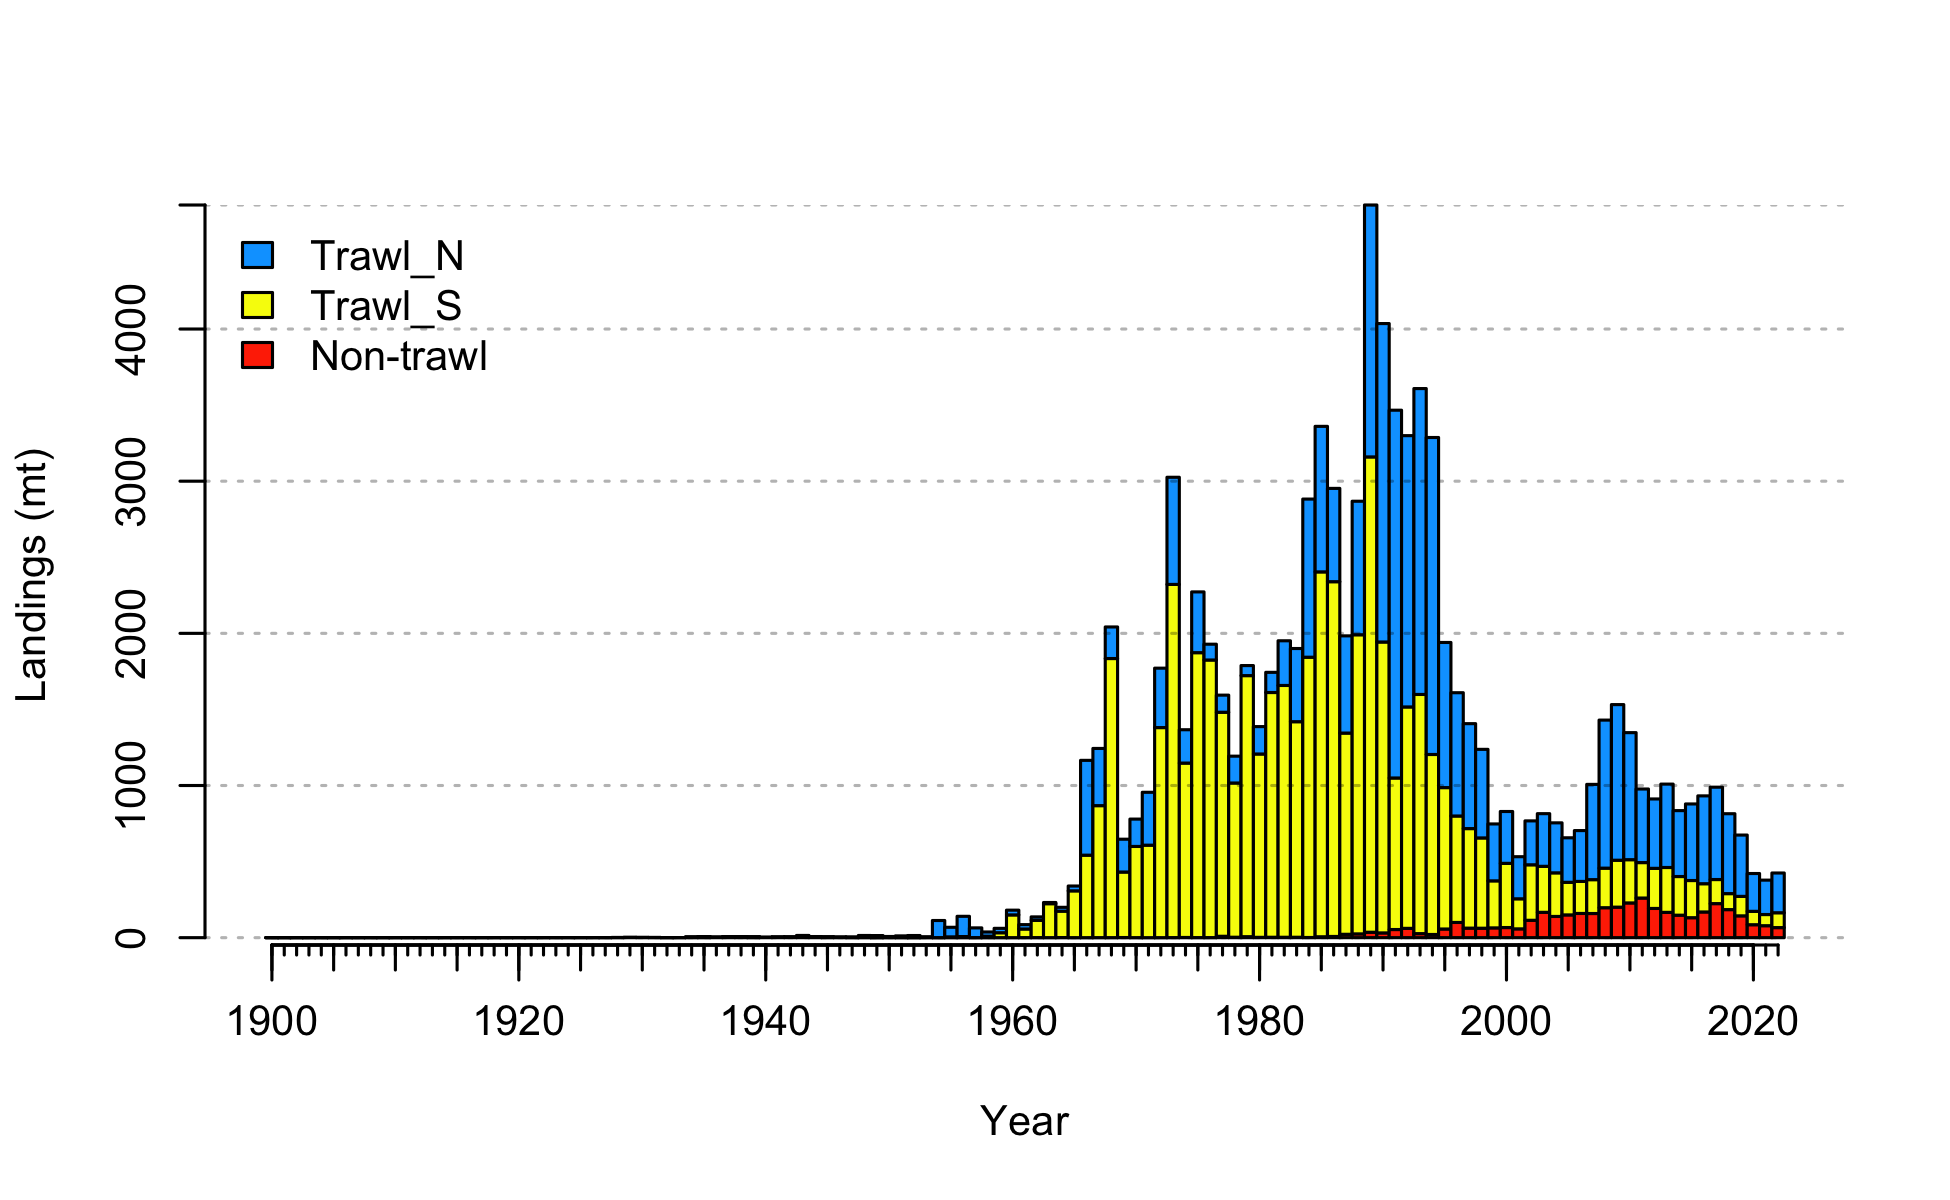
\includegraphics[width=1\textwidth,height=1\textheight]{C:/GitHub/Official_shortspine_thornyhead_2023/doc/FinalFigs/Base/catch2 landings stacked.png}
\caption{Estimated landing history for shortspine thornyhead.\label{fig:catch_histES}}
\end{figure}

\hypertarget{data-and-assessment}{%
\subsection*{Data and assessment}\label{data-and-assessment}}
\addcontentsline{toc}{subsection}{Data and assessment}

The most recent assessment for shortspine thornyhead was conducted in 2013 (Taylor and Stephens 2013). Stock status was determined to be above the management target and catches did not attain the full management limits, so reassessment of thornyheads has not been a higher priority. This assessment uses Stock Synthesis (Methot and Wetzel 2013) Version 3.30.21, used in many other recent US West Coast assessments.

Data were divided into three fishery fleets: North trawl (the waters off Washington and Oregon including the At-Sea Hake fishery), South trawl (the waters off California), and coastwide Non-trawl, and three survey fleets: the \gls{s-tri} from 1980-2004, which was divided into early (pre-1995) and late period (post-1995) to account for a change in depth-sampling, and the \gls{s-wcgbt}, 2003-2022 (Figure \ref{fig:assessment_data_timeseriesES}).

Most data used in the 2013 assessment were newly pulled and processed for this assessment, including length compositions from all fishing and survey fleets, indices of abundance derived from new geostatistical analyses, discard rates from both a 1980s observer study (Pikitch et al. 1988) and the current \gls{wcgop}, historical catch data from Washington, Oregon, and California, and all reported catches from 1981-2022. The only data taken from the previous assessment without reanalysis were discard rates from the \gls{edcp} study in the 1990s.

New maturity analyses of samples collected by the \gls{s-wcgbt} in 2011, 2013, 2014, 2016 and 2018 were available for this assessment (Melissa Head, \gls{nwfsc}, pers. comm.). The larger number and better spatial coverage of these samples allowed the use of statistical modeling to better understand the spatial variation in the proportion of females spawning. This assessment also assumes a new fecundity relationship, in which fecundity is modeled as a power function of length. New growth curves were estimated, using data from Butler (1995), which were similar to the curves assumed in the 2005 and 2013 assessments. In the previous assessment, a Beverton-Holt stock recruitment relationship was assumed and steepness (\(h\)) was fixed at 0.60. This assessment fixed steepness at 0.72, as recommended by Thorson et al. (2019). Natural mortality (\(M\)) was also updated, from 0.0505 in the 2013 assessment, to be fixed at 0.04.

This assessment estimated 197 parameters. The log of the unfished equilibrium recruitment, \(ln(R_0)\), controls the scale of the population and annual deviations around the stock-recruit curve (135 parameters) allow for more uncertainty in the population trajectory. In addition, 59 selectivity and retention parameters for the three fishery fleets and three surveys allowed for estimation of annual length compositions and discards rates. Two catchability parameters were analytically computed from the data, and one additional parameter, representing additional variability in the early Triennial survey, was directly estimated by the model.

\begin{figure}
\centering
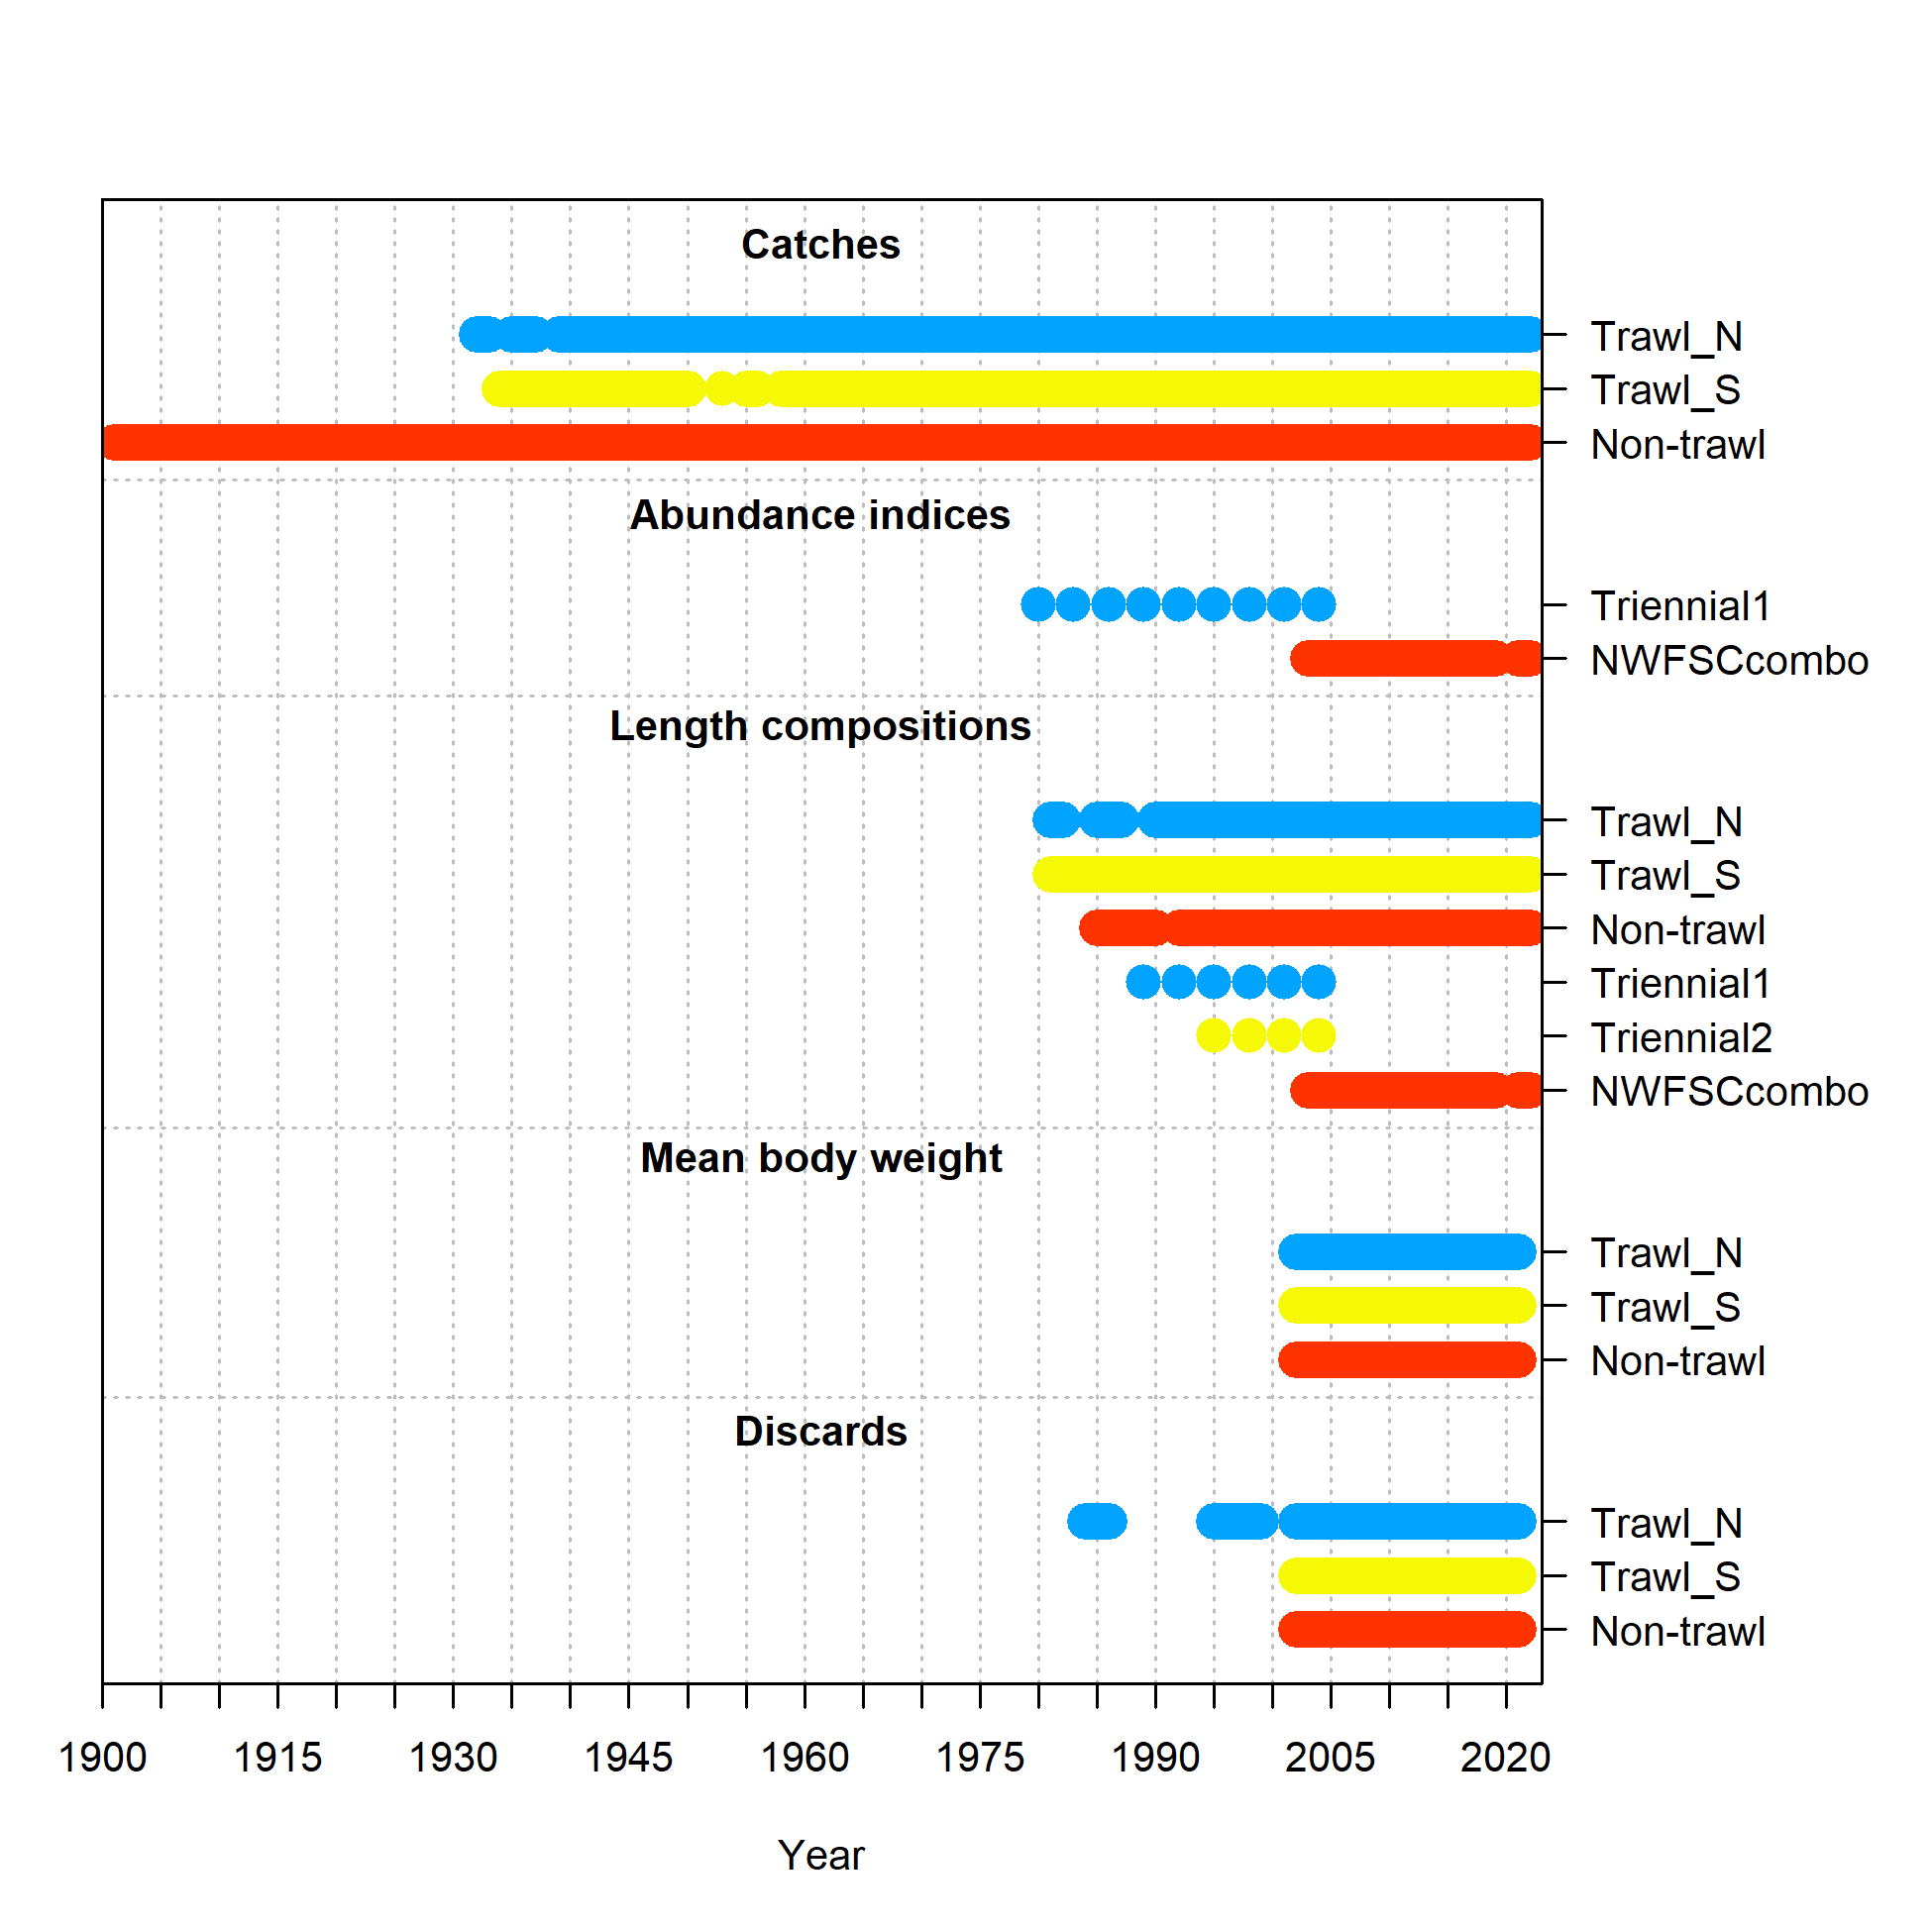
\includegraphics[width=0.8\textwidth,height=1\textheight]{C:/GitHub/Official_shortspine_thornyhead_2023/doc/FinalFigs/Data/data_plot.png}
\caption{Summary of data sources used in the base model.\label{fig:assessment_data_timeseriesES}}
\end{figure}

\hypertarget{stock-biomass-and-dynamics}{%
\subsection*{Stock biomass and dynamics}\label{stock-biomass-and-dynamics}}
\addcontentsline{toc}{subsection}{Stock biomass and dynamics}

Unfished equilibrium spawning output (\(B_0\)) is estimated to be 22.145 trillion eggs, with a 95\% confidence interval of 18.166-26.124 trillion eggs. The \(B_0\) estimate here is not comparable to previous assessment as the integration of new fecundity and maturity assumptions have changed the output units from traditional biomass to spawned eggs. Spawning output is estimated to have remained stable until the early-1970s before beginning to decline near linearly through the present day. The estimated spawning output in 2023 is 8.717 trillion eggs (5.545-11.889 trillion eggs), which represents a stock status or ``depletion'' (\(B_{2023}/B_0\)) of 39.4\% (31.6\%-47.1\%; Table \ref{tab:ssbES}; Figure \ref{fig:ssb_trajectoryES}). The depletion in 2013 was estimated to be 43.5\%, a large decrease from what was estimated by the 2013 assessment (\textasciitilde75\%). The standard deviation of the log of spawning biomass in 2023 is 0.18, which is less than the 0.36 minimum assumed for use in \(p^*\) adjustments to \gls{ofl} values.

\begin{figure}
\centering
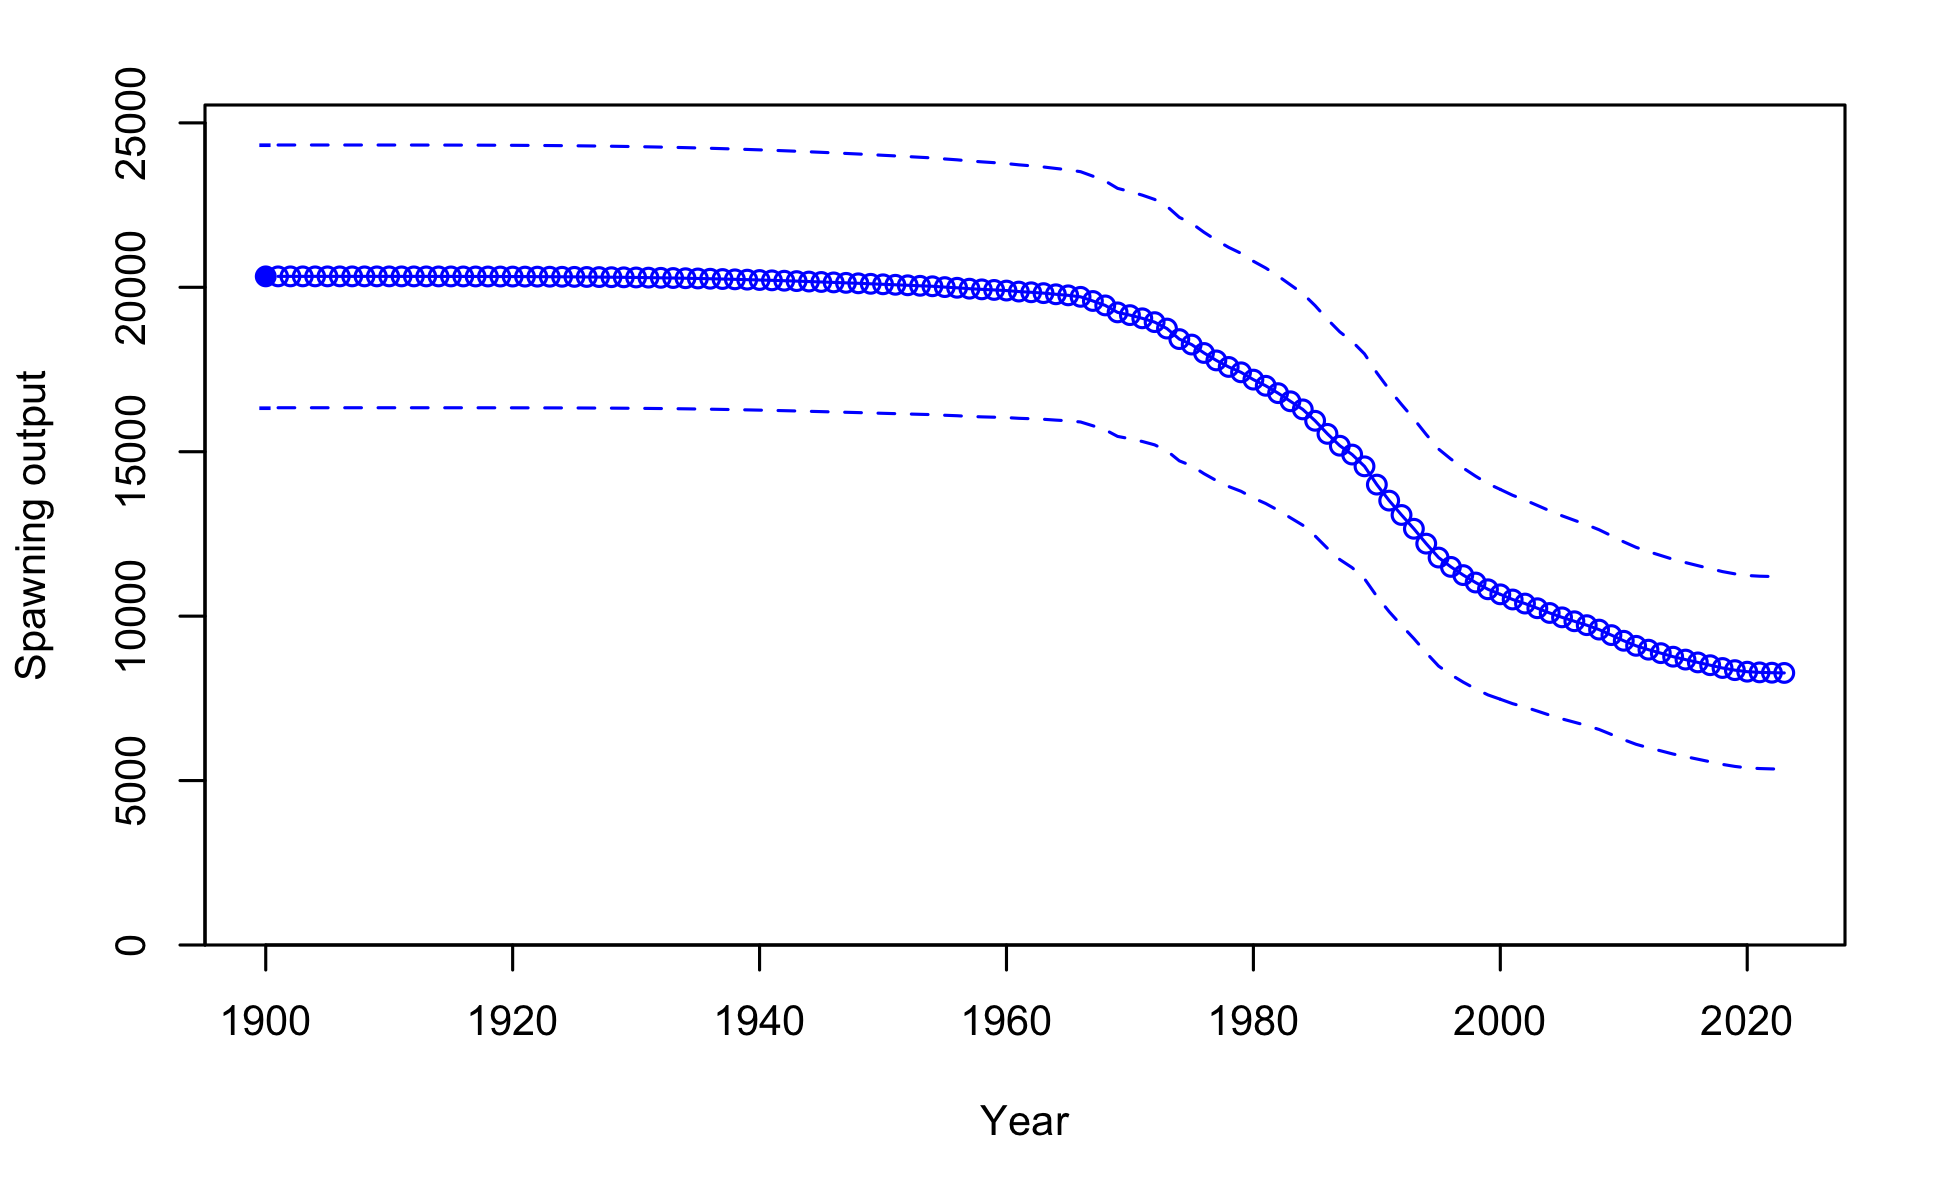
\includegraphics[width=1\textwidth,height=1\textheight]{C:/GitHub/Official_shortspine_thornyhead_2023/doc/FinalFigs/Base/ts7_Spawning_output_with_95_asymptotic_intervals_intervals.png}
\caption{Estimated spawning output trajectory for shortspine thornyhead.\label{fig:ssb_trajectoryES}}
\end{figure}

\begingroup\fontsize{10}{12}\selectfont
\begingroup\fontsize{10}{12}\selectfont

\begin{longtable}[t]{c>{\centering\arraybackslash}p{2cm}>{\centering\arraybackslash}p{2.5cm}>{\centering\arraybackslash}p{2cm}>{\centering\arraybackslash}p{3cm}}
\caption{\label{tab:ssbES}Spawning output (millions of eggs) and fraction unfished with associated 95\% confidence intervals (CI) from the base model.}\\
\toprule
Year & Spawning Output & Spawning Output 95\% CI & Fraction Unfished & Fraction Unfished 95\% CI\\
\midrule
\endfirsthead
\caption[]{\label{tab:ssbES}Spawning output (millions of eggs) and fraction unfished with associated 95\% confidence intervals (CI) from the base model. \textit{(continued)}}\\
\toprule
Year & Spawning Output & Spawning Output 95\% CI & Fraction Unfished & Fraction Unfished 95\% CI\\
\midrule
\endhead

\endfoot
\bottomrule
\endlastfoot
2013 & 9,626 & 6,360–12,892 & 0.435 & 0.360–0.509\\
2014 & 9,476 & 6,228–12,724 & 0.428 & 0.353–0.503\\
2015 & 9,348 & 6,116–12,579 & 0.422 & 0.347–0.497\\
2016 & 9,228 & 6,011–12,444 & 0.417 & 0.341–0.492\\
2017 & 9,112 & 5,908–12,315 & 0.411 & 0.336–0.487\\
2018 & 8,997 & 5,804–12,190 & 0.406 & 0.330–0.482\\
2019 & 8,902 & 5,718–12,086 & 0.402 & 0.325–0.478\\
2020 & 8,829 & 5,651–12,006 & 0.399 & 0.322–0.475\\
2021 & 8,787 & 5,614–11,960 & 0.397 & 0.320–0.474\\
2022 & 8,754 & 5,583–11,925 & 0.395 & 0.318–0.473\\
2023 & 8,717 & 5,545–11,889 & 0.394 & 0.316–0.471\\*
\end{longtable}
\endgroup{}
\endgroup{}

\hypertarget{recruitment}{%
\subsection*{Recruitment}\label{recruitment}}
\addcontentsline{toc}{subsection}{Recruitment}

This assessment assumed a Beverton-Holt stock recruitment relationship. Steepness (\(h\), the fraction of expected equilibrium recruitment associated with 20\% of equilibrium spawning biomass) was fixed at 0.72, slightly higher than what was assumed in previous assessments (\(h=0.60\)). The scale of the population is largely determined by the log of unfished recruitment (\(R_0\)), which was estimated to be 9.439. This results in an unfished recruitment of 12,580,000 recruits (10,320,000-14,841,000). Recruitment variation (\(\sigma_R\)) was fixed at 0.50, as was done in the 2013 assessment. Recruitment deviations were estimated for the years 1901 through 2022, and ranged from -0.5 to 1.5 on the log scale. Estimated recruitments do not show high variability, and the uncertainty in each estimate is greater than the variability between estimates (Table \ref{tab:recES}; Figure \ref{fig:rec_trajectoryES}).

\begingroup\fontsize{10}{12}\selectfont
\begingroup\fontsize{10}{12}\selectfont

\begin{longtable}[t]{c>{\centering\arraybackslash}p{2.2cm}>{\centering\arraybackslash}p{2.2cm}>{\centering\arraybackslash}p{2.2cm}>{\centering\arraybackslash}p{2.2cm}}
\caption{\label{tab:recES}Estimated recent trend in recruitment and recruitment deviations and the 95\% confidence intervals (CI) from the base model.}\\
\toprule
Year & Recruitment & 95\% CI & RecDevs & RecDev 95\% CI\\
\midrule
\endfirsthead
\caption[]{\label{tab:recES}Estimated recent trend in recruitment and recruitment deviations and the 95\% confidence intervals (CI) from the base model. \textit{(continued)}}\\
\toprule
Year & Recruitment & 95\% CI & RecDevs & RecDev 95\% CI\\
\midrule
\endhead

\endfoot
\bottomrule
\endlastfoot
2013 & 9,622 & 4,001–23,138 & -0.112 & -1.004–0.781\\
2014 & 9,650 & 3,996–23,304 & -0.105 & -1.002–0.791\\
2015 & 9,783 & 4,016–23,832 & -0.089 & -0.996–0.818\\
2016 & 10,155 & 4,111–25,087 & -0.049 & -0.973–0.875\\
2017 & 9,995 & 4,024–24,828 & -0.062 & -0.992–0.868\\
2018 & 9,990 & 3,990–25,017 & -0.060 & -1.000–0.879\\
2019 & 10,354 & 4,097–26,165 & -0.032 & -0.989–0.926\\
2020 & 10,839 & 4,230–27,777 & 0.007 & -0.968–0.981\\
2021 & 11,299 & 4,349–29,354 & 0.040 & -0.951–1.031\\
2022 & 10,952 & 4,253–28,200 & 0.000 & -0.980–0.980\\
2023 & 10,942 & 4,249–28,177 & 0.000 & -0.980–0.980\\*
\end{longtable}
\endgroup{}
\endgroup{}

\begin{figure}
\centering
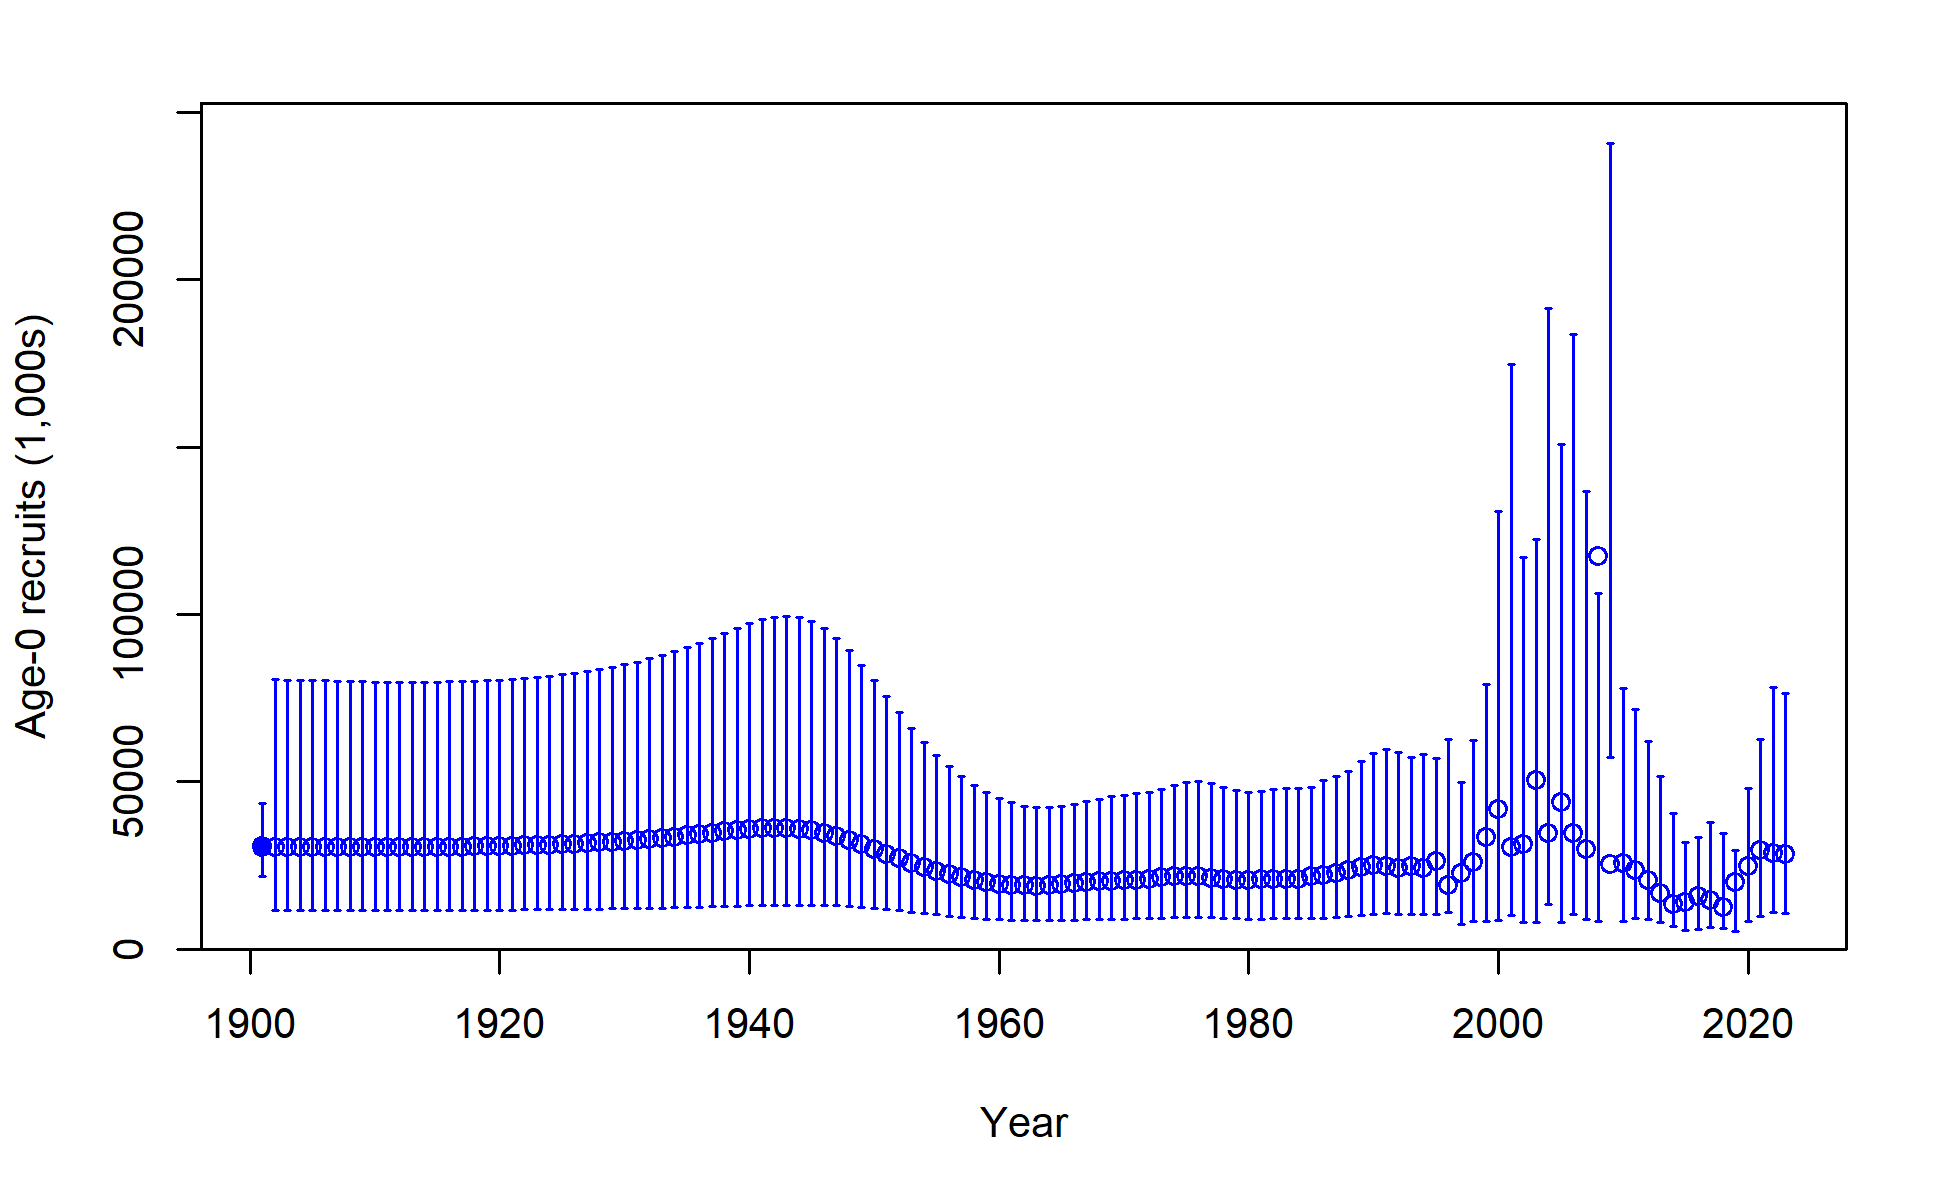
\includegraphics[width=1\textwidth,height=1\textheight]{C:/GitHub/Official_shortspine_thornyhead_2023/doc/FinalFigs/Base/ts11_Age-0_recruits_(1000s)_with_95_asymptotic_intervals.png}
\caption{Estimated recruitment timeseries.\label{fig:rec_trajectoryES}}
\end{figure}

\hypertarget{exploitation-status}{%
\subsection*{Exploitation status}\label{exploitation-status}}
\addcontentsline{toc}{subsection}{Exploitation status}

The summary harvest rate (total catch divided by age-1 and older biomass) closely follows the landings trajectory. The harvest rates are estimated to have never exceeded 5\% and have remained below 2\% in the past decade. Expressing exploitation rates in terms of spawning potential ratio (SPR) indicates that the exploitation consistently exceeded the \(SPR_{50\%}\) reference point from 1980-2018. However, the stock status is estimated to have only fallen below the \(B_{40\%}\) management target starting in 2020 (Table \ref{tab:sprES}; Figures \ref{fig:rel_ssb_trajectoryES}-\ref{fig:phase_diagramES}).

\begingroup\fontsize{10}{12}\selectfont
\begingroup\fontsize{10}{12}\selectfont

\begin{longtable}[t]{c>{\centering\arraybackslash}p{2.2cm}>{\centering\arraybackslash}p{2.2cm}>{\centering\arraybackslash}p{2.2cm}>{\centering\arraybackslash}p{2.2cm}}
\caption{\label{tab:sprES}Estimated recent trend in relative fishing intensity, exploitation rate, and the 95 percent intervals. The spawning potential ratio (SPR) is utilized in the relative fishing intensity calculation as $(1-SPR)/(1-SPR_{40\%})$. }\\
\toprule
Year & (1-SPR)/(1-SPR 50\%) & 95\% CI & Exploitation Rate & 95\% CI\\
\midrule
\endfirsthead
\caption[]{\label{tab:sprES}Estimated recent trend in relative fishing intensity, exploitation rate, and the 95 percent intervals. The spawning potential ratio (SPR) is utilized in the relative fishing intensity calculation as $(1-SPR)/(1-SPR_{40\%})$.  \textit{(continued)}}\\
\toprule
Year & (1-SPR)/(1-SPR 50\%) & 95\% CI & Exploitation Rate & 95\% CI\\
\midrule
\endhead

\endfoot
\bottomrule
\endlastfoot
2013 & 1.29 & 1.06–1.53 & 0.0120 & 0.0079–0.0160\\
2014 & 1.16 & 0.92–1.41 & 0.0100 & 0.0066–0.0134\\
2015 & 1.15 & 0.91–1.40 & 0.0100 & 0.0066–0.0135\\
2016 & 1.19 & 0.95–1.44 & 0.0107 & 0.0070–0.0144\\
2017 & 1.25 & 1.00–1.50 & 0.0118 & 0.0077–0.0159\\
2018 & 1.14 & 0.89–1.39 & 0.0103 & 0.0067–0.0138\\
2019 & 1.00 & 0.75–1.24 & 0.0085 & 0.0055–0.0114\\
2020 & 0.68 & 0.48–0.87 & 0.0051 & 0.0033–0.0069\\
2021 & 0.69 & 0.49–0.88 & 0.0053 & 0.0035–0.0072\\
2022 & 0.88 & 0.66–1.10 & 0.0076 & 0.0050–0.0103\\*
\end{longtable}
\endgroup{}
\endgroup{}

\begin{figure}
\centering
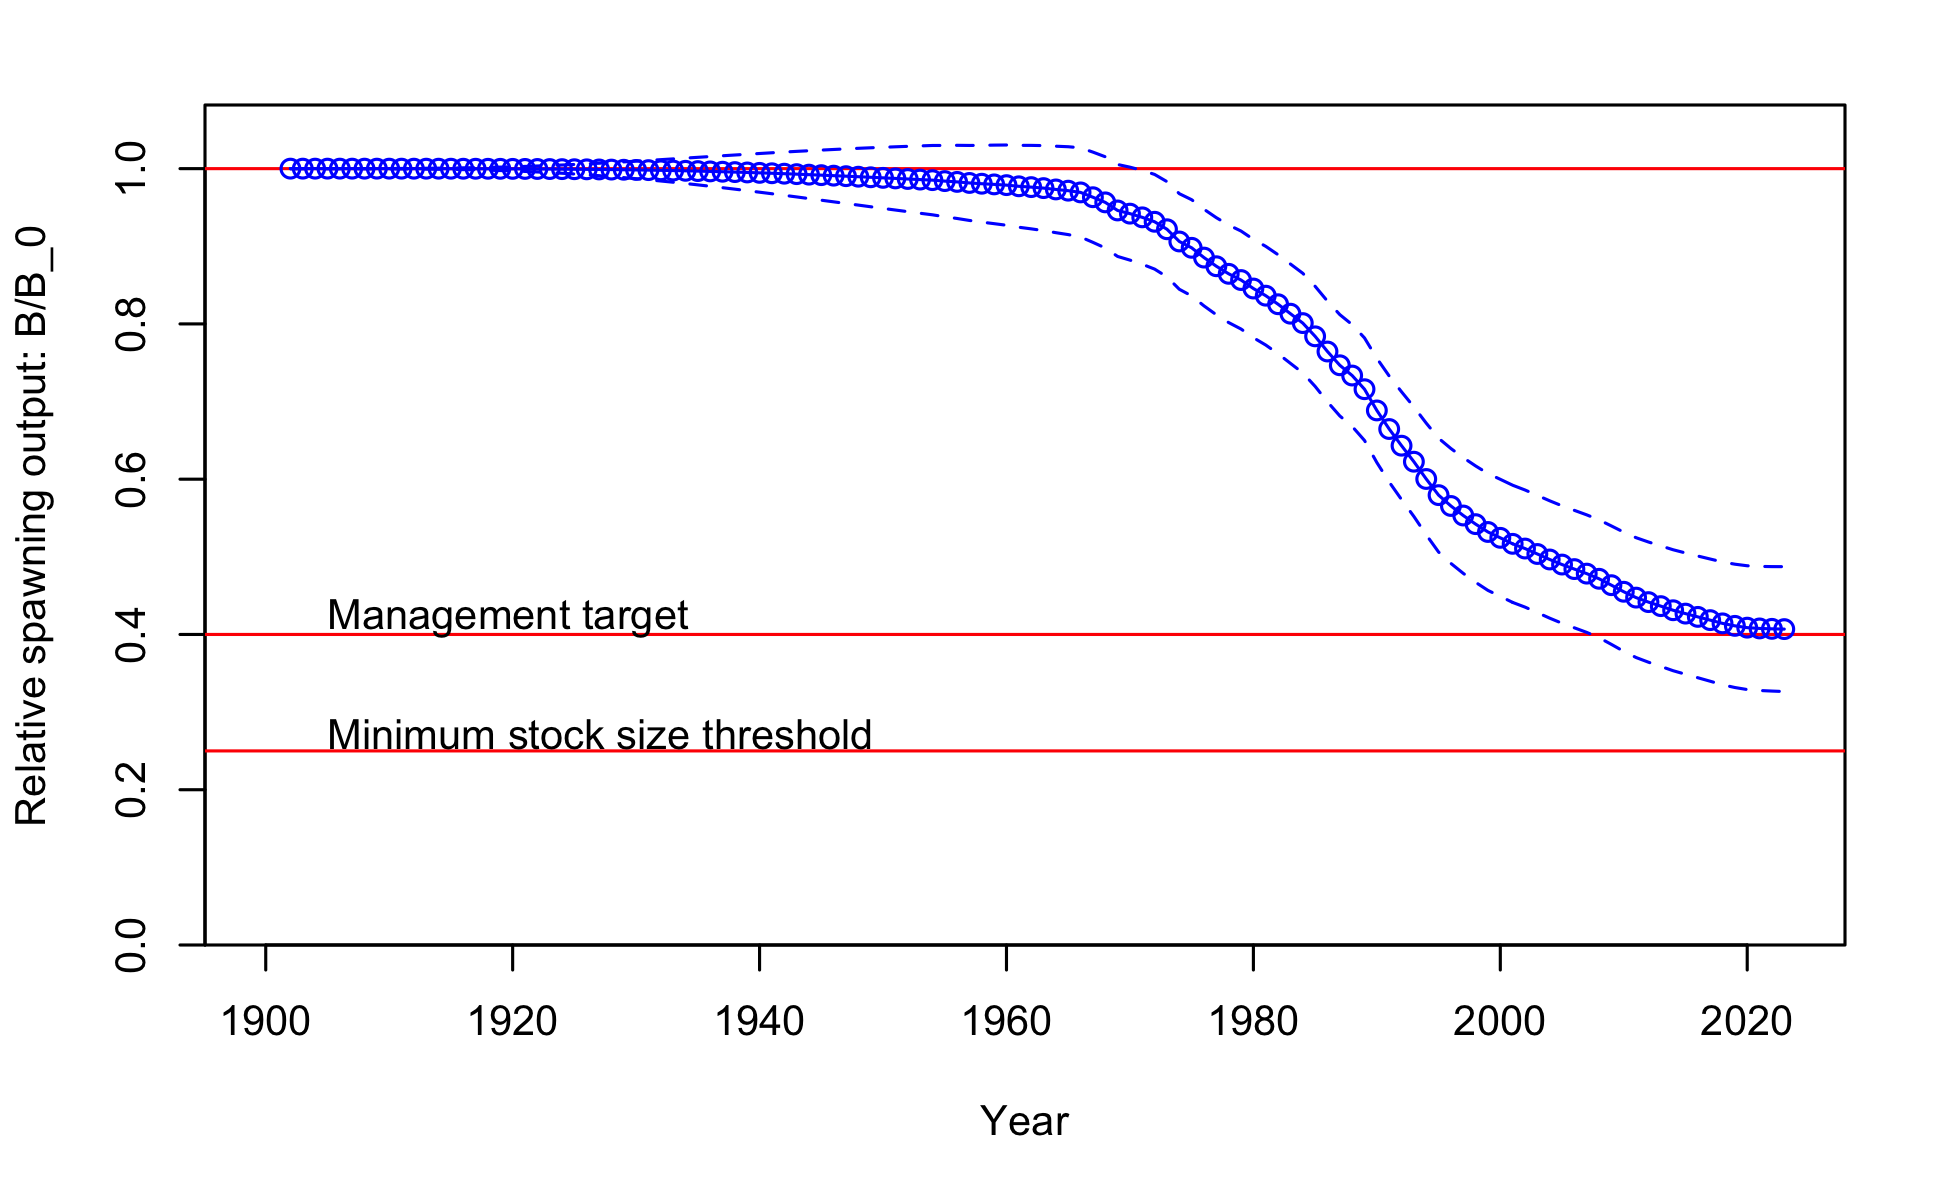
\includegraphics[width=1\textwidth,height=1\textheight]{C:/GitHub/Official_shortspine_thornyhead_2023/doc/FinalFigs/Base/ts9_Relative_spawning_output_intervals.png}
\caption{Estimated spawning output relative to unfished equilibrium for shortspine thornyhead.\label{fig:rel_ssb_trajectoryES}}
\end{figure}

\begin{figure}
\centering
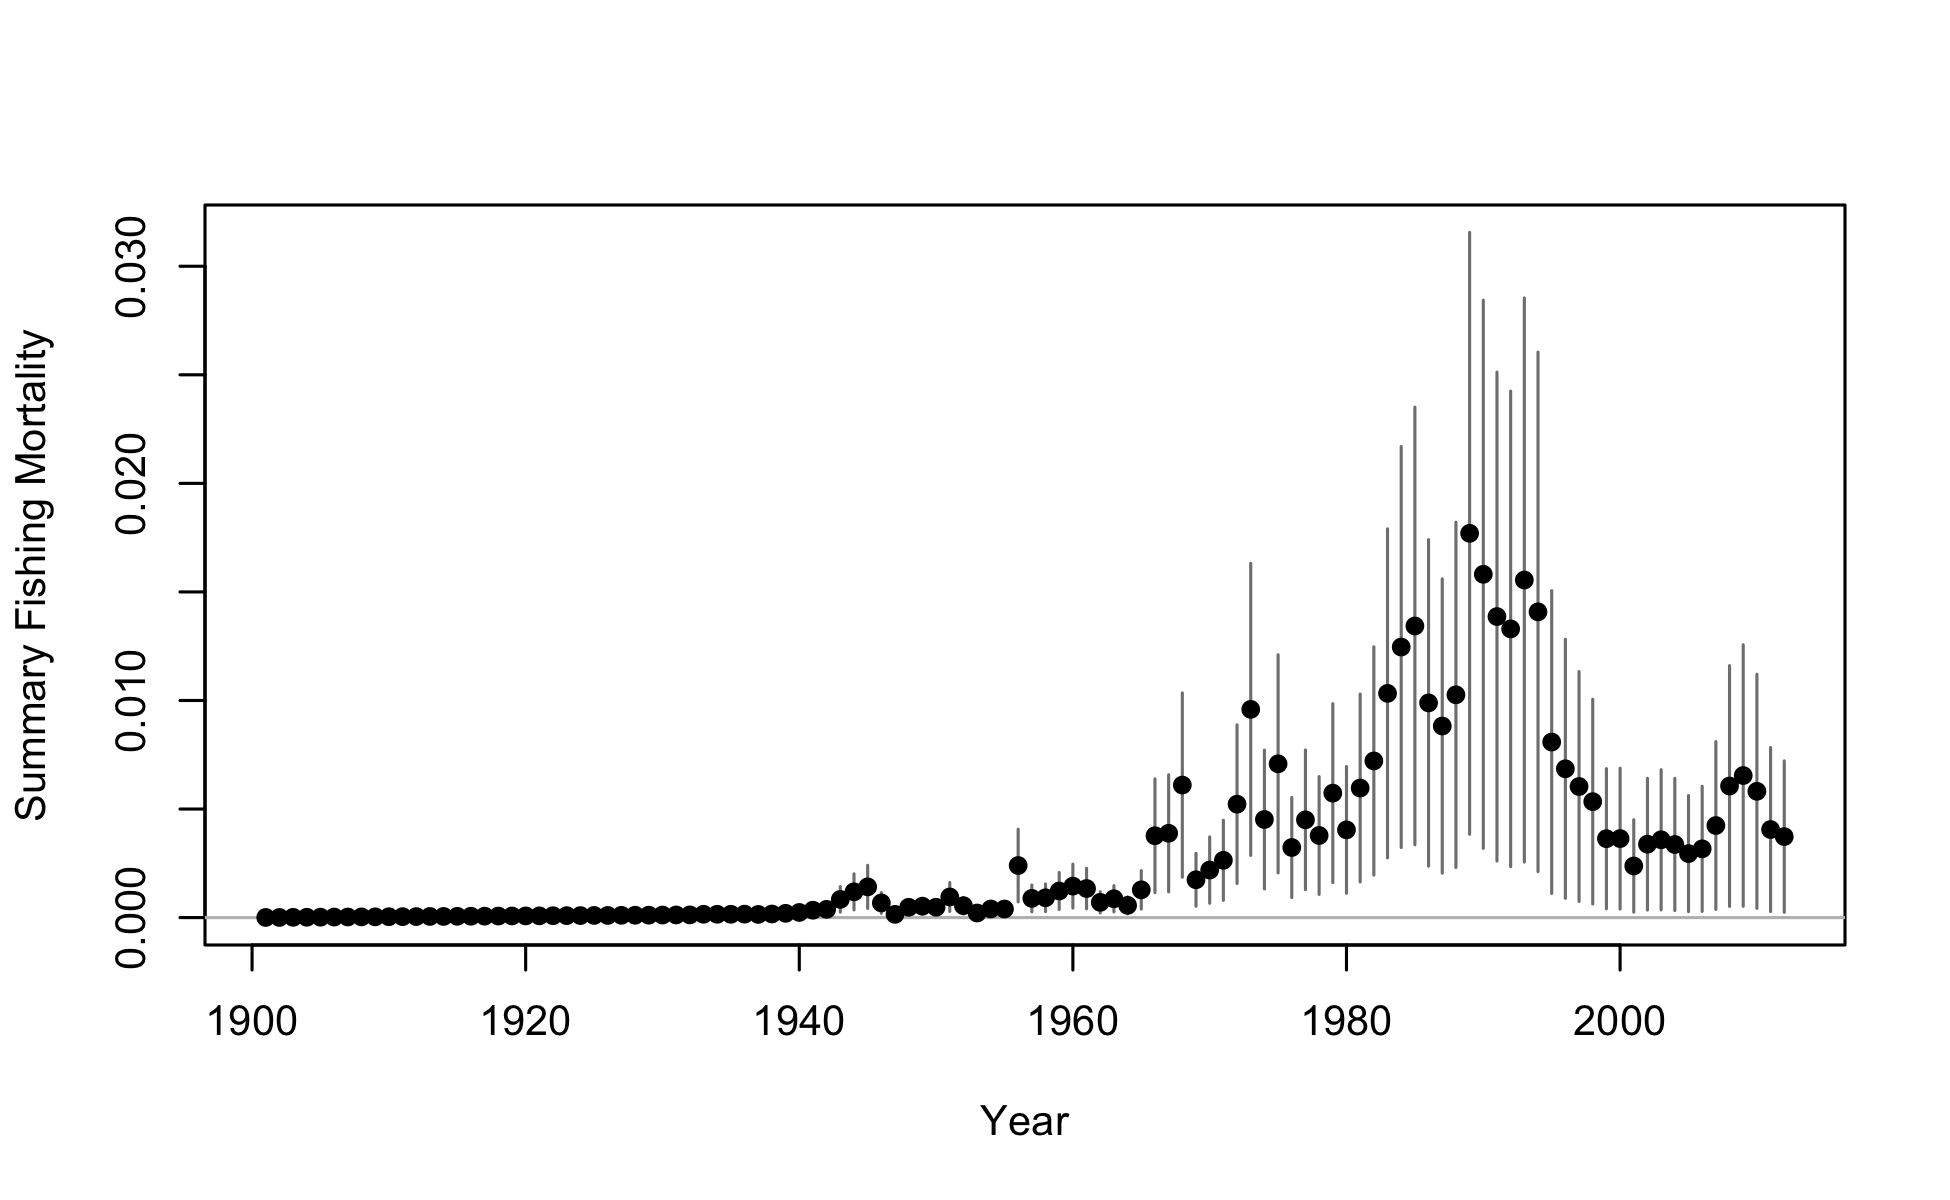
\includegraphics[width=1\textwidth,height=1\textheight]{C:/GitHub/Official_shortspine_thornyhead_2023/doc/FinalFigs/Base/ts_summaryF.png}
\caption{Summary fishing mortality rate (total landings / summary biomass).\label{fig:summary_fES}}
\end{figure}

\begin{figure}
\centering
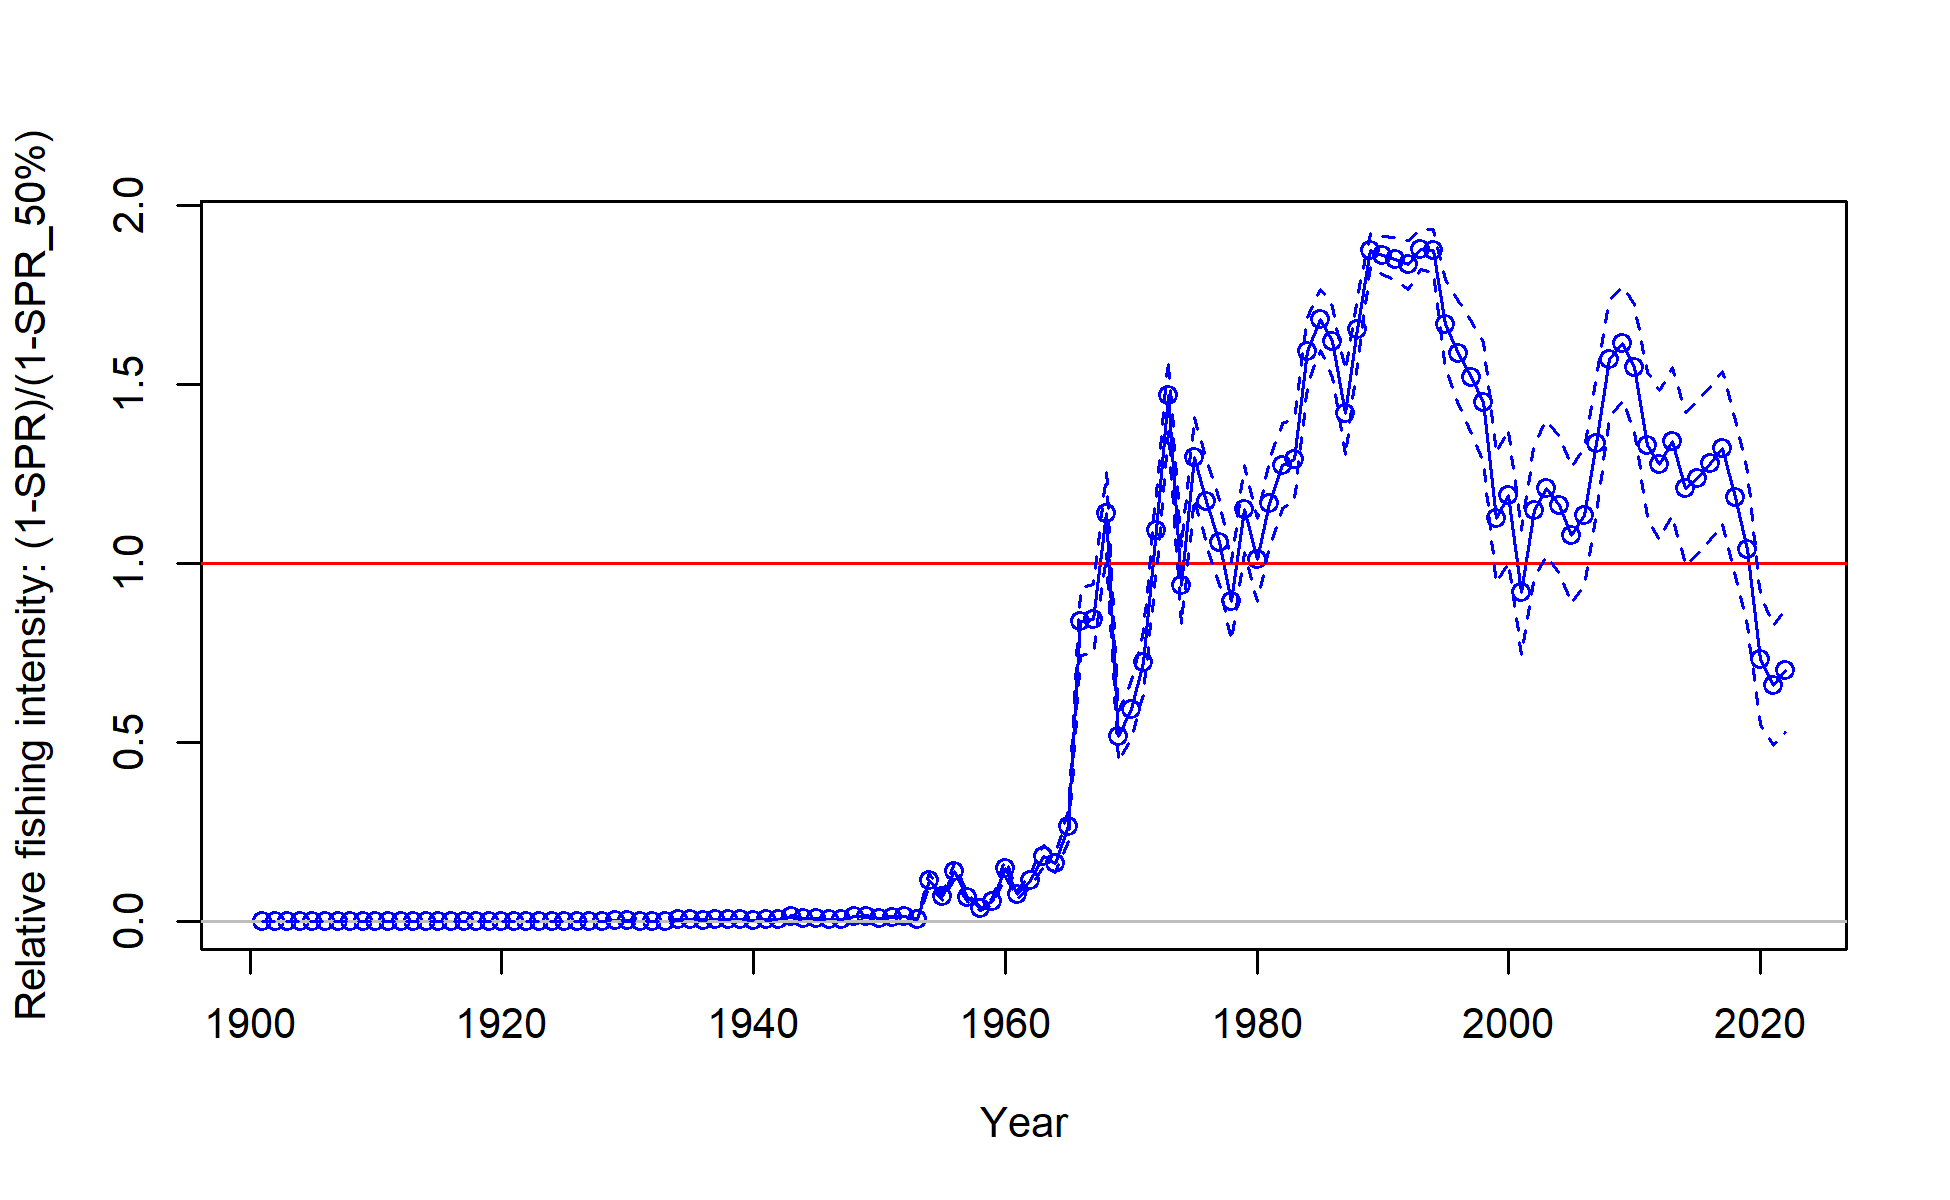
\includegraphics[width=1\textwidth,height=1\textheight]{C:/GitHub/Official_shortspine_thornyhead_2023/doc/FinalFigs/Base/SPR3_ratiointerval.png}
\caption{Estimated relative fishing intensity as a function of spawning potential ratio (SPR).\label{fig:spr_trajectoryES}}
\end{figure}

\begin{figure}
\centering
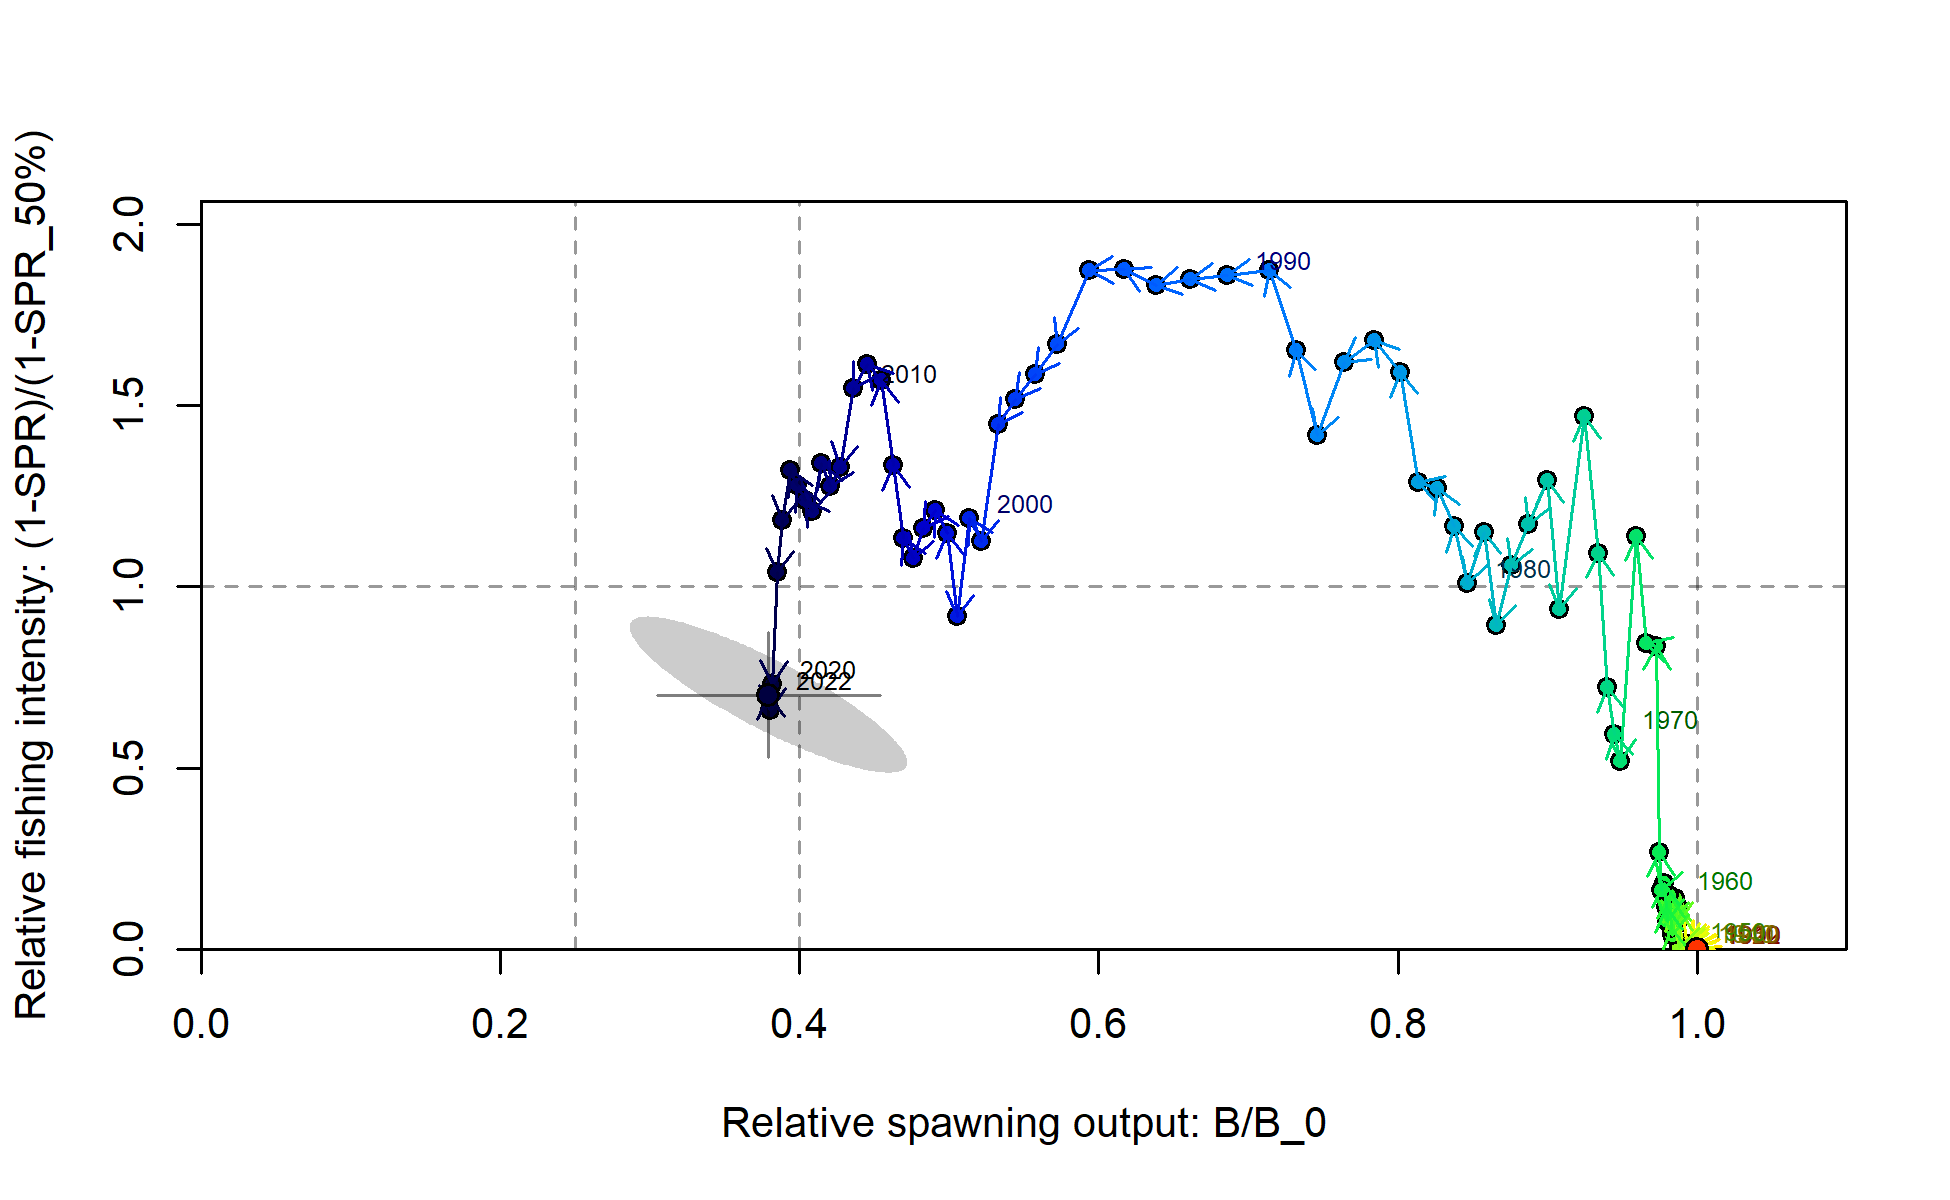
\includegraphics[width=1\textwidth,height=1\textheight]{C:/GitHub/Official_shortspine_thornyhead_2023/doc/FinalFigs/Base/SPR4_phase.png}
\caption{Phase plot of biomass ratio vs.~spawning potential ratio (SPR) ratio. Points represent the annual biomass ratio and SPR ratio. Lines through the final point show 95\% intervals based on the asymptotic uncertainty for each dimension, while the shaded ellipse is a 95\% region accoutninf for estimated correlation between the two quantities.\label{fig:phase_diagramES}}
\end{figure}

\hypertarget{ecosystem-considerations}{%
\subsection*{Ecosystem considerations}\label{ecosystem-considerations}}
\addcontentsline{toc}{subsection}{Ecosystem considerations}

This stock assessment does not explicitly incorporate trophic interactions, habitat factors or environmental factors into the assessment model. More predation, diet, and habitat work, and mechanistic linkages to environmental conditions would be needed to incorporate these elements into the stock assessment.

\hypertarget{reference-points}{%
\subsection*{Reference points}\label{reference-points}}
\addcontentsline{toc}{subsection}{Reference points}

Reference points were calculated using the estimated catch distribution in the final year of the model (2023). In general, the population is on the boundary between ``precautionary'' (\(B/B_0 = 0.40\)) and ``healthy'' (\(B/B_0 > 0.40\)) status relative to the reference points (Figure \ref{fig:yieldcurveES}). Sustainable total yield (landings plus discards) was estimated at 1,108 mt when using an \(SPR_{50\%}\) reference harvest rate and ranged from 929-1,288 mt based on estimates of uncertainty (Table \ref{tab:refPointsES}). The spawning output equivalent to 40\% of the unfished spawning output (\(B_{40\%}\)) was 8.858 trillion eggs. The most recent total mortality (landings plus discards) have been lower than the estimated long-term yields calculated using an \(SPR_{50\%}\) reference point, but not as low as the lower bound of the 95\% uncertainty interval. However, this is due to the fishery not fully attaining the full \gls{acl}. The \gls{ofl} and \gls{abc} values over the past 6 years have been approximately 3100 mt and 2,500 mt, respectively.

\begingroup\fontsize{10}{12}\selectfont
\begingroup\fontsize{10}{12}\selectfont

\begin{longtable}[t]{l>{\raggedright\arraybackslash}p{2cm}>{\raggedright\arraybackslash}p{2cm}}
\caption{\label{tab:refPointsES}Summary of reference points and management quantities, including estimates of the  95\% intervals.}\\
\toprule
Variable of Interest & Estimate & 95\% CI\\
\midrule
\endfirsthead
\caption[]{\label{tab:refPointsES}Summary of reference points and management quantities, including estimates of the  95\% intervals. \textit{(continued)}}\\
\toprule
Variable of Interest & Estimate & 95\% CI\\
\midrule
\endhead

\endfoot
\bottomrule
\endlastfoot
Unfished Spawning Output & 22,145 & 18,166–26,124\\
Unfished Age 1+ Biomass (mt) & 216,864 & 177,897–255,831\\
Unfished Recruitment (R0) & 12,580 & 10,320–14,841\\
Spawning Output (2023) & 8,717 & 5,545–11,889\\
Fraction Unfished (2023) & 0.39 & 0.32–0.47\\
Reference Points Based SB40\% &  & \\
Proxy Spawning Output SB40\% & 8,858 & 7,266–10,450\\
SPR Resulting in SB40\% & 0.458 & 0.458–0.458\\
Exploitation Rate Resulting in SB40\% & 0.012 & 0.011–0.012\\
Yield with SPR Based On SB40\% (mt) & 1,160 & 971–1,348\\
Reference Points Based on SPR Proxy for MSY &  & \\
Proxy Spawning Output (SPR50) & 9,880 & 8,105–11,656\\
SPR50 & 0.500 & -\\
Exploitation Rate Corresponding to SPR50 & 0.010 & 0.010–0.011\\
Yield with SPR50 at SB SPR (mt) & 1,108 & 929–1,288\\
Reference Points Based on Estimated MSY Values &  & \\
Spawning Output at MSY (SB MSY) & 6,155 & 5,057–7,253\\
SPR MSY & 0.348 & 0.345–0.351\\
Exploitation Rate Corresponding to SPR MSY & 0.017 & 0.016–0.017\\
MSY (mt) & 1,227 & 1,027–1,426\\*
\end{longtable}
\endgroup{}
\endgroup{}

\begin{figure}
\centering
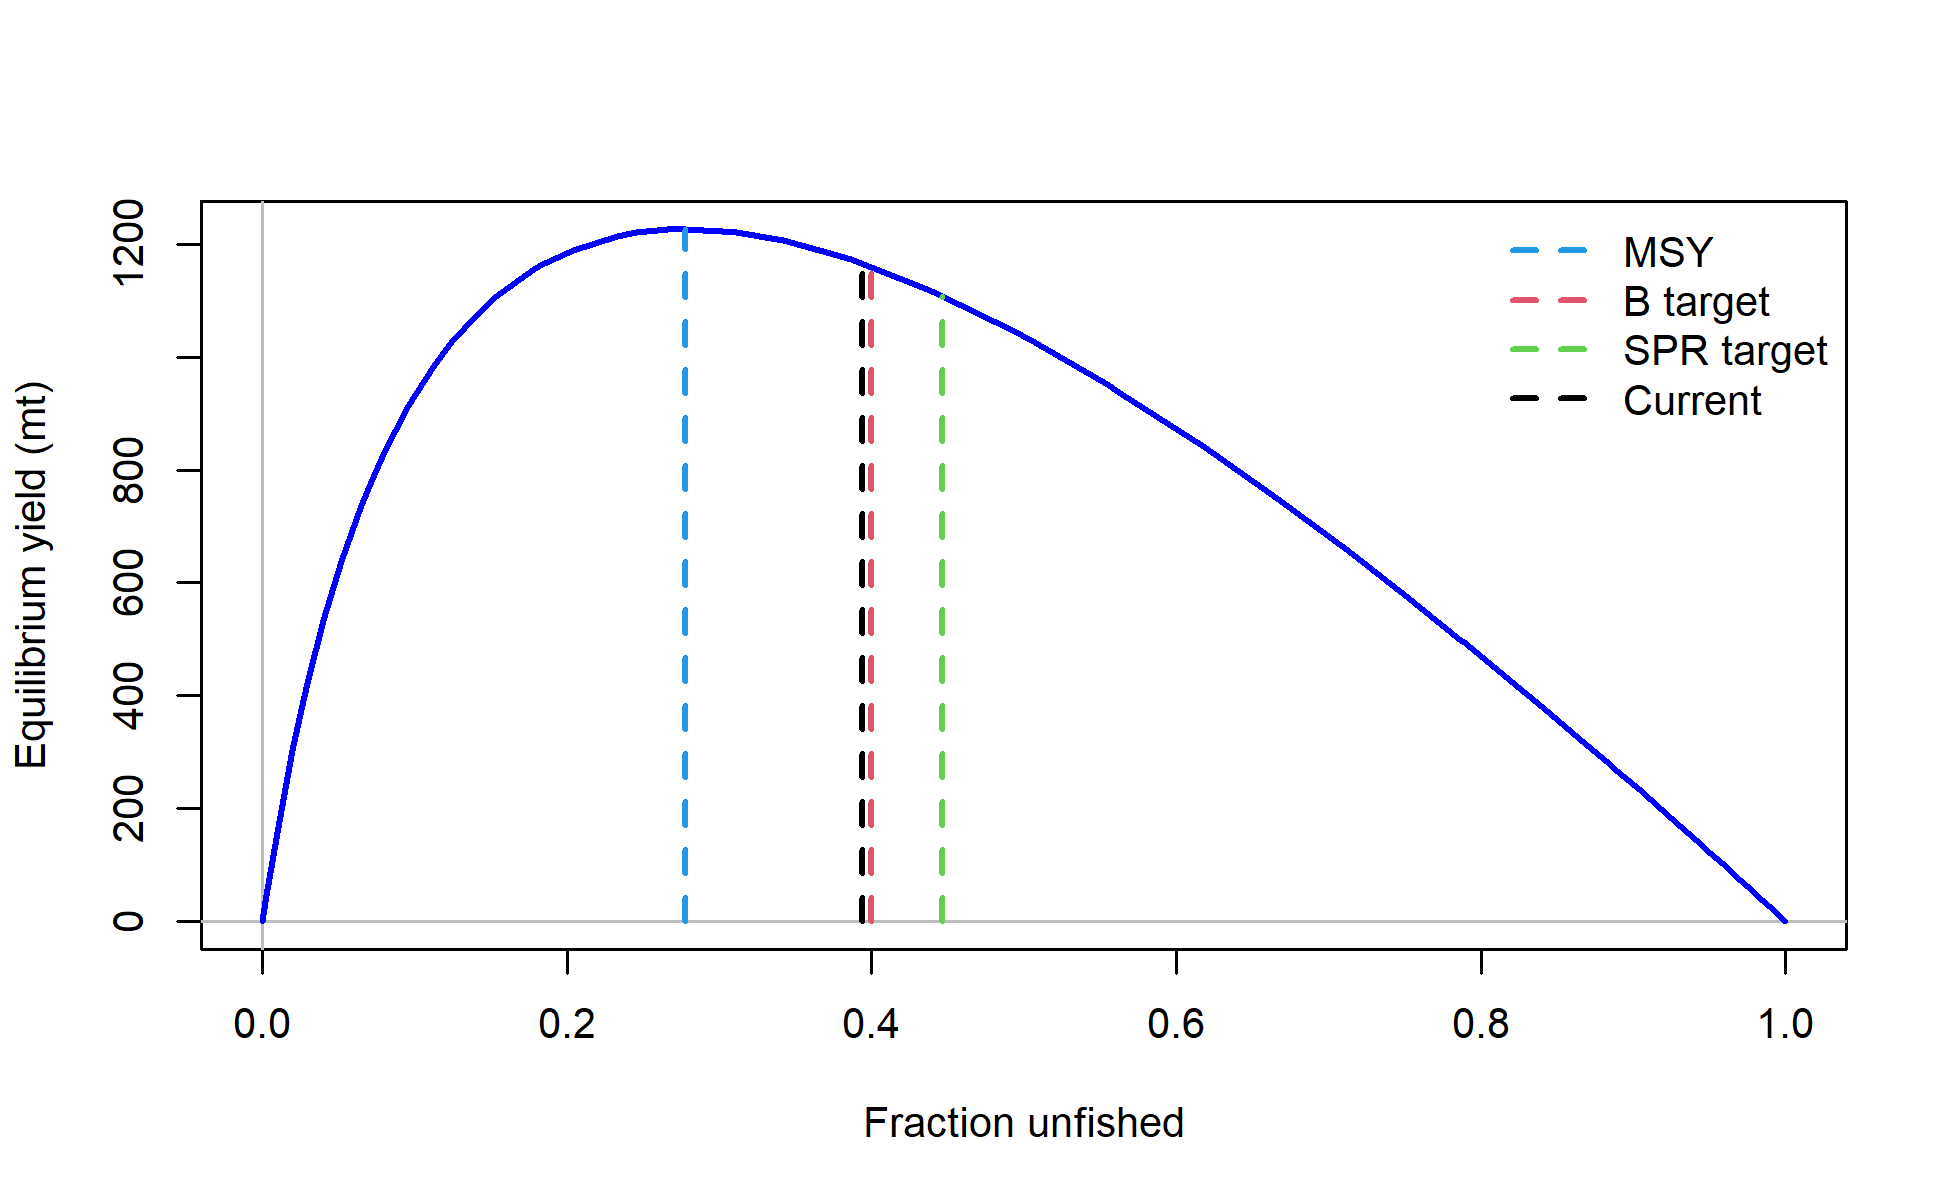
\includegraphics[width=1\textwidth,height=1\textheight]{C:/GitHub/Official_shortspine_thornyhead_2023/doc/FinalFigs/Base/yield2_yield_curve_with_refpoints.png}
\caption{Estimated yield curve with reference points.\label{fig:yieldcurveES}}
\end{figure}

\hypertarget{management-performance}{%
\subsection*{Management performance}\label{management-performance}}
\addcontentsline{toc}{subsection}{Management performance}

Catches for shortspine thornyhead have not fully attained the catch limits in recent years. \Gls{acl}s have hovered around 2500 mt since 2013, while total mortality has never exceeded 1085 mt, and is often smaller than that (Table \ref{tab:managementES}). The fishery for shortspine thornyhead may be limited more by the \gls{acl}s on sablefish, with which they co-occur, and by the challenging economics of deep sea fishing, than by the management measures currently in place. \begingroup\fontsize{10}{12}\selectfont \begingroup\fontsize{10}{12}\selectfont

\begin{longtable}[t]{c>{\centering\arraybackslash}p{1.83cm}>{\centering\arraybackslash}p{1.83cm}>{\centering\arraybackslash}p{1.83cm}>{\centering\arraybackslash}p{1.83cm}>{\centering\arraybackslash}p{1.83cm}}
\caption{\label{tab:managementES}Recent trend in the overfishing limits (OFLs), the acceptable biological catches (ABCs), the annual catch limits (ACLs), the total landings, and total mortality (mt). Total mortality is a function of both landings and model estimated discards.}\\
\toprule
Year & OFL & ABC & ACL & Landings & Total Mortality\\
\midrule
\endfirsthead
\caption[]{\label{tab:managementES}Recent trend in the overfishing limits (OFLs), the acceptable biological catches (ABCs), the annual catch limits (ACLs), the total landings, and total mortality (mt). Total mortality is a function of both landings and model estimated discards. \textit{(continued)}}\\
\toprule
Year & OFL & ABC & ACL & Landings & Total Mortality\\
\midrule
\endhead

\endfoot
\bottomrule
\endlastfoot
2013 & 2333 & 2230 & 1937 & 1,031.34 & 1,111.27\\
2014 & 2310 & 2208 & 1918 & 858.00 & 928.12\\
2015 & 3203 & 2668 & 2668 & 889.26 & 929.06\\
2016 & 3169 & 2640 & 2639 & 942.38 & 992.09\\
2017 & 3144 & 2619 & 2619 & 1,016.94 & 1,094.53\\
2018 & 3116 & 2596 & 2596 & 885.44 & 948.28\\
2019 & 3089 & 2573 & 1983 & 731.55 & 785.62\\
2020 & 3063 & 2551 & 1669 & 431.26 & 477.36\\
2021 & 3211 & 2183 & 2183 & 454.94 & 499.93\\
2022 & 3194 & 2130 & 2130 & 670.12 & 724.14\\*
\end{longtable}
\endgroup{}
\endgroup{}

\hypertarget{unresolved-problems-and-major-uncertainties}{%
\subsection*{Unresolved problems and major uncertainties}\label{unresolved-problems-and-major-uncertainties}}
\addcontentsline{toc}{subsection}{Unresolved problems and major uncertainties}

Major uncertainties in the model are centered around uncertainty in biological processes including growth, maturity, and mortality. The absence of reliable ageing methods for shortspine thornyhead, particularly, makes it difficult to estimate growth and natural mortality.

The assessment does not include age composition data; there is no production ageing of thornyheads for the U.S. West Coast (or Alaska). The assessment model used external estimates of a Von Bertalanffy growth curve based on the Butler research age dataset. The ages in these data were averaged from two age-readers. Nonetheless, there will still be ageing error in the averages. It was also not described how fish were selected for aging or whether they were representative of the overall stock. Age measurement errors and sampling methods are both sources of bias in Von Bertalanffy parameter estimates.

The \gls{s-wcgbt} model-based indices generally followed the design-based trends (Figure \ref{fig:modelbasedsurv}); however, the 2021 and 2022 model-based indices are substantially higher than the design-based indices. Confidence intervals for the model-based indices do not cover the 2021 design-based index, and barely cover the 2022 index. The assessment model could not fit the last two model-based indices which is a potential concern. It is a source of uncertainty why there is such a difference in design- and model-based indices in 2021 and 2022.

Shortspine thornyhead along the Pacific coast could be assessed as a single stock, but recognized that there is a lack of information of recruitment dynamics (e.g., larval transport) that may indicate functional substock structure. These fish do not move much and may be territorial which are attributes that can contribute to substock structure.

There is uncertainty in catch estimates, and more so for historic periods and when interpolations are used to fill in catches for some years. This uncertainty was not quantified and provided to the Panel. There is an important need for STATs to provide information on the quality of the annual catch estimates, and more specifically to quantify the uncertainty in these estimates. This technical deficiency is common to many assessments.

\hypertarget{decision-table-and-projections}{%
\subsection*{Decision table and projections}\label{decision-table-and-projections}}
\addcontentsline{toc}{subsection}{Decision table and projections}

The calculated standard deviation of the log of spawning biomass in 2023 is \(\sigma = 0.18\). This value is ess than the standard , Category 2, sigma on OFL of 1.0, which is therefore used in the adjustment of quotas based on scientific uncertainty. The associated offset would therefore be a multiplication of the OFL by 76.2\% in 2025 and decreasing in future years, which is the 40\% quantile of a log-normal distribution with the associated \(\sigma\). Twelve-year projections were conducted with a total catch assumed equal to the ACL calculated by applying this adjustment to the estimated OFL for each year. The selectivity and retention function and allocation of catch among fleets was assumed to match the values for the 2020-2022 timeblock. Catch for 2023 and 2024, the limits on which have already been set, were provided by the \gls{pfmc}, and correspond to a total catch of 756 mt.

This default harvest projection applied to the base model indicated that the stock status would slowly decline from 39.4\% in 2023 to 39.2\% in 2024, before beginning a slow rebound to 40.1\% by 2034. The associated OFL values over the period 2025--2034 would average 1,022 mt and the average ACL would be 718 mt. These values are near recent annual catch levels.

Additional projections were conducted for the base model and low and high states of nature (columns) under two catch streams (rows) representing different levels of scientific uncertainty, and thus different values of \(P^*\). The uncertainty in the \gls{ofl} associated with the base model was broad (\(\sigma = 0.18\)), and states of nature were chosen based on values of natural mortality (M) that encapsualted the range of M seen in the literature. The low state of nature used \(M=0.03\) to fully encapsulate the low end of the range of M seen in assessments throughout the eastern Pacific. The high state of nature used M=0.05 to roughly encapsulate the value of M used by the 2013 assessment.

The catch streams chosen for the decision table were represented as total catch rather than landed catch, but discard rates were low under IFQs, so the difference in between total catch and landings is small, and represent catch under two distinct levels of P* (\(P^*=0.40\) and \(P^*=0.45\)). The most pessimistic forecast scenario, combining the low state of nature (M=0.03) with the high catch stream (P*=0.45), resulted in a projected stock status of 38.7\%, still very close to the target value, though there is a declining trend owing to a decline in productivity. All other projections led to a higher projected status, with a maximum of 54.7\% for the combination of the high state of nature and low catch. Forecasts under the base case led to estimated depletion values of 39.1\% in both catch scenarios, and incerasing status at near the end of the projection period.

\begingroup\fontsize{10}{12}\selectfont
\begingroup\fontsize{10}{12}\selectfont

\begin{longtable}[t]{c>{\centering\arraybackslash}p{1.38cm}>{\centering\arraybackslash}p{1.38cm}>{\centering\arraybackslash}p{1.38cm}>{\centering\arraybackslash}p{1.38cm}>{\centering\arraybackslash}p{1.38cm}>{\centering\arraybackslash}p{1.38cm}>{\centering\arraybackslash}p{1.38cm}}
\caption{\label{tab:decisiontableES}Summary table of 12-year projections beginning in 2025 for alternate states of nature based on natural mortality. Columns range over low, mid, and high state of nature, and rows range over different assumptions of catch levels.}\\
\toprule
\multicolumn{2}{c}{ } & \multicolumn{2}{c}{Low: M = 0.03} & \multicolumn{2}{c}{Base: 0.04} & \multicolumn{2}{c}{High: M = 0.05} \\
\cmidrule(l{3pt}r{3pt}){3-4} \cmidrule(l{3pt}r{3pt}){5-6} \cmidrule(l{3pt}r{3pt}){7-8}
Year & Catch & SO & Dep & SO & Dep & SO & Dep\\
\midrule
\endfirsthead
\caption[]{\label{tab:decisiontableES}Summary table of 12-year projections beginning in 2025 for alternate states of nature based on natural mortality. Columns range over low, mid, and high state of nature, and rows range over different assumptions of catch levels. \textit{(continued)}}\\
\toprule
Year & Catch & SO & Dep & SO & Dep & SO & Dep\\
\midrule
\endhead

\endfoot
\bottomrule
\endlastfoot
\addlinespace[0.3em]
\multicolumn{8}{l}{\textbf{ACL P* = 0.4}}\\
\hspace{1em}2023 & 756 & 13485 & 0.427 & 8717 & 0.394 & 9907 & \vphantom{1} 0.494\\
\hspace{1em}2024 & 756 & 13334 & 0.422 & 8687 & 0.392 & 9965 & \vphantom{1} 0.497\\
\hspace{1em}2025 & 711 & 13194 & 0.418 & 8666 & 0.391 & 10032 & 0.500\\
\hspace{1em}2026 & 713 & 13067 & 0.414 & 8659 & 0.391 & 10113 & 0.504\\
\hspace{1em}2027 & 716 & 12949 & 0.410 & 8660 & 0.391 & 10202 & 0.509\\
\hspace{1em}2028 & 718 & 12841 & 0.406 & 8670 & 0.392 & 10298 & 0.513\\
\hspace{1em}2029 & 720 & 12742 & 0.403 & 8688 & 0.392 & 10400 & 0.519\\
\hspace{1em}2030 & 721 & 12652 & 0.401 & 8712 & 0.393 & 10509 & 0.524\\
\hspace{1em}2031 & 722 & 12570 & 0.398 & 8744 & 0.395 & 10621 & 0.530\\
\hspace{1em}2032 & 721 & 12496 & 0.396 & 8782 & 0.397 & 10738 & 0.535\\
\hspace{1em}2033 & 720 & 12431 & 0.394 & 8826 & 0.399 & 10857 & 0.541\\
\hspace{1em}2034 & 719 & 12372 & 0.392 & 8874 & 0.401 & 10978 & 0.547\\
\addlinespace[0.3em]
\multicolumn{8}{l}{\textbf{ACL P* = 0.45}}\\
\hspace{1em}2023 & 756 & 13485 & 0.427 & 8717 & 0.394 & 9907 & 0.494\\
\hspace{1em}2024 & 756 & 13334 & 0.422 & 8687 & 0.392 & 9965 & 0.497\\
\hspace{1em}2025 & 815 & 13194 & 0.418 & 8666 & 0.391 & 10032 & 0.500\\
\hspace{1em}2026 & 825 & 13060 & 0.413 & 8652 & 0.391 & 10106 & 0.504\\
\hspace{1em}2027 & 834 & 12934 & 0.409 & 8645 & 0.390 & 10187 & 0.508\\
\hspace{1em}2028 & 843 & 12817 & 0.406 & 8647 & 0.390 & 10275 & 0.512\\
\hspace{1em}2029 & 851 & 12708 & 0.402 & 8655 & 0.391 & 10368 & 0.517\\
\hspace{1em}2030 & 859 & 12607 & 0.399 & 8670 & 0.392 & 10467 & 0.522\\
\hspace{1em}2031 & 866 & 12513 & 0.396 & 8691 & 0.392 & 10569 & 0.527\\
\hspace{1em}2032 & 872 & 12427 & 0.393 & 8717 & 0.394 & 10674 & 0.532\\
\hspace{1em}2033 & 877 & 12348 & 0.391 & 8747 & 0.395 & 10781 & 0.538\\
\hspace{1em}2034 & 883 & 12275 & 0.389 & 8782 & 0.397 & 10889 & 0.543\\*
\end{longtable}
\endgroup{}
\endgroup{}

\hypertarget{scientific-uncertainty}{%
\subsection*{Scientific uncertainty}\label{scientific-uncertainty}}
\addcontentsline{toc}{subsection}{Scientific uncertainty}

The model estimated uncertainty around the 2024 spawning biomass was \(\sigma= 0.18\) and the uncertainty around the \gls{ofl} was \(\sigma = 0.17\). The category 2 default \(\sigma = 1.0\) is used to apply scientific uncertainty in the projections.

\hypertarget{research-and-data-needs}{%
\subsection*{Research and data needs}\label{research-and-data-needs}}
\addcontentsline{toc}{subsection}{Research and data needs}

Research and data needs for future assessments include the following:

\begin{enumerate}
\def\labelenumi{\arabic{enumi}.}
\tightlist
\item
  Research into aging methods and availability of reliable age data would be valuable for future stock assessments. Otoliths have been collected in good quantities from the \gls{s-wcgbt}, but there is currently no validated aging method for shortspine thornyhead.
\item
  Additional investigation into growth patterns would provide valuable information for future population projections. We acknowledge that additional work on aging shortspine thornyhead would be required to make such additional growth research possible. Use of an ``Errors-as-Variables'' approach (e.g.~Dey et al.~2019) could be applied to the Butler growth dataset.
\item
  More investigation into maturity of shortspine thornyhead is necessary to understand the patterns in maturity observed in \gls{s-wcgbt} samples.
\item
  Information on possible migration of shortspine thornyhead would be valuable for understanding stock dynamics. Analysis of trace elements and stable isotopes in shortspine thornyhead otoliths may provide valuable information on the extent of potential migrations. Possible connections between migration and maturity could likewise be explored.
\item
  A greater understanding of the connection between thornyheads and bottom type could be used to refine the indices of abundance. Thornyheads are very well sampled in trawlable habitat, but the extrapolation of density to a survey stratum could be improved by accounting for the proportion of different bottom types within a stratum and the relative density of thornyheads within each bottom type.
\item
  Additional investigation into spatial stock structure could be valuable for determining whether future assessments should develop a spatial assessment model, or if shortspine thornyhead should be assessed at distinct spatial scales in the future.
\item
  Further research into the Dirichilet-Multinmoial (DMN) data-weighting method for length-composition data is needed for integration with length-based data-moderate assessments like shortspine thornyhead. The DMN method has not, to date, been thoroughly simulation tested with length-composition data, and an attempted sensitivity analysis performed for the 2023 assessment failed to converge entirely. This is a general research need, and is widely applicable to many data-moderate or length-based assessments, not just shortspine thornyhead.
\end{enumerate}

\pagebreak
\setlength{\parskip}{5mm plus1mm minus1mm}
\pagenumbering{arabic}
\setcounter{page}{1}
\renewcommand{\thefigure}{\arabic{figure}}
\renewcommand{\thetable}{\arabic{table}}
\setcounter{table}{0}
\setcounter{figure}{0}

\hypertarget{introduction}{%
\section{Introduction}\label{introduction}}

\hypertarget{basic-information}{%
\subsection{Basic Information}\label{basic-information}}

This assessment reports the status of shortspine thornyhead (\emph{Sebastolobus alascanus}) off the US West coast using data through 2022.

Shortspine thornyhead are found in the waters off the West Coast of the United States, from northern Baja California to the Bering Sea, at depths of 20 meters to over 1,500 meters. The majority of the spawning biomass occurs in the oxygen minimum zone between 600 and 1,400 meters. The distribution of the smallest shortspine thornyhead suggests that they tend to settle at 100--400 meters and are believed to exhibit ontogenetic migration down the slope, although large individuals are found across the depth range. Higher densities (kg/ha) of shortspine thornyhead occur in shallower areas (shallow than 400 meters) off Oregon and Washington, whereas in California, they occur in deeper areas (deeper than 400 meters; Figure \ref{fig:stock-map}).

Despite variation in density across the coast, survey data suggest that shortspine thornyheads are present in almost all trawlable areas below 500 meters, as they are caught in 91\% of trawl survey hauls deeper than 500 m. Camera-tows show that thornyheads are spaced randomly across the sea floor, indicating a lack of schooling and territoriality (Wakefield 1990; Du Preez and Tunnicliffe 2011).

\hypertarget{stock-structure}{%
\subsection{Stock Structure}\label{stock-structure}}

Genetic studies of stock structure show few genetic differences among shortspine thornyhead along the Pacific coast, and thus do not suggest separate stocks (Siebenaller 1978; Stepien 1995). Stepien (1995) suggested that there may be a separate population of shortspine thornyhead in the isolated area around Cortes Bank off San Diego, California. Stepien (1995) also pointed out that juvenile dispersion might be limited in the area where the Alaska and California currents split, which occurs towards the northern boundary of the assessment area, near 48° N.

Stepien et al. (2000), using a more discerning genetic material (mtDNA), found evidence of a pattern of genetic divergence in shortspine thornyhead corresponding to geographic distance. However, this study, which included samples collected from southern California to Alaska, did not identify a clear difference between stocks even at the extremes of the range. No such pattern was seen in longspine thornyhead, which suggests that the shorter pelagic stage (\textasciitilde1 yr vs.~\textasciitilde2 yrs) of shortspine thornyhead may contribute to an increased genetic separation with distance.

Dorval et al. (2022) applied otolith microchemistry to immature fish to redefine population structure of shortspine thornyhead on the west coast. Their results indicate that the population of immature shortspines belongs to two distinct groups distributed north and south of Cape Mendocino, California.

\hypertarget{life-history}{%
\subsection{Life History}\label{life-history}}

Shortspine thornyheads along the West Coast spawn pelagic, gelatinous floating egg masses between December and May (Wakefield 1990; Erickson and Pikitch 1993; Pearson and Gunderson 2003). Cooper et al. (2005) and Pearson and Gunderson (2003) found no evidence for batch spawning in this species on the West Coast, but more recent histological examination of ovaries suggest that some shortspine thornyhead can be batch spawners with two to three batches developing simultaneously (Melissa Head, \gls{nwfsc}, pers. comm.). Juveniles settle at around 1 year of age (22- 27 mm in length), likely in the range of 100-200 m (Vetter and Lynn 1997), and migrate down the slope with age and size, although large individuals are found across the depth range.

Shortspine thornyhead are notoriously challenging to age, and a recent age validation study using 14C bomb radiocarbon was inconclusive (Kastelle et al. 2020). However, best available data suggests that the shortspine thornyhead life span may exceed 100 years (Butler 1995; Kline 1996). Estimates of natural mortality for shortspine thornyhead range from 0.013 (Pearson and Gunderson 2003) to 0.07 (Kline 1996). However, the Pearson and Gunderson estimate is based upon a regression model, using the gonadosomatic index as a proxy. Butler (1995) estimated M to be 0.05 based upon a maximum lifespan of 100 years. Butler (1995) also suggested that M may be lower for older, larger shortspine thornyhead residing in the oxygen minimum zone due to lack of predators. All estimates of M for thornyheads are highly uncertain.

Shortspine thornyhead grow very slowly and may continue growing throughout their lives, reaching maximum lengths of over 70 cm. Females grow to larger sizes than males. Maturity in females was previously estimated as occurring near 18 cm, with fish transitioning from immature to mature within a relatively narrow range of sizes between 15 and 20 cm (Pearson and Gunderson 2003). However, more recent histological data of gonads collected in the \gls{s-wcgbt} and analyzed using current best practices suggests that functional maturation, which accounts for abortive maturation and skip spawning, occurs over a broader spectrum of sizes between 10 and 55 cm (length-at-50\% maturity, \(L_{50} =31.4\); personal communication, Melissa Head, \gls{nwfsc}, pers. comm.).

\hypertarget{ecosystem-considerations-1}{%
\subsection{Ecosystem Considerations}\label{ecosystem-considerations-1}}

Shortspine thornyhead have historically been caught alongside longspine thornyhead in a \gls{dts}. Other groundfishes that frequently co-occur in deep waters include a complex of slope rockfishes, Rex sole, longnose skate, roughtail skate, Pacific grenadier, giant grenadier, and Pacific flatnose. Non-groundfish species such as Pacific hagfish and a diverse complex of eelpouts also co-occur with shortspine thornyhead.

Shortspine thornyhead typically occur in shallower water than the shallowest longspine thornyhead, and migrate to deeper water as they age. The majority of spawning shortspine thornyheads occur between 600 and 1,400 meters, where longspine thornyhead are most abundant (Jacobson and Vetter 1996; Bradburn et al. 2011). When shortspine thornyhead have reached a depth where they overlap with longspine thornyheads, they are typically larger than the largest longspine thornyhead.

Species distribution models developed by Liu et al. (in press) suggest that expected environmental changes over the next decades will lead to a decline in shortspine and increase in longspine abundance. Shortspine thornyhead are also projected to shift offshore, into deeper waters, potentially decreasing their availability in fisheries. To date, shortspine thornyhead have been observed by cameras below the 1280 meter limit of the current fishery and survey, but their distribution, abundance, and ecosystem interactions in these deep waters are relatively unknown. Thornyheads spawn gelatinous masses of eggs which float to the surface, which may represent a significant portion of the upward movement of organic carbon from the deep ocean (Wakefield 1990).

Shortspine thornyhead diet composition, as derived from stomach content collection in the 1980s and 1990s, varied by year (Bizzarro et al. 2023). In some years their diet consisted primarily of invertebrate species including pandalid shrimp, pink shrimp, and Tanner crab, while in others their stomach content was dominated by finfish species such as Pacific cod and Pacific Hake. As prey themselves, shortspine thornyheads were only found in the stomachs of other species in two years, 1991 and 1992 as recorded in the \gls{cctd}, where shortspine thornyhead occurred in sablefish, Pacific hake, and other shortspine thornyhead stomachs (Bizzarro et al. 2023).

\hypertarget{historical-and-current-fishery-information}{%
\subsection{Historical and Current Fishery Information}\label{historical-and-current-fishery-information}}

Harvest of shortspine thornyhead has experienced fluctuations over time due to increased depth range of the fisheries, variable markets, and changes in fisheries management. In the early 1900's, landings were minimal because there were few markets for thornyheads and relatively little trawling at depths where the majority of thornyheads occur. Beginning in the 1930s, thornyhead landings increased as they were landed as incidental catch in the California sablefish fishery. The first significant market for thornyheads began in northern California in the early 1960s, when larger (30-35 cm) thornyhead were sold as ``ocean catfish''. By the early 1980s, the minimum marketable size decreased to 25 cm, and in the late 1980s a market for small thornyheads (\textasciitilde20 cm) developed due to the depletion of a related species (\emph{Sebastolobus machrochir}) off the coast of Japan. The fishery moved into deeper waters with the demand for smaller thornyheads and began catching more longspine thornyheads. This is reflected in the changes in proportion of shortspine to total thornyheads through time, which decreased from around 90\% in 1981 to 40\% in 1994 (Figure \ref{fig:thornyhead-ratio}).

Landings of shortspine thornyheads off the coast of California peaked around 3,500 mt in 1989, and have exceeded those from further north in most years (Figure \ref{fig:catch_hist}). In the northern area off of Oregon and Washington, the fishery grew in the early 1980s, with landings peaking in 1991 at around 2200 mt.

Non-trawl landings of shortspine thornyhead were relatively low prior to the mid-1990s, at which point non-trawl landings, dominantly longline-casught from California, began to increase steadily from less than 5 mt in 1994 to 237 mt in 2011. The increase in non-trawl landings was driven by the development of live-fish markets for thornyheads and the fact that ex-vessel prices associated with the non-trawl landings are much higher than those for the trawl fishery. Nominal prices for line-caught shortspine thornyhead have increased steadily through time, from \textdollar 0.49/lb in 1990 to \textdollar 4.71/lb in 2021. This steady increase is also evident when prices are adjusted for inflation, indicating a real price increase in line-caught shortspines that may help to explain the growth, based on landings, in the non-trawl fishery through time. Trawl prices, on the other hand, increased from \textdollar 0.32/lb in 1990 to a high of \textdollar 0.87/lb in 2002 and have since declined with prices in recent years hovering around \textdollar 0.30/lb.

The foreign fishery off of the West Coast is estimated to have caught approximately 7,400 mt of shortspine thornyhead during the 11 year period from 1966-1976 (Rogers 2003), which is similar to the estimated domestic catch (\textasciitilde8,600 mt) during that same period.

Management measures have contributed to a decline in coastwide landings from an estimated peak of 4,815 mt in 1989 to between 1,000 and 2,000 mt per year from 1995 through 1998. Landings fell below 1,000 mt per year from 1999 through 2006, then rose to 1,531 in 2009 and have declined since (Table \ref{tab:allcatch}).

In 2011, the west coast trawl fishery was rationalized, with the introduction of the Individual Fishing Quota (IFQ) Program. In order to provide more flexibility for fishers on the west coast, NOAA Fisheries implemented the West Coast Groundfish Trawl Fishery Catch Share Program, which allows for the division of catch allocated to the trawl fishery into shares controlled by individuals or cooperatives (West Coast Regional Office n.d.). All vessels that participate in the IFQ program are required to have 100\% observer coverage at all times the vessels are at sea (West Coast Regional Office n.d.).

\hypertarget{summary-of-management-history-and-performance}{%
\subsection{Summary of Management History and Performance}\label{summary-of-management-history-and-performance}}

Beginning in 1989, both thornyhead species were managed as part of a \gls{dts} complex. In 1991, the \gls{pfmc} adopted separate \gls{abc} levels for thornyheads and catch limits were imposed on the thornyhead complex, under the Pacific Coast Groundfish Fishery Management Plan (FMP). A \Gls{hg} were instituted in 1992 along with an increase in the minimum mesh size for bottom trawl fisheries. In 1995 separate landing limits were placed on shortspine and longspine thornyhead and trip limits became more restrictive. Trip limits (predominantly 2-month limits on cumulative vessel landings) have often been adjusted during the year since 1995 in order to not exceed the \Gls{hg} or \gls{oy}. At first, the \gls{hg} for shortspine thornyhead was set higher than the \gls{abc} (1,500 vs.~1,000 mt in 1995-1997) in order to allow a greater catch of longspine thornyhead, which was considered relatively undepleted. In 1999 the \gls{oy} was set at less than 1,000 mt and remained close to that level through 2006. As a result of the 2005 shortspine thornyhead assessment, catch limits increased to about 2,000 mt per year and have remained between 2,000 mt and 3,000 mt per year to present.

Since early 2011, trawl harvest of each thornyhead species has been managed under the \gls{pfmc}'s catch share, or \gls{ifq}, program. Whereas the trip limits previously used to limit harvest restricted only the amount of fish each vessel could land, individual vessels fishing under the catch-share program are now held accountable for all of the quota-share species they catch.

Landings of shortspine thornyhead have been below the catch limits since 1999. The estimated total catch, including discards, has likewise remained below the limit during this period (Table \ref{tab:management}).

\hypertarget{fisheries-off-canada-alaska-andor-mexico}{%
\subsection{Fisheries off Canada, Alaska and/or Mexico}\label{fisheries-off-canada-alaska-andor-mexico}}

Shortspine thornyhead are also caught, dominantly in mixed species trawl fisheries, in Canada and Alaska. Catches of shortspine thornyhead off the coast of Canada have exhibited a similar pattern to those on the U.S. West Coast, with catches increasing in the late 1990s and then decreasing to present. A stock assessment for the coastwide population of shortspine thornyhead in British Columbia was last conducted in 2015 and indicated that shortspine thornyhead stock status in Canada is well above reference points and not overfished (Starr and Haigh 2017).

In Alaska, total thornyhead (shortspine and longspine) catches averaged 1,090 tons between 1977 and 1983 in the Gulf of Alaska and then declined markedly in 1984 and 1985, primarily due to restrictions on foreign fisheries imposed by U.S. management policies. Starting in 1985, catches of thornyheads increased, reaching a peak in 1989 with a total removal of 2,616 mt. Catches averaged about 980 mt between 2003 and 2018, when annual catch began to decrease (Echave et al. 2022). The \gls{afsc} conducts assessments of thornyheads as a mixed stock complex, including shortspine and longspine thornyheads. Similar to the British Columbia assessment, results of the 2022 Alaska Thornyhead complex assessment suggest that Thornyheads are not being subjected to overfishing (Echave et al. 2022).

While the range of shortspine thornyhead extends down into Mexico, there is little information about Mexican catch of shortspine thornyhead and no stock assessment conducted in Mexico.

\hypertarget{data}{%
\section{Data}\label{data}}

Data comprise the foundational components of stock assessment models. The decision to include or exclude particular data sources in an assessment model depends on many factors. These factors often include, but are not limited to, the way in which data were collected (e.g., measurement method and consistency); the spatial and temporal coverage of the data; the quantity of data available per desired sampling unit; the representativeness of the data to inform the modeled processes of importance; timing of when the data were provided; limitations imposed by the Terms of Reference; and the presence of an avenue for the inclusion of the data in the assessment model. Attributes associated with a data source can change through time, as can the applicability of the data source when different modeling approaches are explored (e.g., stock structure or time-varying processes). Therefore, the specific data sources included or excluded from this assessment should not necessarily constrain the selection of data sources applicable to future stock assessments for shortspine thornyhead. Even if a data source is not directly used in the stock assessment they can provide valuable insights into biology, fishery behavior, or localized dynamics.

Data from a wide range of programs were available for possible inclusion in the current assessment model. Descriptions of each data source included in the model (Figure \ref{fig:assessment_data_timeseries}) and sources that were explored but not included in the base model are provided below. Data that were excluded from the base model were explicitly explored during the development of this stock assessment or have not changed since their past exploration in a previous shortspine thornyhead stock assessment. In some cases, the inclusion of excluded data sources were explored through sensitivity analyses.

\hypertarget{fishery-dependent-data}{%
\subsection{Fishery-Dependent Data}\label{fishery-dependent-data}}

\hypertarget{catch-history}{%
\subsubsection{Catch History}\label{catch-history}}

Data from the \Gls{pacfin} spanning 1981-present was used to estimate landings in the North (Oregon and Washington) and South (California) by gear type (Trawl and Non-Trawl) (Figure \ref{fig:catch_hist}). One exception was Oregon data from 2017, which came from ODFW directly due to errors in the PacFIN data. All landings reported for the shortspine thornyhead and nominal shortspine thornyhead categories were considered shortspine thornyhead, whereas landings categorized as unidentified thornyheads were split between longspine thornyhead and shortspine thornyhead by the ratio of identified longspine and shortspine landings to total thornyhead landings for each year-state-gear combination (Figure \ref{fig:thornyhead-ratio}).

Catches prior to 1981 are based on historical reconstructions provided by the respective states and a reconstruction of foreign fleet catch. Oregon landings for 1892-1986 are provided by \gls{odfw} and reconstruction methods are outlined in Karnowski et al. (2014). Shortspine thornyhead landings in Oregon are not available in the \gls{pacfin} data for the years 1981-1986, so the state reconstruction is used for this period instead. Washington landings for 1954-1980 are provided by \gls{wdfw}. Landings prior to the beginning of this data are assumed to be zero. California landings are provided by \gls{cdfw} and \gls{swfsc}, and consist of California commercial data for 1969-1980, and a catch reconstruction documented by Ralston et al. (2010) for 1934-1968. As in the two previous assessments, catch data from Rogers (2003) is used to account for catches by foreign fleets during the years 1966-1976. Foreign catch in the Monterey and Eureka \gls{inpfc} areas is attributed to the South Trawl fleet, while foreign catch in Columbia and Vancouver areas is attributed to the North Trawl fleet, as was the case in the 2013 assessment.

For historical catches prior to 1981, all shortspine thornyhead, nominal shortspine, and unidentified thornyhead landings in the state catch reconstructions are considered shortspine thornyhead. Neither California reconstructions prior to 1978, nor the Karnowski et al. (2014) reconstruction for Oregon, distinguish between shortspine and longspine thornyhead species. It is likely that assigning all thornyhead landings to shortspine overestimates total shortspine landings, however, the overwhelming majority of thornyhead landings were shortspine until the late 1980s when vessels began to move into deeper waters and a distinct fishery targeting longspine thornyhead developed (Hamel 2005; Karnowski et al. 2014).

This treatment of historical thornyhead landings differs from the 2005 and 2013 assessments. The 2005 assessment did not have access to the historical reconstructions used here, and instead imputed shortspine thornyhead landings as 30\% of annual sablefish landings for the years 1901-1961. The 2013 assessment used the same imputed values as the 2005 assessment, but also conducted a sensitivity analysis in which all unassigned thornyheads in historical catch were considered shortspine thornyhead. Stock abundance estimates were found to be largely insensitive to which reconstructions were used (Taylor and Stephens 2013). The imputed historical values used for the 2005 and 2013 assessments will continue to be included as a sensitivity analysis here. Landings after 1961 from the state reconstructions remain very similar to the landings used in the 2013 assessment (Figure \ref{fig:catch_hist}).

Unlike previous assessments, this assessment includes catches from the at-sea Pacific whiting fishery (data received from V. Tuttle, 5/15/2023). It includes both shortspine thornyhead catches, as well as unidentified thornyhead catches (the latter only available 1990 to present). Unidentified catches are apportioned based on the year-specific ratio of shortspine thornyhead to longspine thornyhead. There are only three years where Shortspine thornyheads represented less than 99\% of thornyhead catches. The at-sea hake observer program does not collect length composition data on thornyheads, so these catches are added to the northern trawl fleet, considered the most similar gear to the midwater trawls used for Pacific whiting. Landings from this fishery usually a constitute a very small percentage of total shortspine thornyhead catch, however, catches from this fishery in 2022 comprised nearly 30\% of the total landings. It is believed that changes in behavior by the at-sea Pacific whiting fishery resulted in a substantial increase in the number of encounters with shortspine thornyhead, dramatically increasing total catches for this year.

\hypertarget{discards-and-retention}{%
\subsubsection{Discards and retention}\label{discards-and-retention}}

Predicted discards were based on estimated retention and selectivity for each fleet (Figure \ref{fig:disc_hist}). Discards were informed by four data sources covering three different periods. Data sets included, 1) Pikitch et al. (1988) Discard and Mesh Studies, used to estimate both discard rates and length composition of the northern trawl fleet between 1985 and 1987 (John. R. Wallace, \gls{nwfsc} pers. comm.), 2) the \gls{edcp} covering 1995-1999, which only informed discard rates of the northern trawl fleet, 3) the \gls{wcgop}, which provided discard rates, length composition, and individual average weight for years between 2002 and 2021 for all fleets, and 4) the \gls{gemm} data set, covering the same period as the \gls{wcgop} with catch-share participation information and estimates of discard survival rates.

While the estimates from the first two data sets were directly integrated into the model, fleet discard rates after 2011 were available separately for catch-share and non-catch-share programs. Final, fleet-specific, discard rates were thus computed as the average \gls{wcgop} discard rate weighted by the relative proportion of total landings belonging to the catch-share and non-catch-share, respectively (Figure \ref{fig:disc_rates_WCGOP}). Regardless of the type of data, all estimates derived from these data sets had associated uncertainty accounting for the variability observed within the sample of hauls and fishing trips of each fleet. WCGOP-derived discard rates are an exception as, after the catch share program was initiated in 2011, 100\% of hauls from catch share fleets were observed, while non-catch share vessels were only partially covered (West Coast Regional Office n.d.).

The discard data sources were the same as those used in the 2013 assessment. The main improvements are the increased representativeness of all 4 fleets (11 more years) and more accurate estimates of discard rates from \gls{edcp} that were not ready at the time of the previous assessment. Last, some errors in the previous assessment were corrected regarding the weight units considered for the average individual weight (\gls{wcgop} provides weight as pounds and not as kg).

\hypertarget{fishery-length-compositions}{%
\subsubsection{Fishery Length Compositions}\label{fishery-length-compositions}}

Commercial fishery length-composition data were obtained from \gls{pacfin} for 1978-2023. Due to variations in sampling effort and because the number of fish sampled by port samplers is not proportional to the amount of landed catch in each trip, the observed length data were expanded using the following algorithm using the \texttt{PacFIN.Utilities} package in R (Johnson and Stephens 2023):

\begin{enumerate}
\def\labelenumi{\arabic{enumi}.}
\tightlist
\item
  Length data were acquired at the trip level by sex, year and state.
\item
  The raw numbers in each trip were scaled by a per-trip expansion factor calculated by dividing the total weight of trip landings by the total weight of the species sampled.
\item
  A per-year, per-state expansion factor was computed by dividing the total weight of state landings by the total weight of the species sampled for length in the state.
\item
  The per-trip expanded numbers were multiplied by the per-state expansion factor and summed to provide the coast-wide length-frequency distributions by year.
\end{enumerate}

Only randomly collected samples were used. The sample sizes associated with the length compositions from the fishing fleets are shown in Table \ref{tab:lensamp} (landings) and Table \ref{tab:disclensamp} (discards).

Input sample sizes, \({N_{input}}\), for fishery length frequency distributions by year were calculated as a function of the number of trips and number of fish via the Stewart Method (Ian Stewart, pers. comm.):

\begin{equation} {N_{input} = N_{trips} + 0.138N_{fish}}\qquad\text{ when }\frac{N_{fish}}{N_{trips}}<44 \end{equation}

\begin{equation} {N_{input} = 7.06N_{trips}}\qquad\qquad\qquad\text{ when }\frac{N_{fish}}{N_{trips}}\ge 44 \end{equation}

The method is based on analysis of the input and model-derived effective sample sizes from west coast groundfish stock assessments. A piece-wise linear regression was used to estimate the increase in effective sample size per sample based on fish-per-sample and the maximum effective sample size for large numbers of individual fish.

All length data from commercial fisheries were included in the model with sexes combined. This avoids the possibility of bias due to difficulty in sex determination of thornyheads.

\hypertarget{age-compositions}{%
\subsubsection{Age Compositions}\label{age-compositions}}

No age composition data was used for this assessment because thornyheads are very difficult to age (Patrick MacDonald, \gls{nwfsc}, pers. comm.). Even in directed studies such as those done by Kline (1996) and Butler (1995), there are large inter-reader differences, and a second reading by the same ager can produce a markedly different result. Kline (1996) reported only about 60\% of the multiple reads were within 5 years of each other, and inter-reader differences were as large as 24 years for a sample of 50 otoliths. No production ageing of thornyheads is undertaken at this time for the west coast (or Alaska), although shortspine thornyhead otoliths are routinely collected in the NWFSC trawl survey.

\hypertarget{fishery-independent-data}{%
\subsection{Fishery-Independent Data}\label{fishery-independent-data}}

Four trawl surveys have been conducted on the U.S. west coast over the past four decades.

\hypertarget{section}{%
\subsubsection{\texorpdfstring{\acrlong{s-tri}}{}}\label{section}}

The \gls{afsc} conducted a triennial groundfish trawl survey (the \Gls{s-tri}) on the continental shelf from 1977 to 2001, although the 1977 survey had incomplete coverage and is not believed to be comparable to the later years. A final survey was conducted in 2004 by the \gls{nwfsc} using the same survey design. In 1995, the timing of the survey shifted from mid-July and late September to early June through mid-August. In 1980--1992 the survey had a maximum depth of 366 m, while from 1995 onward, the maximum depth was extended to 500 m. The shallow limit of the survey was 55 m in all years, but for purposes of computing indices, only tows deeper than 100 m were used as shortspine thornyhead are rarely seen at shallower depths.

For some species, the shift in timing between the 1992 and 1995 surveys would be expected to influence their catchability, availability, or distribution. However, thornyheads are believed to be sedentary enough that the change in timing would not be as influential. On the other hand, the increase in depth is expected to significantly increase the range of shortspine thornyhead habitat covered by the survey. In the 2013 assessment, the triennial survey was split into two timeseries, separated by the 366 m depth contour, in order to preserve a time series of maximum duration while eliminating the influence of the increased depth range. The first time series, ``AFSC Triennial Shelf Survey 1'', consisted of 9 data points spanning the range 1980--2004 and covering the depths 100--366 m. The second, ``AFSC Triennial Shelf Survey 2'', consisted of 4 data points spanning 1995--2004 and covering depths 366--500 m. This second time series is recognized as providing little information about stock status due to the limited number of points and depth range, but there was no compelling reason to exclude it from the 2013 assessment. In contrast to the 2013 assessment, this assessment treated the \gls{s-tri} as a single time series for the geostatistical model-based indices, and used a different set of latitudinal and depth-based strata for survey length compositions (see Section 2.2.7).

\hypertarget{and-slope-surveys}{%
\subsubsection{\texorpdfstring{\acrshort{afsc} and \acrshort{nwfsc} Slope Surveys}{ and  Slope Surveys}}\label{and-slope-surveys}}

Starting in the late 1990s, two slope surveys were conducted on the west coast. The \gls{s-aslope} was conducted during the years 1997 and 1999--2001 using the research vessel Miller Freeman. The \gls{s-nwslope} was conducted from 1998--2002, and was conducted cooperatively using commercial fishing vessels. The \gls{s-aslope} was a source of valuable information on the depth distribution and overlap of shortspine and longspine thornyheads in the 1980s, but these early years had a very limited latitudinal range and will not be included. This survey also had a different net and larger roller gear than the \gls{s-nwslope}.

Neither of these surveys were included in the base model, as they represent relatively short temporal scales (4 years for the \gls{s-aslope}, and 5 years for the \gls{s-nwslope}) over a period for which survey data already exists (\gls{s-tri} covers this period, though at a sparser temporal resolution).

\hypertarget{section-1}{%
\subsubsection{\texorpdfstring{\acrlong{s-wcgbt}}{}}\label{section-1}}

In 2003, the design of the \gls{s-nwslope} was modified, and the survey was expanded to cover the shelf and slope between 50 m and 1280 m. This combination shelf-slope survey, ``NWFSC Combo Survey'', more recently known as the \gls{s-wcgbt}, has been conducted every year from 2003 to present with consistent design (note that the survey was not conducted in 2020 due to ongoing concerns about COVID-19). Data for the years 2003--2022 were available for this assessment. The \gls{s-wcgbt} represents the largest number of survey observations, the largest depth range, and the most consistent groundfish sampling program in the history of west coast fisheries. Continuing this time series in a consistent manner is vital for improving estimates of current stock status and detecting any future changes in size distribution or abundance of west coast groundfish.

\hypertarget{survey-stratification}{%
\subsubsection{Survey Stratification}\label{survey-stratification}}

Data from these four (nominally five for design-based indices) fishery-independent surveys were considered for use in this assessment (Figure \ref{fig:survey_data_timeseries}) to estimate abundance. Two distinct survey abundance estimation methods were considered: design-based and geostatistical model-based indices. The 2013 assessment utilized delta-GLMMs, following the methods of Thorson and Ward (2013), to compute their indices of abundances, but these methods are no longer considered best practice within the field and were not considered in this assessment.

The five surveys were stratified based on depth and latitude, similar to how they were in 2013 (Table \ref{tab:surveystrat}). The \gls{s-tri} was divided into two distinct survey time series, split on the year 1995. The early-Triennial time series (1981-1992) was further stratified into four strata: north and south of 42˚N, and shallower and deeper than 200m. The late-Triennial time series (1995-2004) was also further stratified into four strata: north and south of 40˚N, and shallower and deeper than 200m. Note that this stratification scheme, as well as the two timeseries, applied to the \gls{s-tri} length composition data and design-based indices of abundance only. The geostatistical model-based inidices that are used in the base model treate the \gls{s-tri} as a single timeseries of abundance. The \gls{s-aslope} was split into two coast-wide strata: shallow and deeper than 550m. The \gls{s-nwslope} was divided into 6 strata, with breaks dividing southern, central, and northern strata at 40.5º N and 43º N, each of which was further divided with a break at 550 m. The \gls{s-wcgbt} was divided into 7 strata, with two southern strata below 34.5º N, one covering 183--550 m and the other covering 550--1280 m. Two central strata, between 34.5º N and 40.5º N, had the same depth ranges. The latitudinal divide around 34.5º N is associated with changes in sampling intensity. North of 40.5º N, three strata were used, covering the ranges 100--183 m, 183--550 m, and the other covering 550--1280 m. The depth breaks at 183 m and 550 m are also associated with changes in the sampling intensity of the survey and are recommended to be used. South of 40.5º N, there are very few shortspine thornyhead shallower than 183 m, so no shallow stratum was used in these latitudes. The 2013 stratification was reused for the design-based indices as there was not sufficient evidence to support modifying the existing strata.

\hypertarget{design-based-indices-of-abundance}{%
\subsubsection{Design-based Indices of Abundance}\label{design-based-indices-of-abundance}}

Design-based indices of abundance were derived for all surveys (Figure \ref{fig:designbasedsurv}). Note that for these indices of abundance, the \gls{s-tri} was split into two independent time series, separated by the year 1995. The construction of design-based indices mirrors a weighted average approach. For each survey year, an average CPUE is calculated across all tows within a stratum and expanded by area to determine the total estimated biomass. These values are then summed across all strata within the survey to create a time series of design-based indices of abundance. Design-based indices were computed using the official \texttt{nwfscSurvey} R package (Wetzel et al. 2023). Note that design-based indices were not used in the base model, and were only derived for the purposes of sensitivity testing.

\hypertarget{geostatistical-model-based-indices-of-abundance}{%
\subsubsection{Geostatistical Model-based Indices of Abundance}\label{geostatistical-model-based-indices-of-abundance}}

Model-based indices of abundance (Figure \ref{fig:modelbasedsurv}) for all surveys were derived using geostatistical models (Thorson et al. 2015) developed using the R package sdmTMB (Anderson et al. 2022). This approach utilizes geostatistical GLMMs with spatially and spatiotemporally correlated random effects, which can account for variables that cause correlations in the data across space and time. For this reason, the \gls{s-tri} can be, and was, treated as a single time series rather than split into two timeseries based on the introduction of additional sampling at greater depths. For the \gls{s-tri}, the geostatistical model included spatial and spatiotemporal random effects and depth and depth squared as a scaled covariate. Geostatistical models for the \gls{s-nwslope}, \gls{s-aslope}, and \gls{s-wcgbt} surveys were not run with depth as a covariate.

Abundance indices were obtained for models using both gamma and log-normal error structures. There is limited agreement on how best to go about model selection for these types of geostatistical models, and both error structures were tested as sensitivity analyses alongside the simple design-based indices described above. The abundance indices derived from the gamma model were most similar to the design-based indices for the Triennial and WCGBT surveys and were thus used for the base model (indices derived from the log-normal model displayed a similar trend to the gamma model-based indices, and the design-based indices, but were consistently larger in scale).

\hypertarget{length-composition-data}{%
\subsubsection{Length Composition Data}\label{length-composition-data}}

Length-composition data were available for each year of each survey including the \gls{s-aslope}, the \gls{s-nwslope}, the \gls{s-wcgbt}, and the \gls{s-tri}. For the Triennial survey, length compositions were divided into an early period (pre-1995), hereafter referred to as the ``early-period Triennial'' and late period (post-1995), hereafter referred to as the ``late-period Triennial'' survey, to account for the change in depth-sampling, and resulting selectivity, that occurred during the 1995 season. The early-period Triennial survey only uses data from 1989 and 1992 due to limited spatial coverage and sample sizes in other years. For all surveys, each haul consists of a set number of random samples regardless of the amount of catch, decoupling the sample and catch size. Therefore, the length compositions were calculated using an expansion factor to account for differences in the amount of catch that samples represent. An expansion factor (calculated as weight of caught fish divided by weight of fish sampled) is calculated for each haul, multiplied by the number of fish in each size bin, and then summed across hauls. This algorithm is repeated for each spatial stratum. Length composition data were compiled into 34, \(2 cm\), length bins, ranging from 6 to 72 cm. Year-specific length frequency distributions generated for each survey are shown in Figure \ref{fig:survey_comps}.

\hypertarget{frequency-of-occurrence-and-survey-information}{%
\subsubsection{Frequency of Occurrence and Survey Information}\label{frequency-of-occurrence-and-survey-information}}

The frequency of occurrence of shortspine and longspine thornyhead in trawl surveys remains extremely high. 91\% of the tows in the \gls{s-wcgbt} below 500 m have at least one shortspine thornyhead in the catch (and 96\% for longspine thornyhead), similar to the 2013 assessment. The number of survey hauls and shortspine thornyhead sampled available for this assessment is described in Table \ref{tab:survinfo}.

\hypertarget{biological-data}{%
\subsection{Biological Data}\label{biological-data}}

\hypertarget{natural-mortality}{%
\subsubsection{Natural Mortality}\label{natural-mortality}}

Butler (1995) estimated the lifespan of shortspine thornyhead to exceed 100 years and suggested that M was likely less than 0.05. M may decrease with age as shortspine migrate ontogenetically down the slope to the oxygen minimum zone, which is largely devoid of predators for fish of their body size. The 2005 assessment fixed the natural mortality parameter at 0.05, while the 2013 assessment used a prior on natural mortality based on a maximum age of 100 years. The prior had a mean of 0.0505 and a standard deviation on a log scale of 0.5361 (Owen Hamel, \gls{nwfsc}, pers. comm.). For the 2023 base model, natural mortality was fixed at 0.04, between the values used by the Alaska and British Columbuia shortspine thornyhead assessments, and the values used in the most recent West Coast assessments. This implies an \(A_{max}\) of \textasciitilde135 years following the mortality prior of Hamel and Cope (2022).

\hypertarget{maturation-and-fecundity}{%
\subsubsection{Maturation and Fecundity}\label{maturation-and-fecundity}}

\hypertarget{maturity}{%
\paragraph{Maturity}\label{maturity}}

Pearson and Gunderson (2003) estimated a length at 50\% maturity of 18.2 cm on the West Coast, with most females maturing between 17 and 19 cm. This was represented in the 2005 and 2013 assessments by the logistic function, \begin{equation} M(L) = (1 + e^{-2.3(L-18.2)})^{-1}\end{equation}

where L is the length in cm.

The 2013 assessment considered new (at the time) maturity information from ovaries collected for maturity analysis on the 2011 and 2012 \gls{s-wcgbt}. Histological analysis of those samples (Melissa Head, \gls{nwfsc}, pers. comm.) indicated puzzling patterns of spawning by female size and by latitude, with a higher fraction of fish spawning in the north than in the south and a higher fraction of spawning fish in the 20-30 cm range than in the 30-40 cm range. However, due to the complexity of these observed patterns and the known ontogenetic migrations of shortspine thornyhead, samples collected in 2011 and 2013 were not considered adequate for estimation of a new representative maturity curve for the entire shortspine thornyhead population in 2013. However, such a maturity curve was considered in a sensitivity analysis. On the basis of the sensitivity analysis, the 2013 assessment suggested that the slow but steady rate of growth for shortspine thornyhead, with growth still occurring at age 100, reduces the importance of assumptions about maturity because older individuals have significantly higher spawning output due to their much larger size, regardless of the fraction spawning.

New maturity analyses of samples collected on the \gls{s-wcgbt} in 2011, 2013, 2014, 2016 and 2018 were available for the 2023 assessment (Melissa Head, \gls{nwfsc}, pers. comm.). The larger number (\(N\)=397) and better spatial coverage of these samples allowed the use of statistical modeling to better understand the spatial variation in the proportion of female spawning.

In the 2013 assessment, the exploration of maturity analyses from the \gls{s-wcgbt} samples highlighted maturity gradients along latitude and depth. To assess a potential relationship between fish location and the shape of the maturity curve, a \gls{glm} was designed for estimating maturity curve parameters while integrating latitude and depth as covariates. This \gls{glm} consists of a logistic regression in which the functional maturity of samples, modeled with a Bernoulli distribution, is expressed as a linear combination of fish length, latitude, latitude squared, depth and depth squared. Once fitted, the \gls{glm} was used to predict the response of the probability of being mature along the range of individual shortspine thornyhead length considered in the model. For the 2023 assessment, this model prediction was made while setting the latitude and depth at the values of the center of gravity (using number of fish as a weighing factor) of the population of shortspine thornyhead sampled by the \gls{s-wcgbt} to develop a single curve for the coastwide population assessment. Thus, this response of functional maturity to length was considered the mean maturity curve of the west coast shortspine thornyhead population. The parameters of the maturity curve \(L_{50}\) and \(k\) were arithmetically derived from this response to fish length. The new maturity curve is expressed as follows:

\begin{equation} M(L) = (1+e^{-2.3(L-31.42)})^{-1}\end{equation}

Figure \ref{fig:mat1} shows the fit of the maturity curve of the model per class of depth and latitude.

A sensitivity analysis assessed the impact of this change in the maturity curve on the model estimates by considering the newly estimated parameters, the Pearson and Gunderson relationship from 2013, and an intermediate option (Figure \ref{fig:mat2}).

\hypertarget{fecundity}{%
\paragraph{Fecundity}\label{fecundity}}

The previous assessments assumed spawning biomass was equivalent to spawning output. The current assessment uses fecundity-at-length parameters reported in Cooper et al. (2005). Fecundity is modeled as a power function of length:

\begin{equation} F = 0.0544L^{3.978} \end{equation}

where \(F\) is fecundity in the number of eggs per female and \(L\) is length in cm. Cooper et al. (2005) estimated the fecundity of 54 females collected from the West Coast and Alaska. They found no difference in the length-fecundity relationship by region and pooled the samples. That study suggested that fecundity increases at a faster rate with length than body weight with length for shortspine thornyhead, meaning that larger females have greater relative fecundity compared to small females. This assessment models a fecundity-at-length relationship using the fecundity parameters from Cooper et al. (2005) (Figure \ref{fig:fec}) and scaling the fecundity intercept by one million to report fecundity in billions of eggs.

Uncertainty remains in the spawning strategy of shortspine thornyhead. Cooper et al. (2005) and Pearson and Gunderson (2003) found no evidence of batch spawning in this species (i.e., a determinate, total spawning strategy). However, updated histological information suggests a possibility of batch spawning (Melissa Head, NWFSC, pers. comm.). Batch spawning could influence the fecundity-at-length relationship if not properly accounted for and should be a focus of future research.

\hypertarget{length-weight-relationship}{%
\subsubsection{Length-Weight Relationship}\label{length-weight-relationship}}

Fisheries-independent length and weight specimen data were available from the \gls{s-aslope} (1997, 1999-2001; \(N\)=7,623) and the \gls{s-wcgbt} (2003-2021, excluding 2020; \(N\)=20,142). The \gls{s-wcgbt} data were used to estimate the length-weight relationship because it had the largest sample size and covered the greatest spatio-temporal resolution. Unsexed fish \textless16 cm in length, and obvious outliers were removed from the dataset prior to fitting the relationship. The allometric function models weight (\(W\)) as a power function of length (\(L\)), where:

\begin{equation} W = \alpha L^{\beta} \end{equation}

This function can be linearized by taking the natural logarithm of both sides. The predicted weight-at-length values were bias-corrected using a multiplier of \(\sigma^2 / 2\). The length-weight parameters were estimated for both sexes in R using the \texttt{lm()} function (R Core Team 2021).

The resulting parameters for 2023 (females: \(\alpha = 4.86*10^{-6}\), \(\beta = 3.26\); males: \(\alpha = 4.69*10^{-6}\), \(\beta = 3.25\); Figure \ref{fig:lengthweight}) were very similar to the 2013 assessment values, which estimated a single length-weight relationship for males and females combined using \gls{s-wcgbt} data through 2012 (sexes combined: \(\alpha = 4.77*10^{-6}\), \(\beta=3.26\)). The available data suggested that length-weight is highly conserved in shortspine thornyhead; therefore, no sensitivity analysis was conducted for this set of parameters in the 2023 assessment.

\hypertarget{growth-length-at-age}{%
\subsubsection{Growth (Length-at-Age)}\label{growth-length-at-age}}

No validated ageing methods currently exist for shortspine thornyhead; therefore, this species is not aged by the \gls{nwfsc} or \gls{swfsc} and length-at-age data were limited for this stock assessment. Two research age datasets exist for shortspine thornyhead in the West Coast region: (1) Kline (1996) includes 319 unsexed fish collected from Monterey Bay in central California in 1991, and (2) Butler (1995) includes 1,023 sexed fish collected in the waters off northern California and Oregon in 1978-1988 and 1990. The Kline specimens were aged by one age reader, and lengths were reported as total lengths, whereas the Butler specimens were aged independently by two separate age readers, and lengths were reported in fork length. The Butler data age data used in this assessment are the mean ages between the two age readers.

The length-at-age curve developed in the 2005 stock assessment and used again in 2013 was based on a Schnute parameterization of the Von-Bertalanffy growth function fit to the Kline data. The resulting parameter estimates for this growth function were as follows: growth rate \(k\) was 0.018 for both males and females, length at age-2 was 7 cm for both males and females, and length at age-100 was 67.5 cm for males and 75 cm for females based on the assumption that the asymptotic length for males should be 90\% of the asymptotic length for females (Hamel 2005). The data and associated analysis from 2005 were lost; however, the original Kline and Butler datasets were obtained for use in this assessment (Donna Kline, pers. comm., March 2023). Using these newly obtained data, we could not reproduce the parameters used in the 2005 assessment.

Because the Butler data were sex-specific, had a higher sample size, were aged by two readers instead of one, and were collected from a larger geographic area and over more years compared to the Kline data, we determined that Butler was the preferred dataset to estimate the length-at-age relationship for the 2023 stock assessment. We fit sex-specific Schnute growth functions to the Butler data:

\begin{equation} \hat{L}_{a} = L_{a_{1}}+\frac{(L_{a_{2}}-L_{a_{1}})(1-exp(-k(a_{2}-a_{1})))}{(1-exp(-k(a_{2}-a_{1})))}\end{equation}

where: \(L_{a_{1}}\) and \(L_{a_{2}}\) are the lengths at reference ages \(a_{1}\) and \(a_{2}\) where \(a_{1}=1\); \(a_{2}=100\) and \(k\) is the growth rate. Growth curve estimation was conducted in R using the optim() function (R Core Team 2021). Errors were assumed to be lognormally distributed and predicted length-at-age was bias-corrected using a multiplier of \(\sigma^2/2\). Updated growth parameters were fixed in the assessment at the following values using the reference ages and equation described above:

Females: \(L{a_{1}}\) = 11.4 cm; \(L{a_{2}}\) = 73.6 cm; \(k\) = 0.0099 per year\\
Males: \(L{a_{1}}\) = 9.2 cm; \(L{a_{2}}\) = 66.1 cm; \(k\) = 0.0168 per year

For reference, the equivalent von-Bertalanffy growth parameters are:

Females: \(t{_0}\) = -8.931; \(L{_{inf}}\) = 111.0 cm; \(k\) = 0.0099 per year Males: \(t{_0}\) = -5.314; \(L{_{inf}}\) = 79.4 cm; \(k\) = 0.0168 per year

Shortspine thornyhead are slow-growing fish that appear to continue to grow throughout their lifespan (i.e., the growth curve does not asymptote). The new growth curves estimated using the Bulter dataset exhibited similar trends to those assumed in the 2005 and 2013 assessments (Figure \ref{fig:growthcurve}). The male curves were almost identical, with the 2005/2013 curve exhibiting slightly lower length-at-age at young ages and slightly higher length-at-age at older ages. The 2005/2013 female curve was defined by a higher growth rate, leading to the higher length-at-age in the intermediate age range.

Two alternative sensitivity analyses were developed for the 2023 assessment. During the exploratory data analysis phase, we found that specimens collected in the Kline study exhibited higher size-at-age when compared to the Butler specimens (Figure \ref{fig:growthcurve}). It is unknown if these differences should be attributed to spatial differences in growth between central California and northern California/Oregon, bias among age readers, or discrepancies between the total and fork length measurements (Donna Kline, pers. comm., March 2023). In order to account for this alternative growth pattern, we increased the lengths at ages 2 and 100 by 25\% in the upper sensitivity analysis (Figure \ref{fig:growthcurve}). The lower sensitivity analysis was defined by decreasing the lengths at ages 2 and 100 by 10\% from the base model.

\hypertarget{environmental-and-ecosystem-data}{%
\subsection{Environmental and Ecosystem Data}\label{environmental-and-ecosystem-data}}

No ecological or environmental information was used in this assessment.

\hypertarget{changes-in-data-from-the-2013-assessment}{%
\subsection{Changes in data from the 2013 assessment}\label{changes-in-data-from-the-2013-assessment}}

Most of the data used in the previous assessment has been newly extracted and processed, including length compositions from each fishing fleet and survey, indices of abundance derived from new geostatistical models of survey data, discard rates from both the 1980s Pikitch study and the current \gls{wcgop}, and the time series of catch from 1900-2023.

New data or uses of data for this assessment include the geostatistical model-based indices of abundance for the four fisheries independent surveys, the histological maturity samples from the \gls {s-wcgbt} survey, and the historical state catch reconstructions. Previous assessments have treated the \gls{afsc} Triennial Shelf Survey as two separate indices of abundance separated by the 366m depth contour, but the transition to using geostatistical model-based indices have rendered this separation unnecessary by implicitly accounting for changes in depth sampling within the model. State-level historical reconstructions also replace previous analyses that imputed historical shortspine thornyhead catch as a fixed proportion of sablefish catch.

\hypertarget{assessment-model}{%
\section{Assessment Model}\label{assessment-model}}

\hypertarget{summary-of-previous-assessments-and-reviews}{%
\subsection{Summary of Previous Assessments and Reviews}\label{summary-of-previous-assessments-and-reviews}}

\hypertarget{history-of-modeling-approaches}{%
\subsubsection{History of Modeling Approaches}\label{history-of-modeling-approaches}}

Shortspine thornyhead was first assessed in 1990 by Jacobson (1990) and Jacobson (1991), and subsequently by Ianelli et al. (1994), Rogers et al. (1998), and Piner and Methot (2001). What would now be called a data-moderate assessment was conducted in 2005 (Hamel 2005) using Stock Synthesis (SS2). More recently, shortspine thornyhead were assessed by Taylor and Stephens (2013) using SS3. The 2013 model retained many of the assumptions made by Hamel (2005) including a four fisheries fleet structure, sex-specific growth, and no fecundity relationship. A catch-only projection was conducted in 2019 (Taylor 2019).

\hypertarget{most-recent-star-panel-recommendations}{%
\subsubsection{Most Recent STAR Panel Recommendations}\label{most-recent-star-panel-recommendations}}

The most recent assessment made a number of recommendations for data availability and modeling. Major recommendations included:

\begin{enumerate}
\def\labelenumi{\arabic{enumi}.}
\tightlist
\item
  More investigation into maturity of shortspine thornyhead.
\end{enumerate}

\emph{Progress: A new maturity curve was derived from new histological samples taken during the WCGBTS and processed by Melissa Head. The new maturity curve implies that maturation occurs at much larger lengths, and much more slowly, than what was assumed in 2013.}

\begin{enumerate}
\def\labelenumi{\arabic{enumi}.}
\setcounter{enumi}{1}
\tightlist
\item
  Information on possible migration of shortspine thornyhead would be valuable for understanding stock dynamics.
\end{enumerate}

\emph{Progress: No additional progress has been made.}

\begin{enumerate}
\def\labelenumi{\arabic{enumi}.}
\setcounter{enumi}{2}
\tightlist
\item
  A greater understanding of catchability of shortspine thornyhead would help define the scale of the populations.
\end{enumerate}

\emph{Progress: The degree of uncertainty in the scale of the population has substantially decreased since 2012, and the catchability coefficients in the current model are computed analytically by Stock Synthesis. Likelihood profiles over \(R_0\) and \(M\) imply they have a much stronger relationship with overall population scale the analytically derived catchability values.}

\begin{enumerate}
\def\labelenumi{\arabic{enumi}.}
\setcounter{enumi}{3}
\tightlist
\item
  Age data and additional research on ageing methods for thornyheads would be valuable.
\end{enumerate}

\emph{Progress: Age data and aging methods remain limited for shortspine thornyhead.}

\begin{enumerate}
\def\labelenumi{\arabic{enumi}.}
\setcounter{enumi}{4}
\tightlist
\item
  A greater understanding of the connection between shortspine thornyhead and bottom type could be used to refine the indices of abundance.
\end{enumerate}

\emph{Progress: No additional progress has been made.}

\begin{enumerate}
\def\labelenumi{\arabic{enumi}.}
\setcounter{enumi}{5}
\tightlist
\item
  A comprehensive catch reconstruction for shortspine and longspine thornyheads should be completed to estimate landings for each species prior to 1981 in each of the three states.
\end{enumerate}

\emph{Progress: State-level catch reconstructions were integrated into the base model for 2023. They represented a minimal change in the catch timeseries as compared to the 2013 assessment.}

\begin{enumerate}
\def\labelenumi{\arabic{enumi}.}
\setcounter{enumi}{6}
\tightlist
\item
  Exploration of simpler assessment methods for shortspine thornyhead and evaluation of whether such methods would provide a more robust management strategy than the current approach.
\end{enumerate}

\emph{Progress: While simpler methods were not tested for this assessment, the model structure was significantly reduced from four fleets and five surveys, to three fleets and two surveys. This significantly reduced the total number of parameters that needed to be estimated by the model.}

\begin{enumerate}
\def\labelenumi{\arabic{enumi}.}
\setcounter{enumi}{7}
\tightlist
\item
  More tows or visual surveys south of 34.5 deg. N. lat. including the large \gls{cca}. Because the southern Conception Area is a large potential habitat for shortspine thornyhead, more sampling effort would help refine the estimations of their abundance in this area.
\end{enumerate}

\emph{Progress: No additional progress has been made.}

\hypertarget{model-structure-and-assumptions}{%
\subsection{Model Structure and Assumptions}\label{model-structure-and-assumptions}}

\hypertarget{model-changes-from-the-last-assessment}{%
\subsubsection{Model Changes from the Last Assessment}\label{model-changes-from-the-last-assessment}}

The most notable changes from the previous assessment, conducted in 2013, include significant modifications to the fleet and survey structure, and major changes to the maturity and fecundity relationships that underlie the model's biological assumptions.

The 2013 assessment consisted of four fisheries fleets, and used information from four (nominally five) scientific surveys, while the new assessment uses a condensed structure consisting of just three fisheries fleets and only two (nominally three) surveys (see Section 3.2.3 for more details).

This assessment assumes a new fecundity relationship, in which fecundity increases with body size, as well as a new maturity relationship, in which fish mature at much larger sizes and thus older ages, than were assumed in the 2013 assessment. Further details on the fecundity and maturity relationships can be found in Section 2.3.2. A sensitivity analysis was performed to determine the effect of different maturity assumptions on the final model output.

\hypertarget{modeling-platform-and-bridging-analysis}{%
\subsubsection{Modeling Platform and Bridging Analysis}\label{modeling-platform-and-bridging-analysis}}

This new assessment, including all exploratory models, profiles, and related analyses, was performed using Stock Synthesis Version 3.30.21 (Methot and Wetzel 2013; Methot et al. 2020). The majority of analyses were performed using multiple recent versions of R (R Core Team 2021), and relied heavily on the \texttt{r4ss} R package (Taylor et al. 2021) among others. The assessment model was developed and tested across multiple operating systems, including recent versions of Windows and macOS.

The process of bridging to a new model occurred in two steps. The initial bridging phase focused on the conversion from version SS-V3.24o to version SS-V3.30.21 using the same data and model assumptions used in the 2013 assessment. Two models were built during this first step: an initial model which fixed parameter values at the values estimated in the 2013 assessment (``2013 Model SS V3.30.21 Fixed Params'') and a second model which estimated all parameters as assumed in the 2013 assessment (``2013 Model SS V3.30.21'').

The subsequent bridging exercise involved updating the model (``2013 Model SS V3.30.21'') with the addition of new and reprocessed data through 2023 as well as updating biological parameters (growth, maturity, fecundity, and mortality parameters - see Section 2.3 for more details). Additional data include new catch, discard, survey indices, length-composition, and mean body weight (for discards only) data. The contribution of each data component and parameter update to the changes in the model outcome were analyzed by adding data and updating parameters in a linear piecewise fashion.

While there were no discernible changes between the 2013 assessment and the ``2013 Model SS V3.30.21 Fixed Params'' model, differences were observed in the estimated spawning biomass, recruitment (age-0 fish), and fraction of unfished time series between these two models and the ``2013 Model SS V3.30.21'' model (marginally smaller spawning biomass and recruitment along with a smaller depletion level from the end 1970s onward; Figure \ref{fig:bridge_bratio}). The source of these changes can be attributed to differences in the way of analytically computing survey catchability (``floatQ'' approach, see Section 3.2.4.3) between the two versions of Stock Synthesis.

Inclusion of new data and updated parameters resulted in a series of changes to model outcomes (Figure \ref{fig:bridge_spawnout_data}, Figure \ref{fig:bridge_bratio_data}). While the update of both growth and maturity parameters led to variation of spawning biomass in the range of the uncertainty previously observed (models ``Updated Growth'' and ``Updated Maturity'', respectively), the one notable change in the estimates of spawning biomass occurs with the update of fecundity parameters (model ``Updated Fecundity'') which resulted in a strong downward revision of the spawning biomass time series. This major change can be explained by the use of a new length-based fecundity relationship which was not considered in the previous assessment (see Section 1.1.1 for more information).

\hypertarget{model-structure}{%
\subsubsection{Model Structure}\label{model-structure}}

Similar to the 2013 assessment, the 2023 assessment model is a two-sex, length-based age-structured model that estimates population dynamics from 1901 onwards. The model assumes a steady equilibrium state with no fishing prior to the start year of the model (1901) and considers a spatially homogeneous unit stock in the waters off the U.S. West Coast.

Commercial fisheries landings were divided into three distinct fisheries fleets: a northern trawl fleet (hereinafter referred to as North Trawl) operating off the coasts of Oregon and Washington (including catch from the at-sea Pacific whiting fishery), a southern trawl fleet (hereinafter referred to as South Trawl) operating off the coast of California, and a coastwide non-trawl fleet (hereinafter referred to as Non-trawl).

Data from two fisheries-independent scientific surveys were used in this model: the \gls{s-tri} from 1980-2004, and the more recent \gls{s-wcgbt} from 2003-2022. The \gls{s-tri} length compositions were further divided into an early (pre-1995) and late period (post-1995) survey to account for changes in selectivity due to the change in depth-sampling that occurred during the 1995 season. These two periods for the \gls{s-tri} were treated as separate surveys in the model. The \gls{s-tri} abundance index timeseries is treated as a single timeseries spanning 1980-2004. The contribution of each new data component to the changes in the assessment outcome was analyzed by adding data in a linear piecewise way in order to understand how each change contributed to the model outcome.

\hypertarget{model-parameters}{%
\subsubsection{Model Parameters}\label{model-parameters}}

There are 197 estimated parameters in this assessment. The log of unfished recruitment, \(\ln(R_0)\), controls the overall scale of the population, while annual deviations in recruitment about the assumed stock-recruit relationship (135 parameters) allow for additional uncertainty in the population trajectory and tracking of recent recruitment events. Selectivity and retention parameters (59 parameters) for three fisheries fleets and three scientific surveys allow for estimation of annual length compositions and discards rates. Two catchability parameters are analytically computed from the data, and one additional parameter, representing additional variability in the early \gls{s-tri}, is directly estimated by the model. A variety of selectivity and retention blocks are utilized to improve fits to the length composition and discard rate information (Figure \ref{fig:timeblocks})

\hypertarget{growth-maturity-fecundity-mortality-and-recruitment}{%
\paragraph{Growth, Maturity, Fecundity, Mortality, and Recruitment}\label{growth-maturity-fecundity-mortality-and-recruitment}}

Growth, maturity, and fecundity parameters were fixed at values determined by external analyses (see Section 2.3 for more information). Due to a lack of aging data, growth could not be modeled internally by the assessment, though, like in the 2005 and 2013 models, there is no systematic misfit to the data suggesting that the externally derived growth curves were misspecified. Sensitivity analyses were performed to determine the overall effect of different assumptions regarding growth and maturity.

For this assessment, natural mortality (\(M\)) was fixed at a value of 0.04, as such a value provided better fits to the data and literature information implies that the maximum age of shortspine thornyhead could be well over 100 years. A likelihood profile exploring alternative natural mortality values was also conducted (Figure \ref{fig:M_prof}). In the 2013 assessment, M was fixed at 0.0505 Taylor and Stephens (2013), however, because shortspine thornyhead are difficult to age, aging error may bias age to be lower and they may live longer than those caught in surveys or fishing fleets, likely at deeper depths. Recent shortspine thornyhead assessments in Alaska and British Columbia used much lower M, as low as 0.03, in their models (Starr and Haigh 2017; Echave et al. 2022).

As in the previous shortspine thornyhead assessment, a Beverton-Holt stock recruitment relationship was assumed. Unlike the 2013 assessment, where steepness was fixed at a value of 0.60, this assessment fixed steepness at 0.72, as recommended by Thorson et al. (2019). A likelihood profile exploring alternative steepness parameters was conducted and the model results were found to be largely insensitive to the assumed value (Figure \ref{fig:h_spawnout}).

The overall scale of the population is estimated through the log of the initial recruitment parameter (\(R_0\)). Recruitment deviations were additionally estimated for the years 1901-2022. Recruitment bias adjustments were phased in beginning in 1950, and were adjusted by a factor of 0.30 in the years 1982-2018 (Taylor and Methot 2013). The \(\sigma_R\) parameter which controls the variability in recruitment deviations was fixed at 0.5 as in the previous assessment. Past assessments performed likelihood profiles over \(\sigma_R\), finding the model results to be relatively insensitive to its value, and thus further profiles over the parameter were not conducted here.

\hypertarget{selectivity-and-retention}{%
\paragraph{Selectivity and Retention}\label{selectivity-and-retention}}

Gear selectivity parameters used in this assessment were specified as a function of size with the additional assumption that age 0 fish were not selected, regardless of their size. Separate size-based selectivity curves were fitted to each fishery fleet and survey.

The selectivity curves for all fisheries and surveys were allowed to be dome-shaped and modeled with double-normal selectivity. The double-normal selectivity curve parameterization has six parameters, including: (1) peak, the length at which individuals are first fully selected, (2) width of the selectivity plateau, (3) width of the ascending part of the curve, (4) width of the descending part of the curve, (5) starting selectivity, and (6) final selectivity. Parameters 5 and 6 were not estimated and fixed at 0.0. The 2013 model allowed for all selectivity parameters to be estimated, regardless of whether one or more were estimated to be on the parameter bound. This model fixed parameter 2 (the plateau width) to the value of -15 for the North Trawl fleet to alleviate them hitting the lower parameter bound. Though exploratory models run with the plateau width on its lower bound still converged, fixing the parameter had negligible impact on the fits to the length composition data for this fleet. Sex-specific selectivity curves were fit to the \gls{s-wcgbt} and \gls{s-tri} length composition data.

As a new addition to this assessment, time-varying selectivity curves were estimated for the North and South trawl fleets. Three time blocks accounted for potential structural changes in these fisheries: (1) the historical period from 1901-2002, (2) 2003-2010, for the implementation of rockfish conservation areas, and (3) 2011 for the start of the \gls{ifq} program through the present (Figure \ref{fig:timeblocks}; Figure \ref{fig:diagram}).

Retention curves are defined as a logistic function of size. These are controlled by four parameters: (1) inflection, (2) slope, (3) asymptotic retention, and (4) male offset to inflection. Male offset to retention was fixed at 0 (i.e., no male offset was applied). The parameters for inflection and asymptotic retention (asymptotic retention was estimated for North Trawl and Non-Trawl, and fixed for South Trawl as the estimate was hitting the upper parameter bound) were modeled as time-varying quantities via the use of time blocks. Time blocks were expanded from the 2013 assessment. Both North Trawl and South Trawl fleets were broken into six time blocks, with slight variation between fleets: (1) 1901-1988, (2) 1989-2006, (3) 2007-2010, (4) 2011-2014 for North Trawl and 2011-2016 for South Trawl, (5) 2015-2019 for North Trawl and 2017-2019 for South Trawl, and finally (6) 2020-2022 for both trawl fleets (Figure \ref{fig:diagram}; Figure \ref{fig:retblocks}). Notably, the sequence of shorter time blocks starting after 2006 noticeably improved fits to the lower discards rates seen in the mid-2010s; in a similar way, transition between the first and second time blocks improved the fit to discard rates from the Pikitch study. Additionally, a short, 3-year, time block for the years 2020 and 2022 was also included, as discard rates were noticeably higher in those years than in previous. After merging the two Non-Trawl fleets previously considered in the 2013, the reasons that justified the time blocks used in the 2013 assessment were not pertinent anymore and we decided not to represent time-varying retention for this fleet.

\hypertarget{catchability}{%
\paragraph{Catchability}\label{catchability}}

Catchability coefficients (q) were calculated for each of the two survey abundance time series. Like the 2013 model, catchability was analytically for each survey using the Stock Synthesis ``floatQ'' option, though the exact analytical computation has changed from what was used in 2013 (Methot et al. 2020).

This model depends on the assumptions that thornyheads are long-lived, slow-growing, and relatively sedentary groundfish. They are assumed to represent a single stock within the area considered for this assessment. If the assumptions about growth, natural mortality, or stock structure turn out to be far from the true life history and ecology of shortspine thornyheads, this assessment will be highly inaccurate.

\hypertarget{base-model-results}{%
\subsection{Base Model Results}\label{base-model-results}}

\hypertarget{parameter-estimates}{%
\subsubsection{Parameter Estimates}\label{parameter-estimates}}

A complete set of parameter estimates are available in Table \ref{tab:allparstab}.

\hypertarget{recruitment-1}{%
\paragraph{Recruitment}\label{recruitment-1}}

The model estimated 135 annual recruitment deviations (1901-2034) as well as the log of unfished recruitment \(\ln(R_0)\). Unfished recruitment was estimated to be \textasciitilde12,580,000 annual age-0 recruits (\(\ln(R_0) = 9.44\)) while annual log deviations were generally estimated between -0.5 and 0.5 (Figure \ref{fig:recdevs}; Table \ref{tab:rec}). Recruitment in 2003 was estimated to be substantially larger than other years. As in the 2013 assessment, uncertainty in the scale of annual deviations was substantially larger than the variation between the deviations. Recruitment bias adjustments were performed following the advice of Methot et al. (2011).

\hypertarget{selectivity-and-retention-1}{%
\paragraph{Selectivity and Retention}\label{selectivity-and-retention-1}}

The 2023 assessment substantially extends the period over both length data of retained and discarded catch, and mean individual weight in discards and discard rates estimates are available. This data may reflect the dynamics of the thornyhead population but also structural, technical, or behavioral aspects affecting fishing fleets. Selectivity curves for all three fisheries fleets and the three scientific surveys were estimated as dome-shaped (Figure \ref{fig:selcurvs}).

The early- and late-period \gls{s-tri}s had narrow dome-shapes, with peak selectivity occurring at relatively small length (\textasciitilde26 cm, and \textasciitilde22 cm respectively). This shape is consistent with the design of the survey which focused its sampling on the relatively shallow shelf, where younger, smaller, shortspine thornyhead live before migrating to deeper waters as they age and mature. There was little difference in the estimated selectivity curves between male and female fish. Meanwhile, the \gls{s-wcgbt} was estimated to have a wide plateau (beginning at \textasciitilde30cm) over which the species is fully selected for, including the lengths over which the species spends the bulk of its lifespan. This indicates that the \gls{s-wcgbt} is sampling a large proportion of the stock, and that annual length composition data from the survey is likely a good representation of the true distribution of lengths in the population.

Time blocks on selectivity and retention were specified for commercial fisheries. In particular, they explored changes to management and notable fleet behavior (Figure \ref{fig:timeblocks}; Figure \ref{fig:diagram}) for the North Trawl and South Trawl fleets. The North Trawl fleet was estimated to have a dome-shaped selectivity curve, where in early time periods (1901-2002) the peak is around 28 cm in length, and in later blocks moves incrementally to larger lengths (Figure \ref{fig:selblocks}). All time blocks have a long tail that spans nearly the entire range of observed lengths. The South trawl fleet was estimated to have a very large selectivity plateau, with early time periods (1901-2002) having the plateau ranging from 20-60cm and the later time periods (2006-2022) ranging from 30-70cm (Figure \ref{fig:selblocks}). This pattern likely reflects important changes in the southern fisheries, notably matching the establishment of conservation areas, while fishing pressure in the northern part of the West Coast was historically less intense. All curves have steep ascending and descending limbs. Finally, the Non-Trawl fleet (no blocking) was estimated to have a relatively small plateau beginning at a much higher length than any other fleet or survey (\textasciitilde45 cm) (Figure \ref{fig:selblocks}). This can be explained by the fact that hook and line gear, the dominant gear type in the Non-Trawl fleet, selectively catches larger shortspine thornyhead.

Retention curves for all three fisheries were asymptotic in shape, with the two trawl fisheries asymptoting at a retention value of 1.0 and the non-trawl fishery asymptoting a value just below 1.0 (Figure \ref{fig:retblocks}), indicating that the Non-Trawl fishery still discards large fish in limited cases. Retention time blocks to allow for variation in retained sizes with fleet behavior and substantially improved fits to the discard rate data (Figure \ref{fig:retblocks}). The time-blocked fits to the North Trawl fleet show the fishery to have begun retaining smaller fish in more recent years than they have historically (although it is less clear after 2020). A similar pattern is observed for the South Trawl fleet, but to a smaller extent (Figure \ref{fig:retblocks}).

\hypertarget{fits-to-the-data}{%
\subsubsection{Fits to the Data}\label{fits-to-the-data}}

\hypertarget{abundance-indices}{%
\paragraph{Abundance Indices}\label{abundance-indices}}

The base model reasonably fit the available index data with the exception of the most recent two years of the \gls{s-wcgbt}. The fit to the \gls{s-tri} was relatively flat across the entire timeseries (1980-2004; Figure \ref{fig:fitsTri1}). An extra parameter was used to estimate additional variance beyond that estimated by the geostatistical model for this survey. The model fit to the \gls{s-wcgbt} indices appropriately captured the lack of trend in the early and middle portions of the timeseries, but struggled to fully capture the recent increase in abundance displayed by the indices (Figure \ref{fig:fitscombo}). The model fit for this survey only just falls within the estimated confidence interval for the 2021 and 2022 indices. This could be, in part, due to the lack of index data from 2020 (surveys were not conducted due to the ongoing COVID-19 pandemic), which may have helped the model more accurately capture the increase, or could be due to changes in calculation of the abundance indices (the 2023 model moved to using model-based indices in lieu of design-based).

\hypertarget{fishery-discard-rates}{%
\paragraph{Fishery Discard Rates}\label{fishery-discard-rates}}

The model fit the discard rates for all three fisheries fleets quite well (Figure \ref{fig:northtrl_disc}; Figure \ref{fig:southtrl_disc}; Figure \ref{fig:nontrl_disc}). The timeblocking scheme for retention that was inherited from the 2013 model was expanded to encompass a variety of additional changes in fishing behavior and observed patterns in the data. The final set of timeblocks are provided in Figure \ref{fig:timeblocks}, and justification for their use is presented in Section 3.2.4.2.

\hypertarget{fishery-length-compositions-1}{%
\paragraph{Fishery Length Compositions}\label{fishery-length-compositions-1}}

The base model fit the fishery and discard length compositions reasonably well in aggregate (Figure \ref{fig:lencomps_all}), though there was significant annual variability in the quality of fit, often due to differences in effective sample sizes. The South trawl and Non-trawl fleets were exceptionally well fit by the model, while the model fit to the length compositions from the North trawl fleet underestimated the scale of the peak of the distribution. This type of misfit was similarly observed in the model fits on an annual basis, with all years 2018-2022 displaying a similar underestimation of either the location or scale of the peak of the distribution (Figure \ref{fig:ntrawl_comps_1}; Figure \ref{fig:ntrawl_comps_2}). The exact causes of this under-estimation remain unknown at this time, but could be due to subtle changes in selectivity or availability. Time-varying selectivity in the form selectivity time-blocks slightly improved overall fit to the length composition data. The final set of timeblocks are provided in Figure \ref{fig:timeblocks}, and justification for their use is presented in Section 3.2.4.2.

Trawl discards length compositions were well fit by the model in both the north and south regions, while the model struggled to adequately fit discard compositions from the Non-Trawl fleet (Figure \ref{fig:lencomps_all}). The Non-Trawl discards were of a larger size and were generally more dispersed than the discard compositions in the two trawl fleets, a feature the model did pick up on, but the model fit a wide plateau rather than narrow peak to these composition data. This is likely due to the wide variability in annual length compositions seen in this fleet, as well as the wide spatial coverage. An investigative model (not presented) identified the primary source of this misfit to discards from the South trawl fleet.

\hypertarget{survey-length-compositions}{%
\paragraph{Survey Length Compositions}\label{survey-length-compositions}}

Like the fishery derived length compositions, survey-derived length compositions were reasonably well fit in aggregate by the base model (Figure \ref{fig:lencomps_all}), though there was considerable annual variability in the quality of the model fit (Figure \ref{fig:fits_wcgbts}). The early-period \gls{s-tri} length composition data for both sexes were exceptionally well fit by the model. Length compositions from the late-period Triennial survey were slightly less well fit, with the model under-estimating the location of the peak for both sexes. For the \gls{s-wcgbt} length compositions, the male, female, and unsexed location of the compositional peaks were well estimated, though the overall scales were slightly underestimated. Pearson residuals did not demonstrate any obvious trends that would indicate systematic misfits to the data (Figure \ref{fig:resids_survey}).

\hypertarget{mean-body-weight}{%
\paragraph{Mean Body Weight}\label{mean-body-weight}}

Mean body weight of discarded fish was well fit in the two trawl fleets, and no major trends were observed in either the data of the model estimates (Figure \ref{fig:weightNorthTrl}; Figure \ref{fig:weightSouthTrl}; Figure \ref{fig:weightNonTrl}). Mean discard weight in the Non-Trawl fleet was observed to have increased in the last ten years, but this trend was not captured by the model. The model, instead, fit a declining trend in discard weight to the Non-Trawl fleet data (Figure \ref{fig:weightNonTrl}). The reason for this disparity between the observed data and the model fit is unclear.

\hypertarget{population-trajectory}{%
\subsubsection{Population Trajectory}\label{population-trajectory}}

Unfished equilibrium spawning output (\(B_0\)) is estimated to be 22.145 trillion eggs (18.166-26.124 trillion eggs). The \(B_0\) estimate is not directly comparable to estimates made in previous assessments, which assumed no fecundity relationship, and thus calculated \(B_0\) in terms of biomass rather than egg production. Spawning output is estimated to have remained stable until the mid-1960s and then declined in the 1970s to about 80\% in the mid-1980s, followed by a slower decline under the lower catch levels in the 2000s (Table \ref{tab:ts}; Figure \ref{fig:spawnout}). While the spawning output of the stock has declined near linearly since 1975, total biomass has stabilized in recent decades around \textasciitilde85,000 mt. The estimated spawning output in 2023 is 8.717 trillion eggs (5.545-11.889 trillion eggs), which represents a stock status (depletion level) of 39.4\% (31.6\%-47.1\%; Table \ref{tab:projections}, Figure \ref{fig:relspawnout}). The new depletion estimated for 2013 is 43.5\%, which is significantly lower than the 74.2\% estimated for 2013 in the previous assessment.

Twelve-year projections predict that the population is unlikely to experience a large increase in spawning output or spawning biomass in the near future, if the full \gls{acl} is taken each year.

\hypertarget{model-diagnostics}{%
\subsection{Model Diagnostics}\label{model-diagnostics}}

\hypertarget{convergence}{%
\subsubsection{Convergence}\label{convergence}}

The maximum likelihood parameter estimates found by \gls{admb} indicated a well-converged model. The base model had a small maximum gradient component (0.000102) and a positive definite Hessian matrix, both of which are associated with converged models.

Runs with 100 alternative sets of starting parameter values found no models with a better likelihood (Table \ref{tab:jittertab}). Of the 100 jittered model runs, 23 re-converged to the best estimates associated with the base model, while 62 converged to a likelihood value \textasciitilde6\% higher than that of the best estimate. No jittered model runs achieved a better likelihood than the base model. The proclivity of the model to converge to a nearby local minimum implies either a complex likelihood surface or very a flat likelihood around the minimum. Regardless, we are confident that the base model achieves the best possible fits to the model data.

\hypertarget{sensitivity-analyses}{%
\subsubsection{Sensitivity Analyses}\label{sensitivity-analyses}}

\hypertarget{sensitivity-to-growth-parameters}{%
\paragraph{Sensitivity to growth parameters}\label{sensitivity-to-growth-parameters}}

Growth parameters are uncertain for shortspine thornyhead due to difficulties in determining age from otoliths and subsequent lack of length-at-age information for this species, thus, sensitivities of length-at-age 25\% higher and 10\% lower was conducted to encompass the uncertainty in growth within and between data sets. Different assumptions about growth did not have much influence on relative spawning depletion. Depletion levels in the final year were slightly greater in a higher growth scenario and slightly lower in a lower growth scenario (Figure \ref{fig:growth_sensitiv_mngmt}). Spawning output was more sensitive to assumptions about growth, with much higher spawning output when assuming a higher growth scenario (Figure \ref{fig:growth_sensitiv_spawning}). The high growth sensitivity had a slightly better overall fit to the data, including to the survey indices and length compositions (Table \ref{tab:sentivititytab}). Different assumptions about growth influence recruitment patterns and the timing of strong year classes. However, the influence of different growth assumptions is also sensitive to changes in other parameters, such as natural mortality.

\hypertarget{sensitivity-to-maturity}{%
\paragraph{Sensitivity to maturity}\label{sensitivity-to-maturity}}

The 2023 assessment used updated maturity-at-length information from the \gls{s-wcgbt} and port-sampling (Melissa Head,\gls{nwfsc}, pers. comms.), which showed a larger length at 50\% maturity (\(L_{50\%} = 31.4\) cm) and slower rate of maturation (slope = -0.177) in the logistic curve compared to the smaller \(L_{50\%}\) (18.1 cm) and faster rate of maturation (slope = -2.304) assumed in the 2013 assessment based on Pearson and Gunderson (2003). A sensitivity was conducted to maturity information from the two datasets and to an intermediate maturity-at-length logistic curve (mix\_curve, \(L_{50\%} = 24.8\) cm and slope = -0.350). As in the 2013 assessment, estimates of population scale and status in the base model were not sensitive to different maturity assumptions (Figure \ref{fig:mat_sensitiv_spawning}; Figure \ref{fig:mat_sensitiv_mngmt}). Differences in fits to the data were negligible. The slightly higher stock status in the final year with the Pearson and Gunderson (2003) maturity assumptions is likely due to females from strong cohorts in the 2000s assumed to mature at younger ages compared to the base model. As stated in the 2013 assessment, the slow growth rate of shortspine thornyhead, with growth still occurring at age 100, reduces the importance of assumptions about maturity because older individuals will have significantly higher spawning output due to their much larger size, regardless of the fraction spawning.

\hypertarget{sensitivity-to-landings}{%
\paragraph{Sensitivity to Landings}\label{sensitivity-to-landings}}

Two sensitivities were conducted to explore how changes in the historical landings timeseries effect modern-day estimates of stock status. One sensitivity replaces the historical landings reconstructions prior to 1962 with the imputed landings that were used in the 2005 and 2013 assessments. A second sensitivity replaces all landings information prior to 2013 with the values that were used in the 2013 assessment. There was little appreciable difference to base model fits across the two sensitivities (Figure \ref{fig:land_sensitiv_spawning}; Figure \ref{fig:land_sensitiv_mngmt}). This is likely due to the fact that historical catches (pre-1962), and changes in catches due to state-level catch reconstruction updates, were relatively small and thus would have had minimal impact of the biomass timeseries.

\hypertarget{sensitivity-to-abundance-index-methods}{%
\paragraph{Sensitivity to Abundance Index Methods}\label{sensitivity-to-abundance-index-methods}}

The 2023 assessment uses model-based indices (MBIs) of abundance derived from geostatistical models, which differs from previously used design-based approaches (DBIs). There remains limited agreement on how best to approach model selection for such models. Therefore, two sensitivity analyses were conducted on the methods used to estimate indices of abundance: 1) using MBIs derived from a geostatistical model that assumed a lognormal error structure (compared to a gamma error structure in the base model); and 2) using newly calculated DBIs.

Estimates of population scale and status were not sensitive to changes in error structure used in the MBIs or changes in estimation methods (i.e.~use of design-based indices). Small reductions in estimated spawning output were observed when lognormal error structures were used in MBIs as well as when design-based indices were used. No appreciable improvements to model fit were observed between model-based indices that used gamma or lognormal error structures. The use of DBIs reduced model fit compared to the base model (Figure \ref{fig:surv_sensitiv_spawning}-\ref{fig:surv_sensitiv_mngmt}).

\hypertarget{retrospective-analysis}{%
\subsubsection{Retrospective Analysis}\label{retrospective-analysis}}

Retrospective analysis indicates that removing the most recent years of data has minimal impact on the estimates of spawning output (Figure \ref{fig:retros_spawnbio}) and stock status (Figure \ref{fig:retros_bratio_uncertainty}). This is consistent with the results of the likelihood profile over \(R_0\) (Figure \ref{fig:R0_prof})) which showed that the data are moderately informative about stock scale. While the analysis does display some very minimal evidence of a retrospective pattern, all estimates of spawning output in the retrospective analysis fell within the 95\% uncertainty interval around the base model spawning output time series (Figure \ref{fig:retros_bratio_uncertainty}).

As in the previous assessment, there is little evidence that such retrospective patterns are the result of additional years of survey abundance data (Figure \ref{fig:retros_indices}), and thus, it is most likely that removal of informative length composition data is the source of such pattern.

\hypertarget{likelihood-profiles}{%
\subsubsection{Likelihood Profiles}\label{likelihood-profiles}}

Likelihood profiles were conducted over the log of unfished recruitment (\(R_0\)), the steepness of the stock recruit relationship (\(h\)), the value of natural mortality (\(M\)), and the growth curve.

A likelihood profile over \(\ln(R_0)\) was performed to assess the influence of the various data sources on the unfished scale of the population. The profile shows most of the data sources to be in agreement regarding the best estimate of \(R_0\), with the exception of the indices of abundance, which are best fit by larger values of \(R_0\) (Figure \ref{fig:R0_prof}). Similarly, there is little inconsistency in likelihood contribution by fleet across the range of plausible \(R_0\) values (Figure \ref{fig:R0_prof}), though the Triennial survey does appear to be the source of the disagreement. This indicates that the data, together, are relatively informative about the overall scale of the population. The highest spawning output and lowest depletion levels were associated with higher \(R_0\) values (Figure \ref{fig:R0_spawnout}).

Likelihood values and model results were largely insensitive to changes in steepness (Figure \ref{fig:h_piner_prof}). The change in negative log likelihood over the range of \(h = 0.5–1.0\) was less than 10 units with the largest contribution coming from recruitment and abundance indices. No other likelihood component had a change of greater than 1 unit. The lowest \(B_0\) and depletion values were associated with the most productive population, with \(h = 1.0\), but there was no qualitative difference between any of these cases (total change in depletion values across the range of \(h\) tested was \textasciitilde0.02 units; Figure \ref{fig:h_spawnout}). The apparent lack of influence of h on population dynamics for shortspine thornyhead is likely the result of the relatively high estimated stock status across the entire time series, which makes estimation of h difficult.

A likelihood profile over natural mortality (\(M\)) found the model results to be quite sensitive to the assumed value of \(M\): with all values of \(M\) 0.025-0.055 resulting in likelihoods within 7 units of the base model (Figure \ref{fig:M_prof}). Meanwhile there was no support in the data for values of \(M\) above 0.06 or below 0.02. The profile over \(M\) does not indicate the existence of a ``best'' value over the range of values tested, which fully encompass the values seen in the literature. Length composition data, particularly from the south trawl fleet, was the major contributor to the changes in likelihood observed over the range of tested values for \(M\) (Figure \ref{fig:M_prof}). All plausible values of \(M\) resulted in similar levels of depletion (Figure \ref{fig:M_relspawnout}), but a wide range of levels for unfished spawning output (Figure \ref{fig:M_spawnout})

\hypertarget{unresolved-problems-and-major-uncertainties-1}{%
\subsubsection{Unresolved Problems and Major Uncertainties}\label{unresolved-problems-and-major-uncertainties-1}}

Few problems remain totally unresolved, though improvements to the model fit to the \gls{s-wcgbt} abundance indices and to the North Trawl fleet length compositions would be desirable. In addition, being able to freely estimate the width of the selectivity plateaus for many of the fleets and surveys would also improve the model.

The model fails, at this time, to fully capture the observed increase in abundance seen in the \gls{s-wcgbt} index time series, significantly underestimating the abundance in 2021 and 2022 (Figure \ref{fig:fitscombo}). Better fits to \gls{s-wcgbt} length compositions in those years could possibly improve fits to the indices, but improvements to the length composition fits proved difficult without introducing time-blocked selectivity. As the \gls{s-wcgbt} is supposed to follow highly standardized survey methodologies, there seems to be minimal justification for introducing time-varying selectivity in the model at this time. The model also fails to fully capture the peak of the length compositions for the Northern Trawl fleet, underestimating the number of mid-sized fish that the fleet takes (Figure \ref{fig:lencomps_all}). This underestimation appears to be consistent, particularly in the last 10 years (Figure \ref{fig:ntrawl_comps_2}), implying a possible recent change in selectivity. While time-varying selectivity was not investigated here, if this trend persists, future assessments may wish to apply a selectivity time block to this fleet in order to better capture the peaks of the length compositions.

Major uncertainties in the model are centered around uncertainty in the biological parameters that govern growth, maturity, and natural mortality. Due to a lack of reliable aging methods, growth was estimated externally to data collected in the 1990s (see Section 2.3.4 for more information). Sensitivities conducted on length-at-age demonstrated that changes to the assumed growth function could have large effects on the estimated stock status (Figure \ref{fig:growth_sensitiv_mngmt}). Due to inconsistent histological data, which suggest spatial variation in maturity-at-length for shortspine thornyhead, there remains some uncertainty about the shape of the species' maturity curve, though the model appears to be largely insensitive to variation in maturity (Figure \ref{fig:mat_sensitiv_mngmt}). Finally, likelihood profiles over natural mortality demonstrate the model to be quite sensitive to its assumed value. There is insufficient information in the data to estimate natural mortality directly, constraining us to using meta-analyses or other natural mortality estimators, which frequently make use of aging information that is largely unavailable and highly uncertain for shortspine thornyhead.

\hypertarget{management}{%
\section{Management}\label{management}}

\hypertarget{reference-points-1}\) reference harvest rate and ranged from 929-1,288 mt based on estimates of uncertainty (Table \ref{tab:refPoints}). The spawning output equivalent to 40\% of the unfished spawning output (\(B_{40\%}\)) was 8.858 trillion eggs. The most recent catches (landings plus discards) have been lower than the estimated long-term yields calculated using an \(SPR_{50\%}\) reference point, but not as low as the lower bound of the 95\% uncertainty interval. However, this is due to the fishery not fully attaining the full \gls{acl}. The \gls{ofl} and \gls{abc} values over the past 6 years have been approximately 3100 mt and 2,500 mt, respectively. Both of those values are higher than the \gls{ofl} and \gls{acl} values predicted in short-term forecasts, which are around 900 mt and 700 mt respectively for 2025--2026 (Table \ref{tab:projections}). This is reflected in the timeseries of low harvest rates (Figure \ref{fig:summary_f}), high 1-SPR values (Figure \ref{fig:spr_trajectory}), and the phase plot showing the history of being above the target biomass but also above the target fishing intensity reference points (Figure \ref{fig:phase_diagram}). The sharp decline in the \gls{ofl} and \gls{acl} in coming years is the result of continued decline in the relative spawning output of the stock, which has placed it very near the ``precautionary'' zone for management.

\hypertarget{harvest-projections-and-decision-tables}{%
\subsection{Harvest Projections and Decision Tables}\label{harvest-projections-and-decision-tables}}

The standard deviation of the log of spawning biomass in 2023 is \(\sigma = 0.18\). This value is in the adjustment of quotas based on scientific uncertainty (a process referred to by the notation ``\(P^*\)'') when the value is greater than an assumed 0.36 minimum, as it is in this case. The associated offset would therefore be a multiplication of the OFL by 76.2\%, which is the 40\% quantile of a log-normal distribution with the associated \(\sigma\). Twelve-year projections were conducted with a total catch assumed equal to the ACL calculated by applying this adjustment to the estimated OFL for each year. The selectivity and retention function and allocation of catch among fleets was assumed to match the values for the 2020-2022 timeblock. Catch for 2023 and 2024, the limits on which have already been set, were provided by the \gls{pfmc}, and correspond to a total catch of 756 mt.

This default harvest projection applied to the base model indicated that the stock status would slowly decline from 39.4\% in 2023 to 39.2\% in 2024, before beginning a slow rebound to 40.1\% by 2034. The associated OFL values over the period 2025--2034 would average 1,022 mt and the average ACL would be 718 mt. These values are near recent annual catch levels.

Additional projections were conducted for the base model and low and high states of nature (columns) under two catch streams (rows) representing different levels of scientific uncertainty, and thus different values of \(P^*\). The uncertainty in the \gls{ofl} associated with the base model was broad (\(\sigma = 0.18\)), and states of nature were chosen based on values of natural mortality (M) that encapsulated the range of M seen in the literature. The low state of nature used \(M=0.03\) to fully encapsulate the low end of the range of M seen in assessments throughout the eastern Pacific. The high state of nature used M=0.05 to roughly encapsulate the value of M used by the 2013 assessment.

The catch streams chosen for the decision table were represented as total catch rather than landed catch, but discard rates were low under IFQs, so the difference in between total catch and landings is small, and represent catch under two distinct levels of \(P^*\) (\(P^*=0.40\) and \(P^*=0.45\)). The most pessimistic forecast scenario, combining the low state of nature (M=0.03) with the high catch stream (P*=0.45), resulted in a projected stock status of 38.7\%, very close to the target value. All other projections led to a higher projected status, with a maximum of 54.7\% for the combination of the high state of nature and low catch. Forecasts under the base case led to estimated status ranging from 2024 spawning depletion values of 39.1\% in both catch scenarios.

A decision table (Table \ref{tab:decisiontable}) was assembled using projections associated with the high and low states of nature (columns) under two catch streams (rows).

\hypertarget{evaluation-of-scientific-uncertainty}{%
\subsection{Evaluation of Scientific Uncertainty}\label{evaluation-of-scientific-uncertainty}}

Scientific uncertainty was evaluated via several likelihood profiles and a wide range of sensitivity analyses, not all of which are reported on here. Likelihood profiles were performed over unfished recruitment (\(R_0\)), recruitment steepness (\(h\)), and natural mortality (\(M\)), as required by the Groundfish Terms of Reference. The profiles found the model results, particularly estimates of stock scale, to be relatively sensitive to changes to \(R_0\) and M, as would be expected, but largely insensitive to changes in steepness. An additional likelihood profile was also run over growth, and found the model results to be quite sensitive to the assumed values of the growth curve. Sensitivities were performed using alternative growth and maturity curves, alternative time blocks for selectivity and retention, and alternative historical landings timeseries. Model results (particularly estimates of stock status) were largely insensitive to all changes except for growth.

The model estimated uncertainty around the 2023 spawning biomass was \(\sigma = 0.18\) and the uncertainty around the \gls{ofl} was \(\sigma = 0.16\).

\hypertarget{research-and-data-needs-1}{%
\subsection{Research and Data Needs}\label{research-and-data-needs-1}}

Research and data needs for future assessments include the following:

\begin{enumerate}
\def\labelenumi{\arabic{enumi}.}
\tightlist
\item
  Research into aging methods and availability of reliable age data would be valuable for future stock assessments. Otoliths have been collected in good quantities from the NWFSC survey, but there is currently no validated aging method for shortspine thornyhead.
\item
  Additional investigation into growth patterns would provide valuable information for future population projections. We acknowledge that additional work on aging shortspine thornyhead would be required to make such additional growth research possible.
\item
  More investigation into maturity of shortspine thornyhead is necessary to understand the patterns in maturity observed in \gls{s-wcgbt} samples.
\item
  Information on possible migration of shortspine thornyheads would be valuable for understanding stock dynamics. Analysis of trace elements and stable isotopes in shortspine otoliths may provide valuable information on the extent of potential migrations. Possible connections between migration and maturity could likewise be explored.
\item
  A greater understanding of the connection between thornyheads and bottom type could be used to refine the indices of abundance. Thornyheads are very well sampled in trawlable habitat, but the extrapolation of density to a survey stratum could be improved by accounting for the proportion of different bottom types within a stratum and the relative density of thornyheads within each bottom type.
\item
  Additional investigation into spatial stock structure could be valuable for determining whether future assessments should develop a spatial assessment model, or if shortspine thornyhead should be assessed at distinct spatial scales in the future.
\item
  Further research into the Dirichilet-Multinmoial (DMN) data-weighting method for length-composition data is needed for integration with length-based data-moderate assessments like shortspine thornyhead. The DMN method has not, to date, been thoroughly simulation tested with length-composition data, and an attempted sensitivity analysis performed for the 2023 assessment failed to converge entirely. This is a general research need, and is widely applicable to many data-moderate or length-based assessments, not just shortspine thornyhead.
\end{enumerate}

\hypertarget{acknowledgments}{%
\section{Acknowledgments}\label{acknowledgments}}

The West Coast shortspine thornyhead stock assessment was developed as part of the FISH 576/577 graduate course in Applied Stock Assessment at the University of Washington School of Aquatic and Fisheries Science (SAFS) in Spring 2023. This assessment draws heavily on the text and analyses from the 2019, 2013, and 2005 assessments and has benefited greatly from the efforts of all authors contributing to those analyses, including Owen Hamel, Ian Taylor, and Andi Stephens.

Additionally, we would like to acknowledge the many \gls{nwfsc}, state, and external partners who provided data and subject matter expertise to this assessment. They include the following: Donna Kline, who generously shared her own and John Butler's experimental age data sets, which was used for growth estimation; Melissa Head, who provided updated maturity data for use in this assessment; Katherine Pearson, who assisted with interpretation of the differences between the historical and updated maturity curves; John Wallace, who provided discard data for the assessment; Kelli Johnson, who developed our model-based indices of abundance; Chantel Wetzel, who provided our modern commercial landings time series, and length compositions for the survey, commercial landings, and commercial discards; Julia Coates, Ali Whitman, and Theresa Tsou, who provided historical landings data for California, Oregon, and Washington, respectively; Andi Stephens, who provided WCGOP discard length compositions and discard mean weights; and to the numerous survey biologists, observers, and port samplers who collect data annually for use in stock assessments.

Additionally, we would like to acknowledge the hard work of Kelli Johnson, Chantel Wetzel, and Ian Taylor, who collectively maintain several R packages that were used in the development of this assessment, and who were responsive to our many code and modeling questions throughout the class.

\clearpage

\hypertarget{references}{%
\section{References}\label{references}}

\hypertarget{refs}{}
\begin{CSLReferences}{1}{0}
\leavevmode\vadjust pre{\hypertarget{ref-Anderson_etal_2022}{}}%
Anderson, S.C., Ward, E.J., English, P.A., and Barnett, L.A.K. 2022. sdmTMB: An r package for fast, flexible, and user-friendly generalized linear mixed effects models with spatial and spatiotemporal random fields. bioRxiv. Cold Spring Harbor Laboratory. doi:\href{https://doi.org/10.1101/2022.03.24.485545}{10.1101/2022.03.24.485545}.

\leavevmode\vadjust pre{\hypertarget{ref-bizzarro_etal_2023}{}}%
Bizzarro, J., Dewitt, L., Wells, B., Curtis, A., Santora, J., and Field, J. 2023. California current trophic database (CCTD). Marine Data Archive; NOAA Southwest Fisheries Science Center: United States.

\leavevmode\vadjust pre{\hypertarget{ref-bradburn_2003_2011}{}}%
Bradburn, M.J., Keller, A.A., and Horness, B.H. 2011. The 2003 to 2008 {US} {West} {Coast} bottom trawl surveys of groundfish resources off {Washington}, {Oregon}, and {California}: Estimates of distribution, abundance, length, and age composition. US Department of Commerce, National Oceanic; Atmospheric Administration, National Marine Fisheries Service.

\leavevmode\vadjust pre{\hypertarget{ref-butler_1995}{}}%
Butler, C.K., J. L. 1995. Age determination of shortspine thornyhead, sebastolobus alascanus, using otolith sections and 210Pb: 226Ra ratio. Admin. Rep. No. LJ-95-12. National Marine Fisheries Service, Southwest Fisheries Science Center, La Jolla, Calif.

\leavevmode\vadjust pre{\hypertarget{ref-cooper_etal_2005}{}}%
Cooper, D.W., Pearson, K.E., and Gunderson, D.R. 2005. Fecundity of shortspine thornyhead (sebastolobus alascanus) and longspine thornyhead (s. Altivelis) (scorpaenidae) from the northeastern pacific ocean, determined by stereological and gravimetric techniques*. Available from \url{http://hdl.handle.net/1834/26245}.

\leavevmode\vadjust pre{\hypertarget{ref-dorval_2022}{}}%
Dorval, E., Methot, R., Taylor, I., and Piner, K. 2022. Otolith chemistry indicates age and region of settlement of immature shortspine thornyhead sebastolobus alascanus in the eastern pacific ocean. Mar. Ecol. Prog. Ser. \textbf{693}: 157--175. doi:\href{https://doi.org/10.3354/meps14092}{10.3354/meps14092}.

\leavevmode\vadjust pre{\hypertarget{ref-du_preez_shortspine_2011}{}}%
Du Preez, C., and Tunnicliffe, V. 2011. Shortspine thornyhead and rockfish (scorpaenidae) distribution in response to substratum, biogenic structures and trawling. Mar. Ecol. Prog. Ser. \textbf{425}: 217--231. doi:\href{https://doi.org/10.3354/meps09005}{10.3354/meps09005}.

\leavevmode\vadjust pre{\hypertarget{ref-echave_etal_2022}{}}%
Echave, K., Siwicke, K.A., Sullivan, J., Ferris, B., and Hulson, P.F. 2022. Assessment of the thornyhead stock complex in the gulf of alaska.

\leavevmode\vadjust pre{\hypertarget{ref-erickson_pikitch_1993}{}}%
Erickson, D.L., and Pikitch, E.K. 1993. A histological description of shortspine thornyhead,sebastolobus alascanus, ovaries: Structures associated with the production of gelatinous egg masses. Environmental Biology of Fishes \textbf{36}(3): 273--282. doi:\href{https://doi.org/10.1007/BF00001723}{10.1007/BF00001723}.

\leavevmode\vadjust pre{\hypertarget{ref-hamel_2005}{}}%
Hamel, O.S. 2005. Status and future prospects for the shortspine thornyhead resource in waters off washington, oregon, and california as assessed in 2005. Northwest Fisheries Science Center, US Department of Commerce, National Oceanic; Atmospheric Administration, National Marine Fisheries Service.

\leavevmode\vadjust pre{\hypertarget{ref-hamel_cope_2022}{}}%
Hamel, O.S., and Cope, J.M. 2022. Development and considerations for application of a longevity-based prior for the natural mortality rate. Fisheries Research \textbf{256}: 106477. doi:\href{https://doi.org/10.1016/j.fishres.2022.106477}{10.1016/j.fishres.2022.106477}.

\leavevmode\vadjust pre{\hypertarget{ref-ianelli_etal_1991}{}}%
Ianelli, J.N., Lauth, R., and Jacobson, L.D. 1994. Status of the thornyhead (sebastelobus sp.) resource in 1994. National Marine Fisheries Service, Alaska Fisheries Science Center, Seattle, {WA},; Southwest Fisheries Science Center, La Jolla, {CA}.

\leavevmode\vadjust pre{\hypertarget{ref-jacobson_1990}{}}%
Jacobson, L.D. 1990. Thornyheads--stock assessment for 1990. National Marine Fisheries Service, Southwest Fisheries Science Center, La Jolla, {CA}.

\leavevmode\vadjust pre{\hypertarget{ref-jacobson_1991}{}}%
Jacobson, L.D. 1991. Thornyheads--stock assessment for 1991. National Marine Fisheries Service, Southwest Fisheries Science Center, La Jolla, {CA}.

\leavevmode\vadjust pre{\hypertarget{ref-jacobson_vetter_1996}{}}%
Jacobson, L.D., and Vetter, R.D. 1996. Bathymetric demography and niche separation of thornyhead rockfish: Sebastolobus alascanus and sebastolobus altivelis. \textbf{53}.

\leavevmode\vadjust pre{\hypertarget{ref-pacfin_utils}{}}%
Johnson, K.F., and Stephens, A. 2023. PacFIN.utilities: Generate fishery composition data from PacFIN data for the NWFSC.

\leavevmode\vadjust pre{\hypertarget{ref-karnowski_historical_2014}{}}%
Karnowski, M., Gertseva, V.V., and Stephens, A. 2014. Historical {Reconstruction} of {Oregon}'s {Commercial} {Fisheries} {Landings}. Oregon Department of Fish; Wildlife, Salem, OR.

\leavevmode\vadjust pre{\hypertarget{ref-kastelle_etal_2020}{}}%
Kastelle, C., Helser, T., TenBrink, T., Hutchinson, C., Goetz, B., Gburski, C., and Benson, I. 2020. Age validation of four rockfishes (genera sebastes and sebastolobus) with bomb-produced radiocarbon. Mar. Freshwater Res. \textbf{71}(10): 1355--1366. Available from \url{https://doi.org/10.1071/MF19280}.

\leavevmode\vadjust pre{\hypertarget{ref-kline_1996}{}}%
Kline, D.E. 1996. Radiochemical age verification for two deep-sea rockfishes, sebastolobus altivelis and s. alascanus. San Jose State University.

\leavevmode\vadjust pre{\hypertarget{ref-Liu_etal_inpress}{}}%
Liu, O., Ward, S., and Anderson, S. in pressin press. Species redistribution creates unequal outcomes for multispecies fisheries under projected climate change, PREPRINT (version 1).

\leavevmode\vadjust pre{\hypertarget{ref-ss_manual_2020}{}}%
Methot, R.D., 1953-, Wetzel, C.R., Taylor, I.G., 1974-, and Doering, K. 2020. Stock synthesis user manual : Version 3.30.15. doi:\href{https://doi.org/10.25923/5wpn-qt71}{10.25923/5wpn-qt71}.

\leavevmode\vadjust pre{\hypertarget{ref-methot_adjusting_2011}{}}%
Methot, R.D., Taylor, I.G., and Chen, Y. 2011. Adjusting for bias due to variability of estimated recruitments in fishery assessment models. Canadian Journal of Fisheries and Aquatic Sciences \textbf{68}(10): 1744--1760. doi:\href{https://doi.org/10.1139/f2011-092}{10.1139/f2011-092}.

\leavevmode\vadjust pre{\hypertarget{ref-methot_stock_2013}{}}%
Methot, R.D., and Wetzel, C.R. 2013. Stock synthesis: A biological and statistical framework for fish stock assessment and fishery management. Fisheries Research \textbf{142}: 86--99. doi:\href{https://doi.org/10.1016/j.fishres.2012.10.012}{10.1016/j.fishres.2012.10.012}.

\leavevmode\vadjust pre{\hypertarget{ref-pearson_gunderson_2003}{}}%
Pearson, K.E., and Gunderson, D.R. 2003. Reproductive biology and ecology of shortspine thornyhead rockfish, sebastolobus alascanus, and longspine thornyhead rockfish, s. Altivelis, from the northeastern pacific ocean. Environmental Biology of Fishes \textbf{67}(2): 117--136. doi:\href{https://doi.org/10.1023/A:1025623426858}{10.1023/A:1025623426858}.

\leavevmode\vadjust pre{\hypertarget{ref-pikitch_evaluation_1988}{}}%
Pikitch, E.K., Erickson, D.L., and Wallace, J.R. 1988. An evaluation of the effectiveness of trip limits as a management tool. Northwest; Alaska Fisheries Center, National Marine Fisheries Service NWAFC Processed Report. Available from \url{https://www.afsc.noaa.gov/Publications/ProcRpt/PR1988-27.pdf} {[}accessed 28 February 2017{]}.

\leavevmode\vadjust pre{\hypertarget{ref-piner_methot_2001}{}}%
Piner, K., and Methot, R. 2001. Stock status of shortspine thornyhead off the pacific west coast of the united states 2001. National Marine Fisheries Service, Northwest Fisheries Science Center, Seattle, {WA}.

\leavevmode\vadjust pre{\hypertarget{ref-r_core_2021}{}}%
R Core Team. 2021. R: A language and environment for statistical computing. R Foundation for Statistical Computing, Vienna, Austria. Available from \url{https://www.R-project.org/}.

\leavevmode\vadjust pre{\hypertarget{ref-ralston_documentation_2010}{}}%
Ralston, S., Pearson, D.E., Field, J.C., and Key, M. 2010. Documentation of the {California} catch reconstruction project. US Department of Commerce, National Oceanic; Atmospheric Adminstration, National Marine.

\leavevmode\vadjust pre{\hypertarget{ref-rogers_etal_1998}{}}%
Rogers, B.R., Builder, T.L., Crone, P.R., Brodziak, J., Methot, R.D., and Conser, R.J. 1998. Status of the shortspine thornyhead (sebastolobus alascanus) resource in 1998. National Marine Fisheries Service, Northwest Fisheries Science Center, Newport, {OR},; Alaska Fisheries Science Center, Seattle, {WA}.

\leavevmode\vadjust pre{\hypertarget{ref-rogers_species_2003}{}}%
Rogers, J.B. 2003. Species allocation of \emph{{Sebastes}} and \emph{sebastolobus} species caught by foreign countries off {Washington}, {Oregon}, and {California}, {U}.{S}.{A}. In 1965-1976. Unpublished document.

\leavevmode\vadjust pre{\hypertarget{ref-siebenaller_1978}{}}%
Siebenaller, J.F. 1978. Genetic variability in deep-sea fishes of the genus sebastolobus (scorpaenidae). \emph{In} Marine Organisms: Genetics, Ecology, and Evolution. \emph{Edited by} B. Battaglia and J. Beardmore. Plenum Press, New York. pp. 95--122.

\leavevmode\vadjust pre{\hypertarget{ref-starr_haigh_2017}{}}%
Starr, P.J., and Haigh, R. 2017. Stock assessment of the coastwide population of shortspine thornyhead (sebastolobus alascanus) in 2015 off the british columbia coast. DFO Canada Science Advisory Secretariat.

\leavevmode\vadjust pre{\hypertarget{ref-stepien_1995}{}}%
Stepien, C.A. 1995. Population genetic divergence and geographic patterns from DNA sequences: Examples from marine and freshwater fishes. American Fisheries Society Symposium. pp. 263--287.

\leavevmode\vadjust pre{\hypertarget{ref-stepien_2000}{}}%
Stepien, C.A., Dillon, A.K., and Patterson, A.K. 2000. Population genetics, phylogeography, and systematics of the thornyhead rockfishes (sebastolobus) along the deep continental slopes of the north pacific ocean. Canadian Journal of Fisheries and Aquatic Sciences \textbf{57}(8): 1701--1717. doi:\href{https://doi.org/10.1139/f00-095}{10.1139/f00-095}.

\leavevmode\vadjust pre{\hypertarget{ref-taylor_2019}{}}%
Taylor, I.G. 2019. A 2019 catch-only projection from the 2013 stock assessment of shortspine thornyhead. National Marine Fisheries Service, Northwest Fisheries Science Center, Seattle, {WA}.

\leavevmode\vadjust pre{\hypertarget{ref-r4ss}{}}%
Taylor, I.G., Doering, K.L., Johnson, K.F., Wetzel, C.R., and Stewart, I.J. 2021. Beyond visualizing catch-at-age models: Lessons learned from the r4ss package about software to support stock assessments. Fisheries Research \textbf{239}: 105924. Available from \url{https://doi.org/10.1016/j.fishres.2021.105924}.

\leavevmode\vadjust pre{\hypertarget{ref-taylor_hiding_2013}{}}%
Taylor, I.G., and Methot, R.D. 2013. Hiding or dead? A computationally efficient model of selective fisheries mortality. Fisheries Research \textbf{142}: 75--85. doi:\url{https://doi.org/10.1016/j.fishres.2012.08.021}.

\leavevmode\vadjust pre{\hypertarget{ref-taylor_stephens_2013}{}}%
Taylor, I.G., and Stephens, A. 2013. Stock assessment of shortspine thornyhead in 2013. Portland: Pacific Fishery Management Council.

\leavevmode\vadjust pre{\hypertarget{ref-thorson_steepness_2019}{}}%
Thorson, J.T., Dorn, M.W., and Hamel, O.S. 2019. Steepness for {West} {Coast} rockfishes: {Results} from a twelve-year experiment in iterative regional meta-analysis. Fisheries Research. doi:\href{https://doi.org/10.1016/j.fishres.2018.03.014}{10.1016/j.fishres.2018.03.014}.

\leavevmode\vadjust pre{\hypertarget{ref-thorson_etal_2015}{}}%
Thorson, J.T., Shelton, A.O., Ward, E.J., and Skaug, H.J. 2015. {Geostatistical delta-generalized linear mixed models improve precision for estimated abundance indices for West Coast groundfishes}. ICES Journal of Marine Science \textbf{72}(5): 1297--1310. doi:\href{https://doi.org/10.1093/icesjms/fsu243}{10.1093/icesjms/fsu243}.

\leavevmode\vadjust pre{\hypertarget{ref-thorson_ward_2013}{}}%
Thorson, J.T., and Ward, E.J. 2013. Accounting for space--time interactions in index standardization models. Fisheries Research \textbf{147}: 426--433. doi:\url{https://doi.org/10.1016/j.fishres.2013.03.012}.

\leavevmode\vadjust pre{\hypertarget{ref-vetter_lyn_1997}{}}%
Vetter, R.D., and Lynn, E.A. 1997. Bathymetric demography, enzyme activity patterns, and bioenergetics of deep-living scorpaenid fishes (genera sebastes and sebastolobus): Paradigms revisited. Mar Ecol Prog Ser \textbf{155}: 173--188. Available from \url{https://www.int-res.com/abstracts/meps/v155/p173-188/}.

\leavevmode\vadjust pre{\hypertarget{ref-wakefield_1990}{}}%
Wakefield, W.W., II. 1990. Patterns in the distribution of demersal fishes on the upper continental slope off central california with studies on the role of ontogenetic vertical migration in particle flux. PhD thesis, University of California, San Diego, United States -- California. Available from \url{https://www.proquest.com/dissertations-theses/patterns-distribution-demersal-fishes-on-upper/docview/303821089/se-2?accountid=14784}.

\leavevmode\vadjust pre{\hypertarget{ref-catchshare}{}}%
West Coast Regional Office. (n.d.). West coast groundfish trawl catch share program. {NOAA}. Available from \url{https://www.fisheries.noaa.gov/west-coast/sustainable-fisheries/west-coast-groundfish-trawl-catch-share-program}.

\leavevmode\vadjust pre{\hypertarget{ref-nwfsc_survey}{}}%
Wetzel, C.R., Johnson, K.F., and Hicks, A.C. 2023. nwfscSurvey: Northwest fisheries science center survey.

\end{CSLReferences}

\clearpage

\hypertarget{tables}{%
\section{Tables}\label{tables}}

\begingroup\fontsize{10}{12}\selectfont
\begingroup\fontsize{10}{12}\selectfont

\begin{longtable}[t]{c>{\centering\arraybackslash}p{1.83cm}>{\centering\arraybackslash}p{1.83cm}>{\centering\arraybackslash}p{1.83cm}>{\centering\arraybackslash}p{1.83cm}>{\centering\arraybackslash}p{1.83cm}}
\caption{\label{tab:catches}Recent landings by fleet, total landings summed across fleets, and the total mortality including discards.}\\
\toprule
Year & North Trawl & South Trawl & Non-Trawl & Total Landings & Total Dead\\
\midrule
\endfirsthead
\caption[]{\label{tab:catches}Recent landings by fleet, total landings summed across fleets, and the total mortality including discards. \textit{(continued)}}\\
\toprule
Year & North Trawl & South Trawl & Non-Trawl & Total Landings & Total Dead\\
\midrule
\endhead

\endfoot
\bottomrule
\endlastfoot
2013 & 570.11 & 294.83 & 166.40 & 1,031.34 & 1,111.27\\
2014 & 456.13 & 254.05 & 147.81 & 858.00 & 928.12\\
2015 & 513.66 & 244.29 & 131.30 & 889.26 & 929.06\\
2016 & 587.71 & 185.73 & 168.94 & 942.38 & 992.09\\
2017 & 634.83 & 158.30 & 223.82 & 1,016.94 & 1,094.53\\
2018 & 595.89 & 105.07 & 184.48 & 885.44 & 948.28\\
2019 & 460.13 & 127.94 & 143.48 & 731.55 & 785.62\\
2020 & 258.09 & 87.99 & 85.17 & 431.26 & 477.36\\
2021 & 302.81 & 73.39 & 78.74 & 454.94 & 499.93\\
2022 & 506.30 & 97.61 & 66.22 & 670.12 & 724.14\\*
\end{longtable}
\endgroup{}
\endgroup{}

\begingroup\fontsize{10}{12}\selectfont
\begingroup\fontsize{10}{12}\selectfont

\begin{longtable}[t]{c>{\centering\arraybackslash}p{2cm}>{\centering\arraybackslash}p{2.5cm}>{\centering\arraybackslash}p{2cm}>{\centering\arraybackslash}p{3cm}}
\caption{\label{tab:ssb}Spawning output (millions of eggs) and fraction unfished with associated 95\% confidence intervals (CI) from the base model.}\\
\toprule
Year & Spawning Output & Spawning Output 95\% CI & Fraction Unfished & Fraction Unfished 95\% CI\\
\midrule
\endfirsthead
\caption[]{\label{tab:ssb}Spawning output (millions of eggs) and fraction unfished with associated 95\% confidence intervals (CI) from the base model. \textit{(continued)}}\\
\toprule
Year & Spawning Output & Spawning Output 95\% CI & Fraction Unfished & Fraction Unfished 95\% CI\\
\midrule
\endhead

\endfoot
\bottomrule
\endlastfoot
2013 & 9,626 & 6,360–12,892 & 0.435 & 0.360–0.509\\
2014 & 9,476 & 6,228–12,724 & 0.428 & 0.353–0.503\\
2015 & 9,348 & 6,116–12,579 & 0.422 & 0.347–0.497\\
2016 & 9,228 & 6,011–12,444 & 0.417 & 0.341–0.492\\
2017 & 9,112 & 5,908–12,315 & 0.411 & 0.336–0.487\\
2018 & 8,997 & 5,804–12,190 & 0.406 & 0.330–0.482\\
2019 & 8,902 & 5,718–12,086 & 0.402 & 0.325–0.478\\
2020 & 8,829 & 5,651–12,006 & 0.399 & 0.322–0.475\\
2021 & 8,787 & 5,614–11,960 & 0.397 & 0.320–0.474\\
2022 & 8,754 & 5,583–11,925 & 0.395 & 0.318–0.473\\
2023 & 8,717 & 5,545–11,889 & 0.394 & 0.316–0.471\\*
\end{longtable}
\endgroup{}
\endgroup{}
\clearpage

\begingroup\fontsize{10}{12}\selectfont
\begingroup\fontsize{10}{12}\selectfont

\begin{longtable}[t]{cccc>{\centering\arraybackslash}p{2.5cm}}
\caption{\label{tab:rec}Estimated recent trend in recruitment and recruitment deviations (RecDevs) and the 95\% confidence intervals (CI) from the base model.}\\
\toprule
Year & Recruitment & 95\% CI & RecDevs & RecDev 95\% CI\\
\midrule
\endfirsthead
\caption[]{\label{tab:rec}Estimated recent trend in recruitment and recruitment deviations (RecDevs) and the 95\% confidence intervals (CI) from the base model. \textit{(continued)}}\\
\toprule
Year & Recruitment & 95\% CI & RecDevs & RecDev 95\% CI\\
\midrule
\endhead

\endfoot
\bottomrule
\endlastfoot
2013 & 9,622 & 4,001–23,138 & -0.112 & -1.004–0.781\\
2014 & 9,650 & 3,996–23,304 & -0.105 & -1.002–0.791\\
2015 & 9,783 & 4,016–23,832 & -0.089 & -0.996–0.818\\
2016 & 10,155 & 4,111–25,087 & -0.049 & -0.973–0.875\\
2017 & 9,995 & 4,024–24,828 & -0.062 & -0.992–0.868\\
2018 & 9,990 & 3,990–25,017 & -0.060 & -1.000–0.879\\
2019 & 10,354 & 4,097–26,165 & -0.032 & -0.989–0.926\\
2020 & 10,839 & 4,230–27,777 & 0.007 & -0.968–0.981\\
2021 & 11,299 & 4,349–29,354 & 0.040 & -0.951–1.031\\
2022 & 10,952 & 4,253–28,200 & 0.000 & -0.980–0.980\\
2023 & 10,942 & 4,249–28,177 & 0.000 & -0.980–0.980\\*
\end{longtable}
\endgroup{}
\endgroup{}

\begingroup\fontsize{10}{12}\selectfont
\begingroup\fontsize{10}{12}\selectfont

\begin{longtable}[t]{c>{\centering\arraybackslash}p{4cm}ccc}
\caption{\label{tab:spr}Estimated recent trend in relative fishing intensity, exploitation rate, and the 95\% intervals. The spawning potential ratio (SPR) is utilized in the relative fishing intensity calculation as $(1-SPR)/(1-SPR_{50\%})$}\\
\toprule
Year & (1-SPR)/(1-SPR\_\$50\textbackslash{}\%\$) & 95\% CI & Exploitation Rate & 95\% CI\\
\midrule
\endfirsthead
\caption[]{\label{tab:spr}Estimated recent trend in relative fishing intensity, exploitation rate, and the 95\% intervals. The spawning potential ratio (SPR) is utilized in the relative fishing intensity calculation as $(1-SPR)/(1-SPR_{50\%})$ \textit{(continued)}}\\
\toprule
Year & (1-SPR)/(1-SPR\_\$50\textbackslash{}\%\$) & 95\% CI & Exploitation Rate & 95\% CI\\
\midrule
\endhead

\endfoot
\bottomrule
\endlastfoot
2013 & 1.29 & 1.06–1.53 & 0.0120 & 0.0079–0.0160\\
2014 & 1.16 & 0.92–1.41 & 0.0100 & 0.0066–0.0134\\
2015 & 1.15 & 0.91–1.40 & 0.0100 & 0.0066–0.0135\\
2016 & 1.19 & 0.95–1.44 & 0.0107 & 0.0070–0.0144\\
2017 & 1.25 & 1.00–1.50 & 0.0118 & 0.0077–0.0159\\
2018 & 1.14 & 0.89–1.39 & 0.0103 & 0.0067–0.0138\\
2019 & 1.00 & 0.75–1.24 & 0.0085 & 0.0055–0.0114\\
2020 & 0.68 & 0.48–0.87 & 0.0051 & 0.0033–0.0069\\
2021 & 0.69 & 0.49–0.88 & 0.0053 & 0.0035–0.0072\\
2022 & 0.88 & 0.66–1.10 & 0.0076 & 0.0050–0.0103\\*
\end{longtable}
\endgroup{}
\endgroup{}
\newpage
\begingroup\fontsize{10}{12}\selectfont
\begingroup\fontsize{10}{12}\selectfont

\begin{longtable}[t]{l>{\raggedright\arraybackslash}p{2cm}>{\raggedright\arraybackslash}p{2cm}}
\caption{\label{tab:refPoints}Summary of reference points and management quantities, including estimates of the  95\% intervals.}\\
\toprule
Variable of Interest & Estimate & 95\% CI\\
\midrule
\endfirsthead
\caption[]{\label{tab:refPoints}Summary of reference points and management quantities, including estimates of the  95\% intervals. \textit{(continued)}}\\
\toprule
Variable of Interest & Estimate & 95\% CI\\
\midrule
\endhead

\endfoot
\bottomrule
\endlastfoot
Unfished Spawning Output & 22,145 & 18,166–26,124\\
Unfished Age 1+ Biomass (mt) & 216,864 & 177,897–255,831\\
Unfished Recruitment (R0) & 12,580 & 10,320–14,841\\
Spawning Output (2023) & 8,717 & 5,545–11,889\\
Fraction Unfished (2023) & 0.39 & 0.32–0.47\\
Reference Points Based SB40\% &  & \\
Proxy Spawning Output SB40\% & 8,858 & 7,266–10,450\\
SPR Resulting in SB40\% & 0.458 & 0.458–0.458\\
Exploitation Rate Resulting in SB40\% & 0.012 & 0.011–0.012\\
Yield with SPR Based On SB40\% (mt) & 1,160 & 971–1,348\\
Reference Points Based on SPR Proxy for MSY &  & \\
Proxy Spawning Output (SPR50) & 9,880 & 8,105–11,656\\
SPR50 & 0.500 & -\\
Exploitation Rate Corresponding to SPR50 & 0.010 & 0.010–0.011\\
Yield with SPR50 at SB SPR (mt) & 1,108 & 929–1,288\\
Reference Points Based on Estimated MSY Values &  & \\
Spawning Output at MSY (SB MSY) & 6,155 & 5,057–7,253\\
SPR MSY & 0.348 & 0.345–0.351\\
Exploitation Rate Corresponding to SPR MSY & 0.017 & 0.016–0.017\\
MSY (mt) & 1,227 & 1,027–1,426\\*
\end{longtable}
\endgroup{}
\endgroup{}
\newpage
\begingroup\fontsize{10}{12}\selectfont
\begingroup\fontsize{10}{12}\selectfont

\begin{longtable}[t]{ccccc>{\centering\arraybackslash}p{2.7cm}}
\caption{\label{tab:management}Recent trend in the overfishing limits (OFLs), the acceptable biological catches (ABCs), the annual catch limits (ACLs), the total landings, and total mortality (mt). Total mortality includes fishery catch and model estimated discards.}\\
\toprule
Year & OFL & ABC & ACL & Landings & Total Mortality\\
\midrule
\endfirsthead
\caption[]{\label{tab:management}Recent trend in the overfishing limits (OFLs), the acceptable biological catches (ABCs), the annual catch limits (ACLs), the total landings, and total mortality (mt). Total mortality includes fishery catch and model estimated discards. \textit{(continued)}}\\
\toprule
Year & OFL & ABC & ACL & Landings & Total Mortality\\
\midrule
\endhead

\endfoot
\bottomrule
\endlastfoot
2013 & 2333 & 2230 & 1937 & 1,031.34 & 1,111.27\\
2014 & 2310 & 2208 & 1918 & 858.00 & 928.12\\
2015 & 3203 & 2668 & 2668 & 889.26 & 929.06\\
2016 & 3169 & 2640 & 2639 & 942.38 & 992.09\\
2017 & 3144 & 2619 & 2619 & 1,016.94 & 1,094.53\\
2018 & 3116 & 2596 & 2596 & 885.44 & 948.28\\
2019 & 3089 & 2573 & 2573 & 731.55 & 785.62\\
2020 & 3063 & 2551 & 2552 & 431.26 & 477.36\\
2021 & 3211 & 2183 & 2184 & 454.94 & 499.93\\
2022 & 3194 & 2130 & 2130 & 670.12 & 724.14\\*
\end{longtable}
\endgroup{}
\endgroup{}
\newpage
\begingroup\fontsize{10}{12}\selectfont

\begin{landscape}\begingroup\fontsize{10}{12}\selectfont

\begin{longtable}[t]{c>{\centering\arraybackslash}p{2cm}>{\centering\arraybackslash}p{2cm}>{\centering\arraybackslash}p{2cm}ccc>{\centering\arraybackslash}p{2cm}>{\centering\arraybackslash}p{2cm}}
\caption{\label{tab:projections}Projections of potential OFLs (mt), ABCs (mt), estimated spawning output, and fraction unfished using P*=0.4. The OFL and ABC for years 2023 and 2024 are fixed, while the OFL and ABC for years 2025 and on are estimated by the model.}\\
\toprule
Year & Adopted OFL (mt) & Adopted ABC (mt) & Assumed Catch (mt) & OFL (mt) & ACL (mt) & Buffer & Spawning Output & Fraction Unfished\\
\midrule
\endfirsthead
\caption[]{\label{tab:projections}Projections of potential OFLs (mt), ABCs (mt), estimated spawning output, and fraction unfished using P*=0.4. The OFL and ABC for years 2023 and 2024 are fixed, while the OFL and ABC for years 2025 and on are estimated by the model. \textit{(continued)}}\\
\toprule
Year & Adopted OFL (mt) & Adopted ABC (mt) & Assumed Catch (mt) & OFL (mt) & ACL (mt) & Buffer & Spawning Output & Fraction Unfished\\
\midrule
\endhead

\endfoot
\bottomrule
\endlastfoot
2023 & 3177 & 2078 & 755 & NA & NA & NA & 8,716.84 & 0.394\\
2024 & 3162 & 2030 & 755 & NA & NA & NA & 8,686.69 & 0.392\\
2025 & NA & NA & NA & 939.75 & 710.84 & 0.762 & 8,666.24 & 0.391\\
2026 & NA & NA & NA & 962.46 & 713.47 & 0.747 & 8,658.74 & 0.391\\
2027 & NA & NA & NA & 984.52 & 716.19 & 0.733 & 8,660.12 & 0.391\\
2028 & NA & NA & NA & 1,005.90 & 718.04 & 0.719 & 8,669.87 & 0.391\\
2029 & NA & NA & NA & 1,026.58 & 720.05 & 0.706 & 8,687.53 & 0.392\\
2030 & NA & NA & NA & 1,046.56 & 721.25 & 0.693 & 8,712.50 & 0.393\\
2031 & NA & NA & NA & 1,065.88 & 721.67 & 0.680 & 8,744.22 & 0.395\\
2032 & NA & NA & NA & 1,084.54 & 721.32 & 0.667 & 8,782.10 & 0.397\\
2033 & NA & NA & NA & 1,102.57 & 720.20 & 0.654 & 8,825.59 & 0.399\\
2034 & NA & NA & NA & 1,119.95 & 719.01 & 0.642 & 8,874.11 & 0.401\\*
\end{longtable}
\endgroup{}
\end{landscape}
\endgroup{}

\begingroup\fontsize{10}{12}\selectfont

\begin{landscape}\begingroup\fontsize{10}{12}\selectfont

\begin{longtable}[t]{c>{\centering\arraybackslash}p{2cm}>{\centering\arraybackslash}p{2cm}>{\centering\arraybackslash}p{2cm}ccc>{\centering\arraybackslash}p{2cm}>{\centering\arraybackslash}p{2cm}}
\caption{\label{tab:projections45}Projections of potential OFLs (mt), ABCs (mt), estimated spawning output, and fraction unfished using Pstar=0.45. The OFL and ABC for years 2023 and 2024 are fixed, while the OFL and ABC for years 2025 and on are estimated by the model. }\\
\toprule
Year & Adopted OFL (mt) & Adopted ABC (mt) & Assumed Catch (mt) & OFL (mt) & ACL (mt) & Buffer & Spawning Output & Fraction Unfished\\
\midrule
\endfirsthead
\caption[]{\label{tab:projections45}Projections of potential OFLs (mt), ABCs (mt), estimated spawning output, and fraction unfished using Pstar=0.45. The OFL and ABC for years 2023 and 2024 are fixed, while the OFL and ABC for years 2025 and on are estimated by the model.  \textit{(continued)}}\\
\toprule
Year & Adopted OFL (mt) & Adopted ABC (mt) & Assumed Catch (mt) & OFL (mt) & ACL (mt) & Buffer & Spawning Output & Fraction Unfished\\
\midrule
\endhead

\endfoot
\bottomrule
\endlastfoot
2023 & 3177 & 2078 & 755 & NA & NA & NA & 8,716.84 & 0.394\\
2024 & 3162 & 2030 & 755 & NA & NA & NA & 8,686.69 & 0.392\\
2025 & NA & NA & NA & 939.75 & 815.32 & 0.874 & 8,666.24 & 0.391\\
2026 & NA & NA & NA & 961.08 & 824.77 & 0.865 & 8,651.73 & 0.391\\
2027 & NA & NA & NA & 981.63 & 834.40 & 0.857 & 8,645.37 & 0.390\\
2028 & NA & NA & NA & 1,001.34 & 843.25 & 0.849 & 8,646.64 & 0.390\\
2029 & NA & NA & NA & 1,020.21 & 851.33 & 0.841 & 8,655.00 & 0.391\\
2030 & NA & NA & NA & 1,038.26 & 858.65 & 0.833 & 8,669.87 & 0.391\\
2031 & NA & NA & NA & 1,055.52 & 866.29 & 0.826 & 8,690.66 & 0.392\\
2032 & NA & NA & NA & 1,071.99 & 872.17 & 0.818 & 8,716.67 & 0.394\\
2033 & NA & NA & NA & 1,087.70 & 877.35 & 0.810 & 8,747.37 & 0.395\\
2034 & NA & NA & NA & 1,102.67 & 882.91 & 0.803 & 8,782.19 & 0.397\\*
\end{longtable}
\endgroup{}
\end{landscape}
\endgroup{}

\begingroup\fontsize{9}{11}\selectfont

\begin{landscape}\begingroup\fontsize{9}{11}\selectfont

\begin{longtable}[t]{l>{\raggedleft\arraybackslash}p{0.92cm}>{\raggedleft\arraybackslash}p{0.92cm}>{\raggedleft\arraybackslash}p{0.92cm}>{\raggedleft\arraybackslash}p{0.92cm}>{\raggedleft\arraybackslash}p{0.92cm}>{\raggedleft\arraybackslash}p{0.92cm}>{\raggedleft\arraybackslash}p{0.92cm}>{\raggedleft\arraybackslash}p{0.92cm}>{\raggedleft\arraybackslash}p{0.92cm}>{\raggedleft\arraybackslash}p{0.92cm}>{\raggedleft\arraybackslash}p{0.92cm}}
\caption{\label{tab:summarytab}Summary of recent estimates and managment quantities.}\\
\toprule
Quantity & 2013 & 2014 & 2015 & 2016 & 2017 & 2018 & 2019 & 2020 & 2021 & 2022 & 2023\\
\midrule
\endfirsthead
\caption[]{\label{tab:summarytab}Summary of recent estimates and managment quantities. \textit{(continued)}}\\
\toprule
Quantity & 2013 & 2014 & 2015 & 2016 & 2017 & 2018 & 2019 & 2020 & 2021 & 2022 & 2023\\
\midrule
\endhead

\endfoot
\bottomrule
\endlastfoot
OFL & 2333 & 2310 & 3203 & 3169 & 3144 & 3116 & 3089 & 3063 & 3211 & 3194 & 3177\\
ACL & 1937 & 1918 & 2668 & 2639 & 2619 & 2596 & 2573 & 2552 & 2184 & 2130 & 2078\\
Total Catch & 1031 & 858 & 889 & 942 & 1017 & 885 & 732 & 431 & 455 & 670 & NA\\
Total Dead & 1111 & 928 & 929 & 992 & 1095 & 948 & 786 & 477 & 500 & 724 & NA\\
(1-SPR)/(1-SPR\_50\%) & 1.29 & 1.16 & 1.15 & 1.19 & 1.25 & 1.14 & 1.00 & 0.68 & 0.69 & 0.88 & NA\\
Exploitation Rate & 0.01 & 0.01 & 0.01 & 0.01 & 0.01 & 0.01 & 0.01 & 0.01 & 0.01 & 0.01 & NA\\
Age 1+ Biomass (mt) & 92,839 & 92,518 & 92,466 & 92,487 & 92,513 & 92,496 & 92,687 & 93,099 & 93,882 & 94,694 & 95,328\\
Spawning Output & 9,626 & 9,476 & 9,348 & 9,228 & 9,112 & 8,997 & 8,902 & 8,829 & 8,787 & 8,754 & 8,717\\
Lower Interval & 6,360 & 6,228 & 6,116 & 6,011 & 5,908 & 5,804 & 5,718 & 5,651 & 5,614 & 5,583 & 5,545\\
Upper Interval & 12,892 & 12,724 & 12,579 & 12,444 & 12,315 & 12,190 & 12,086 & 12,006 & 11,960 & 11,925 & 11,889\\
Recruits & 9,622 & 9,650 & 9,783 & 10,155 & 9,995 & 9,990 & 10,354 & 10,839 & 11,299 & 10,952 & 10,942\\
Lower Interval & 4,001 & 3,996 & 4,016 & 4,111 & 4,024 & 3,990 & 4,097 & 4,230 & 4,349 & 4,253 & 4,249\\
Upper Interval & 23,138 & 23,304 & 23,832 & 25,087 & 24,828 & 25,017 & 26,165 & 27,777 & 29,354 & 28,200 & 28,177\\
Fraction Unfished & 0.435 & 0.428 & 0.422 & 0.417 & 0.411 & 0.406 & 0.402 & 0.399 & 0.397 & 0.395 & 0.394\\
Lower Interval & 0.360 & 0.353 & 0.347 & 0.341 & 0.336 & 0.330 & 0.325 & 0.322 & 0.320 & 0.318 & 0.316\\
Upper Interval & 0.509 & 0.503 & 0.497 & 0.492 & 0.487 & 0.482 & 0.478 & 0.475 & 0.474 & 0.473 & 0.471\\*
\end{longtable}
\endgroup{}
\end{landscape}
\endgroup{}

\begingroup\fontsize{10}{12}\selectfont
\begingroup\fontsize{10}{12}\selectfont

\begin{longtable}[t]{c>{\centering\arraybackslash}p{1.83cm}>{\centering\arraybackslash}p{1.83cm}>{\centering\arraybackslash}p{1.83cm}>{\centering\arraybackslash}p{1.83cm}>{\centering\arraybackslash}p{1.83cm}}
\caption{\label{tab:allcatch}Landings (mt) by fleet for all years, total landings (mt), and total mortality (mt) summed by year. Total dead includes fishery catch and model estimated discards.}\\
\toprule
Year & North Trawl & South Trawl & Non-Trawl & Total Landings & Total Dead\\
\midrule
\endfirsthead
\caption[]{\label{tab:allcatch}Landings (mt) by fleet for all years, total landings (mt), and total mortality (mt) summed by year. Total dead includes fishery catch and model estimated discards. \textit{(continued)}}\\
\toprule
Year & North Trawl & South Trawl & Non-Trawl & Total Landings & Total Dead\\
\midrule
\endhead

\endfoot
\bottomrule
\endlastfoot
1901 & 0.00 & 0.00 & 0.09 & 0.09 & 0.11\\
1902 & 0.00 & 0.00 & 0.11 & 0.11 & 0.14\\
1903 & 0.00 & 0.00 & 0.13 & 0.13 & 0.16\\
1904 & 0.00 & 0.00 & 0.15 & 0.15 & 0.19\\
1905 & 0.00 & 0.00 & 0.17 & 0.17 & 0.21\\
1906 & 0.00 & 0.00 & 0.19 & 0.19 & 0.24\\
1907 & 0.00 & 0.00 & 0.21 & 0.21 & 0.27\\
1908 & 0.00 & 0.00 & 0.23 & 0.23 & 0.29\\
1909 & 0.00 & 0.00 & 0.26 & 0.26 & 0.32\\
1910 & 0.00 & 0.00 & 0.28 & 0.28 & 0.34\\
1911 & 0.00 & 0.00 & 0.30 & 0.30 & 0.37\\
1912 & 0.00 & 0.00 & 0.32 & 0.32 & 0.39\\
1913 & 0.00 & 0.00 & 0.34 & 0.34 & 0.42\\
1914 & 0.00 & 0.00 & 0.36 & 0.36 & 0.44\\
1915 & 0.00 & 0.00 & 0.38 & 0.38 & 0.47\\
1916 & 0.00 & 0.00 & 0.40 & 0.40 & 0.49\\
1917 & 0.00 & 0.00 & 0.42 & 0.42 & 0.52\\
1918 & 0.00 & 0.00 & 0.44 & 0.44 & 0.54\\
1919 & 0.00 & 0.00 & 0.46 & 0.46 & 0.57\\
1920 & 0.00 & 0.00 & 0.48 & 0.48 & 0.59\\
1921 & 0.00 & 0.00 & 0.50 & 0.50 & 0.62\\
1922 & 0.00 & 0.00 & 0.52 & 0.52 & 0.65\\
1923 & 0.00 & 0.00 & 0.54 & 0.54 & 0.67\\
1924 & 0.00 & 0.00 & 0.56 & 0.56 & 0.70\\
1925 & 0.00 & 0.00 & 0.58 & 0.58 & 0.72\\
1926 & 0.00 & 0.00 & 0.60 & 0.60 & 0.75\\
1927 & 0.00 & 0.00 & 0.63 & 0.63 & 0.77\\
1928 & 0.00 & 0.00 & 1.05 & 1.05 & 1.29\\
1929 & 0.00 & 0.00 & 1.66 & 1.66 & 2.05\\
1930 & 0.00 & 0.00 & 1.39 & 1.39 & 1.71\\
1931 & 0.00 & 0.00 & 1.13 & 1.13 & 1.40\\
1932 & 0.00 & 0.00 & 0.42 & 0.42 & 0.52\\
1933 & 0.00 & 0.00 & 0.62 & 0.62 & 0.77\\
1934 & 0.00 & 4.57 & 0.71 & 5.28 & 6.04\\
1935 & 0.00 & 6.33 & 0.67 & 6.99 & 7.98\\
1936 & 0.00 & 2.70 & 1.45 & 4.15 & 4.85\\
1937 & 0.01 & 5.42 & 1.44 & 6.87 & 7.92\\
1938 & 0.00 & 5.62 & 1.34 & 6.96 & 8.00\\
1939 & 0.01 & 5.81 & 0.42 & 6.24 & 7.09\\
1940 & 0.19 & 0.95 & 1.60 & 2.74 & 3.30\\
1941 & 0.29 & 1.96 & 2.65 & 4.90 & 5.87\\
1942 & 0.69 & 1.03 & 3.77 & 5.49 & 6.74\\
1943 & 3.06 & 1.43 & 10.17 & 14.66 & 18.24\\
1944 & 5.34 & 0.21 & 1.82 & 7.38 & 9.59\\
1945 & 5.34 & 0.99 & 0.68 & 7.01 & 9.05\\
1946 & 4.07 & 0.61 & 0.99 & 5.68 & 7.32\\
1947 & 4.75 & 0.04 & 0.72 & 5.51 & 7.24\\
1948 & 13.38 & 0.02 & 1.02 & 14.42 & 19.03\\
1949 & 13.52 & 0.02 & 0.34 & 13.88 & 18.37\\
1950 & 6.93 & 0.01 & 0.82 & 7.75 & 10.20\\
1951 & 11.16 & 0.00 & 0.59 & 11.76 & 15.54\\
1952 & 13.85 & 0.00 & 0.28 & 14.13 & 18.70\\
1953 & 2.63 & 2.96 & 0.24 & 5.83 & 7.12\\
1954 & 112.45 & 0.00 & 0.38 & 112.83 & 149.50\\
1955 & 62.93 & 4.99 & 0.28 & 68.20 & 89.35\\
1956 & 133.04 & 6.82 & 0.48 & 140.34 & 184.48\\
1957 & 63.88 & 0.00 & 0.49 & 64.37 & 85.17\\
1958 & 27.80 & 9.51 & 0.14 & 37.45 & 47.67\\
1959 & 28.81 & 32.26 & 0.24 & 61.31 & 74.69\\
1960 & 31.09 & 149.61 & 0.10 & 180.80 & 209.37\\
1961 & 28.55 & 56.76 & 0.38 & 85.68 & 101.87\\
1962 & 22.47 & 113.69 & 0.45 & 136.60 & 157.67\\
1963 & 7.77 & 223.17 & 0.27 & 231.21 & 260.51\\
1964 & 25.19 & 173.49 & 0.78 & 199.45 & 228.07\\
1965 & 31.75 & 307.58 & 0.13 & 339.46 & 385.26\\
1966 & 623.08 & 542.10 & 0.13 & 1,165.31 & 1,419.32\\
1967 & 375.82 & 867.40 & 0.34 & 1,243.57 & 1,455.70\\
1968 & 207.45 & 1,834.26 & 0.26 & 2,041.97 & 2,307.78\\
1969 & 215.73 & 430.43 & 0.95 & 647.10 & 758.09\\
1970 & 179.79 & 599.25 & 0.26 & 779.30 & 896.52\\
1971 & 347.53 & 607.82 & 0.08 & 955.43 & 1,120.43\\
1972 & 390.43 & 1,380.65 & 0.11 & 1,771.19 & 2,028.48\\
1973 & 704.17 & 2,321.09 & 0.44 & 3,025.70 & 3,467.33\\
1974 & 219.17 & 1,146.08 & 1.32 & 1,366.58 & 1,548.21\\
1975 & 401.92 & 1,872.54 & 0.53 & 2,274.99 & 2,583.44\\
1976 & 105.65 & 1,824.32 & 0.51 & 1,930.48 & 2,155.09\\
1977 & 114.67 & 1,472.13 & 9.21 & 1,596.01 & 1,789.93\\
1978 & 176.78 & 1,013.53 & 2.96 & 1,193.27 & 1,354.92\\
1979 & 69.69 & 1,715.69 & 6.56 & 1,791.94 & 2,009.80\\
1980 & 180.55 & 1,204.88 & 2.25 & 1,387.68 & 1,580.54\\
1981 & 133.01 & 1,608.49 & 2.74 & 1,744.24 & 1,979.58\\
1982 & 293.69 & 1,654.79 & 2.71 & 1,951.19 & 2,245.38\\
1983 & 480.91 & 1,416.64 & 2.76 & 1,900.31 & 2,225.99\\
1984 & 1,039.34 & 1,841.97 & 1.18 & 2,882.49 & 3,438.62\\
1985 & 957.63 & 2,397.97 & 6.00 & 3,361.60 & 3,989.88\\
1986 & 613.68 & 2,331.52 & 7.98 & 2,953.18 & 3,487.19\\
1987 & 646.13 & 1,322.44 & 22.19 & 1,990.76 & 2,401.12\\
1988 & 882.88 & 1,965.85 & 24.92 & 2,873.65 & 3,476.63\\
1989 & 1,655.68 & 3,123.78 & 35.74 & 4,815.20 & 5,491.29\\
1990 & 2,111.95 & 1,911.73 & 31.36 & 4,055.04 & 4,667.22\\
1991 & 2,417.55 & 995.94 & 53.54 & 3,467.03 & 4,030.93\\
1992 & 1,794.46 & 1,455.11 & 61.25 & 3,310.82 & 3,842.94\\
1993 & 2,010.72 & 1,571.84 & 26.59 & 3,609.15 & 4,201.69\\
1994 & 2,083.41 & 1,182.92 & 21.00 & 3,287.33 & 3,849.80\\
1995 & 960.14 & 929.27 & 57.01 & 1,946.42 & 2,281.71\\
1996 & 812.28 & 699.59 & 100.09 & 1,611.95 & 1,903.53\\
1997 & 690.20 & 654.17 & 62.74 & 1,407.11 & 1,666.52\\
1998 & 585.18 & 593.35 & 62.18 & 1,240.72 & 1,475.58\\
1999 & 373.93 & 309.07 & 64.39 & 747.39 & 895.69\\
2000 & 361.30 & 421.91 & 66.59 & 849.80 & 1,018.95\\
2001 & 292.26 & 197.49 & 57.98 & 547.73 & 663.05\\
2002 & 300.48 & 364.76 & 114.25 & 779.50 & 942.43\\
2003 & 361.85 & 302.40 & 166.56 & 830.80 & 960.59\\
2004 & 334.19 & 286.59 & 139.49 & 760.27 & 879.28\\
2005 & 299.68 & 214.11 & 149.69 & 663.48 & 775.07\\
2006 & 334.59 & 210.53 & 159.17 & 704.30 & 826.54\\
2007 & 628.77 & 222.56 & 158.80 & 1,010.12 & 1,103.22\\
2008 & 979.54 & 259.94 & 196.97 & 1,436.45 & 1,569.39\\
2009 & 1,023.19 & 308.38 & 200.62 & 1,532.20 & 1,673.89\\
2010 & 838.83 & 284.22 & 228.36 & 1,351.41 & 1,488.11\\
2011 & 496.88 & 232.99 & 260.52 & 990.39 & 1,083.82\\
2012 & 457.67 & 263.59 & 192.07 & 913.33 & 989.98\\
2013 & 570.11 & 294.83 & 166.40 & 1,031.34 & 1,111.27\\
2014 & 456.13 & 254.05 & 147.81 & 858.00 & 928.12\\
2015 & 513.66 & 244.29 & 131.30 & 889.26 & 929.06\\
2016 & 587.71 & 185.73 & 168.94 & 942.38 & 992.09\\
2017 & 634.83 & 158.30 & 223.82 & 1,016.94 & 1,094.53\\
2018 & 595.89 & 105.07 & 184.48 & 885.44 & 948.28\\
2019 & 460.13 & 127.94 & 143.48 & 731.55 & 785.62\\
2020 & 258.09 & 87.99 & 85.17 & 431.26 & 477.36\\
2021 & 302.81 & 73.39 & 78.74 & 454.94 & 499.93\\
2022 & 506.30 & 97.61 & 66.22 & 670.12 & 724.14\\*
\end{longtable}
\endgroup{}
\endgroup{}

\begingroup\fontsize{9}{11}\selectfont
\begingroup\fontsize{9}{11}\selectfont

\begin{longtable}[t]{c>{\centering\arraybackslash}p{1.22cm}>{\centering\arraybackslash}p{1.22cm}>{\centering\arraybackslash}p{1.22cm}>{\centering\arraybackslash}p{1.22cm}>{\centering\arraybackslash}p{1.22cm}>{\centering\arraybackslash}p{1.22cm}>{\centering\arraybackslash}p{1.22cm}>{\centering\arraybackslash}p{1.22cm}}
\caption{\label{tab:ts}Time series of population estimates from the base model.}\\
\toprule
Year & Total Biomass (mt) & Spawning Output & Age 1+ Biomass (mt) & \% Unfished & Age 0 Recruits & Total Mortality & SPR Ratio & Expl Rate\\
\midrule
\endfirsthead
\caption[]{\label{tab:ts}Time series of population estimates from the base model. \textit{(continued)}}\\
\toprule
Year & Total Biomass (mt) & Spawning Output & Age 1+ Biomass (mt) & \% Unfished & Age 0 Recruits & Total Mortality & SPR Ratio & Expl Rate\\
\midrule
\endhead

\endfoot
\bottomrule
\endlastfoot
1901 & 216,876 & 22,145 & 216,864 & 100.0 & 12,739 & 0.11 & 0.00 & 0.00\\
1902 & 216,877 & 22,145 & 216,866 & 100.0 & 12,742 & 0.14 & 0.00 & 0.00\\
1903 & 216,879 & 22,145 & 216,867 & 100.0 & 12,741 & 0.16 & 0.00 & 0.00\\
1904 & 216,882 & 22,145 & 216,870 & 100.0 & 12,724 & 0.19 & 0.00 & 0.00\\
1905 & 216,885 & 22,145 & 216,873 & 100.0 & 12,705 & 0.21 & 0.00 & 0.00\\
1906 & 216,888 & 22,145 & 216,876 & 100.0 & 12,698 & 0.24 & 0.00 & 0.00\\
1907 & 216,892 & 22,145 & 216,880 & 100.0 & 12,690 & 0.27 & 0.00 & 0.00\\
1908 & 216,897 & 22,145 & 216,885 & 100.0 & 12,673 & 0.29 & 0.00 & 0.00\\
1909 & 216,902 & 22,145 & 216,890 & 100.0 & 12,661 & 0.32 & 0.00 & 0.00\\
1910 & 216,908 & 22,145 & 216,896 & 100.0 & 12,636 & 0.34 & 0.00 & 0.00\\
1911 & 216,914 & 22,145 & 216,902 & 100.0 & 12,628 & 0.37 & 0.00 & 0.00\\
1912 & 216,921 & 22,145 & 216,909 & 100.0 & 12,660 & 0.39 & 0.00 & 0.00\\
1913 & 216,928 & 22,145 & 216,917 & 100.0 & 12,703 & 0.42 & 0.00 & 0.00\\
1914 & 216,937 & 22,146 & 216,925 & 100.0 & 12,714 & 0.44 & 0.00 & 0.00\\
1915 & 216,946 & 22,146 & 216,934 & 100.0 & 12,655 & 0.47 & 0.00 & 0.00\\
1916 & 216,956 & 22,146 & 216,944 & 100.0 & 12,640 & 0.49 & 0.00 & 0.00\\
1917 & 216,966 & 22,146 & 216,954 & 100.0 & 12,632 & 0.52 & 0.00 & 0.00\\
1918 & 216,977 & 22,146 & 216,965 & 100.0 & 12,617 & 0.54 & 0.00 & 0.00\\
1919 & 216,988 & 22,146 & 216,976 & 100.0 & 12,638 & 0.57 & 0.00 & 0.00\\
1920 & 216,999 & 22,147 & 216,988 & 100.0 & 12,599 & 0.59 & 0.00 & 0.00\\
1921 & 217,011 & 22,147 & 217,000 & 100.0 & 12,522 & 0.62 & 0.00 & 0.00\\
1922 & 217,023 & 22,148 & 217,012 & 100.0 & 12,551 & 0.65 & 0.00 & 0.00\\
1923 & 217,035 & 22,148 & 217,024 & 100.0 & 12,541 & 0.67 & 0.00 & 0.00\\
1924 & 217,047 & 22,149 & 217,035 & 100.0 & 12,522 & 0.70 & 0.00 & 0.00\\
1925 & 217,059 & 22,149 & 217,047 & 100.0 & 12,502 & 0.72 & 0.00 & 0.00\\
1926 & 217,070 & 22,150 & 217,059 & 100.0 & 12,482 & 0.75 & 0.00 & 0.00\\
1927 & 217,081 & 22,151 & 217,070 & 100.0 & 12,463 & 0.77 & 0.00 & 0.00\\
1928 & 217,092 & 22,152 & 217,080 & 100.0 & 12,444 & 1.29 & 0.00 & 0.00\\
1929 & 217,101 & 22,153 & 217,089 & 100.0 & 12,428 & 2.05 & 0.00 & 0.00\\
1930 & 217,108 & 22,154 & 217,097 & 100.0 & 12,414 & 1.71 & 0.00 & 0.00\\
1931 & 217,115 & 22,154 & 217,104 & 100.0 & 12,404 & 1.40 & 0.00 & 0.00\\
1932 & 217,121 & 22,156 & 217,110 & 100.0 & 12,399 & 0.52 & 0.00 & 0.00\\
1933 & 217,127 & 22,157 & 217,116 & 100.1 & 12,398 & 0.77 & 0.00 & 0.00\\
1934 & 217,131 & 22,158 & 217,120 & 100.1 & 12,402 & 6.04 & 0.00 & 0.00\\
1935 & 217,129 & 22,158 & 217,117 & 100.1 & 12,412 & 7.98 & 0.01 & 0.00\\
1936 & 217,122 & 22,159 & 217,111 & 100.1 & 12,426 & 4.85 & 0.00 & 0.00\\
1937 & 217,118 & 22,160 & 217,106 & 100.1 & 12,444 & 7.92 & 0.01 & 0.00\\
1938 & 217,108 & 22,160 & 217,097 & 100.1 & 12,462 & 8.00 & 0.01 & 0.00\\
1939 & 217,098 & 22,161 & 217,086 & 100.1 & 12,479 & 7.09 & 0.01 & 0.00\\
1940 & 217,086 & 22,162 & 217,075 & 100.1 & 12,490 & 3.30 & 0.00 & 0.00\\
1941 & 217,078 & 22,162 & 217,066 & 100.1 & 12,489 & 5.87 & 0.00 & 0.00\\
1942 & 217,065 & 22,163 & 217,054 & 100.1 & 12,470 & 6.74 & 0.00 & 0.00\\
1943 & 217,050 & 22,163 & 217,039 & 100.1 & 12,427 & 18.24 & 0.01 & 0.00\\
1944 & 217,021 & 22,162 & 217,010 & 100.1 & 12,352 & 9.59 & 0.01 & 0.00\\
1945 & 217,000 & 22,162 & 216,988 & 100.1 & 12,241 & 9.05 & 0.01 & 0.00\\
1946 & 216,976 & 22,162 & 216,965 & 100.1 & 12,089 & 7.32 & 0.01 & 0.00\\
1947 & 216,952 & 22,162 & 216,941 & 100.1 & 11,896 & 7.24 & 0.01 & 0.00\\
1948 & 216,924 & 22,161 & 216,913 & 100.1 & 11,663 & 19.03 & 0.02 & 0.00\\
1949 & 216,879 & 22,160 & 216,868 & 100.1 & 11,397 & 18.37 & 0.01 & 0.00\\
1950 & 216,829 & 22,158 & 216,819 & 100.1 & 11,104 & 10.20 & 0.01 & 0.00\\
1951 & 216,781 & 22,157 & 216,771 & 100.1 & 10,784 & 15.54 & 0.01 & 0.00\\
1952 & 216,719 & 22,155 & 216,710 & 100.0 & 10,459 & 18.70 & 0.02 & 0.00\\
1953 & 216,645 & 22,153 & 216,635 & 100.0 & 10,138 & 7.12 & 0.01 & 0.00\\
1954 & 216,571 & 22,151 & 216,562 & 100.0 & 9,832 & 149.50 & 0.12 & 0.00\\
1955 & 216,331 & 22,138 & 216,322 & 100.0 & 9,548 & 89.35 & 0.07 & 0.00\\
1956 & 216,140 & 22,129 & 216,132 & 99.9 & 9,294 & 184.48 & 0.15 & 0.00\\
1957 & 215,830 & 22,111 & 215,821 & 99.8 & 9,077 & 85.17 & 0.07 & 0.00\\
1958 & 215,608 & 22,101 & 215,599 & 99.8 & 8,903 & 47.67 & 0.04 & 0.00\\
1959 & 215,407 & 22,094 & 215,399 & 99.8 & 8,778 & 74.69 & 0.06 & 0.00\\
1960 & 215,157 & 22,084 & 215,149 & 99.7 & 8,708 & 209.37 & 0.18 & 0.00\\
1961 & 214,739 & 22,063 & 214,731 & 99.6 & 8,701 & 101.87 & 0.09 & 0.00\\
1962 & 214,414 & 22,049 & 214,406 & 99.6 & 8,767 & 157.67 & 0.13 & 0.00\\
1963 & 214,006 & 22,030 & 213,998 & 99.5 & 8,915 & 260.51 & 0.22 & 0.00\\
1964 & 213,462 & 22,002 & 213,454 & 99.4 & 9,156 & 228.07 & 0.19 & 0.00\\
1965 & 212,930 & 21,975 & 212,921 & 99.2 & 9,495 & 385.26 & 0.32 & 0.00\\
1966 & 212,202 & 21,933 & 212,193 & 99.0 & 9,931 & 1419.32 & 0.93 & 0.01\\
1967 & 210,327 & 21,803 & 210,318 & 98.5 & 10,445 & 1455.70 & 0.96 & 0.01\\
1968 & 208,376 & 21,666 & 208,366 & 97.8 & 11,011 & 2307.78 & 1.29 & 0.01\\
1969 & 205,459 & 21,453 & 205,448 & 96.9 & 11,587 & 758.09 & 0.59 & 0.00\\
1970 & 204,203 & 21,364 & 204,192 & 96.5 & 12,153 & 896.52 & 0.69 & 0.00\\
1971 & 202,782 & 21,261 & 202,770 & 96.0 & 12,698 & 1120.43 & 0.82 & 0.01\\
1972 & 201,106 & 21,136 & 201,093 & 95.4 & 13,226 & 2028.48 & 1.24 & 0.01\\
1973 & 198,423 & 20,929 & 198,410 & 94.5 & 13,702 & 3467.33 & 1.61 & 0.02\\
1974 & 194,148 & 20,594 & 194,134 & 93.0 & 14,028 & 1548.21 & 1.08 & 0.01\\
1975 & 191,947 & 20,414 & 191,934 & 92.2 & 14,103 & 2583.44 & 1.46 & 0.01\\
1976 & 188,609 & 20,141 & 188,596 & 91.0 & 13,860 & 2155.09 & 1.35 & 0.01\\
1977 & 185,727 & 19,899 & 185,714 & 89.9 & 13,406 & 1789.93 & 1.23 & 0.01\\
1978 & 183,244 & 19,683 & 183,232 & 88.9 & 12,934 & 1354.92 & 1.05 & 0.01\\
1979 & 181,244 & 19,500 & 181,232 & 88.1 & 12,626 & 2009.80 & 1.34 & 0.01\\
1980 & 178,530 & 19,257 & 178,518 & 87.0 & 12,572 & 1580.54 & 1.18 & 0.01\\
1981 & 176,296 & 19,047 & 176,284 & 86.0 & 12,729 & 1979.58 & 1.35 & 0.01\\
1982 & 173,634 & 18,800 & 173,622 & 84.9 & 12,882 & 2245.38 & 1.45 & 0.01\\
1983 & 170,693 & 18,526 & 170,681 & 83.7 & 12,838 & 2225.99 & 1.46 & 0.01\\
1984 & 167,788 & 18,250 & 167,776 & 82.4 & 12,602 & 3438.62 & 1.73 & 0.02\\
1985 & 163,566 & 17,865 & 163,554 & 80.7 & 12,301 & 3989.88 & 1.81 & 0.02\\
1986 & 158,728 & 17,429 & 158,717 & 78.7 & 12,030 & 3487.19 & 1.78 & 0.02\\
1987 & 154,430 & 17,031 & 154,419 & 76.9 & 11,888 & 2401.12 & 1.59 & 0.02\\
1988 & 151,336 & 16,722 & 151,325 & 75.5 & 11,967 & 3476.63 & 1.80 & 0.02\\
1989 & 147,071 & 16,320 & 147,059 & 73.7 & 12,126 & 5491.29 & 1.94 & 0.04\\
1990 & 140,583 & 15,741 & 140,572 & 71.1 & 12,179 & 4667.22 & 1.92 & 0.03\\
1991 & 134,998 & 15,223 & 134,987 & 68.7 & 11,560 & 4030.93 & 1.89 & 0.03\\
1992 & 130,121 & 14,754 & 130,111 & 66.6 & 10,746 & 3842.94 & 1.90 & 0.03\\
1993 & 125,437 & 14,300 & 125,428 & 64.6 & 9,979 & 4201.69 & 1.93 & 0.03\\
1994 & 120,357 & 13,814 & 120,349 & 62.4 & 8,733 & 3849.80 & 1.92 & 0.03\\
1995 & 115,663 & 13,355 & 115,656 & 60.3 & 8,004 & 2281.71 & 1.76 & 0.02\\
1996 & 112,686 & 13,030 & 112,678 & 58.8 & 8,224 & 1903.53 & 1.68 & 0.02\\
1997 & 110,145 & 12,739 & 110,137 & 57.5 & 8,321 & 1666.52 & 1.62 & 0.02\\
1998 & 107,895 & 12,471 & 107,886 & 56.3 & 8,645 & 1475.58 & 1.56 & 0.01\\
1999 & 105,886 & 12,223 & 105,877 & 55.2 & 10,113 & 895.69 & 1.22 & 0.01\\
2000 & 104,557 & 12,025 & 104,545 & 54.3 & 12,605 & 1018.95 & 1.32 & 0.01\\
2001 & 103,147 & 11,822 & 103,132 & 53.4 & 16,120 & 663.05 & 1.01 & 0.01\\
2002 & 102,195 & 11,651 & 102,178 & 52.6 & 18,032 & 942.43 & 1.26 & 0.01\\
2003 & 101,026 & 11,462 & 100,997 & 51.8 & 31,062 & 960.59 & 1.18 & 0.01\\
2004 & 99,935 & 11,267 & 99,916 & 50.9 & 20,287 & 879.28 & 1.12 & 0.01\\
2005 & 99,074 & 11,085 & 99,055 & 50.1 & 20,927 & 775.07 & 1.04 & 0.01\\
2006 & 98,399 & 10,918 & 98,380 & 49.3 & 21,018 & 826.54 & 1.09 & 0.01\\
2007 & 97,763 & 10,752 & 97,741 & 48.6 & 23,488 & 1103.22 & 1.29 & 0.01\\
2008 & 96,940 & 10,569 & 96,916 & 47.7 & 25,728 & 1569.39 & 1.53 & 0.02\\
2009 & 95,731 & 10,354 & 95,714 & 46.8 & 17,944 & 1673.89 & 1.58 & 0.02\\
2010 & 94,518 & 10,135 & 94,505 & 45.8 & 13,805 & 1488.11 & 1.51 & 0.02\\
2011 & 93,568 & 9,937 & 93,557 & 44.9 & 12,001 & 1083.82 & 1.28 & 0.01\\
2012 & 93,118 & 9,774 & 93,108 & 44.1 & 10,431 & 989.98 & 1.22 & 0.01\\
2013 & 92,847 & 9,626 & 92,838 & 43.5 & 9,622 & 1111.27 & 1.29 & 0.01\\
2014 & 92,527 & 9,476 & 92,518 & 42.8 & 9,650 & 928.12 & 1.16 & 0.01\\
2015 & 92,475 & 9,348 & 92,466 & 42.2 & 9,783 & 929.06 & 1.16 & 0.01\\
2016 & 92,496 & 9,228 & 92,487 & 41.7 & 10,155 & 992.09 & 1.19 & 0.01\\
2017 & 92,522 & 9,112 & 92,513 & 41.1 & 9,995 & 1094.53 & 1.25 & 0.01\\
2018 & 92,505 & 8,997 & 92,496 & 40.6 & 9,990 & 948.28 & 1.14 & 0.01\\
2019 & 92,697 & 8,902 & 92,687 & 40.2 & 10,354 & 785.62 & 1.00 & 0.01\\
2020 & 93,109 & 8,829 & 93,099 & 39.9 & 10,839 & 477.36 & 0.68 & 0.01\\
2021 & 93,892 & 8,787 & 93,882 & 39.7 & 11,299 & 499.93 & 0.69 & 0.01\\
2022 & 94,704 & 8,754 & 94,694 & 39.5 & 10,952 & 724.14 & 0.88 & 0.01\\
2023 & 95,328 & 8,717 & 95,318 & 39.4 & 10,942 & 756.11 & 0.90 & 0.01\\
2024 & 95,952 & 8,687 & 95,942 & 39.2 & 10,933 & 756.11 & 0.88 & 0.01\\
2025 & 96,605 & 8,666 & 96,595 & 39.1 & 10,928 & 710.84 & 0.82 & 0.01\\
2026 & 97,328 & 8,659 & 97,318 & 39.1 & 10,926 & 713.47 & 0.81 & 0.01\\
2027 & 98,069 & 8,660 & 98,059 & 39.1 & 10,926 & 716.19 & 0.80 & 0.01\\
2028 & 98,824 & 8,670 & 98,813 & 39.1 & 10,929 & 718.04 & 0.79 & 0.01\\
2029 & 99,590 & 8,688 & 99,580 & 39.2 & 10,934 & 720.05 & 0.78 & 0.01\\
2030 & 100,366 & 8,712 & 100,356 & 39.3 & 10,940 & 721.25 & 0.76 & 0.01\\
2031 & 101,149 & 8,744 & 101,138 & 39.5 & 10,949 & 721.67 & 0.76 & 0.01\\
2032 & 101,937 & 8,782 & 101,927 & 39.7 & 10,959 & 721.32 & 0.74 & 0.01\\
2033 & 102,729 & 8,826 & 102,719 & 39.9 & 10,970 & 720.20 & 0.74 & 0.01\\
2034 & 103,525 & 8,874 & 103,514 & 40.1 & 10,983 & 719.01 & 0.72 & 0.01\\*
\end{longtable}
\endgroup{}
\endgroup{}
\newpage
\begingroup\fontsize{10}{12}\selectfont
\begingroup\fontsize{10}{12}\selectfont

\begin{longtable}[t]{c>{\centering\arraybackslash}p{1.38cm}>{\centering\arraybackslash}p{1.38cm}>{\centering\arraybackslash}p{1.38cm}>{\centering\arraybackslash}p{1.38cm}>{\centering\arraybackslash}p{1.38cm}>{\centering\arraybackslash}p{1.38cm}>{\centering\arraybackslash}p{1.38cm}}
\caption{\label{tab:decisiontable}Summary table of 12-year projections beginning in 2025 for alternate states of nature based on natural mortality. Columns range over low, mid, and high state of nature, and rows range over different assumptions of catch levels.}\\
\toprule
\multicolumn{2}{c}{ } & \multicolumn{2}{c}{Low: M = 0.03} & \multicolumn{2}{c}{Base: 0.04} & \multicolumn{2}{c}{High: M = 0.05} \\
\cmidrule(l{3pt}r{3pt}){3-4} \cmidrule(l{3pt}r{3pt}){5-6} \cmidrule(l{3pt}r{3pt}){7-8}
Year & Catch & SO & Dep & SO & Dep & SO & Dep\\
\midrule
\endfirsthead
\caption[]{\label{tab:decisiontable}Summary table of 12-year projections beginning in 2025 for alternate states of nature based on natural mortality. Columns range over low, mid, and high state of nature, and rows range over different assumptions of catch levels. \textit{(continued)}}\\
\toprule
Year & Catch & SO & Dep & SO & Dep & SO & Dep\\
\midrule
\endhead

\endfoot
\bottomrule
\endlastfoot
\addlinespace[0.3em]
\multicolumn{8}{l}{\textbf{ACL P* = 0.4}}\\
\hspace{1em}2023 & 756 & 13485 & 0.427 & 8717 & 0.394 & 9907 & \vphantom{1} 0.494\\
\hspace{1em}2024 & 756 & 13334 & 0.422 & 8687 & 0.392 & 9965 & \vphantom{1} 0.497\\
\hspace{1em}2025 & 711 & 13194 & 0.418 & 8666 & 0.391 & 10032 & 0.500\\
\hspace{1em}2026 & 713 & 13067 & 0.414 & 8659 & 0.391 & 10113 & 0.504\\
\hspace{1em}2027 & 716 & 12949 & 0.410 & 8660 & 0.391 & 10202 & 0.509\\
\hspace{1em}2028 & 718 & 12841 & 0.406 & 8670 & 0.392 & 10298 & 0.513\\
\hspace{1em}2029 & 720 & 12742 & 0.403 & 8688 & 0.392 & 10400 & 0.519\\
\hspace{1em}2030 & 721 & 12652 & 0.401 & 8712 & 0.393 & 10509 & 0.524\\
\hspace{1em}2031 & 722 & 12570 & 0.398 & 8744 & 0.395 & 10621 & 0.530\\
\hspace{1em}2032 & 721 & 12496 & 0.396 & 8782 & 0.397 & 10738 & 0.535\\
\hspace{1em}2033 & 720 & 12431 & 0.394 & 8826 & 0.399 & 10857 & 0.541\\
\hspace{1em}2034 & 719 & 12372 & 0.392 & 8874 & 0.401 & 10978 & 0.547\\
\addlinespace[0.3em]
\multicolumn{8}{l}{\textbf{ACL P* = 0.45}}\\
\hspace{1em}2023 & 756 & 13485 & 0.427 & 8717 & 0.394 & 9907 & 0.494\\
\hspace{1em}2024 & 756 & 13334 & 0.422 & 8687 & 0.392 & 9965 & 0.497\\
\hspace{1em}2025 & 815 & 13194 & 0.418 & 8666 & 0.391 & 10032 & 0.500\\
\hspace{1em}2026 & 825 & 13060 & 0.413 & 8652 & 0.391 & 10106 & 0.504\\
\hspace{1em}2027 & 834 & 12934 & 0.409 & 8645 & 0.390 & 10187 & 0.508\\
\hspace{1em}2028 & 843 & 12817 & 0.406 & 8647 & 0.390 & 10275 & 0.512\\
\hspace{1em}2029 & 851 & 12708 & 0.402 & 8655 & 0.391 & 10368 & 0.517\\
\hspace{1em}2030 & 859 & 12607 & 0.399 & 8670 & 0.392 & 10467 & 0.522\\
\hspace{1em}2031 & 866 & 12513 & 0.396 & 8691 & 0.392 & 10569 & 0.527\\
\hspace{1em}2032 & 872 & 12427 & 0.393 & 8717 & 0.394 & 10674 & 0.532\\
\hspace{1em}2033 & 877 & 12348 & 0.391 & 8747 & 0.395 & 10781 & 0.538\\
\hspace{1em}2034 & 883 & 12275 & 0.389 & 8782 & 0.397 & 10889 & 0.543\\*
\end{longtable}
\endgroup{}
\endgroup{}

\newpage
\begingroup\fontsize{10}{12}\selectfont
\begingroup\fontsize{10}{12}\selectfont

\begin{longtable}[t]{l>{\raggedright\arraybackslash}p{2cm}}
\caption{\label{tab:likelihoods}Likelihood components by source for the base model.}\\
\toprule
Source & Likelihood Component\\
\midrule
\endfirsthead
\caption[]{\label{tab:likelihoods}Likelihood components by source for the base model. \textit{(continued)}}\\
\toprule
Source & Likelihood Component\\
\midrule
\endhead

\endfoot
\bottomrule
\endlastfoot
TOTAL & 242.840\\
Catch & 0.000\\
Equil catch & 0.000\\
Survey & -53.277\\
Discard & 100.666\\
Mean body wt & -78.582\\
Length comp & 265.307\\
Recruitment & 1.480\\
InitEQ Regime & 0.000\\
Forecast Recruitment & 0.005\\
Parm priors & 7.241\\
Parm devs & 0.000\\
F Ballpark & 0.000\\
F Ballpark(info only) 1999 estF tgtF & 0.016\\
Crash Pen & 0.000\\*
\end{longtable}
\endgroup{}
\endgroup{}

\newpage
\begingroup\fontsize{10}{12}\selectfont
\begingroup\fontsize{10}{12}\selectfont

\begin{longtable}[t]{c>{\centering\arraybackslash}p{1.57cm}>{\centering\arraybackslash}p{1.57cm}>{\centering\arraybackslash}p{1.57cm}>{\centering\arraybackslash}p{1.57cm}>{\centering\arraybackslash}p{1.57cm}>{\centering\arraybackslash}p{1.57cm}}
\caption{\label{tab:lensamp}Sample sizes of length compostion samples for shortspine thornyhead landings.}\\
\toprule
Year & Samples North Trawl & Tows North Trawl & Samples South Trawl & Tows South Trawl & Samples Non-trawl & Tows Non-trawl\\
\midrule
\endfirsthead
\caption[]{\label{tab:lensamp}Sample sizes of length compostion samples for shortspine thornyhead landings. \textit{(continued)}}\\
\toprule
Year & Samples North Trawl & Tows North Trawl & Samples South Trawl & Tows South Trawl & Samples Non-trawl & Tows Non-trawl\\
\midrule
\endhead

\endfoot
\bottomrule
\endlastfoot
1981 & 30 & 1 & 737 & 42 & NA & NA\\
1982 & 150 & 5 & 723 & 57 & NA & NA\\
1983 & NA & NA & 1230 & 91 & NA & NA\\
1984 & NA & NA & 2755 & 118 & NA & NA\\
1985 & NA & NA & 3176 & 136 & 3 & 3\\
1986 & NA & NA & 978 & 42 & 9 & 9\\
1987 & NA & NA & 343 & 26 & 54 & 15\\
1988 & NA & NA & 140 & 15 & 8 & 7\\
1989 & NA & NA & 741 & 38 & 18 & 12\\
1990 & 390 & 33 & 517 & 32 & 24 & 14\\
1991 & 1059 & 47 & 532 & 41 & NA & NA\\
1992 & 1227 & 52 & 448 & 36 & 75 & 4\\
1993 & 281 & 12 & 993 & 56 & 3 & 3\\
1994 & 40 & 1 & 1367 & 65 & 46 & 12\\
1995 & 24 & 2 & 2248 & 103 & 36 & 6\\
1996 & 497 & 15 & 2078 & 94 & 26 & 1\\
1997 & 2322 & 49 & 1720 & 92 & 36 & 2\\
1998 & 757 & 28 & 1130 & 57 & 130 & 7\\
1999 & 819 & 27 & 821 & 48 & 1852 & 73\\
2000 & 660 & 23 & 1027 & 63 & 447 & 20\\
2001 & 1632 & 45 & 1413 & 73 & 132 & 8\\
2002 & 2183 & 50 & 2320 & 108 & 1036 & 42\\
2003 & 2431 & 67 & 1909 & 80 & 834 & 29\\
2004 & 1509 & 53 & 1073 & 61 & 133 & 10\\
2005 & 1649 & 50 & 1393 & 75 & 620 & 34\\
2006 & 1573 & 53 & 3109 & 156 & 596 & 32\\
2007 & 2452 & 76 & 1893 & 98 & 393 & 17\\
2008 & 2660 & 90 & 2212 & 106 & 2037 & 80\\
2009 & 2854 & 85 & 2137 & 87 & 1298 & 60\\
2010 & 3130 & 91 & 1720 & 88 & 1346 & 75\\
2011 & 2381 & 67 & 2950 & 106 & 3276 & 163\\
2012 & 2262 & 67 & 2423 & 102 & 2419 & 137\\
2013 & 2519 & 84 & 2505 & 102 & 2010 & 115\\
2014 & 2036 & 73 & 1490 & 77 & 3283 & 149\\
2015 & 1915 & 65 & 1615 & 69 & 2971 & 152\\
2016 & 1495 & 59 & 2362 & 82 & 3087 & 147\\
2017 & 2158 & 75 & 1571 & 48 & 2504 & 139\\
2018 & 1828 & 78 & 1222 & 29 & 1333 & 91\\
2019 & 1539 & 68 & 740 & 29 & 1702 & 134\\
2020 & 951 & 47 & 897 & 26 & 696 & 64\\
2021 & 1505 & 80 & 294 & 15 & 1067 & 108\\
2022 & 1103 & 57 & 273 & 13 & 863 & 75\\*
\end{longtable}
\endgroup{}
\endgroup{}

\begingroup\fontsize{10}{12}\selectfont
\begingroup\fontsize{10}{12}\selectfont

\begin{longtable}[t]{c>{\centering\arraybackslash}p{2cm}>{\centering\arraybackslash}p{2cm}>{\centering\arraybackslash}p{2cm}}
\caption{\label{tab:disclensamp}Sample sizes of length compostion samples for discards.}\\
\toprule
Year & North Trawl & South Trawl & Non-trawl\\
\midrule
\endfirsthead
\caption[]{\label{tab:disclensamp}Sample sizes of length compostion samples for discards. \textit{(continued)}}\\
\toprule
Year & North Trawl & South Trawl & Non-trawl\\
\midrule
\endhead

\endfoot
\bottomrule
\endlastfoot
2005 & NA & NA & 4\\
2006 & 148 & 56 & 102\\
2007 & 249 & 64 & 145\\
2008 & 354 & 79 & 102\\
2009 & 485 & 102 & 71\\
2010 & 271 & 43 & 98\\
2011 & 282 & 74 & 168\\
2012 & 378 & 126 & 224\\
2013 & 366 & 155 & 55\\
2014 & 311 & 126 & 120\\
2015 & 204 & 154 & 148\\
2016 & 216 & 108 & 189\\
2017 & 182 & 39 & 153\\
2018 & 211 & 47 & 148\\
2019 & 175 & 79 & 77\\
2020 & 163 & 99 & 43\\
2021 & 210 & 97 & 104\\*
\end{longtable}
\endgroup{}
\endgroup{}

\newpage
\begingroup\fontsize{10}{12}\selectfont
\begingroup\fontsize{10}{12}\selectfont

\begin{longtable}[t]{l>{\raggedright\arraybackslash}p{3in}}
\caption{\label{tab:surveystrat}Survey stratification information for each of the fishery independent surveys}\\
\toprule
Survey & Strata \vphantom{1} Definitions\\
\midrule
\endfirsthead
\caption[]{\label{tab:surveystrat}Survey stratification information for each of the fishery independent surveys \textit{(continued)}}\\
\toprule
Survey & Strata Definitions\\
\midrule
\endhead

\endfoot
\bottomrule
\endlastfoot
Survey & Strata Definitions\\
AFSC Slope & 2 strata:\\
 & 32.0-49.0 degrees N: 150-500 m, 500-1280 m\\
NWFSC Combo & 7 strata\\
 & 32.0-34.5 degrees N: 183-550 m, 550-1280 m\\
(West Coast Groundfish Bottom Trawl Survey) & 34.5-40.5 degrees N: 183-550 m, 550-1280 m\\
 & 40.5-49.0 degrees N: 100-183 m, 183-550 m, 550-1280 m\\
 & The depth breaks at 183 m and 550 m are associated with changes in sampling intensity of the survey and are recommended to be used.\\
NWFSC Slope & 6 strata\\
 & 32.0-40.5 degrees N: 55-500m, 550-1280m\\
 & 40.5-43.0 degrees N: 55-550m, 550-1280m\\
 & 43.0-49.0 degrees N: 55-550m, 550-1280m\\
AFSC Triennial 1 & 1 stratum: <=366 m\\
AFSC Triennial 2 & 1 stratum: 366-500 m\\*
\end{longtable}
\endgroup{}
\endgroup{}
\newpage
\begingroup\fontsize{10}{12}\selectfont
\begingroup\fontsize{10}{12}\selectfont

\begin{longtable}[t]{c>{\centering\arraybackslash}p{2in}cc}
\caption{\label{tab:survinfo}Survey samples and hauls for each of the fishery independent surveys for available years spanning from 1989 to 2022.}\\
\toprule
Year & Survey & Fish & Hauls\\
\midrule
\endfirsthead
\caption[]{\label{tab:survinfo}Survey samples and hauls for each of the fishery independent surveys for available years spanning from 1989 to 2022. \textit{(continued)}}\\
\toprule
Year & Survey & Fish & Hauls\\
\midrule
\endhead

\endfoot
\bottomrule
\endlastfoot
1989 & Early Triennial & 1770 & 51\\
1992 & Early Triennial & 1143 & 23\\
1995 & Late Triennial & 9984 & 128\\
1997 & AFSC Slope & 7454 & 171\\
1998 & NWFSC Slope & 8946 & 270\\
1998 & Late Triennial & 9871 & 147\\
1999 & AFSC Slope & 6752 & 188\\
1999 & NWFSC Slope & 10061 & 302\\
2000 & AFSC Slope & 7017 & 196\\
2000 & NWFSC Slope & 8057 & 295\\
2001 & AFSC Slope & 6072 & 196\\
2001 & NWFSC Slope & 8091 & 297\\
2001 & Late Triennial & 10147 & 190\\
2002 & NWFSC Slope & 11835 & 374\\
2003 & WCGBTS & 7693 & 293\\
2004 & WCGBTS & 6694 & 214\\
2004 & Late Triennial & 8508 & 137\\
2005 & WCGBTS & 8047 & 315\\
2006 & WCGBTS & 6198 & 332\\
2007 & WCGBTS & 5499 & 367\\
2008 & WCGBTS & 4697 & 362\\
2009 & WCGBTS & 4195 & 340\\
2010 & WCGBTS & 3859 & 360\\
2011 & WCGBTS & 4697 & 347\\
2012 & WCGBTS & 4678 & 349\\
2013 & WCGBTS & 3119 & 247\\
2014 & WCGBTS & 4617 & 346\\
2015 & WCGBTS & 4511 & 332\\
2016 & WCGBTS & 4604 & 355\\
2017 & WCGBTS & 4730 & 363\\
2018 & WCGBTS & 4996 & 368\\
2019 & WCGBTS & 2401 & 175\\
2021 & WCGBTS & 4690 & 345\\
2022 & WCGBTS & 4202 & 312\\*
\end{longtable}
\endgroup{}
\endgroup{}
\newpage
\begingroup\fontsize{10}{12}\selectfont
\begingroup\fontsize{10}{12}\selectfont

\begin{longtable}[t]{lll>{\raggedright\arraybackslash}p{2in}}
\caption{\label{tab:jittertab}Jitter results.}\\
\toprule
Total Likelihood & Change from Base & \% Change & Frequency\\
\midrule
\endfirsthead
\caption[]{\label{tab:jittertab}Jitter results. \textit{(continued)}}\\
\toprule
Total Likelihood & Change from Base & \% Change & Frequency\\
\midrule
\endhead

\endfoot
\bottomrule
\endlastfoot
242.840 & 0.000 & 0.00\% & 23\\
244.496 & 1.656 & 0.68\% & 4\\
253.348 & 10.508 & 4.33\% & 1\\
257.328 & 14.488 & 5.97\% & 62\\
260.141 & 17.301 & 7.12\% & 7\\
281.791 & 38.951 & 16.04\% & 1\\
285.383 & 42.543 & 17.52\% & 1\\
297.013 & 54.173 & 22.31\% & 1\\*
\end{longtable}
\endgroup{}
\endgroup{}
\newpage
\begingroup\fontsize{10}{12}\selectfont

\begin{landscape}\begingroup\fontsize{10}{12}\selectfont

\begin{longtable}[t]{l>{\raggedright\arraybackslash}p{1.38cm}>{\raggedright\arraybackslash}p{1.38cm}>{\raggedright\arraybackslash}p{1.38cm}>{\raggedright\arraybackslash}p{1.38cm}>{\raggedright\arraybackslash}p{1.38cm}>{\raggedright\arraybackslash}p{1.38cm}>{\raggedright\arraybackslash}p{1.38cm}}
\caption{\label{tab:sentivititytab}Comparison of likelihoods for all sensitivity analyses}\\
\toprule
Source & Base Model & Low Growth & High Growth & 2013 Maturity & Indeterm. Maturity & Imputed Landings & 2013 Landings\\
\midrule
\endfirsthead
\caption[]{\label{tab:sentivititytab}Comparison of likelihoods for all sensitivity analyses \textit{(continued)}}\\
\toprule
Source & Base Model & Low Growth & High Growth & 2013 Maturity & Indeterm. Maturity & Imputed Landings & 2013 Landings\\
\midrule
\endhead

\endfoot
\bottomrule
\endlastfoot
Total L & 242.84 & 269.27 & 234.08 & 242.85 & 242.87 & 252.21 & 242.94\\
Survey L & -53.28 & -50.23 & -54.68 & -53.28 & -53.27 & -50.93 & -53.26\\
Length Comp L & 265.31 & 257.70 & 275.24 & 265.33 & 265.32 & 272.18 & 265.52\\
Discards L & 100.67 & 131.48 & 86.44 & 100.66 & 100.66 & 100.83 & 100.87\\
Mean Body Wt L & -78.58 & -78.91 & -78.82 & -78.58 & -78.58 & -78.60 & -78.59\\
Recruitment L & 1.48 & 2.45 & -1.08 & 1.49 & 1.50 & 1.53 & 1.11\\
Prior L & 7.24 & 6.78 & 6.90 & 7.23 & 7.24 & 7.20 & 7.28\\
R0 & 12580.20 & 17129.40 & 8184.94 & 12580.20 & 12582.00 & 12593.10 & 13164.10\\
B0 & 8716.84 & 8183.13 & 13376.00 & 10015.90 & 9506.39 & 8275.08 & 8839.78\\
Depletion & 0.39 & 0.43 & 0.40 & 0.42 & 0.41 & 0.37 & 0.38\\
Relative SPR & 0.89 & 0.75 & 1.04 & 0.86 & 0.87 & 0.92 & 0.88\\*
\end{longtable}
\endgroup{}
\end{landscape}
\endgroup{}
\newpage

\newpage

\newpage
\begingroup\fontsize{10}{12}\selectfont

\begin{landscape}\begingroup\fontsize{10}{12}\selectfont

\begin{longtable}[t]{l>{\raggedright\arraybackslash}p{1.83cm}>{\raggedright\arraybackslash}p{1.83cm}>{\raggedright\arraybackslash}p{1.83cm}>{\raggedright\arraybackslash}p{1.83cm}>{\raggedright\arraybackslash}p{1.83cm}}
\caption{\label{tab:allparstab}All parameter estimates for the proposed base model}\\
\toprule
Source & Value & Phase & Gradient & Lower 95\% CI & Upper 95\% CI\\
\midrule
\endfirsthead
\caption[]{\label{tab:allparstab}All parameter estimates for the proposed base model \textit{(continued)}}\\
\toprule
Source & Value & Phase & Gradient & Lower 95\% CI & Upper 95\% CI\\
\midrule
\endhead

\endfoot
\bottomrule
\endlastfoot
NatM\_break\_1\_Fem\_GP\_1 & 0.0400000 & -3 & NA & 0.040000 & 0.0400000\\
NatM\_break\_2\_Fem\_GP\_1 & 0.0400000 & -3 & NA & NA & NA\\
L\_at\_Amin\_Fem\_GP\_1 & 11.3832000 & -2 & NA & NA & NA\\
L\_at\_Amax\_Fem\_GP\_1 & 73.6079000 & -2 & NA & NA & NA\\
VonBert\_K\_Fem\_GP\_1 & 0.0098986 & -3 & NA & NA & NA\\
CV\_young\_Fem\_GP\_1 & 0.1090340 & -3 & NA & NA & NA\\
CV\_old\_Fem\_GP\_1 & 0.1090340 & -3 & NA & NA & NA\\
Wtlen\_1\_Fem\_GP\_1 & 0.0000049 & -3 & NA & NA & NA\\
Wtlen\_2\_Fem\_GP\_1 & 3.2600000 & -3 & NA & NA & NA\\
Mat50\%\_Fem\_GP\_1 & 31.4247000 & -3 & NA & NA & NA\\
Mat\_slope\_Fem\_GP\_1 & -0.1772910 & -3 & NA & NA & NA\\
Eggs\_scalar\_Fem\_GP\_1 & 0.0000001 & -3 & NA & NA & NA\\
Eggs\_exp\_len\_Fem\_GP\_1 & 3.9780000 & -3 & NA & NA & NA\\
NatM\_break\_1\_Mal\_GP\_1 & 0.0400000 & -3 & NA & NA & NA\\
NatM\_break\_2\_Mal\_GP\_1 & 0.0400000 & -3 & NA & NA & NA\\
L\_at\_Amin\_Mal\_GP\_1 & 9.1733000 & -3 & NA & NA & NA\\
L\_at\_Amax\_Mal\_GP\_1 & 66.0728000 & -2 & NA & NA & NA\\
VonBert\_K\_Mal\_GP\_1 & 0.0167854 & -3 & NA & NA & NA\\
CV\_young\_Mal\_GP\_1 & 0.1090340 & -3 & NA & NA & NA\\
CV\_old\_Mal\_GP\_1 & 0.1090340 & -3 & NA & NA & NA\\
Wtlen\_1\_Mal\_GP\_1 & 0.0000050 & -3 & NA & NA & NA\\
Wtlen\_2\_Mal\_GP\_1 & 3.2500000 & -3 & NA & NA & NA\\
CohortGrowDev & 1.0000000 & -1 & NA & NA & NA\\
FracFemale\_GP\_1 & 0.5000000 & -99 & NA & NA & NA\\
SR\_LN(R0) & 9.4398800 & 4 & -0.0001186 & NA & NA\\
SR\_BH\_steep & 0.7200000 & -2 & NA & NA & NA\\
SR\_sigmaR & 0.5000000 & -4 & NA & NA & NA\\
SR\_regime & 0.0000000 & -4 & NA & NA & NA\\
SR\_autocorr & 0.0000000 & -1 & NA & NA & NA\\
Early\_InitAge\_1 & 0.0129677 & 6 & -0.0000011 & NA & NA\\
Main\_RecrDev\_1901 & 0.0125347 & 6 & 0.0000001 & NA & NA\\
Main\_RecrDev\_1902 & 0.0128110 & 6 & 0.0000000 & NA & NA\\
Main\_RecrDev\_1903 & 0.0127326 & 6 & 0.0000002 & NA & NA\\
Main\_RecrDev\_1904 & 0.0113808 & 6 & 0.0000002 & NA & NA\\
Main\_RecrDev\_1905 & 0.0098764 & 6 & -0.0000002 & NA & NA\\
Main\_RecrDev\_1906 & 0.0092902 & 6 & -0.0000001 & NA & NA\\
Main\_RecrDev\_1907 & 0.0087113 & 6 & -0.0000002 & NA & NA\\
Main\_RecrDev\_1908 & 0.0073379 & 6 & -0.0000001 & NA & NA\\
Main\_RecrDev\_1909 & 0.0063754 & 6 & -0.0000005 & NA & NA\\
Main\_RecrDev\_1910 & 0.0044196 & 6 & -0.0000005 & NA & NA\\
Main\_RecrDev\_1911 & 0.0037819 & 6 & -0.0000003 & NA & NA\\
Main\_RecrDev\_1912 & 0.0063118 & 6 & -0.0000004 & NA & NA\\
Main\_RecrDev\_1913 & 0.0097046 & 6 & -0.0000007 & NA & NA\\
Main\_RecrDev\_1914 & 0.0105388 & 6 & -0.0000009 & NA & NA\\
Main\_RecrDev\_1915 & 0.0058944 & 6 & -0.0000008 & NA & NA\\
Main\_RecrDev\_1916 & 0.0047044 & 6 & -0.0000009 & NA & NA\\
Main\_RecrDev\_1917 & 0.0041038 & 6 & -0.0000008 & NA & NA\\
Main\_RecrDev\_1918 & 0.0029072 & 6 & -0.0000010 & NA & NA\\
Main\_RecrDev\_1919 & 0.0045967 & 6 & -0.0000011 & NA & NA\\
Main\_RecrDev\_1920 & 0.0015146 & 6 & -0.0000010 & NA & NA\\
Main\_RecrDev\_1921 & -0.0046215 & 6 & -0.0000015 & NA & NA\\
Main\_RecrDev\_1922 & -0.0023083 & 6 & -0.0000012 & NA & NA\\
Main\_RecrDev\_1923 & -0.0031058 & 6 & -0.0000015 & NA & NA\\
Main\_RecrDev\_1924 & -0.0046543 & 6 & -0.0000016 & NA & NA\\
Main\_RecrDev\_1925 & -0.0062500 & 6 & -0.0000015 & NA & NA\\
Main\_RecrDev\_1926 & -0.0078539 & 6 & -0.0000021 & NA & NA\\
Main\_RecrDev\_1927 & -0.0094187 & 6 & -0.0000020 & NA & NA\\
Main\_RecrDev\_1928 & -0.0108896 & 6 & -0.0000017 & NA & NA\\
Main\_RecrDev\_1929 & -0.0122054 & 6 & -0.0000022 & NA & NA\\
Main\_RecrDev\_1930 & -0.0133009 & 6 & -0.0000016 & NA & NA\\
Main\_RecrDev\_1931 & -0.0141111 & 6 & -0.0000022 & NA & NA\\
Main\_RecrDev\_1932 & -0.0145756 & 6 & -0.0000031 & NA & NA\\
Main\_RecrDev\_1933 & -0.0146462 & 6 & -0.0000022 & NA & NA\\
Main\_RecrDev\_1934 & -0.0142952 & 6 & -0.0000028 & NA & NA\\
Main\_RecrDev\_1935 & -0.0135258 & 6 & -0.0000028 & NA & NA\\
Main\_RecrDev\_1936 & -0.0123849 & 6 & -0.0000028 & NA & NA\\
Main\_RecrDev\_1937 & -0.0109755 & 6 & -0.0000032 & NA & NA\\
Main\_RecrDev\_1938 & -0.0094702 & 6 & -0.0000031 & NA & NA\\
Main\_RecrDev\_1939 & -0.0081221 & 6 & -0.0000034 & NA & NA\\
Main\_RecrDev\_1940 & -0.0072724 & 6 & -0.0000034 & NA & NA\\
Main\_RecrDev\_1941 & -0.0073489 & 6 & -0.0000035 & NA & NA\\
Main\_RecrDev\_1942 & -0.0088544 & 6 & -0.0000033 & NA & NA\\
Main\_RecrDev\_1943 & -0.0123394 & 6 & -0.0000034 & NA & NA\\
Main\_RecrDev\_1944 & -0.0183592 & 6 & -0.0000033 & NA & NA\\
Main\_RecrDev\_1945 & -0.0274167 & 6 & -0.0000035 & NA & NA\\
Main\_RecrDev\_1946 & -0.0398976 & 6 & -0.0000034 & NA & NA\\
Main\_RecrDev\_1947 & -0.0560104 & 6 & -0.0000032 & NA & NA\\
Main\_RecrDev\_1948 & -0.0757431 & 6 & -0.0000030 & NA & NA\\
Main\_RecrDev\_1949 & -0.0988453 & 6 & -0.0000021 & NA & NA\\
Main\_RecrDev\_1950 & -0.1248430 & 6 & -0.0000021 & NA & NA\\
Main\_RecrDev\_1951 & -0.1529180 & 6 & -0.0000018 & NA & NA\\
Main\_RecrDev\_1952 & -0.1823700 & 6 & -0.0000018 & NA & NA\\
Main\_RecrDev\_1953 & -0.2123130 & 6 & -0.0000017 & NA & NA\\
Main\_RecrDev\_1954 & -0.2418060 & 6 & -0.0000011 & NA & NA\\
Main\_RecrDev\_1955 & -0.2698840 & 6 & -0.0000018 & NA & NA\\
Main\_RecrDev\_1956 & -0.2956010 & 6 & -0.0000015 & NA & NA\\
Main\_RecrDev\_1957 & -0.3179980 & 6 & -0.0000016 & NA & NA\\
Main\_RecrDev\_1958 & -0.3361610 & 6 & -0.0000015 & NA & NA\\
Main\_RecrDev\_1959 & -0.3491480 & 6 & -0.0000014 & NA & NA\\
Main\_RecrDev\_1960 & -0.3559300 & 6 & -0.0000014 & NA & NA\\
Main\_RecrDev\_1961 & -0.3554410 & 6 & -0.0000012 & NA & NA\\
Main\_RecrDev\_1962 & -0.3466700 & 6 & -0.0000010 & NA & NA\\
Main\_RecrDev\_1963 & -0.3286130 & 6 & -0.0000010 & NA & NA\\
Main\_RecrDev\_1964 & -0.3006630 & 6 & -0.0000014 & NA & NA\\
Main\_RecrDev\_1965 & -0.2630010 & 6 & -0.0000012 & NA & NA\\
Main\_RecrDev\_1966 & -0.2167930 & 6 & -0.0000013 & NA & NA\\
Main\_RecrDev\_1967 & -0.1645850 & 6 & -0.0000011 & NA & NA\\
Main\_RecrDev\_1968 & -0.1099880 & 6 & -0.0000009 & NA & NA\\
Main\_RecrDev\_1969 & -0.0568378 & 6 & -0.0000017 & NA & NA\\
Main\_RecrDev\_1970 & -0.0075609 & 6 & -0.0000017 & NA & NA\\
Main\_RecrDev\_1971 & 0.0379283 & 6 & -0.0000021 & NA & NA\\
Main\_RecrDev\_1972 & 0.0804411 & 6 & -0.0000023 & NA & NA\\
Main\_RecrDev\_1973 & 0.1179970 & 6 & -0.0000024 & NA & NA\\
Main\_RecrDev\_1974 & 0.1443140 & 6 & -0.0000024 & NA & NA\\
Main\_RecrDev\_1975 & 0.1517780 & 6 & -0.0000011 & NA & NA\\
Main\_RecrDev\_1976 & 0.1369450 & 6 & -0.0000019 & NA & NA\\
Main\_RecrDev\_1977 & 0.1061360 & 6 & -0.0000016 & NA & NA\\
Main\_RecrDev\_1978 & 0.0726112 & 6 & -0.0000013 & NA & NA\\
Main\_RecrDev\_1979 & 0.0507453 & 6 & -0.0000012 & NA & NA\\
Main\_RecrDev\_1980 & 0.0489501 & 6 & -0.0000012 & NA & NA\\
Main\_RecrDev\_1981 & 0.0637665 & 6 & -0.0000015 & NA & NA\\
Main\_RecrDev\_1982 & 0.0783409 & 6 & -0.0000011 & NA & NA\\
Main\_RecrDev\_1983 & 0.0766034 & 6 & -0.0000014 & NA & NA\\
Main\_RecrDev\_1984 & 0.0597470 & 6 & -0.0000019 & NA & NA\\
Main\_RecrDev\_1985 & 0.0381035 & 6 & -0.0000012 & NA & NA\\
Main\_RecrDev\_1986 & 0.0187712 & 6 & -0.0000010 & NA & NA\\
Main\_RecrDev\_1987 & 0.0097229 & 6 & -0.0000010 & NA & NA\\
Main\_RecrDev\_1988 & 0.0185786 & 6 & -0.0000008 & NA & NA\\
Main\_RecrDev\_1989 & 0.0348546 & 6 & -0.0000006 & NA & NA\\
Main\_RecrDev\_1990 & 0.0439104 & 6 & 0.0000005 & NA & NA\\
Main\_RecrDev\_1991 & -0.0037715 & 6 & 0.0000015 & NA & NA\\
Main\_RecrDev\_1992 & -0.0725407 & 6 & 0.0000009 & NA & NA\\
Main\_RecrDev\_1993 & -0.1421580 & 6 & 0.0000017 & NA & NA\\
Main\_RecrDev\_1994 & -0.2705160 & 6 & 0.0000035 & NA & NA\\
Main\_RecrDev\_1995 & -0.3525910 & 6 & 0.0000037 & NA & NA\\
Main\_RecrDev\_1996 & -0.3218080 & 6 & 0.0000051 & NA & NA\\
Main\_RecrDev\_1997 & -0.3064720 & 6 & 0.0000045 & NA & NA\\
Main\_RecrDev\_1998 & -0.2649110 & 6 & 0.0000041 & NA & NA\\
Main\_RecrDev\_1999 & -0.1048200 & 6 & 0.0000077 & NA & NA\\
Main\_RecrDev\_2000 & 0.1181320 & 6 & 0.0000083 & NA & NA\\
Main\_RecrDev\_2001 & 0.3668890 & 6 & 0.0000087 & NA & NA\\
Main\_RecrDev\_2002 & 0.4814550 & 6 & 0.0000099 & NA & NA\\
Main\_RecrDev\_2003 & 1.0281000 & 6 & 0.0000146 & NA & NA\\
Main\_RecrDev\_2004 & 0.6050550 & 6 & 0.0000091 & NA & NA\\
Main\_RecrDev\_2005 & 0.6389970 & 6 & 0.0000078 & NA & NA\\
Main\_RecrDev\_2006 & 0.6460320 & 6 & 0.0000077 & NA & NA\\
Main\_RecrDev\_2007 & 0.7599250 & 6 & 0.0000078 & NA & NA\\
Main\_RecrDev\_2008 & 0.8541520 & 6 & 0.0000074 & NA & NA\\
Main\_RecrDev\_2009 & 0.4976620 & 6 & 0.0000047 & NA & NA\\
Main\_RecrDev\_2010 & 0.2394250 & 6 & 0.0000028 & NA & NA\\
Main\_RecrDev\_2011 & 0.1032040 & 6 & 0.0000026 & NA & NA\\
Main\_RecrDev\_2012 & -0.0337970 & 6 & 0.0000023 & NA & NA\\
Main\_RecrDev\_2013 & -0.1115330 & 6 & 0.0000021 & NA & NA\\
Main\_RecrDev\_2014 & -0.1054800 & 6 & 0.0000020 & NA & NA\\
Main\_RecrDev\_2015 & -0.0890053 & 6 & 0.0000015 & NA & NA\\
Main\_RecrDev\_2016 & -0.0490248 & 6 & 0.0000017 & NA & NA\\
Main\_RecrDev\_2017 & -0.0623100 & 6 & 0.0000016 & NA & NA\\
Main\_RecrDev\_2018 & -0.0601378 & 6 & 0.0000015 & NA & NA\\
Late\_RecrDev\_2019 & -0.0315900 & 5 & 0.0000000 & NA & NA\\
Late\_RecrDev\_2020 & 0.0066217 & 5 & 0.0000000 & NA & NA\\
Late\_RecrDev\_2021 & 0.0397842 & 5 & 0.0000002 & NA & NA\\
Late\_RecrDev\_2022 & 0.0000000 & 5 & 0.0000000 & NA & NA\\
ForeRecr\_2023 & 0.0000000 & 5 & 0.0000000 & NA & NA\\
ForeRecr\_2024 & 0.0000000 & 5 & 0.0000000 & NA & NA\\
ForeRecr\_2025 & 0.0000000 & 5 & 0.0000000 & NA & NA\\
ForeRecr\_2026 & 0.0000000 & 5 & 0.0000000 & NA & NA\\
ForeRecr\_2027 & 0.0000000 & 5 & 0.0000000 & NA & NA\\
ForeRecr\_2028 & 0.0000000 & 5 & 0.0000000 & NA & NA\\
ForeRecr\_2029 & 0.0000000 & 5 & 0.0000000 & NA & NA\\
ForeRecr\_2030 & 0.0000000 & 5 & 0.0000000 & NA & NA\\
ForeRecr\_2031 & 0.0000000 & 5 & 0.0000000 & NA & NA\\
ForeRecr\_2032 & 0.0000000 & 5 & 0.0000000 & NA & NA\\
ForeRecr\_2033 & 0.0000000 & 5 & 0.0000000 & NA & NA\\
ForeRecr\_2034 & 0.0000000 & 5 & 0.0000000 & NA & NA\\
LnQ\_base\_Triennial1(4) & -0.4138250 & -1 & NA & NA & NA\\
Q\_extraSD\_Triennial1(4) & 0.0866586 & 4 & 0.0000001 & NA & NA\\
LnQ\_base\_NWFSCcombo(6) & 0.2598070 & -1 & NA & NA & NA\\
Size\_DblN\_peak\_Trawl\_N(1) & 25.3210000 & 1 & -0.0000683 & NA & NA\\
Size\_DblN\_top\_logit\_Trawl\_N(1) & -15.0000000 & -3 & NA & NA & NA\\
Size\_DblN\_ascend\_se\_Trawl\_N(1) & 4.2979800 & 3 & 0.0000677 & NA & NA\\
Size\_DblN\_descend\_se\_Trawl\_N(1) & 6.8307700 & 4 & -0.0000678 & NA & NA\\
Size\_DblN\_start\_logit\_Trawl\_N(1) & -999.0000000 & -99 & NA & NA & NA\\
Size\_DblN\_end\_logit\_Trawl\_N(1) & -999.0000000 & -99 & NA & NA & NA\\
Retain\_L\_infl\_Trawl\_N(1) & 34.8080000 & 3 & 0.0001028 & NA & NA\\
Retain\_L\_width\_Trawl\_N(1) & 2.2890400 & 3 & 0.0000226 & NA & NA\\
Retain\_L\_asymptote\_logit\_Trawl\_N(1) & 10.0000000 & 3 & 0.0000000 & NA & NA\\
Retain\_L\_maleoffset\_Trawl\_N(1) & 0.0000000 & -4 & NA & NA & NA\\
Size\_DblN\_peak\_Trawl\_S(2) & 20.0179000 & 1 & -0.0000626 & NA & NA\\
Size\_DblN\_top\_logit\_Trawl\_S(2) & -0.6019960 & 3 & -0.0001331 & NA & NA\\
Size\_DblN\_ascend\_se\_Trawl\_S(2) & 4.0047700 & 3 & 0.0000513 & NA & NA\\
Size\_DblN\_descend\_se\_Trawl\_S(2) & 5.2208800 & 4 & -0.0000578 & NA & NA\\
Size\_DblN\_start\_logit\_Trawl\_S(2) & -999.0000000 & -99 & NA & NA & NA\\
Size\_DblN\_end\_logit\_Trawl\_S(2) & -999.0000000 & -99 & NA & NA & NA\\
Retain\_L\_infl\_Trawl\_S(2) & 28.6998000 & 3 & 0.0001304 & NA & NA\\
Retain\_L\_width\_Trawl\_S(2) & 2.1096100 & 3 & 0.0000191 & NA & NA\\
Retain\_L\_asymptote\_logit\_Trawl\_S(2) & 10.0000000 & 3 & 0.0000000 & NA & NA\\
Retain\_L\_maleoffset\_Trawl\_S(2) & 0.0000000 & -4 & NA & NA & NA\\
Size\_DblN\_peak\_Non-trawl(3) & 44.8554000 & 2 & -0.0000035 & NA & NA\\
Size\_DblN\_top\_logit\_Non-trawl(3) & -3.3001600 & 3 & -0.0000009 & NA & NA\\
Size\_DblN\_ascend\_se\_Non-trawl(3) & 5.0106300 & 3 & 0.0000039 & NA & NA\\
Size\_DblN\_descend\_se\_Non-trawl(3) & 4.6360400 & 4 & -0.0000021 & NA & NA\\
Size\_DblN\_start\_logit\_Non-trawl(3) & -999.0000000 & -99 & NA & NA & NA\\
Size\_DblN\_end\_logit\_Non-trawl(3) & -999.0000000 & -99 & NA & NA & NA\\
Retain\_L\_infl\_Non-trawl(3) & 25.4880000 & 3 & -0.0000011 & NA & NA\\
Retain\_L\_width\_Non-trawl(3) & 2.9771900 & 3 & -0.0000003 & NA & NA\\
Retain\_L\_asymptote\_logit\_Non-trawl(3) & 1.5139700 & 3 & 0.0000013 & NA & NA\\
Retain\_L\_maleoffset\_Non-trawl(3) & 0.0000000 & -4 & NA & NA & NA\\
Size\_DblN\_peak\_Triennial1(4) & 26.7371000 & 2 & -0.0000022 & NA & NA\\
Size\_DblN\_top\_logit\_Triennial1(4) & -7.0000000 & -3 & NA & NA & NA\\
Size\_DblN\_ascend\_se\_Triennial1(4) & 4.1095800 & 3 & 0.0000018 & NA & NA\\
Size\_DblN\_descend\_se\_Triennial1(4) & 3.1637200 & 4 & -0.0000005 & NA & NA\\
Size\_DblN\_start\_logit\_Triennial1(4) & -999.0000000 & -99 & NA & NA & NA\\
Size\_DblN\_end\_logit\_Triennial1(4) & -999.0000000 & -99 & NA & NA & NA\\
SzSel\_Male\_Peak\_Triennial1(4) & -1.9661900 & 3 & -0.0000003 & NA & NA\\
SzSel\_Male\_Ascend\_Triennial1(4) & -0.1133280 & 3 & 0.0000022 & NA & NA\\
SzSel\_Male\_Descend\_Triennial1(4) & 0.0000000 & -3 & NA & NA & NA\\
SzSel\_Male\_Final\_Triennial1(4) & 0.0000000 & -3 & NA & NA & NA\\
SzSel\_Male\_Scale\_Triennial1(4) & 1.0000000 & -4 & NA & NA & NA\\
Size\_DblN\_peak\_Triennial2(5) & 23.7004000 & 2 & -0.0000047 & NA & NA\\
Size\_DblN\_top\_logit\_Triennial2(5) & -7.0000000 & -3 & NA & NA & NA\\
Size\_DblN\_ascend\_se\_Triennial2(5) & 4.3701400 & 3 & 0.0000076 & NA & NA\\
Size\_DblN\_descend\_se\_Triennial2(5) & 4.0834600 & 4 & 0.0000009 & NA & NA\\
Size\_DblN\_start\_logit\_Triennial2(5) & -999.0000000 & -99 & NA & NA & NA\\
Size\_DblN\_end\_logit\_Triennial2(5) & -999.0000000 & -99 & NA & NA & NA\\
SzSel\_Male\_Peak\_Triennial2(5) & -1.9111400 & 3 & -0.0000024 & NA & NA\\
SzSel\_Male\_Ascend\_Triennial2(5) & -0.3024540 & 3 & 0.0000134 & NA & NA\\
SzSel\_Male\_Descend\_Triennial2(5) & 0.0000000 & -3 & NA & NA & NA\\
SzSel\_Male\_Final\_Triennial2(5) & 0.0000000 & -3 & NA & NA & NA\\
SzSel\_Male\_Scale\_Triennial2(5) & 1.0000000 & -4 & NA & NA & NA\\
Size\_DblN\_peak\_NWFSCcombo(6) & 31.4279000 & 2 & -0.0000062 & NA & NA\\
Size\_DblN\_top\_logit\_NWFSCcombo(6) & -0.9013760 & 3 & -0.0000035 & NA & NA\\
Size\_DblN\_ascend\_se\_NWFSCcombo(6) & 4.9376900 & 3 & 0.0000119 & NA & NA\\
Size\_DblN\_descend\_se\_NWFSCcombo(6) & 4.4634300 & 4 & -0.0000009 & NA & NA\\
Size\_DblN\_start\_logit\_NWFSCcombo(6) & -999.0000000 & -99 & NA & NA & NA\\
Size\_DblN\_end\_logit\_NWFSCcombo(6) & -999.0000000 & -99 & NA & NA & NA\\
SzSel\_Male\_Peak\_NWFSCcombo(6) & -4.3047300 & 3 & -0.0000028 & NA & NA\\
SzSel\_Male\_Ascend\_NWFSCcombo(6) & -0.5187780 & 3 & 0.0000186 & NA & NA\\
SzSel\_Male\_Descend\_NWFSCcombo(6) & 0.0000000 & -3 & NA & NA & NA\\
SzSel\_Male\_Final\_NWFSCcombo(6) & 0.0000000 & -3 & NA & NA & NA\\
SzSel\_Male\_Scale\_NWFSCcombo(6) & 1.0000000 & -4 & NA & NA & NA\\
Size\_DblN\_peak\_Trawl\_N(1)\_BLK3delta\_2003 & 2.0183700 & 2 & -0.0000335 & -0.473024 & 4.5097700\\
Size\_DblN\_peak\_Trawl\_N(1)\_BLK3delta\_2011 & 1.4096700 & 2 & -0.0000371 & -0.505628 & 3.3249800\\
Retain\_L\_infl\_Trawl\_N(1)\_BLK1delta\_1989 & -5.9890100 & 4 & 0.0000246 & -10.000000 & -0.4797730\\
Retain\_L\_infl\_Trawl\_N(1)\_BLK1delta\_2007 & -5.0800500 & 4 & 0.0000256 & -6.634900 & -3.5252000\\
Retain\_L\_infl\_Trawl\_N(1)\_BLK1delta\_2011 & -1.3376000 & 4 & 0.0000283 & -2.884680 & 0.2094740\\
Retain\_L\_infl\_Trawl\_N(1)\_BLK1delta\_2015 & -7.2102500 & 4 & 0.0000015 & -8.339310 & -6.0811900\\
Retain\_L\_infl\_Trawl\_N(1)\_BLK1delta\_2020 & 6.3364100 & 4 & -0.0000008 & 5.322200 & 7.3506200\\
Retain\_L\_asymptote\_logit\_Trawl\_N(1)\_BLK1delta\_1989 & 0.0005621 & 4 & 0.0000000 & -0.391326 & 0.3924500\\
Retain\_L\_asymptote\_logit\_Trawl\_N(1)\_BLK1delta\_2007 & 0.0006698 & 4 & 0.0000000 & -0.391197 & 0.3925370\\
Retain\_L\_asymptote\_logit\_Trawl\_N(1)\_BLK1delta\_2011 & 0.0005757 & 4 & 0.0000000 & -0.391310 & 0.3924610\\
Retain\_L\_asymptote\_logit\_Trawl\_N(1)\_BLK1delta\_2015 & -0.0000345 & 4 & 0.0000000 & -0.392039 & 0.3919700\\
Retain\_L\_asymptote\_logit\_Trawl\_N(1)\_BLK1delta\_2020 & -0.0000685 & 4 & 0.0000000 & -0.392082 & 0.3919450\\
Size\_DblN\_peak\_Trawl\_S(2)\_BLK3delta\_2003 & 9.8182800 & 2 & -0.0000265 & 5.005980 & 14.6306000\\
Size\_DblN\_peak\_Trawl\_S(2)\_BLK3delta\_2011 & 0.1307900 & 2 & -0.0000347 & -1.190200 & 1.4517800\\
Retain\_L\_infl\_Trawl\_S(2)\_BLK2delta\_1989 & -2.1599500 & 4 & 0.0000394 & -3.971210 & -0.3486970\\
Retain\_L\_infl\_Trawl\_S(2)\_BLK2delta\_2007 & -4.6270500 & 4 & 0.0000349 & -6.212500 & -3.0415900\\
Retain\_L\_infl\_Trawl\_S(2)\_BLK2delta\_2011 & -3.8181100 & 4 & 0.0000340 & -4.998410 & -2.6378100\\
Retain\_L\_infl\_Trawl\_S(2)\_BLK2delta\_2017 & 7.9020900 & 4 & 0.0000222 & 7.059290 & 8.7448800\\
Retain\_L\_infl\_Trawl\_S(2)\_BLK2delta\_2020 & -0.4405970 & 4 & 0.0000267 & -0.786498 & -0.0946961\\
Retain\_L\_asymptote\_logit\_Trawl\_S(2)\_BLK2delta\_1989 & 0.0007199 & 4 & -0.0000001 & -0.391135 & 0.3925750\\
Retain\_L\_asymptote\_logit\_Trawl\_S(2)\_BLK2delta\_2007 & 0.0010992 & 4 & -0.0000001 & -0.390682 & 0.3928800\\
Retain\_L\_asymptote\_logit\_Trawl\_S(2)\_BLK2delta\_2011 & 0.0008178 & 4 & 0.0000000 & -0.391018 & 0.3926540\\
Retain\_L\_asymptote\_logit\_Trawl\_S(2)\_BLK2delta\_2017 & -0.0002348 & 4 & 0.0000000 & -0.392281 & 0.3918110\\
Retain\_L\_asymptote\_logit\_Trawl\_S(2)\_BLK2delta\_2020 & -0.0000802 & 4 & 0.0000001 & -0.392096 & 0.3919350\\*
\end{longtable}
\endgroup{}
\end{landscape}
\endgroup{}

\clearpage

\hypertarget{figures}{%
\section{Figures}\label{figures}}

\hypertarget{introduction-and-data}{%
\subsection{Introduction and Data}\label{introduction-and-data}}

\begin{figure}
\centering
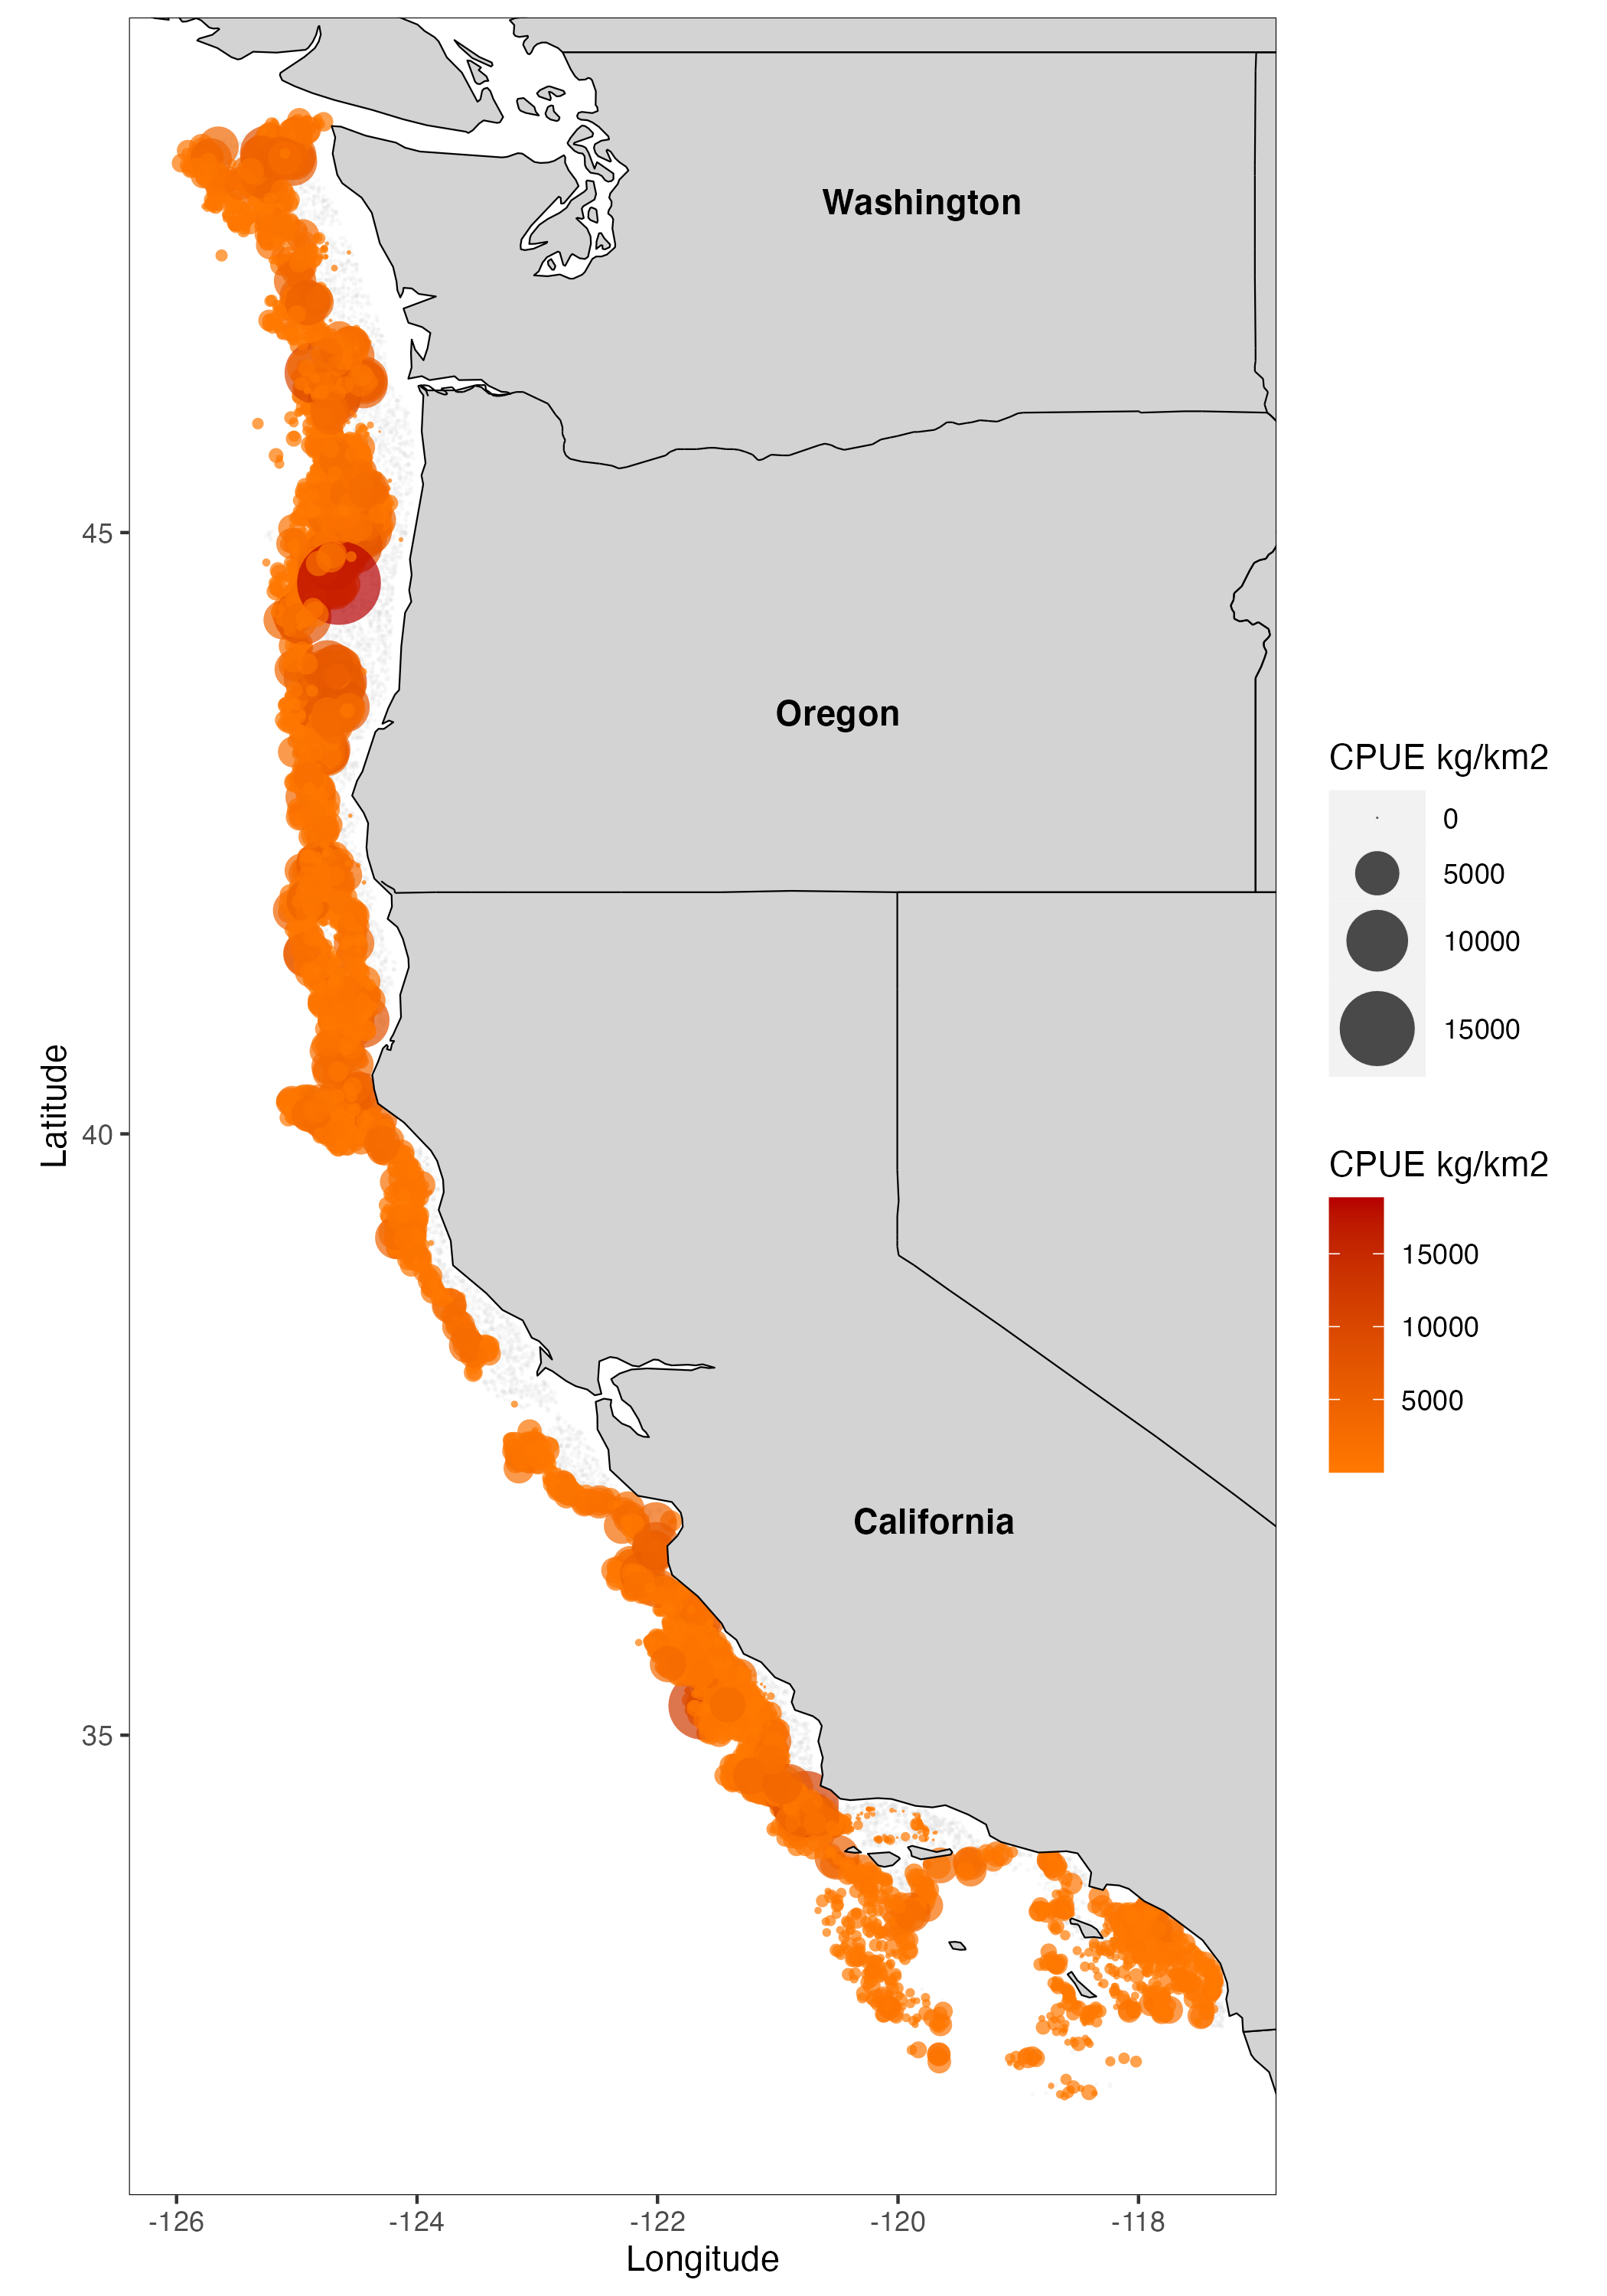
\includegraphics[width=1\textwidth,height=0.75\textheight]{C:/GitHub/Official_shortspine_thornyhead_2023/doc/FinalFigs/Intro/stock-map.png}
\caption{Biomass of shortspine thornyhead found in the NWFSC West Coast Groundfish Bottom Trawl Survey annual survey (2003-2022) coastwide.\label{fig:stock-map}}
\end{figure}

\begin{figure}
\centering
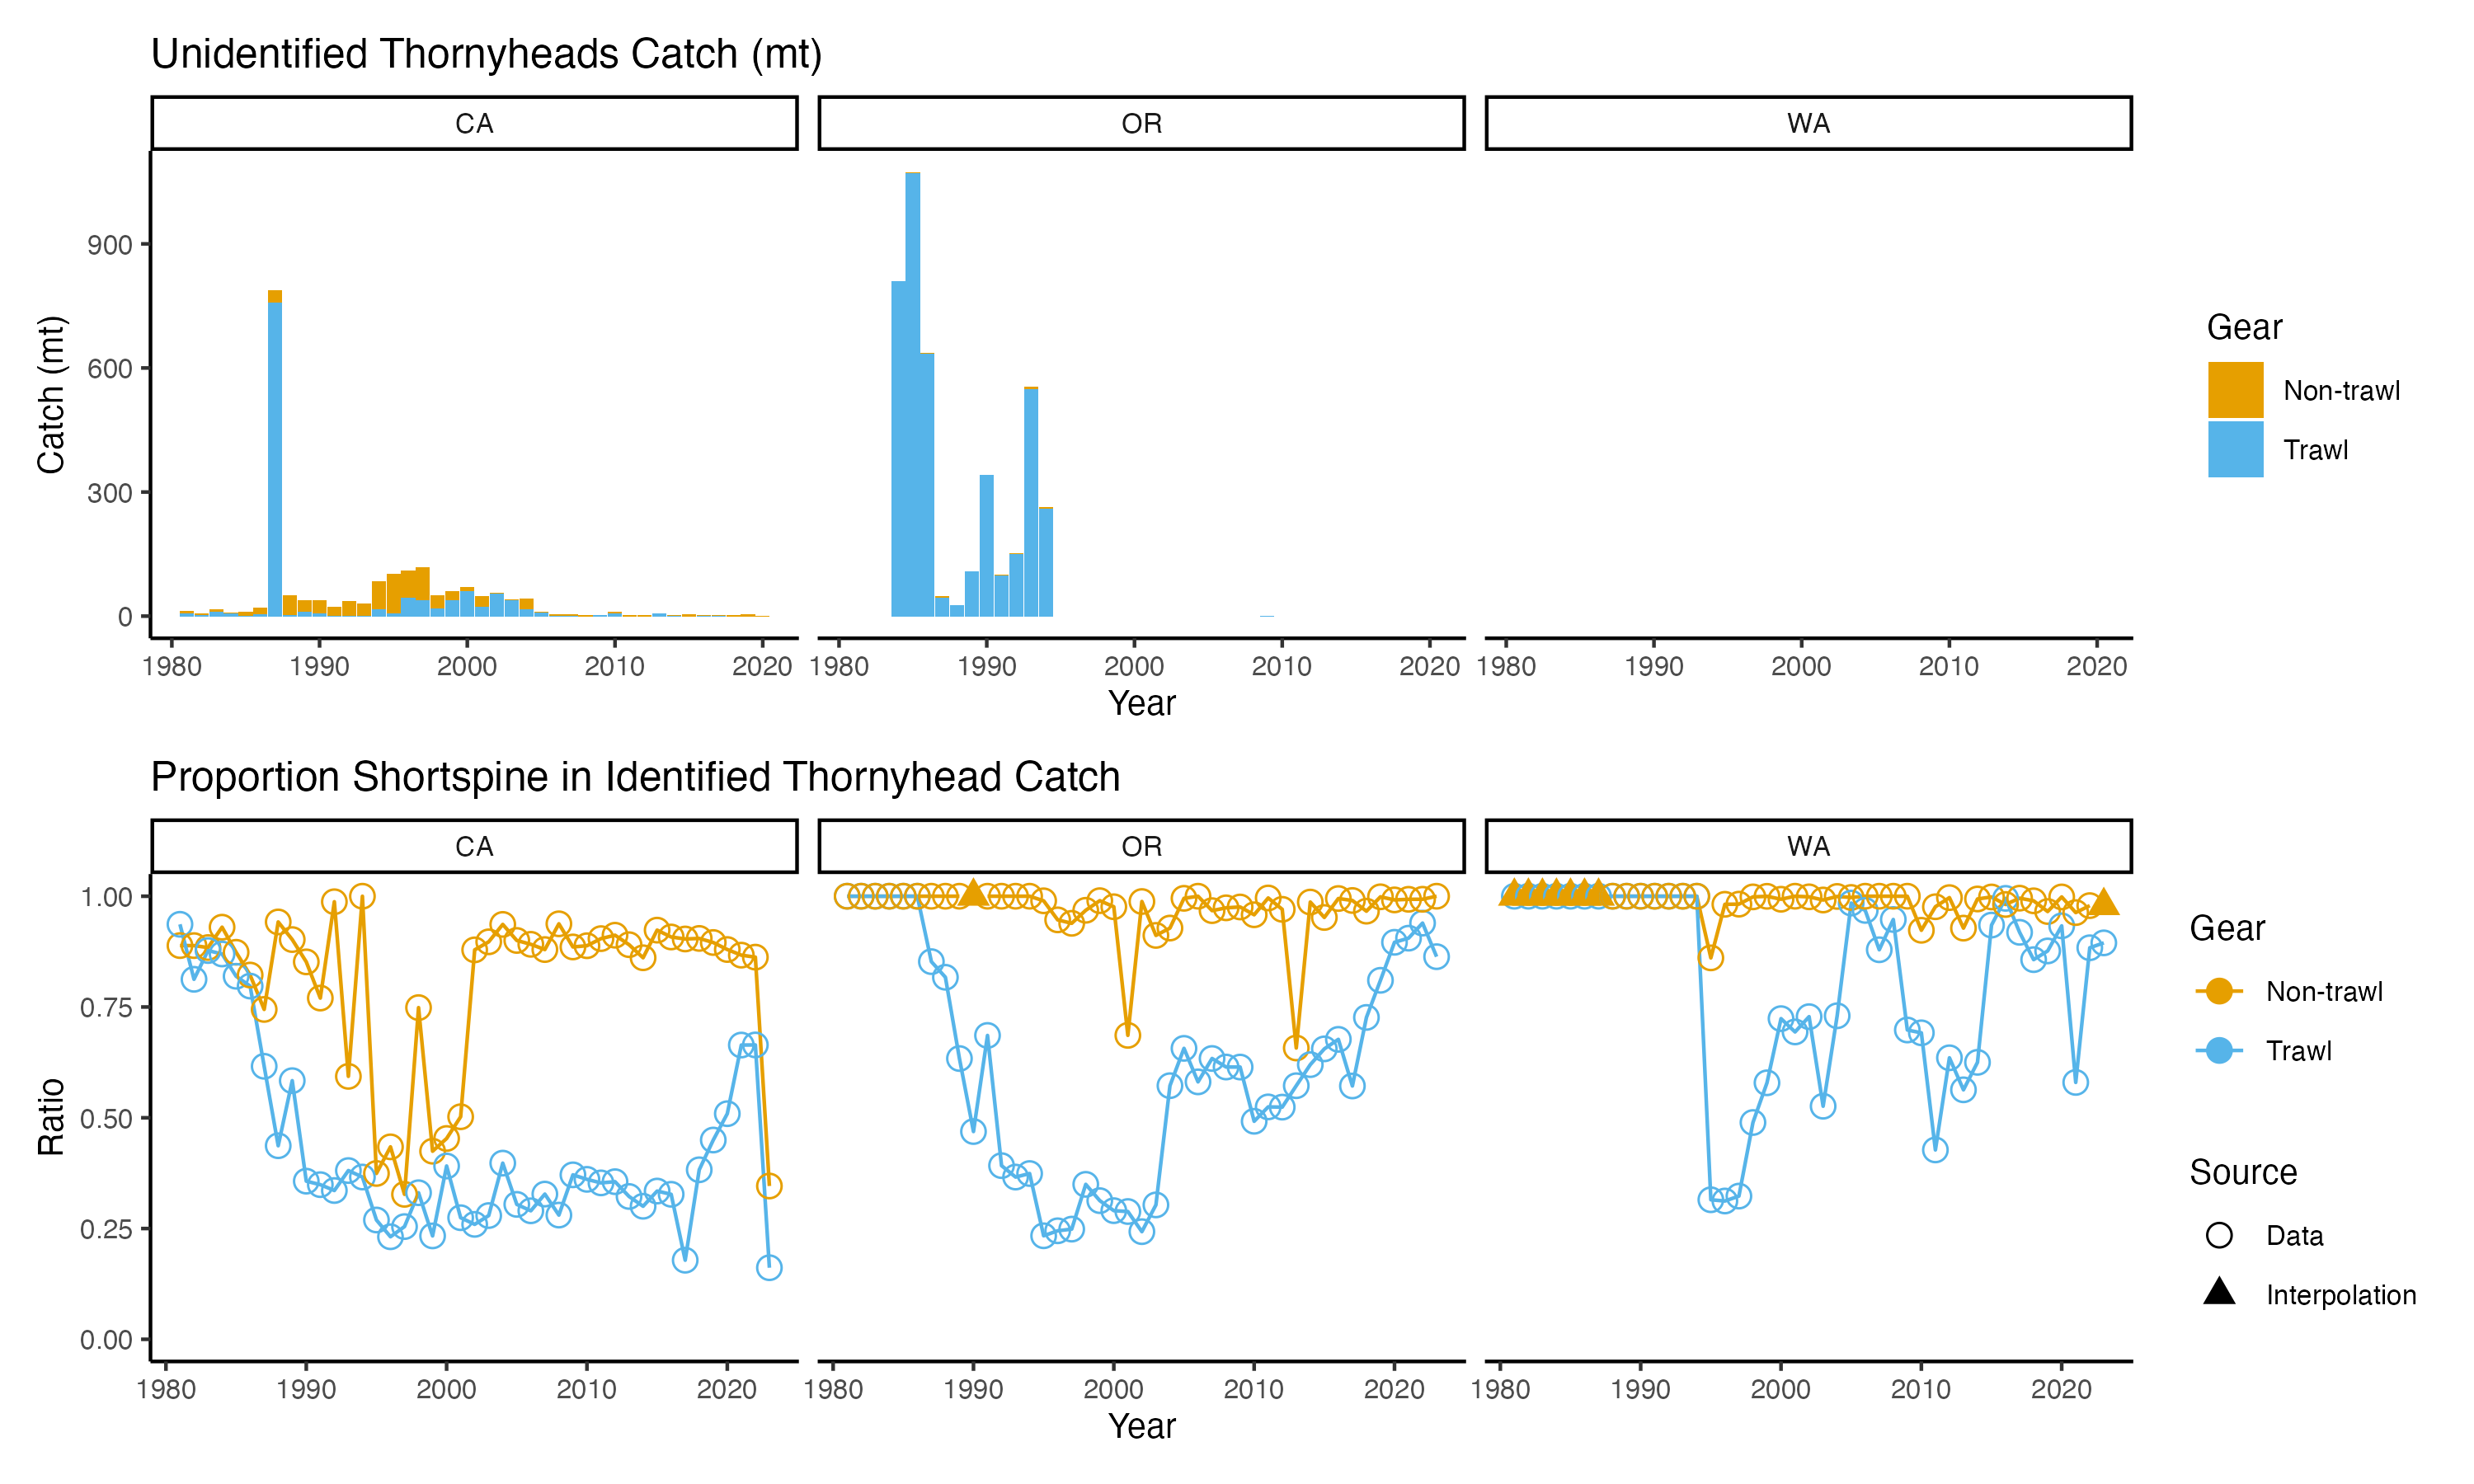
\includegraphics[width=1\textwidth,height=1\textheight]{C:/GitHub/Official_shortspine_thornyhead_2023/doc/FinalFigs/Intro/thornyhead-ratio.png}
\caption{Unidentified thornyhead catches (mt) and the proportion identified as shortspines, calculated as the ratio of shortspine thornyhead catches to combined longspine and shortspine catches.\label{fig:thornyhead-ratio}}
\end{figure}

\begin{figure}
\centering
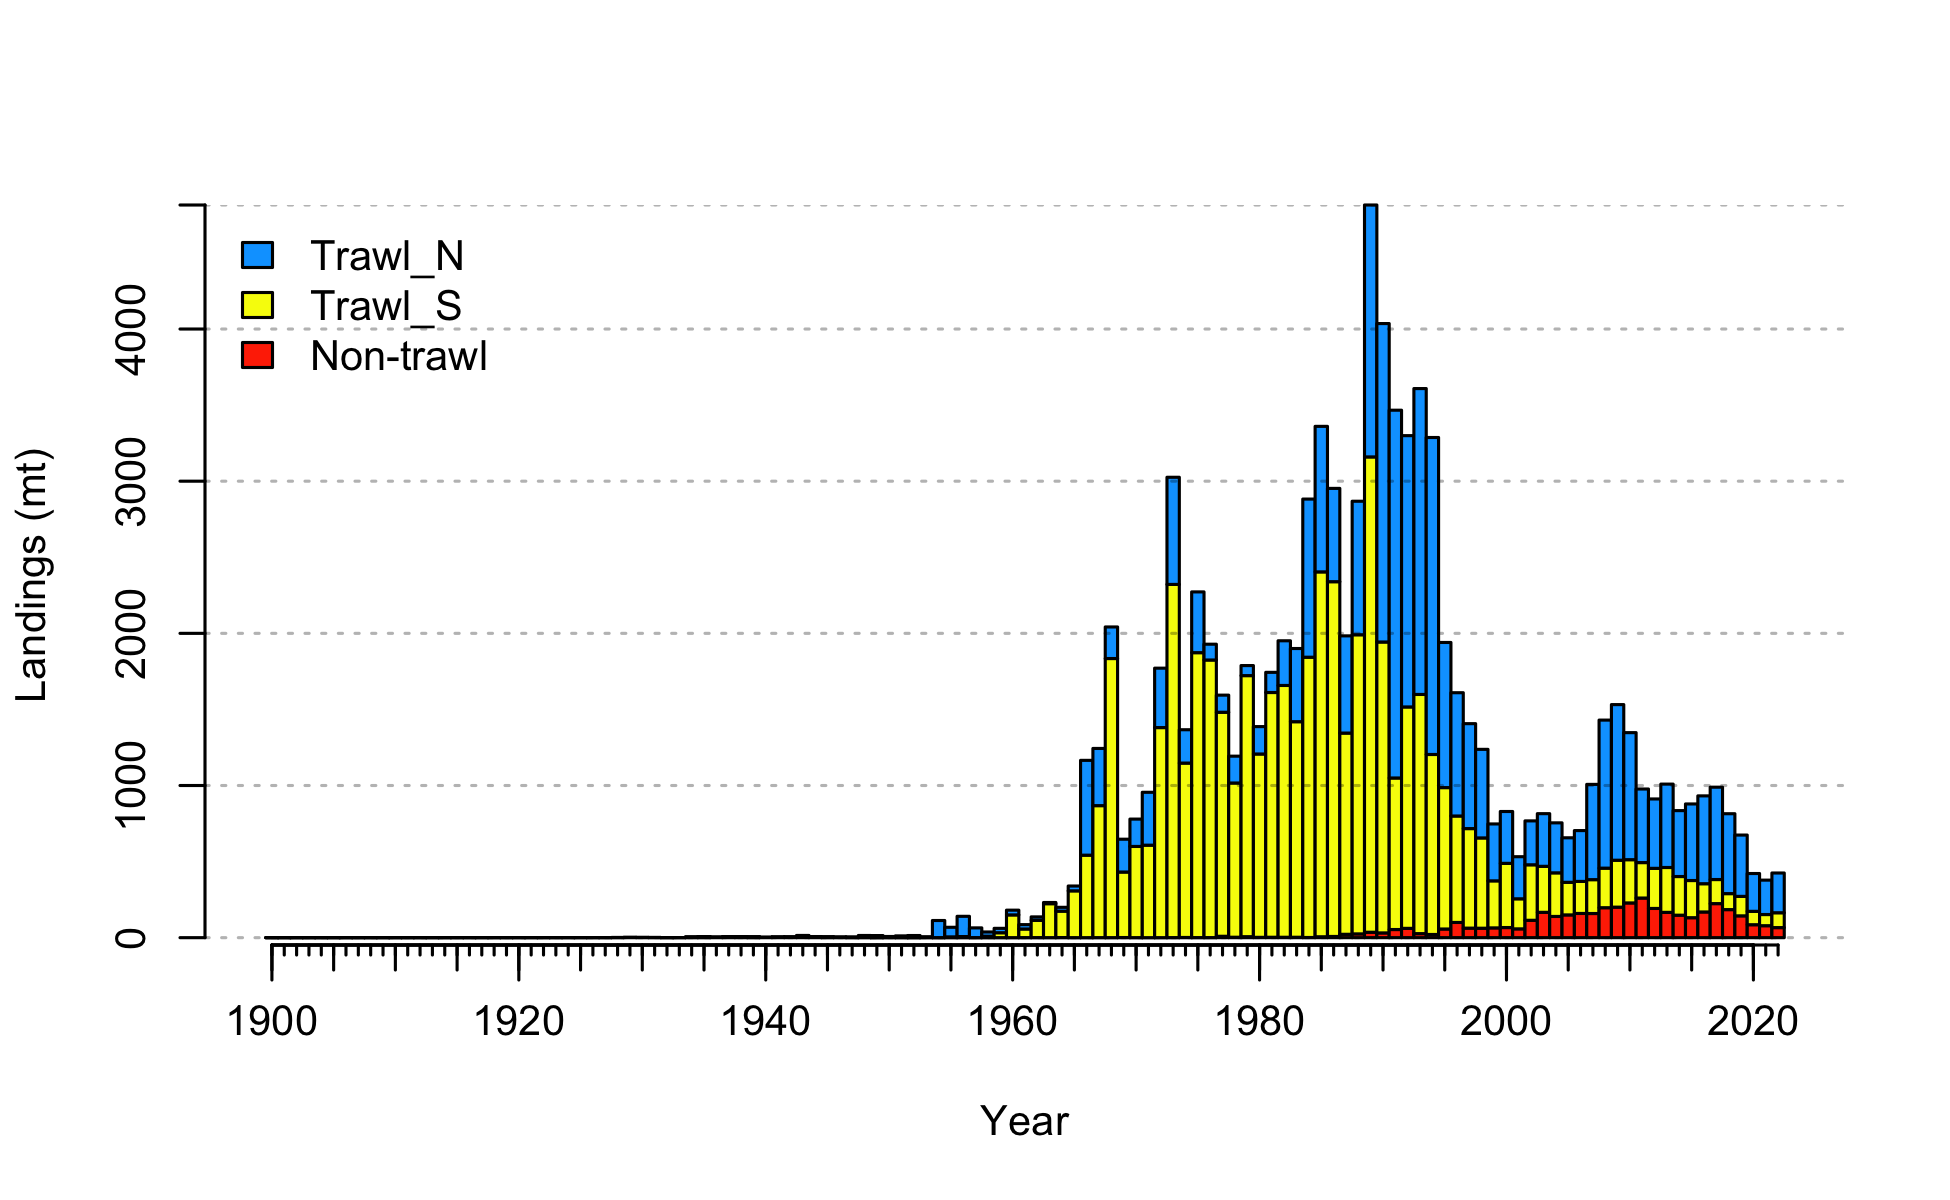
\includegraphics[width=1\textwidth,height=1\textheight]{C:/GitHub/Official_shortspine_thornyhead_2023/doc/FinalFigs/Base/catch2 landings stacked.png}
\caption{Landing history for shortspine thornyhead.\label{fig:catch_hist}}
\end{figure}

\begin{figure}
\centering
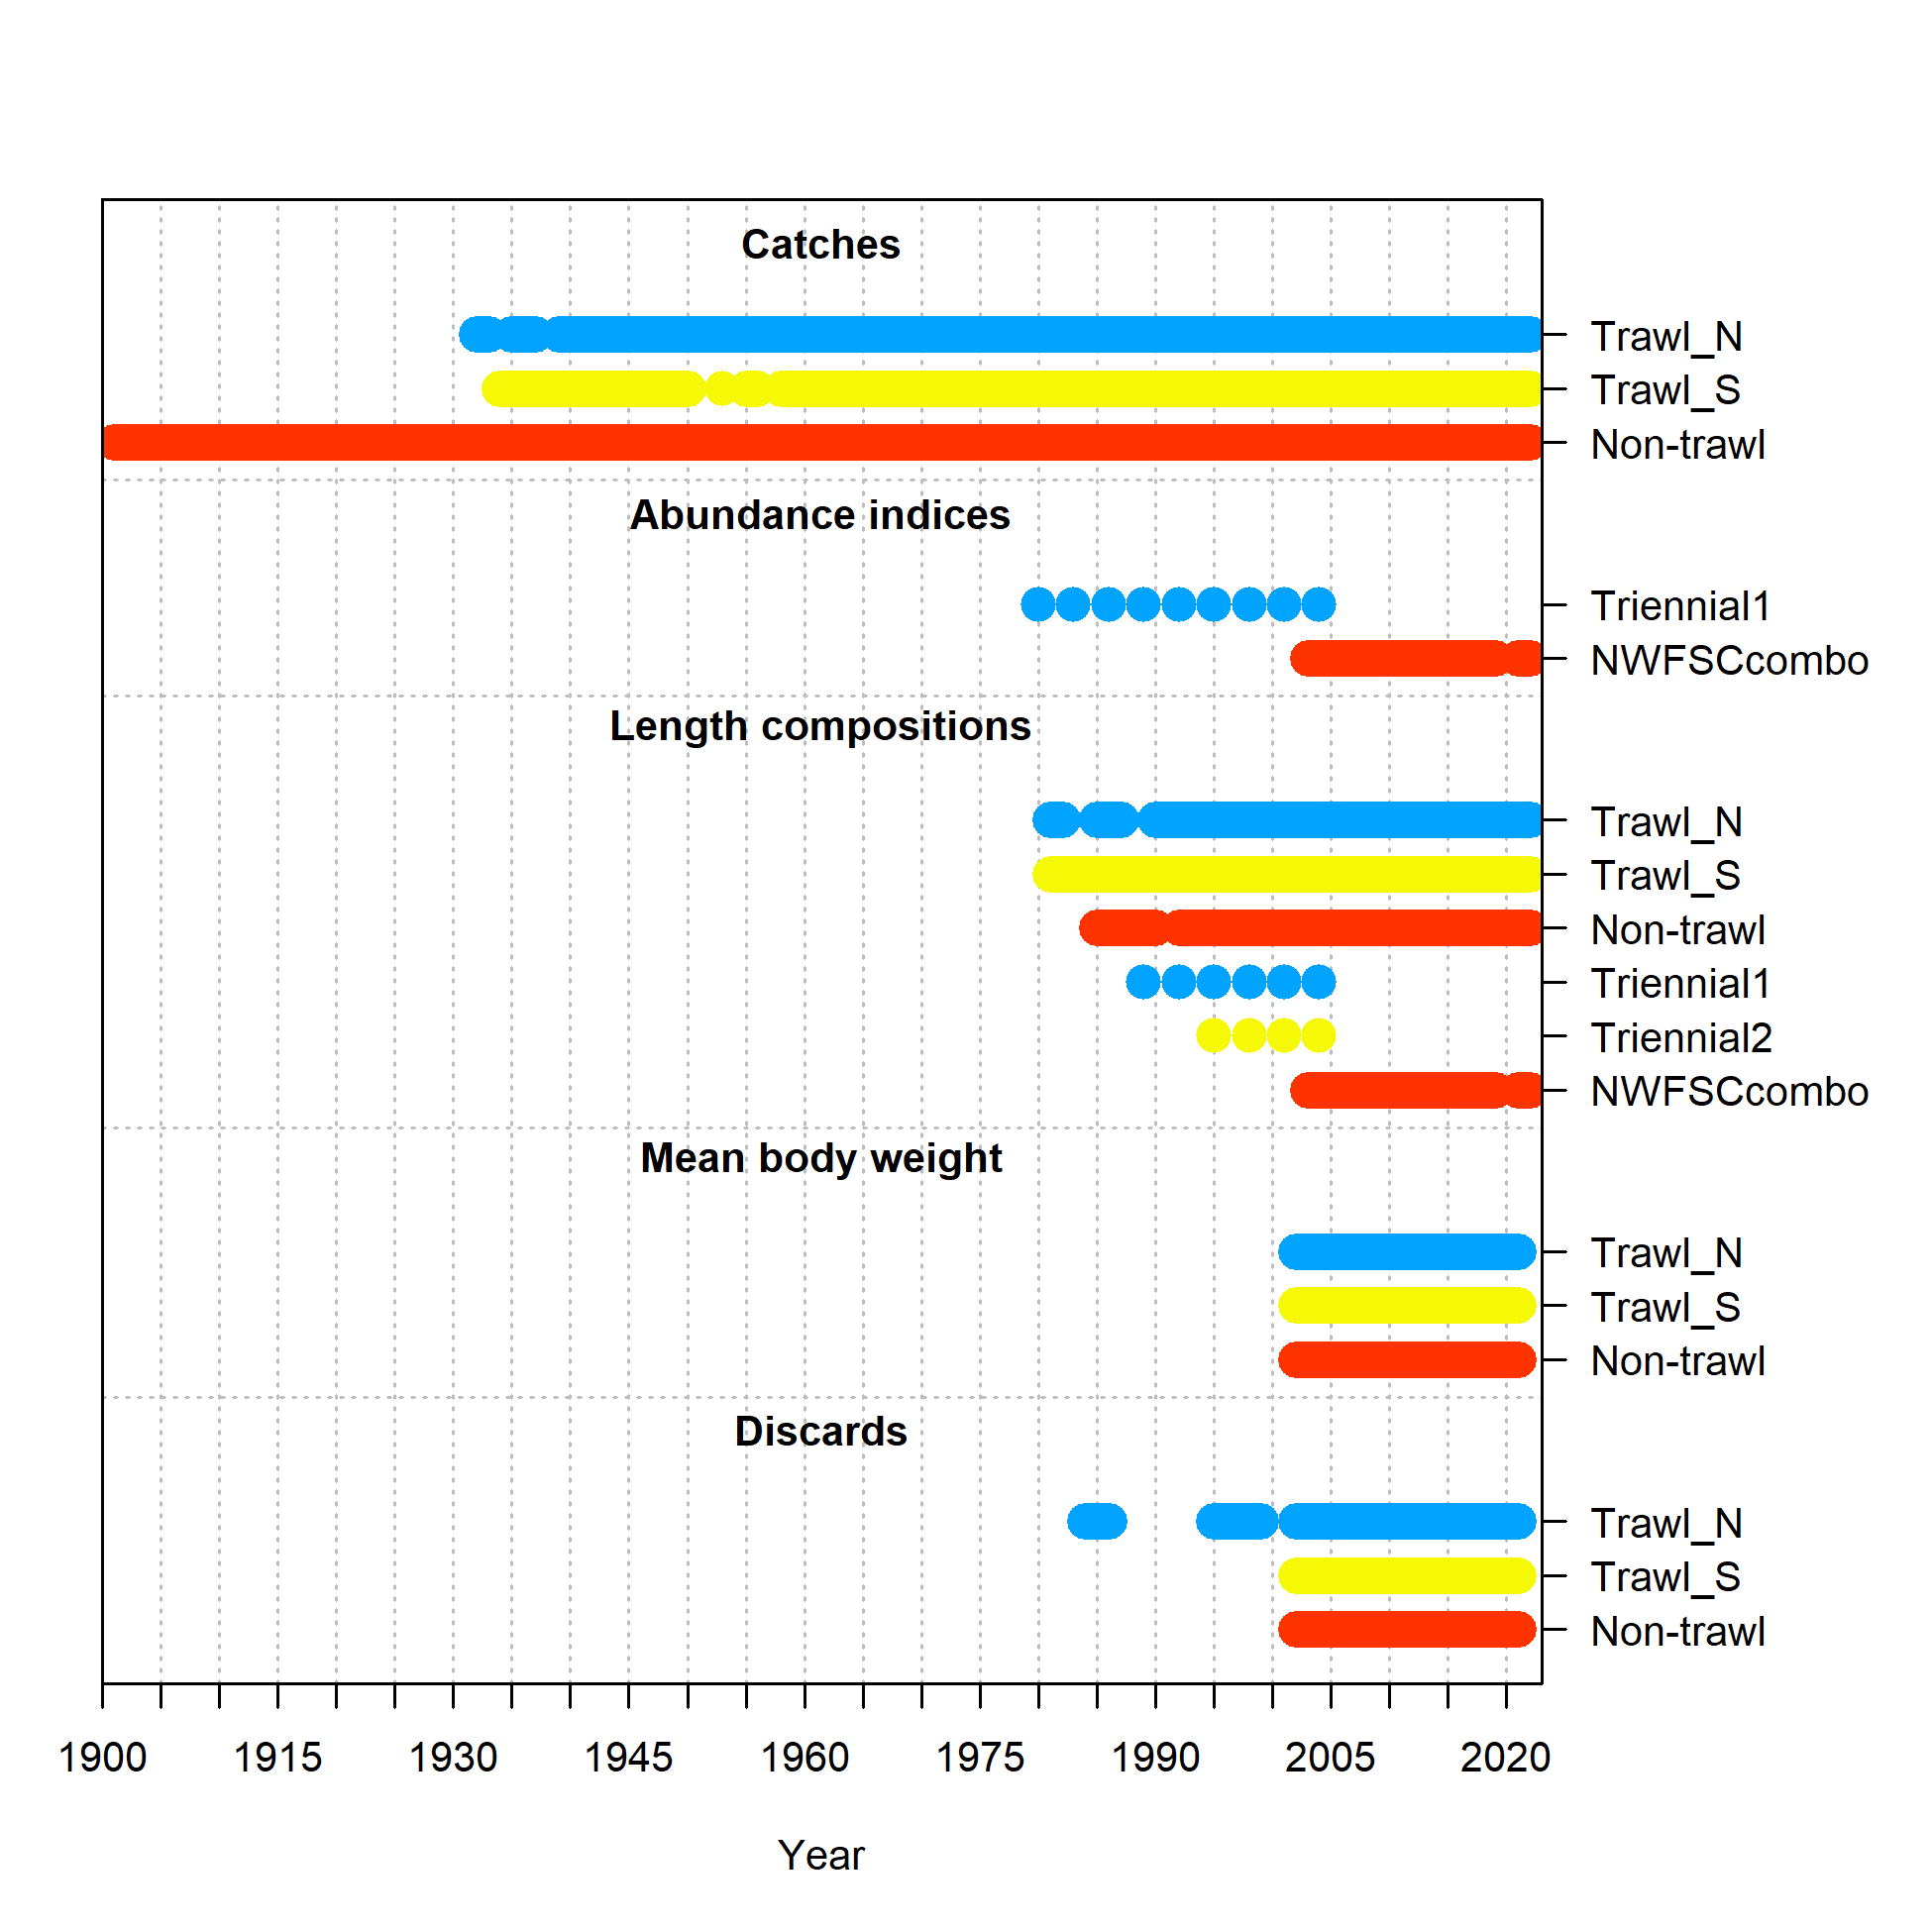
\includegraphics[width=1\textwidth,height=1\textheight]{C:/GitHub/Official_shortspine_thornyhead_2023/doc/FinalFigs/Data/data_plot.png}
\caption{Summary of data sources used in the base model.\label{fig:assessment_data_timeseries}}
\end{figure}

\begin{figure}
\centering
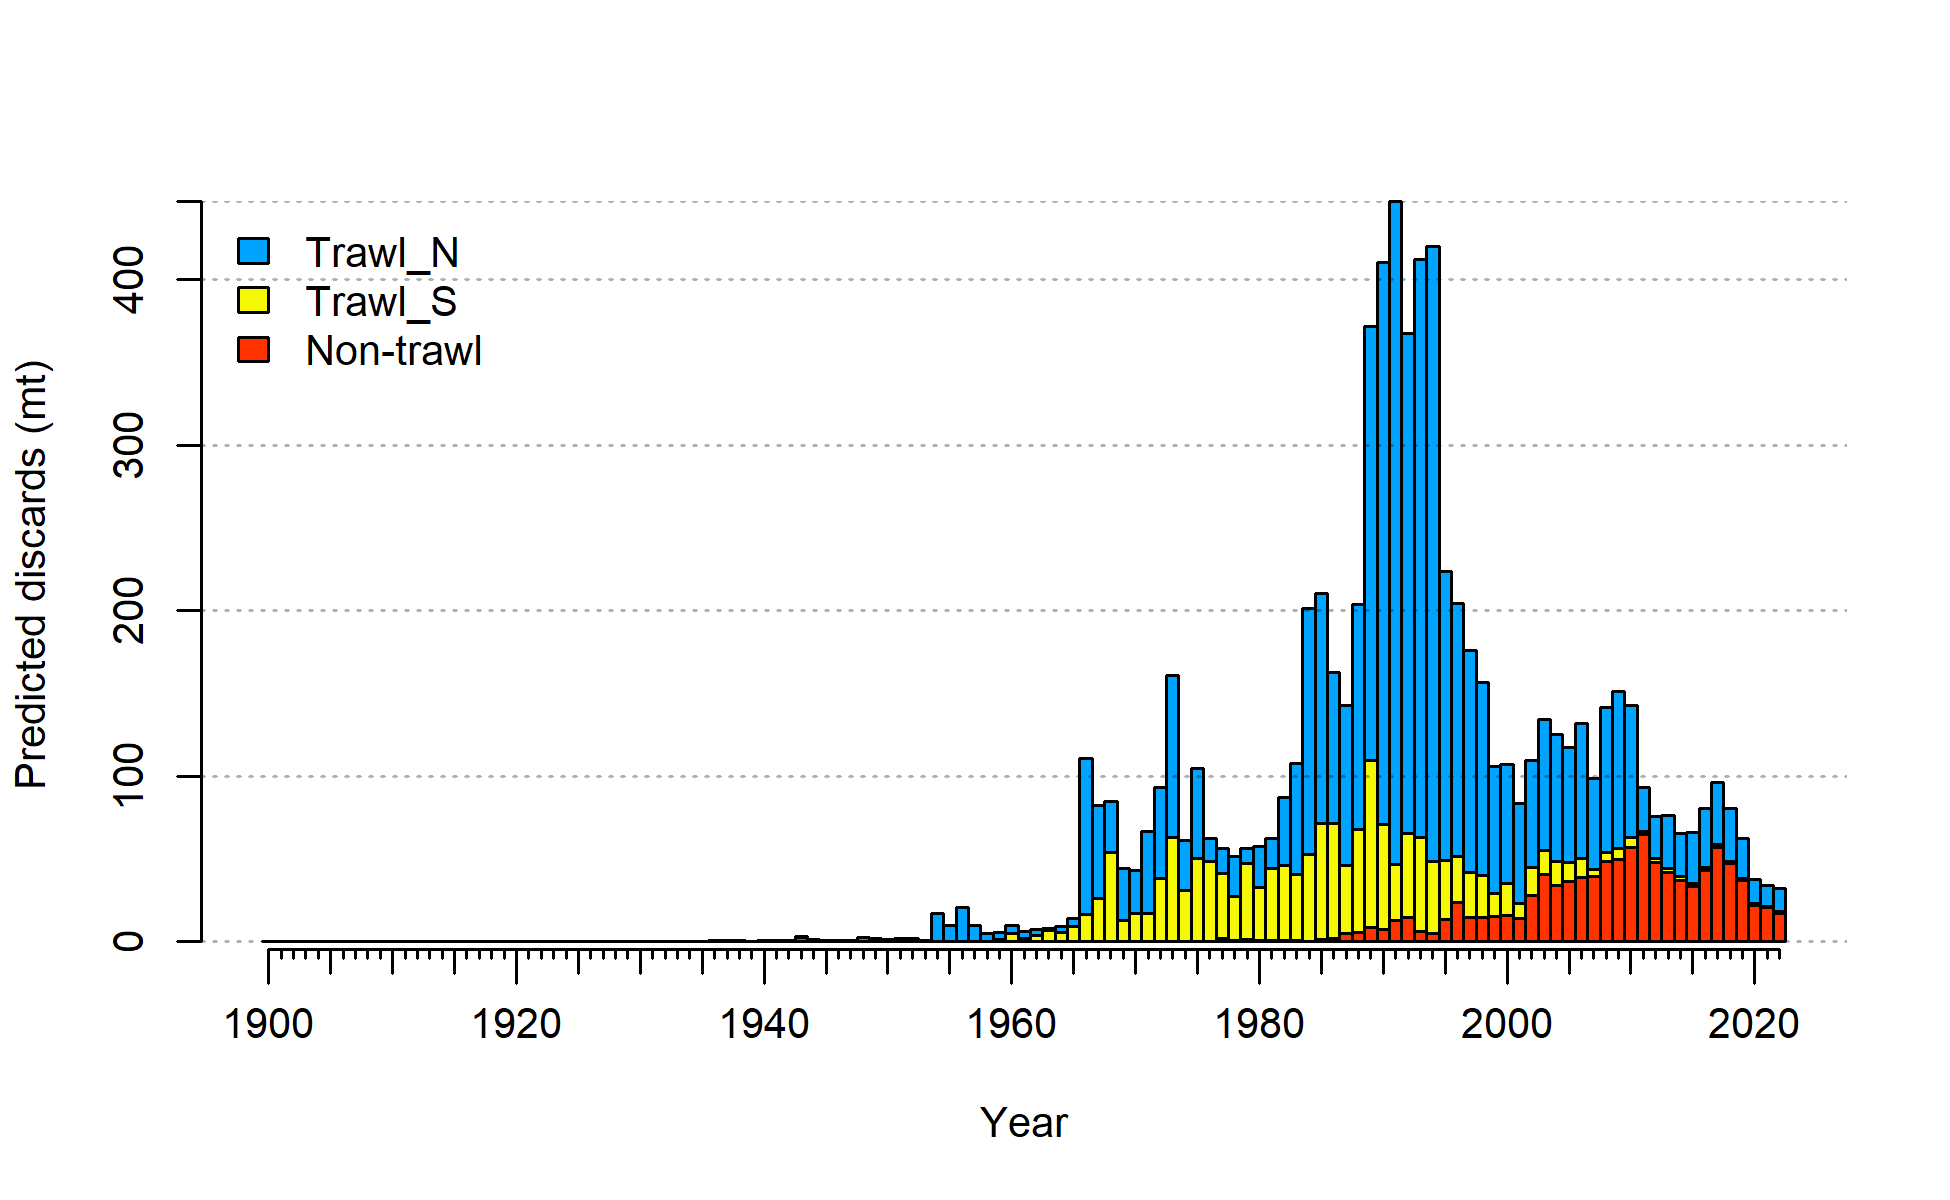
\includegraphics[width=1\textwidth,height=1\textheight]{C:/GitHub/Official_shortspine_thornyhead_2023/doc/FinalFigs/Base/catch7 discards stacked plot (depends on multiple fleets).png}
\caption{Predicted discards based estimated retention and selectivity for each fleet.\label{fig:disc_hist}}
\end{figure}

\begin{figure}
\centering
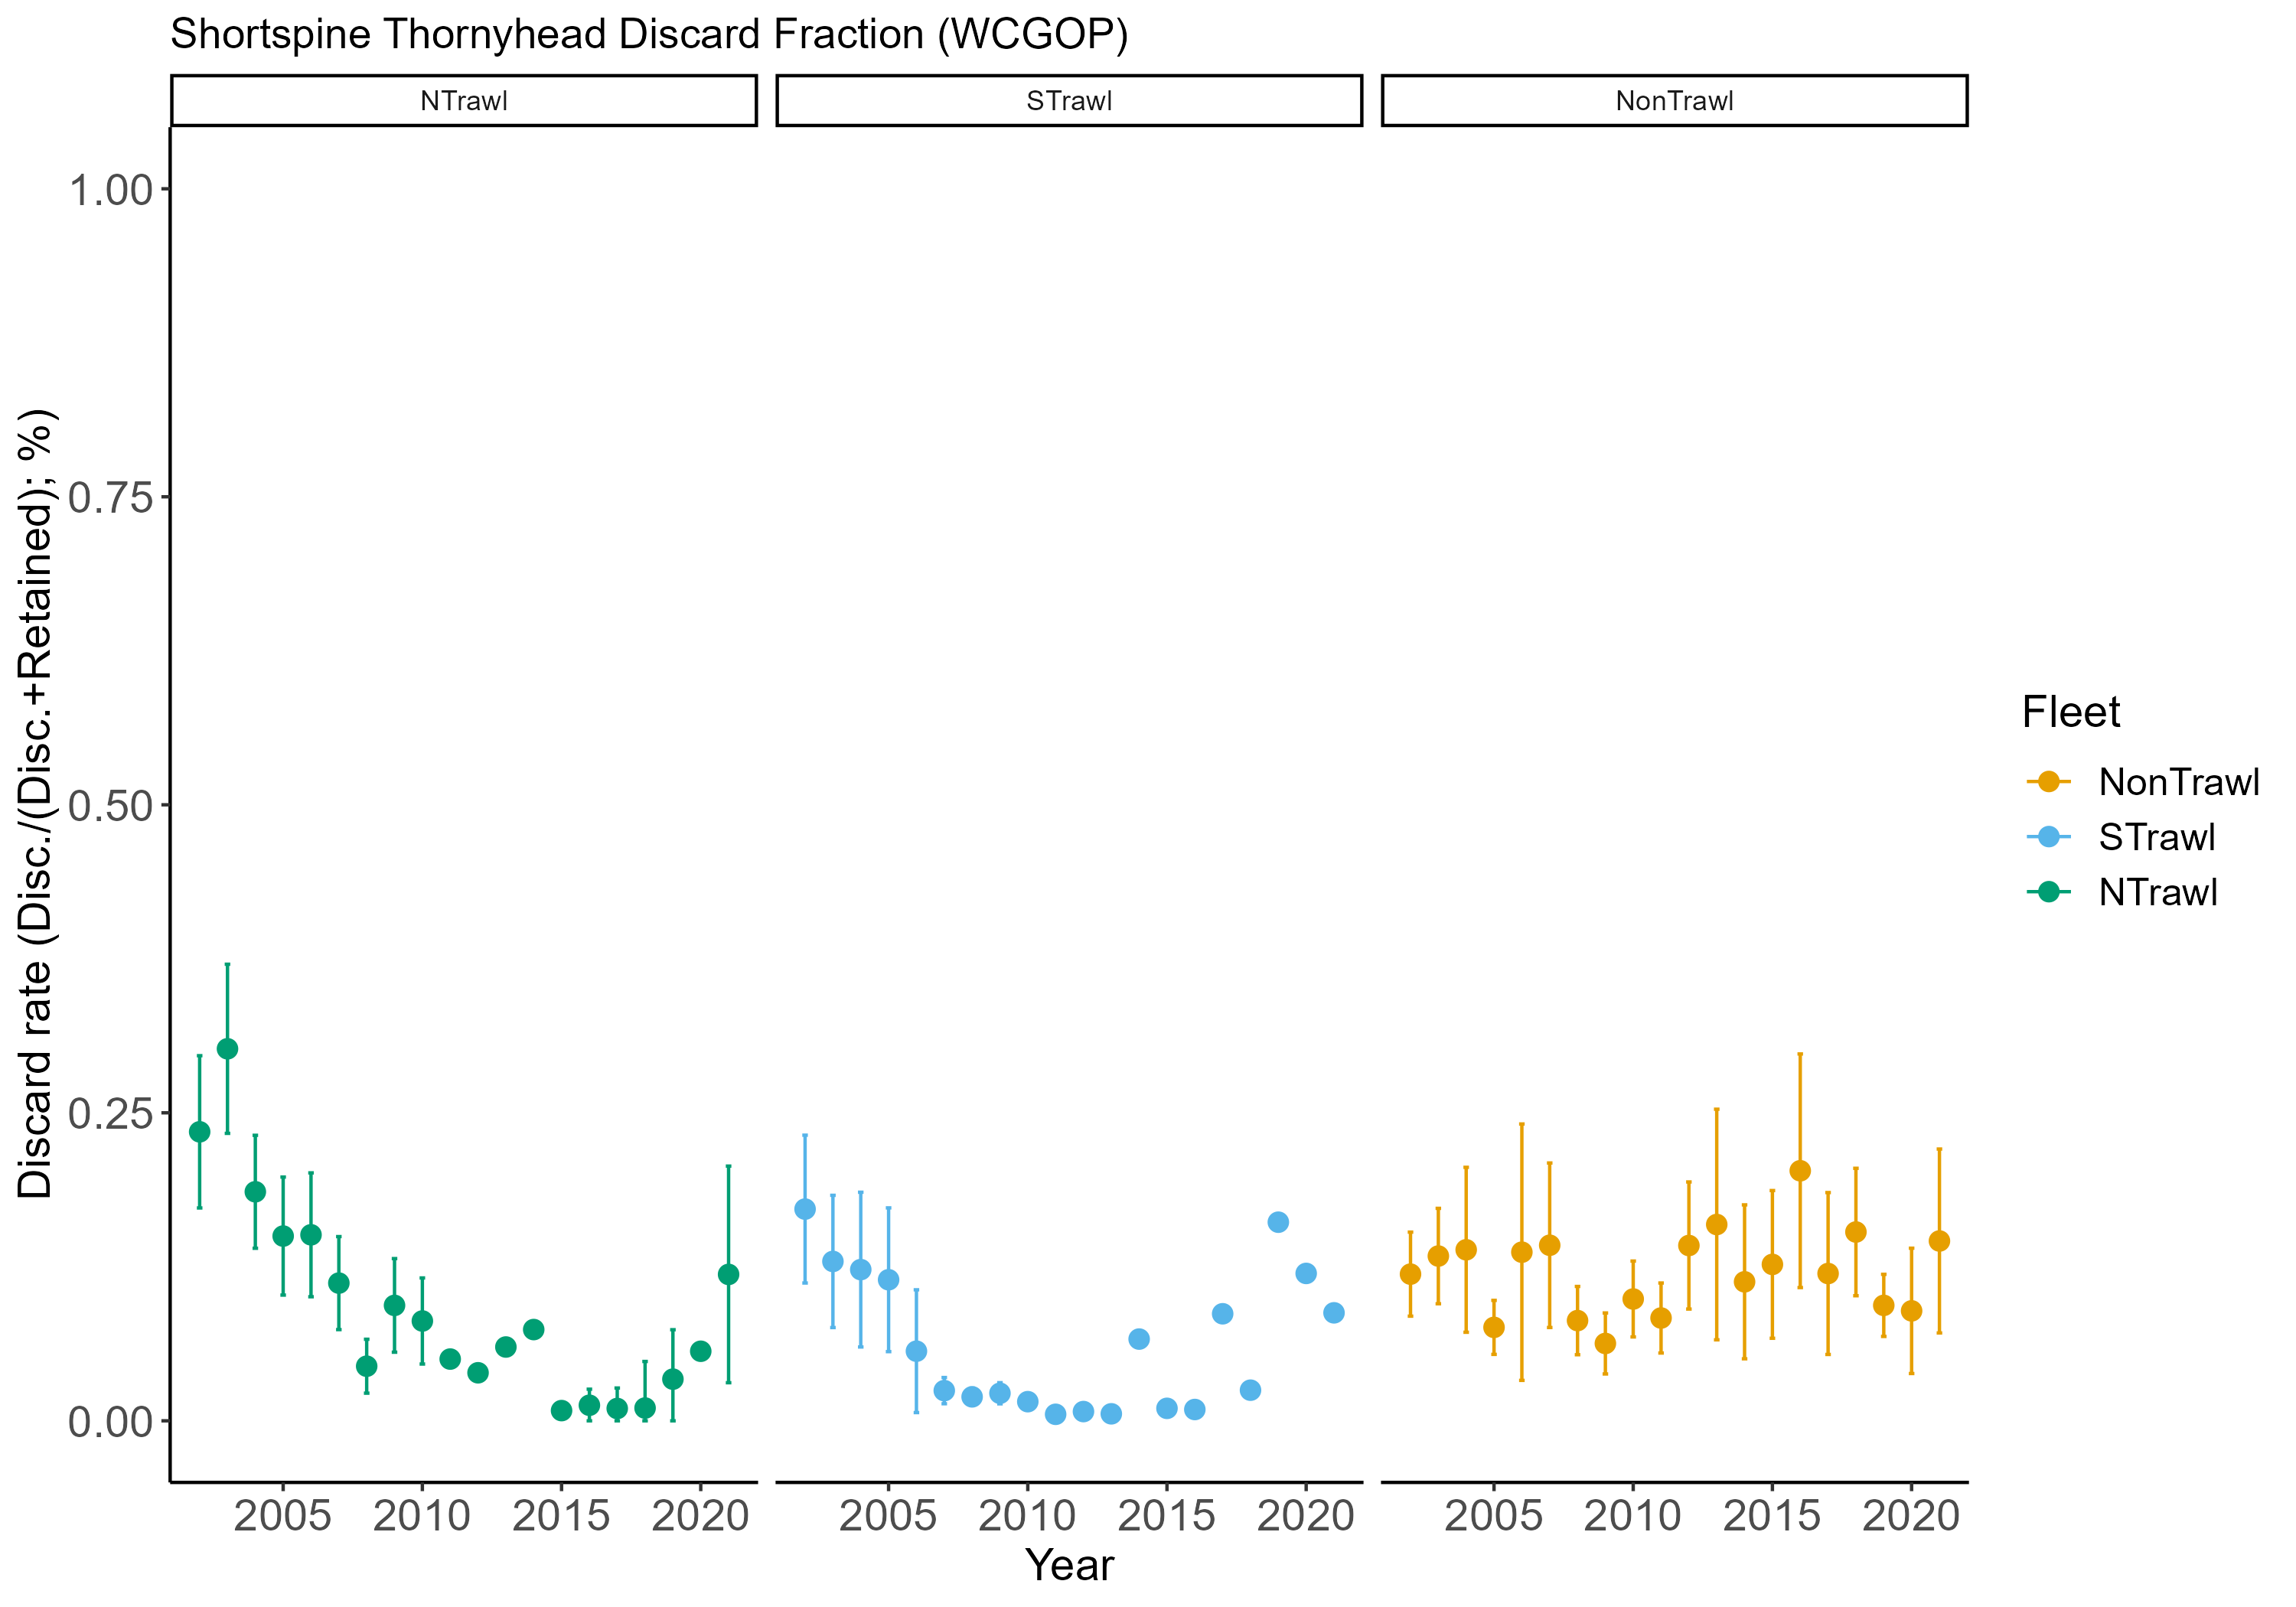
\includegraphics[width=1\textwidth,height=1\textheight]{C:/GitHub/Official_shortspine_thornyhead_2023/doc/FinalFigs/Data/SST_WCGOP_GEMM_discard_rates_3fleet.png}
\caption{Discard rates from the WCGOP data set with catch share and non-catch share considerations from the GEMM dataset.\label{fig:disc_rates_WCGOP}}
\end{figure}

\begin{figure}
\centering
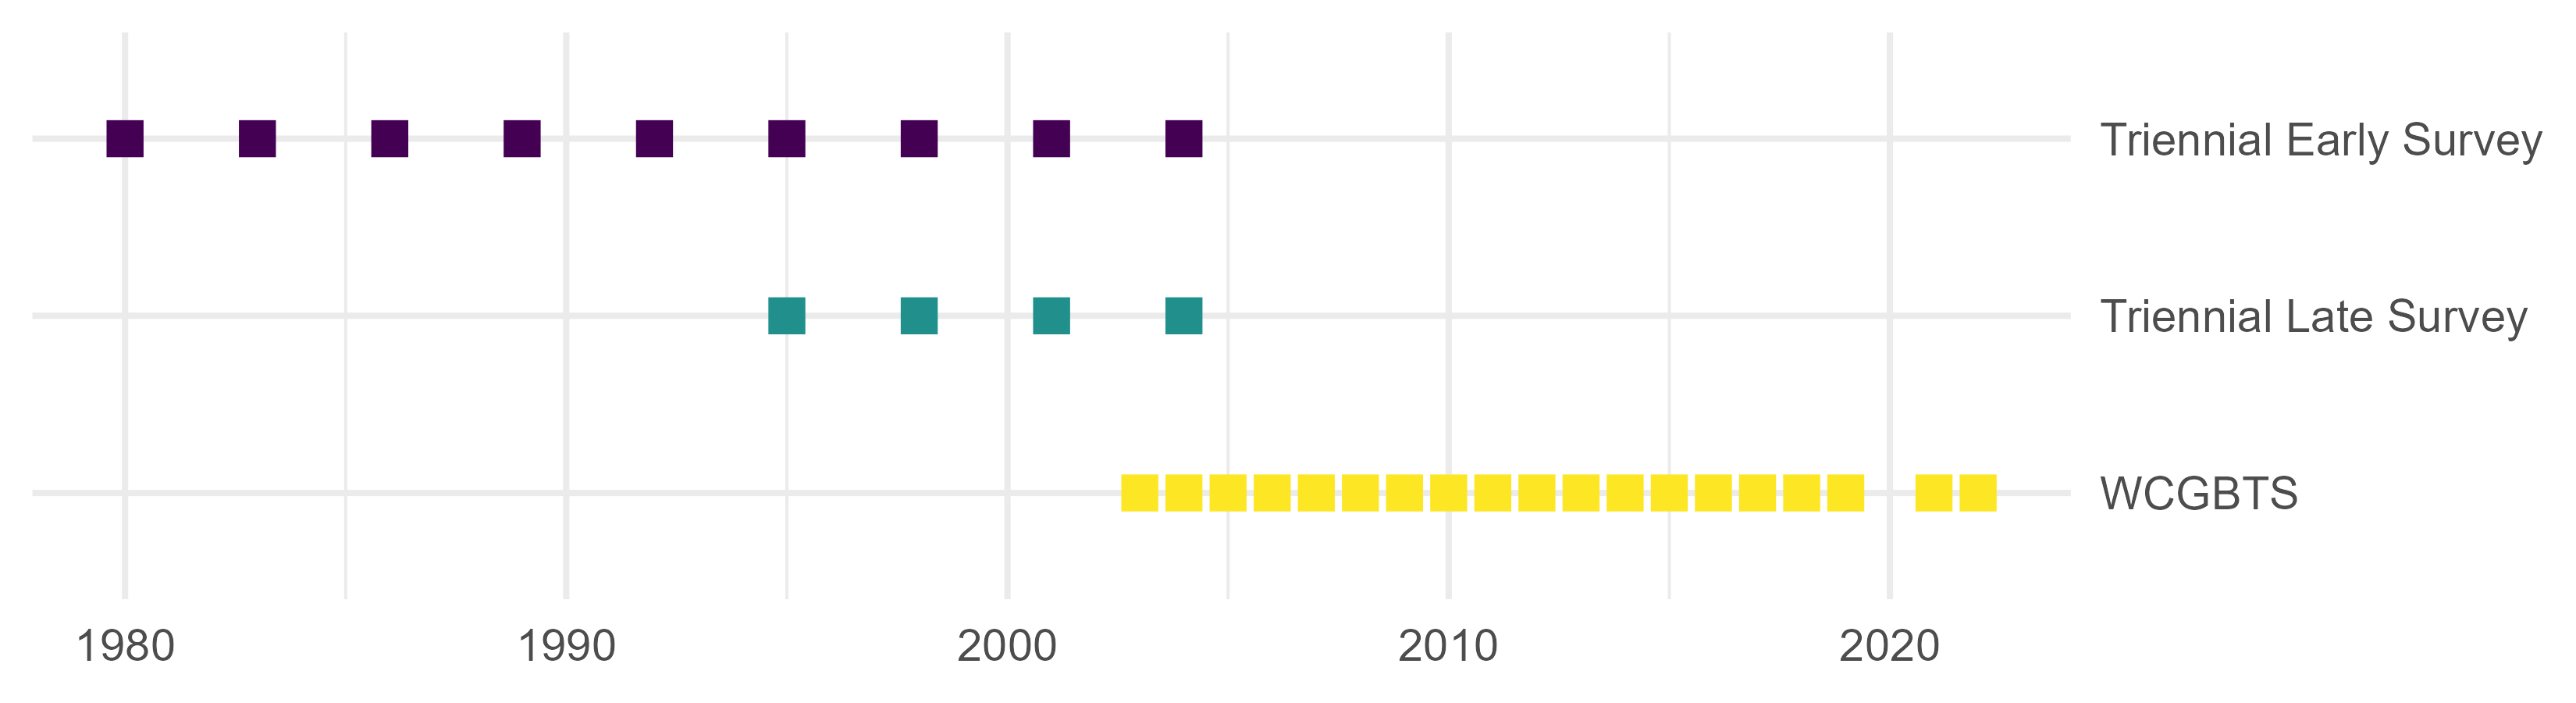
\includegraphics[width=1\textwidth,height=1\textheight]{C:/GitHub/Official_shortspine_thornyhead_2023/doc/FinalFigs/Data/survey_data_timeseries.png}
\caption{Summary of survey data sources used in the base model.\label{fig:survey_data_timeseries}}
\end{figure}

\begin{figure}
\centering
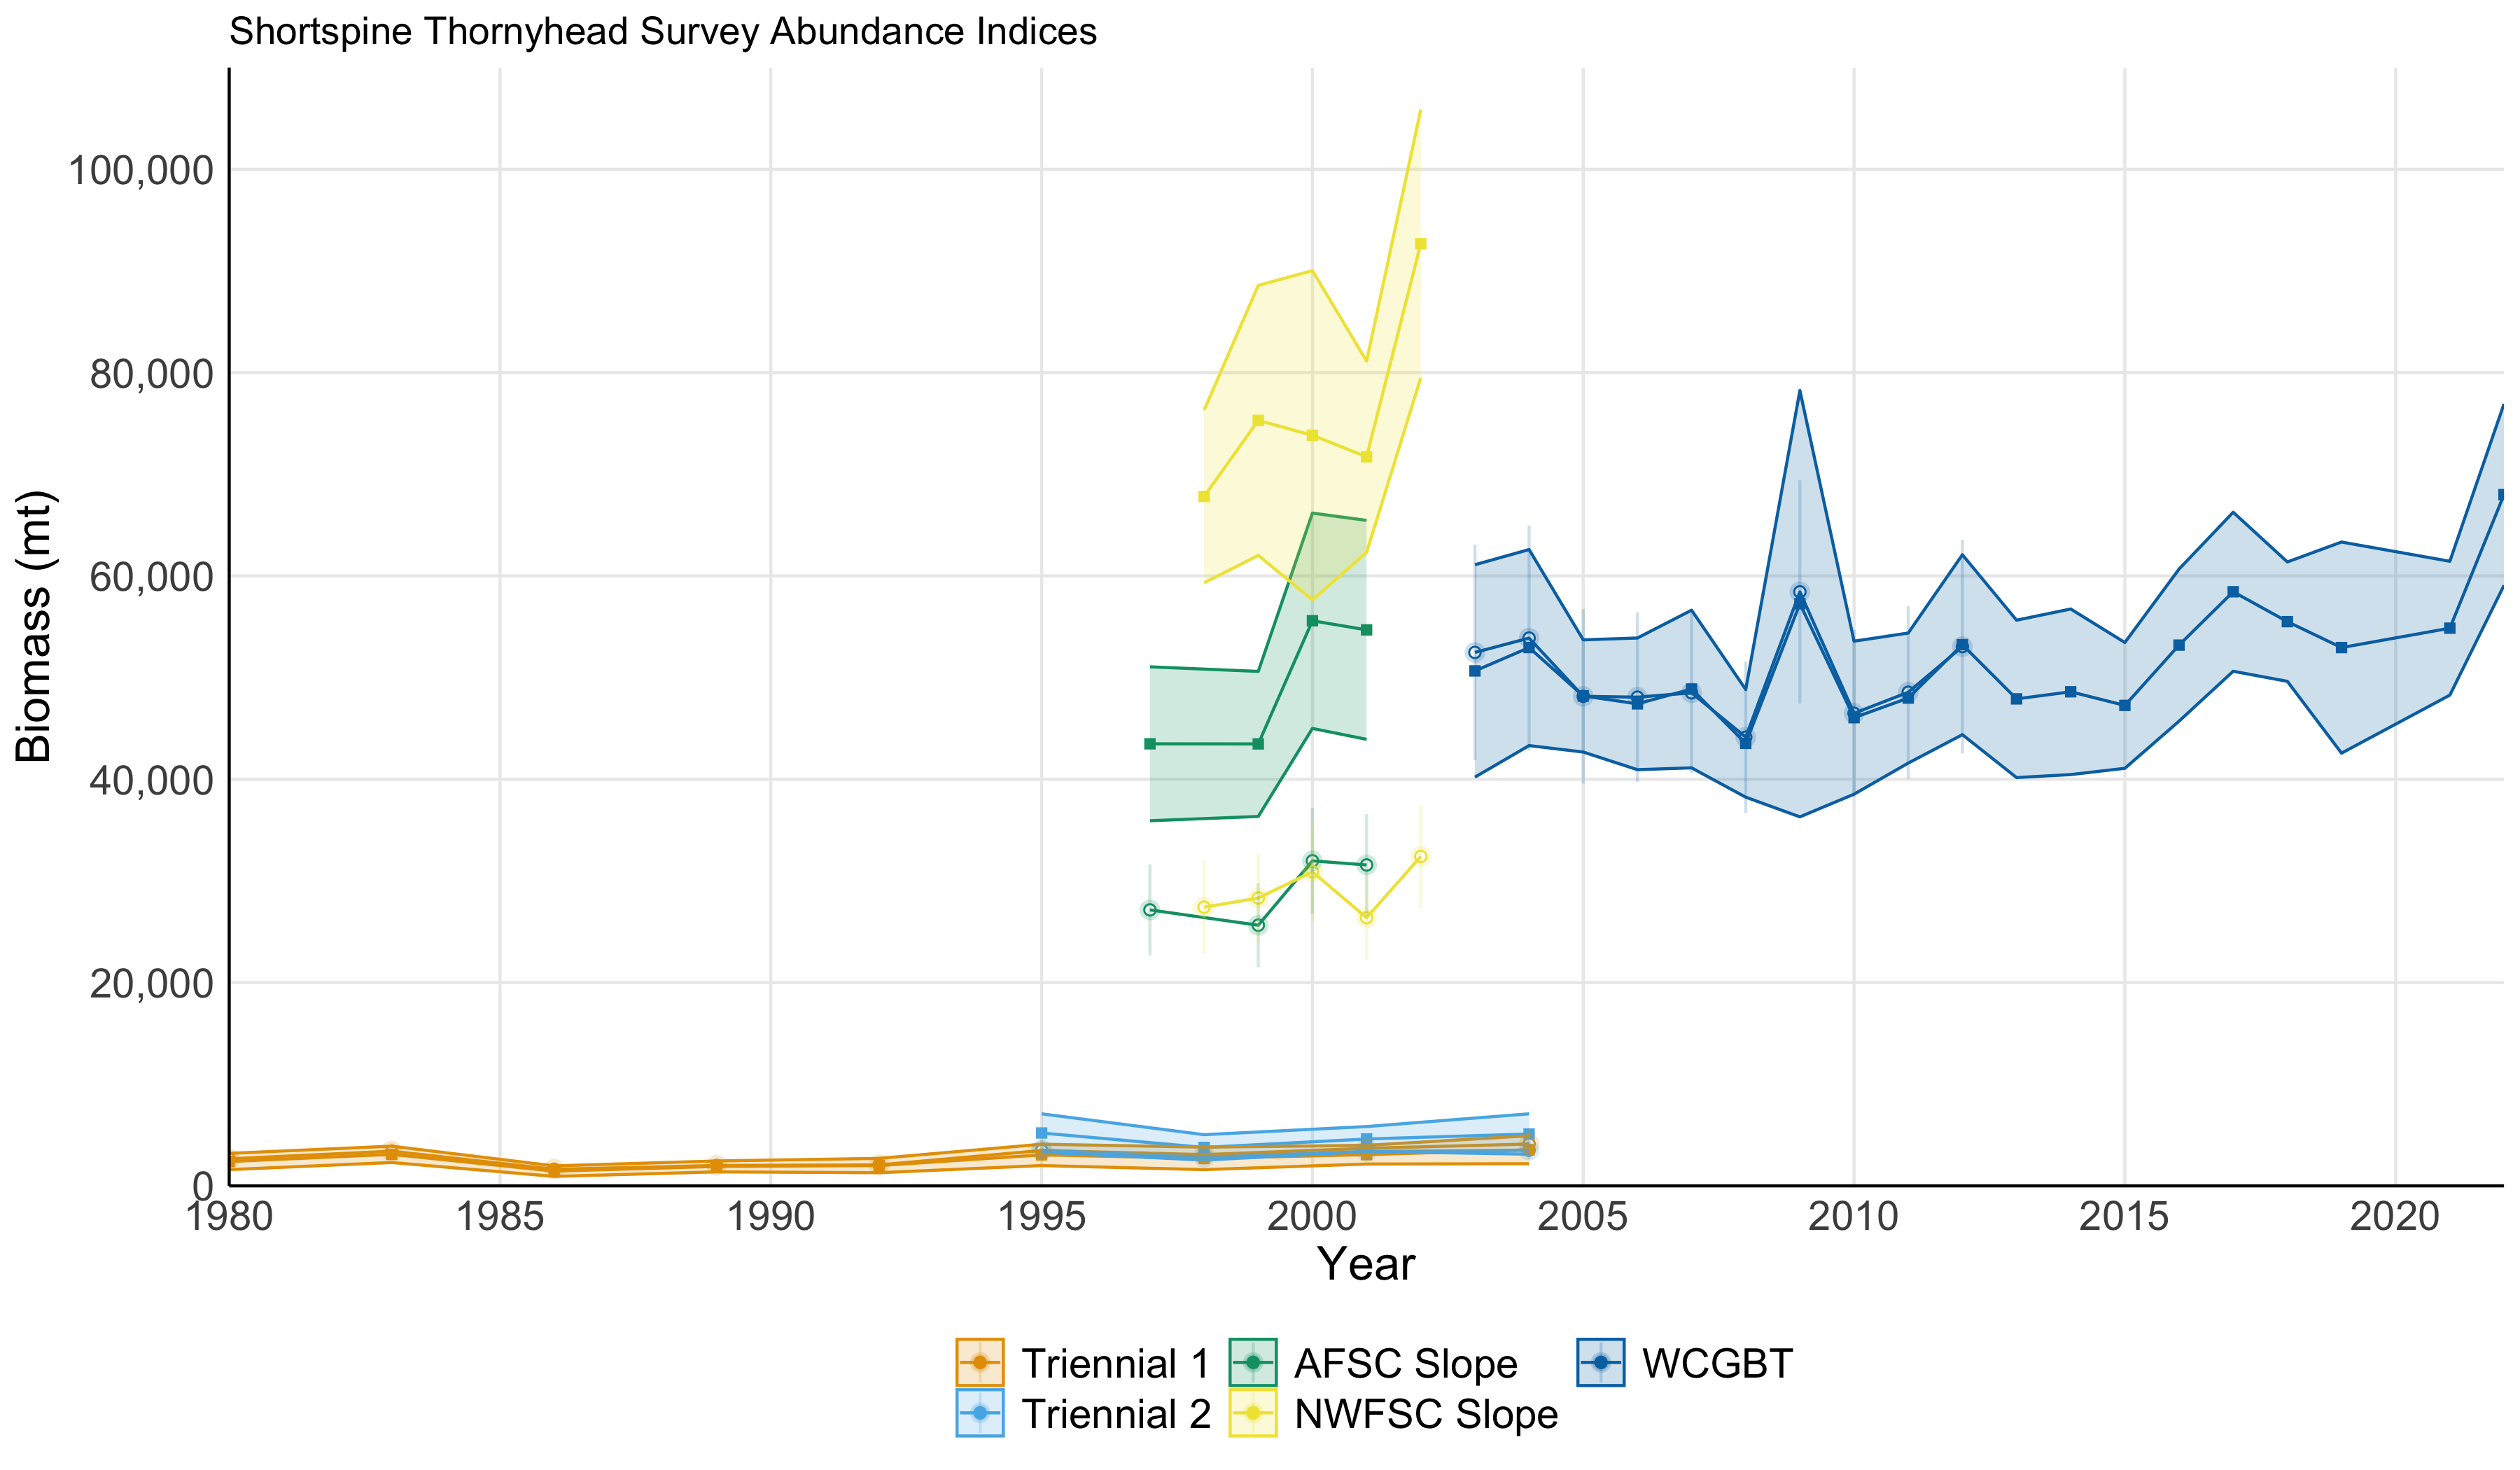
\includegraphics[width=1\textwidth,height=1\textheight]{C:/GitHub/Official_shortspine_thornyhead_2023/doc/FinalFigs/Data/2013_2023_survey_indices_comparison.png}
\caption{Abundance index timeseries. Points with shaded regions were calculated with survey data through 2023 using the \texttt{nwfscSurvey} R package, while points with errorbars are taken directly from the 2013 assessment which used GLMs.\label{fig:designbasedsurv}}
\end{figure}

\begin{figure}
\centering
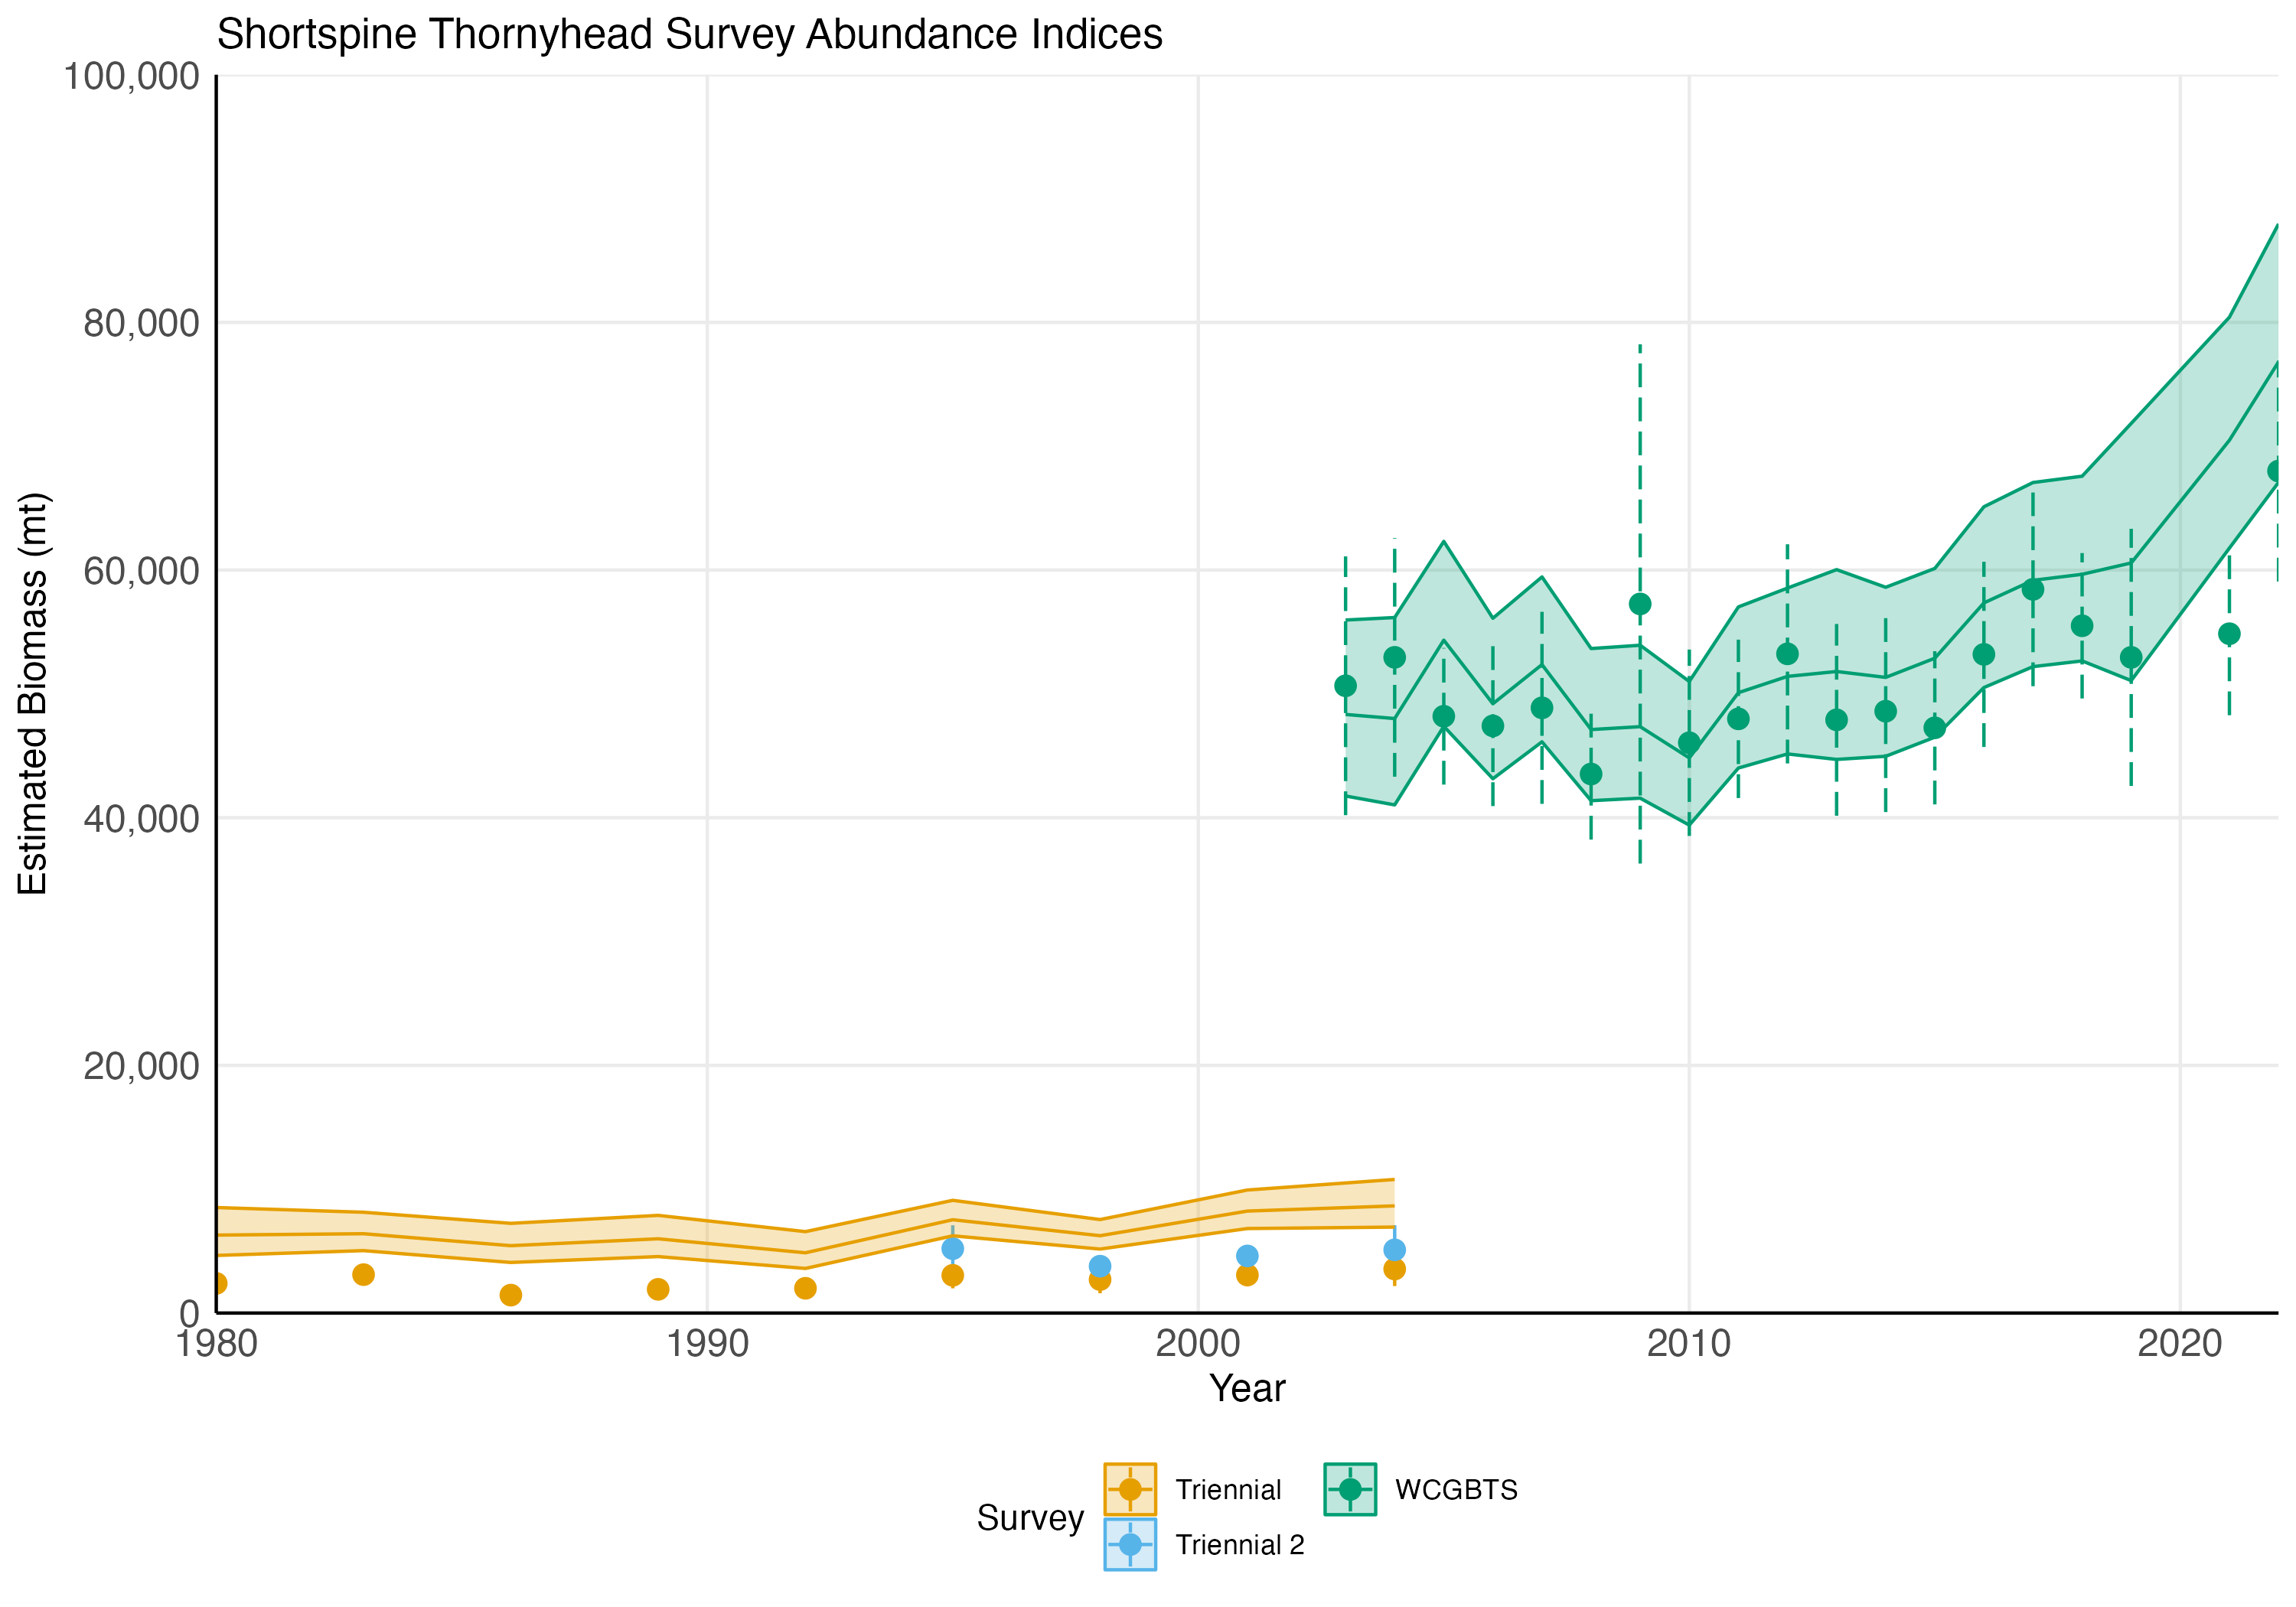
\includegraphics[width=1\textwidth,height=1\textheight]{C:/GitHub/Official_shortspine_thornyhead_2023/doc/FinalFigs/Data/geostat_db_comp_wgcbts_tri.png}
\caption{Abundance index timeseries. Points with shaded regions are the derived from geostatistical models, while points with errorbars are derived from design-based calculations.\label{fig:modelbasedsurv}}
\end{figure}

\begin{figure}
\centering
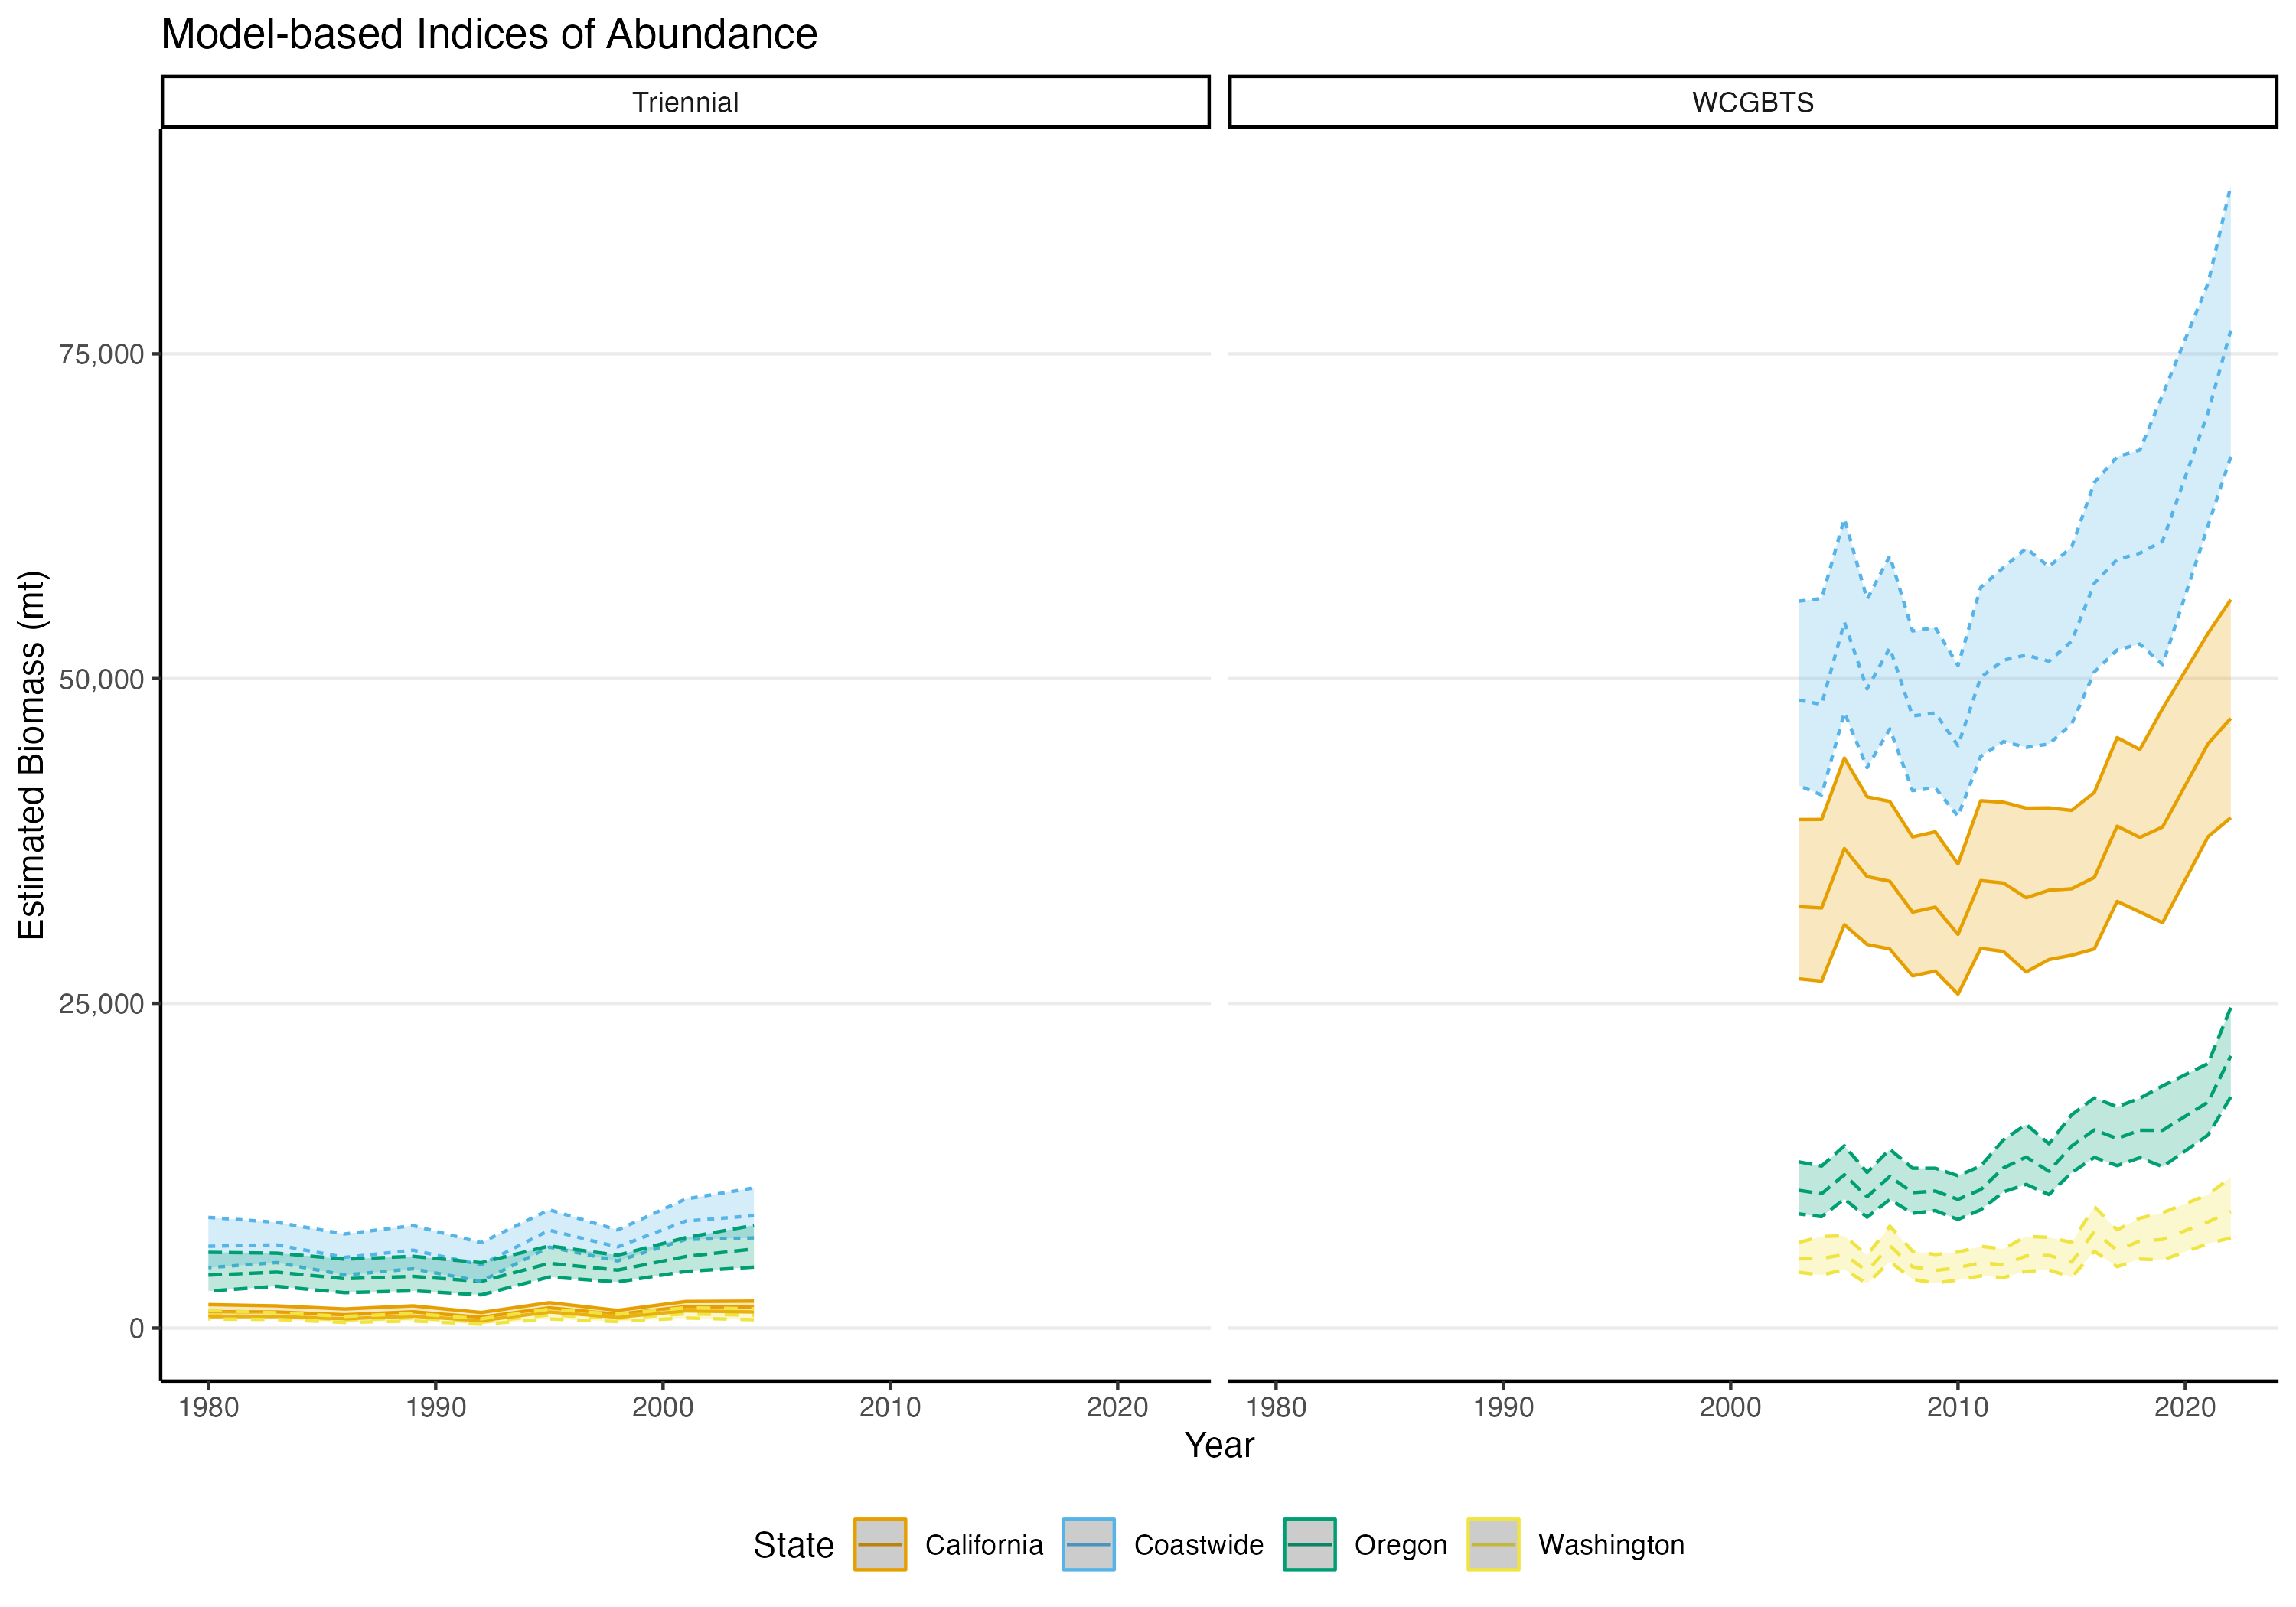
\includegraphics[width=1\textwidth,height=1\textheight]{C:/GitHub/Official_shortspine_thornyhead_2023/doc/FinalFigs/Data/geostat_indices_state_comparison.png}
\caption{State level trends in abundance indices for the Triennial Surveys and WCGBTS. Coastwide indices were computed separately and should not be interpretred as the sum of the state-level indixes.\label{fig:state_indices}}
\end{figure}

\begin{figure}
\centering
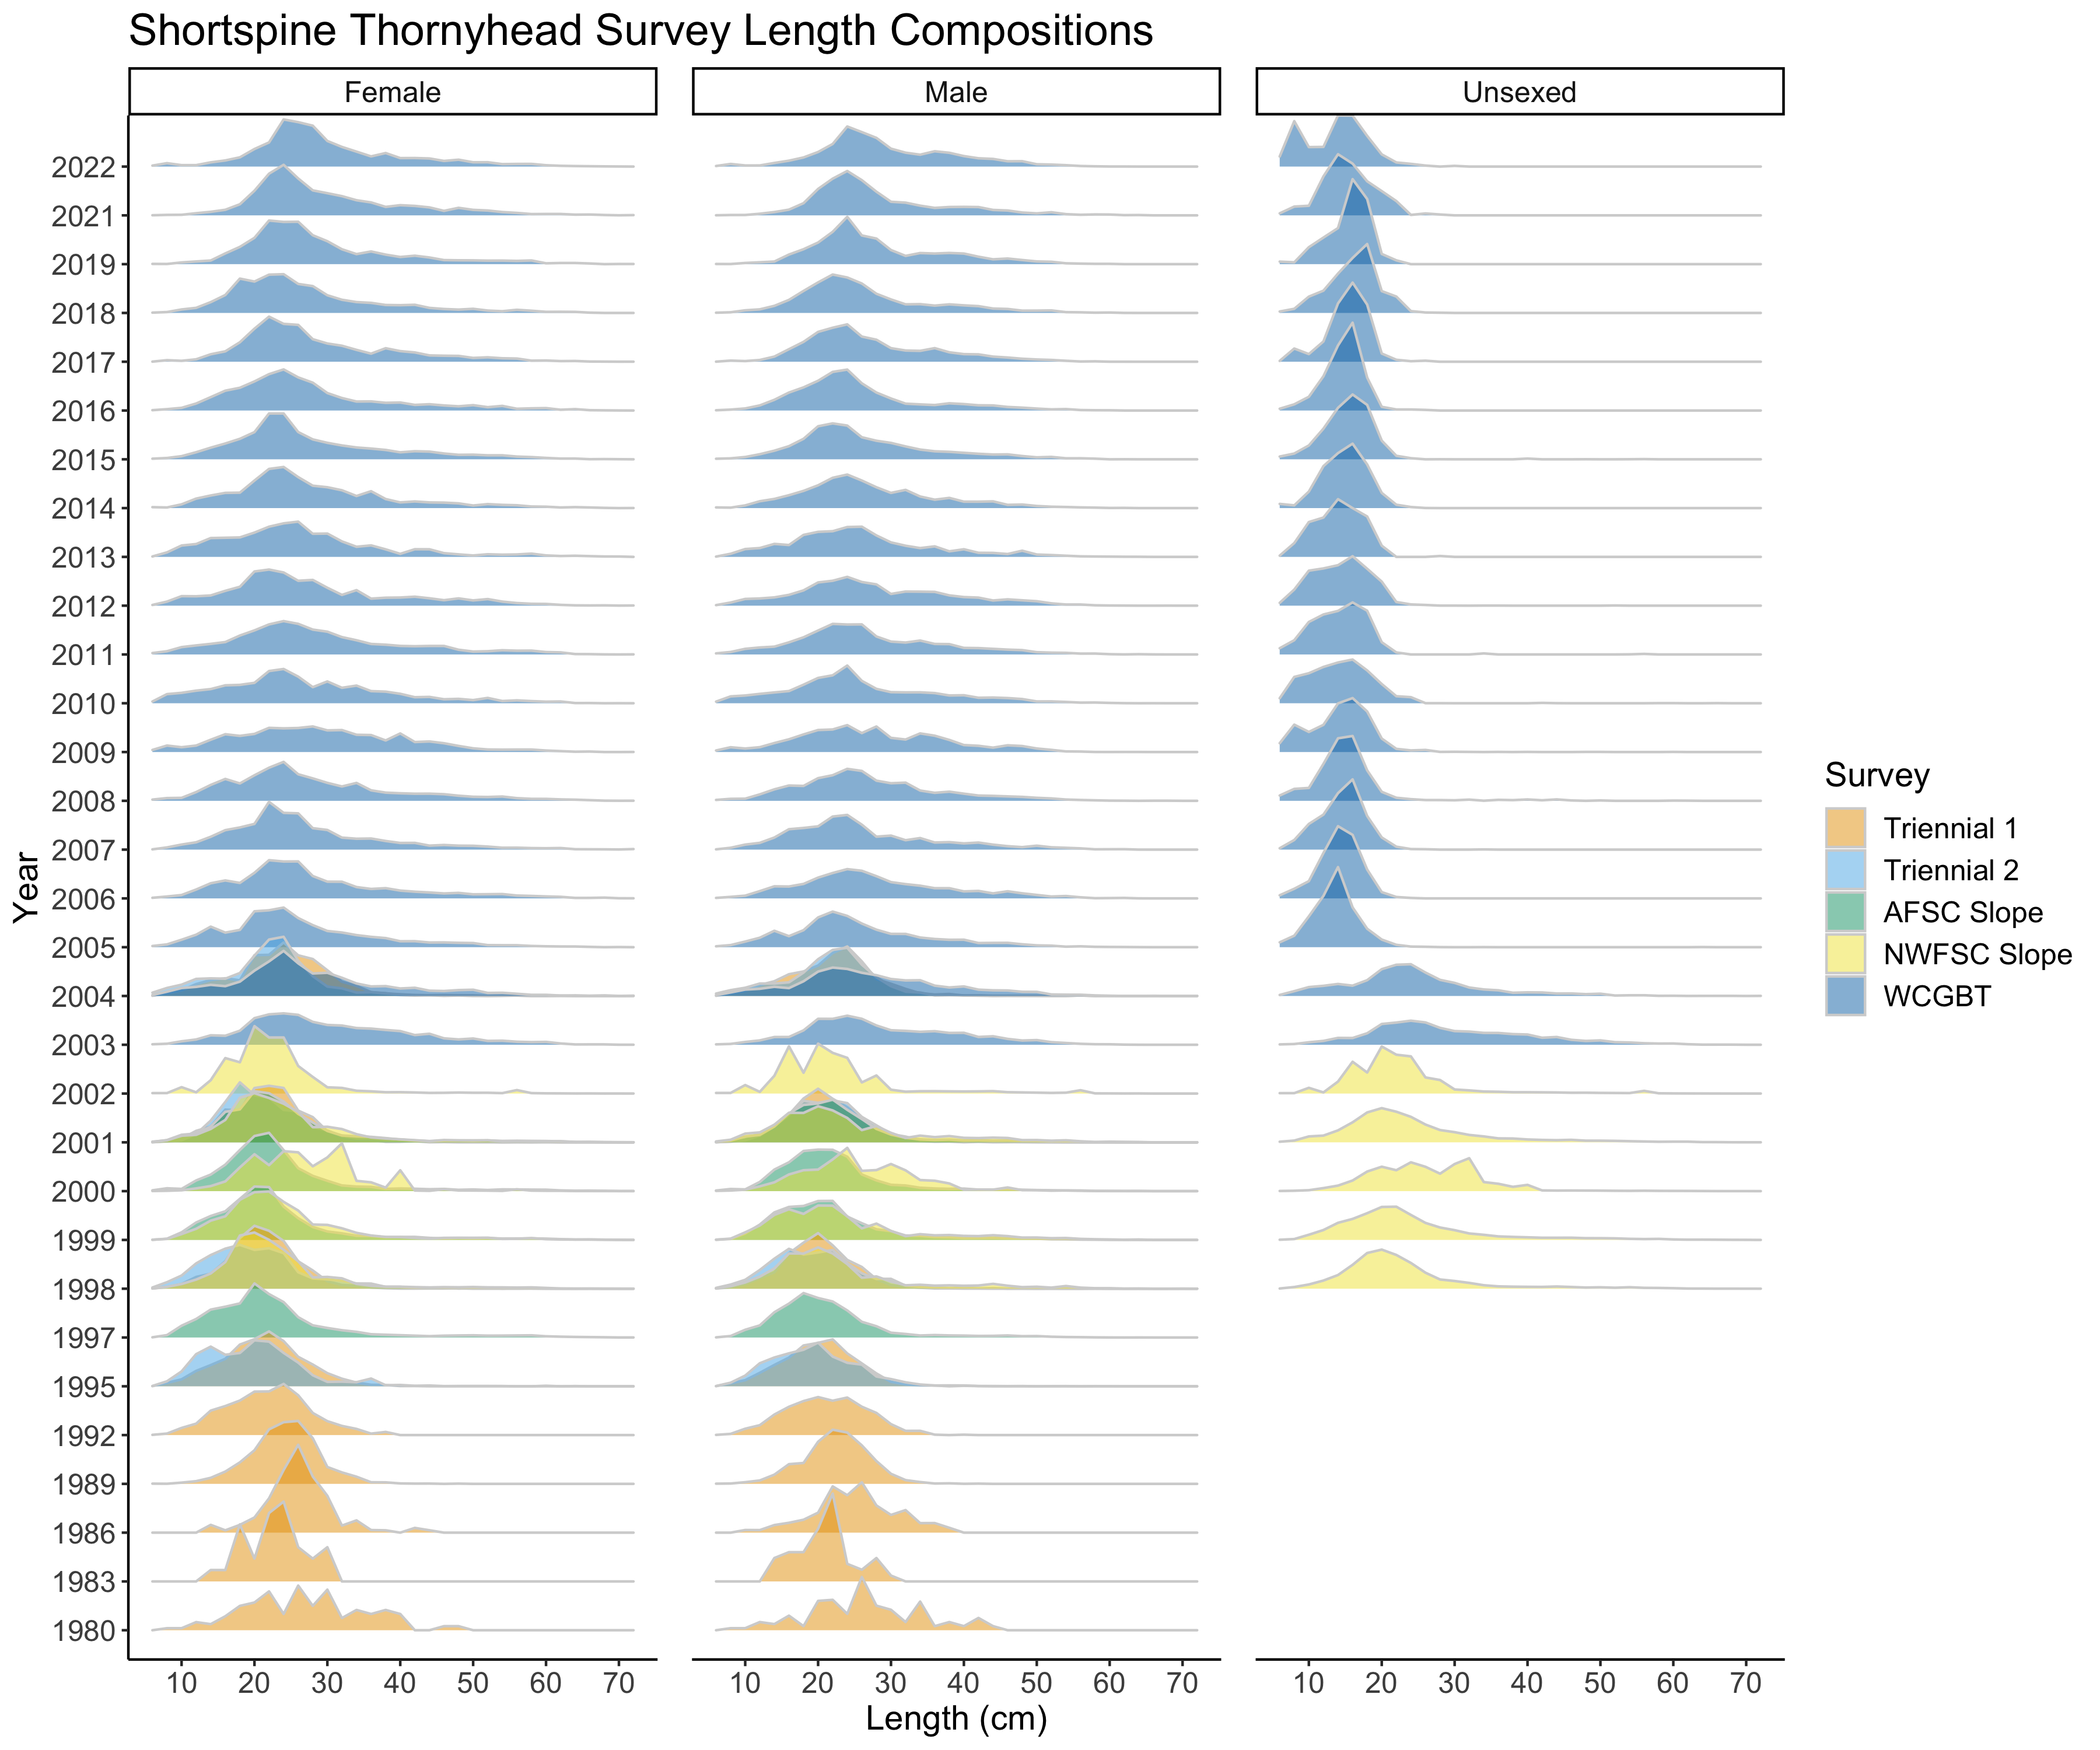
\includegraphics[width=1\textwidth,height=1\textheight]{C:/GitHub/Official_shortspine_thornyhead_2023/doc/FinalFigs/Data/2023_length_compositions.png}
\caption{Summary of annual length composition data from available scientific surveys.\label{fig:survey_comps}}
\end{figure}

\begin{figure}
\centering
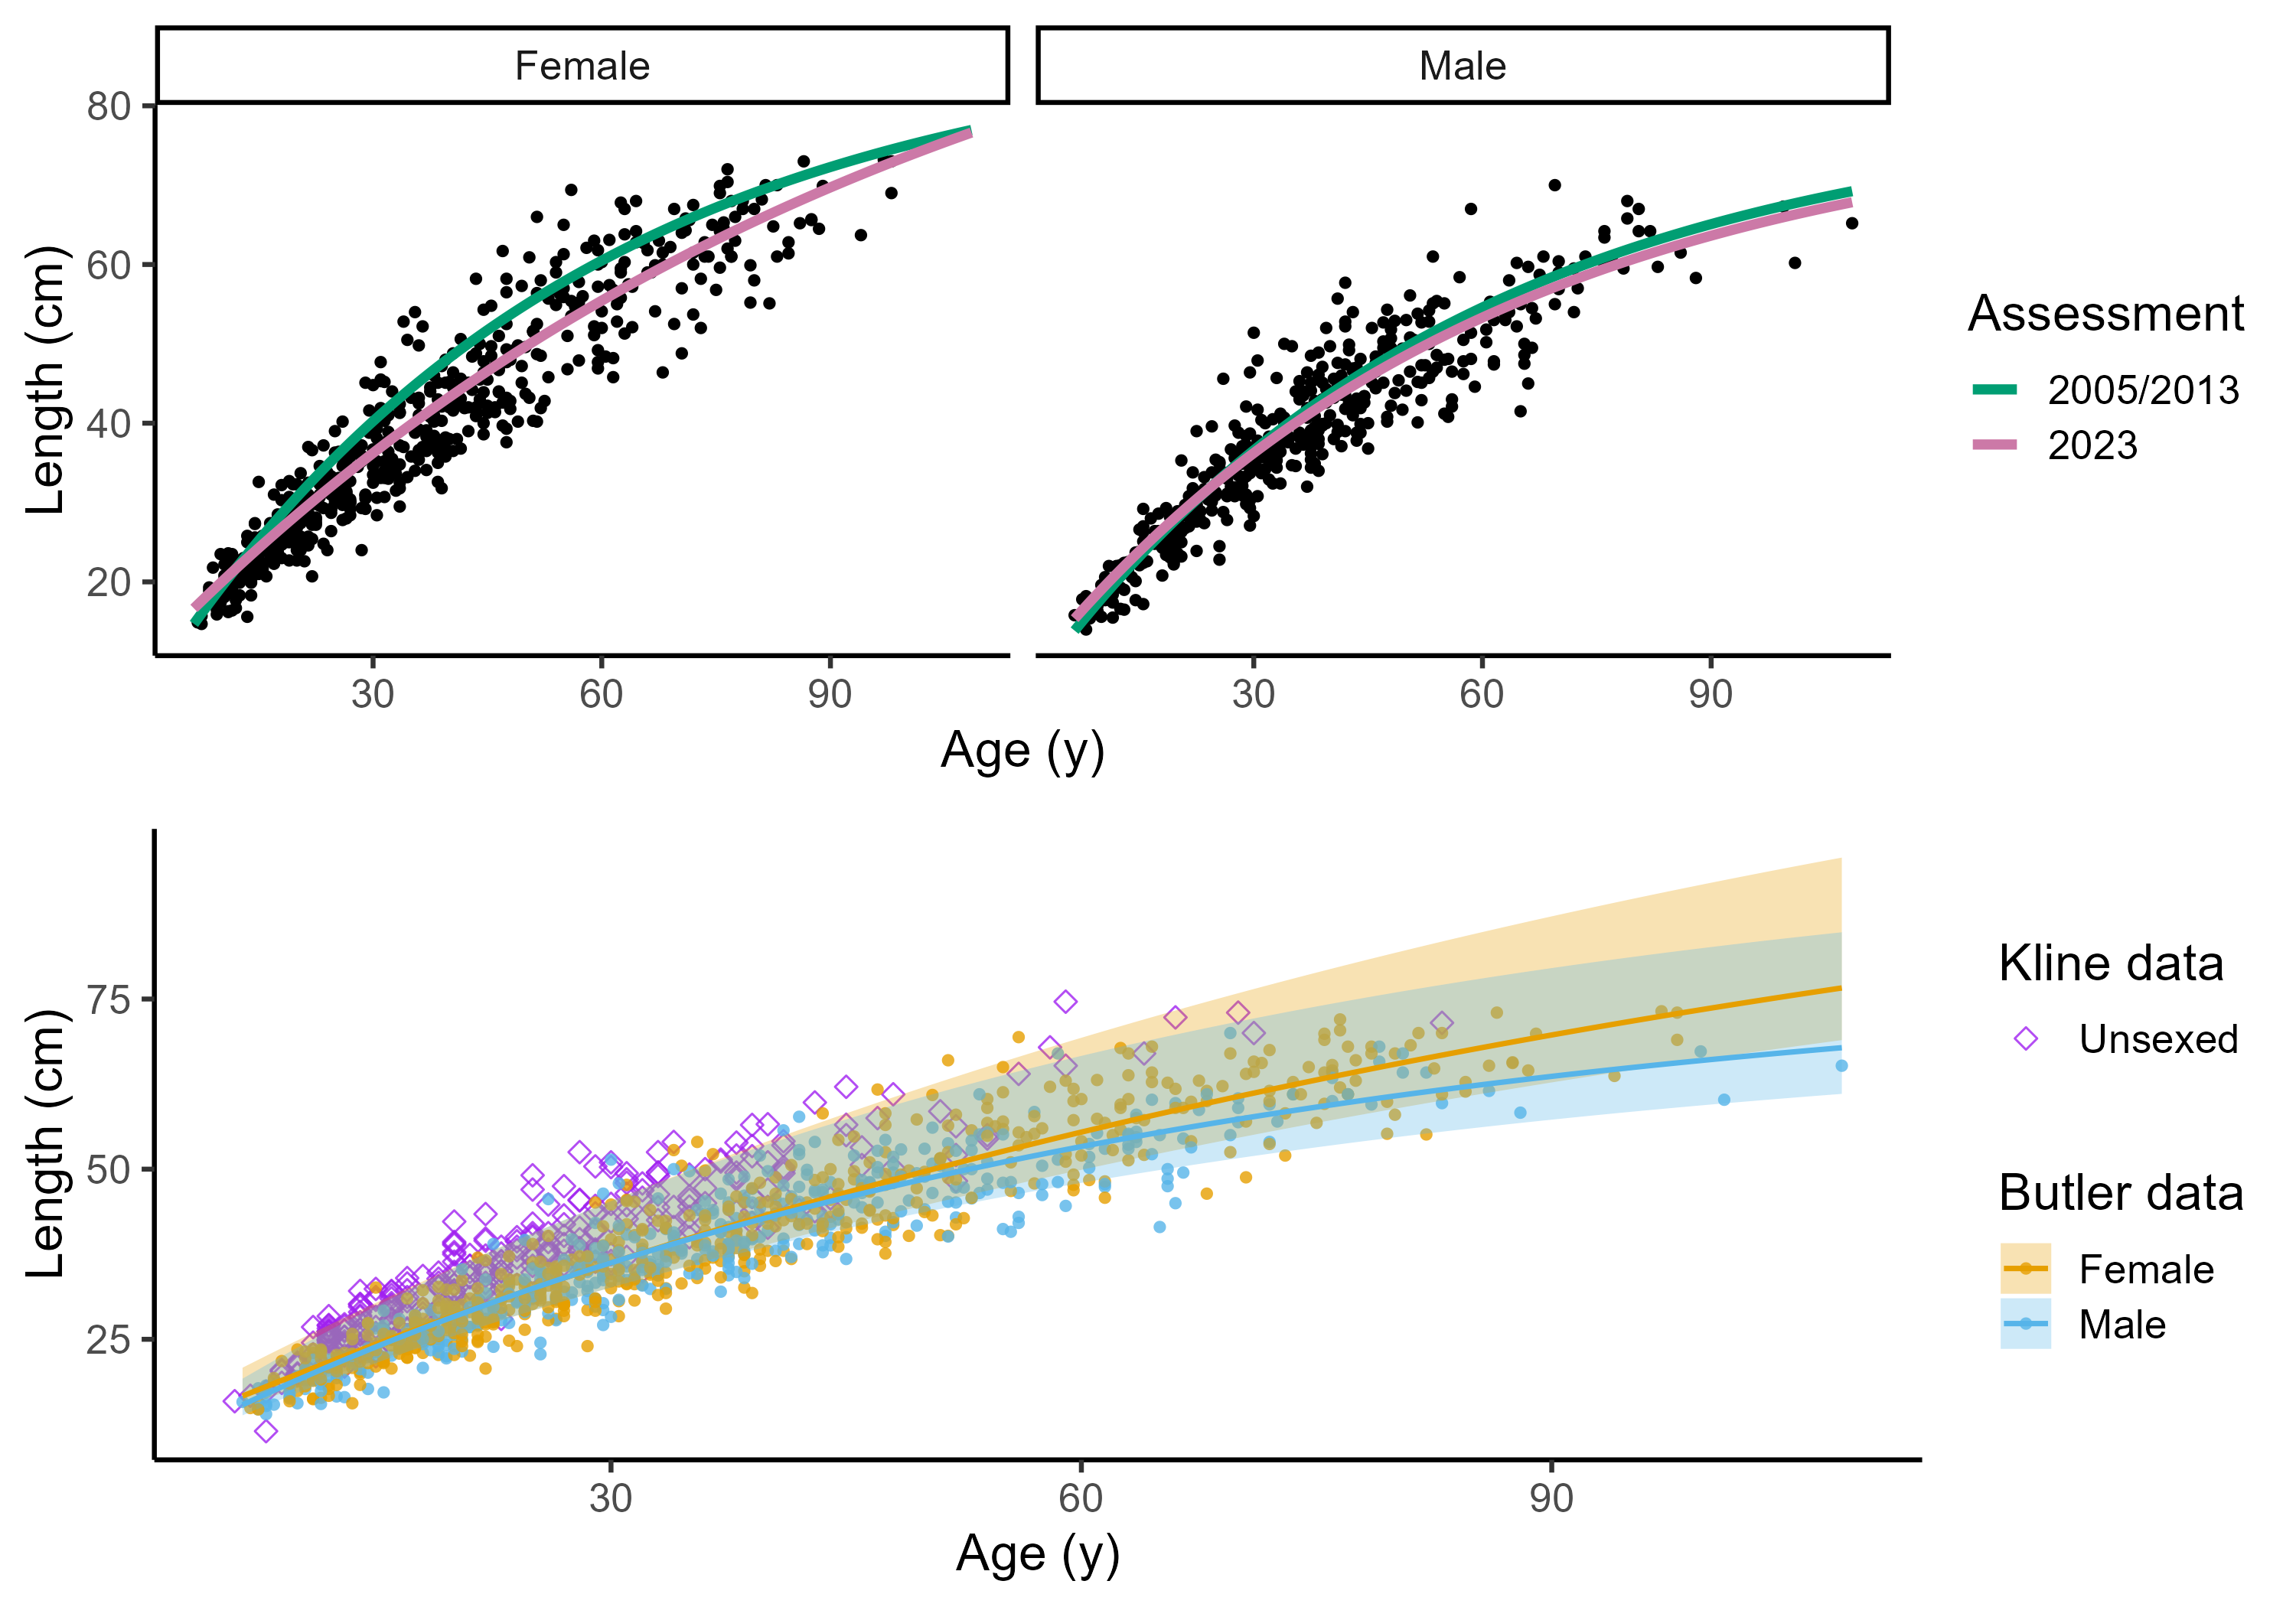
\includegraphics[width=1\textwidth,height=1\textheight]{C:/GitHub/Official_shortspine_thornyhead_2023/doc/FinalFigs/Data/growth_curves.png}
\caption{Comparison of growth curves used in the 2005/2013 assessment and the 2023 assessment, as well as high and low growth sensitivities.\label{fig:growthcurve}}
\end{figure}

\begin{figure}
\centering
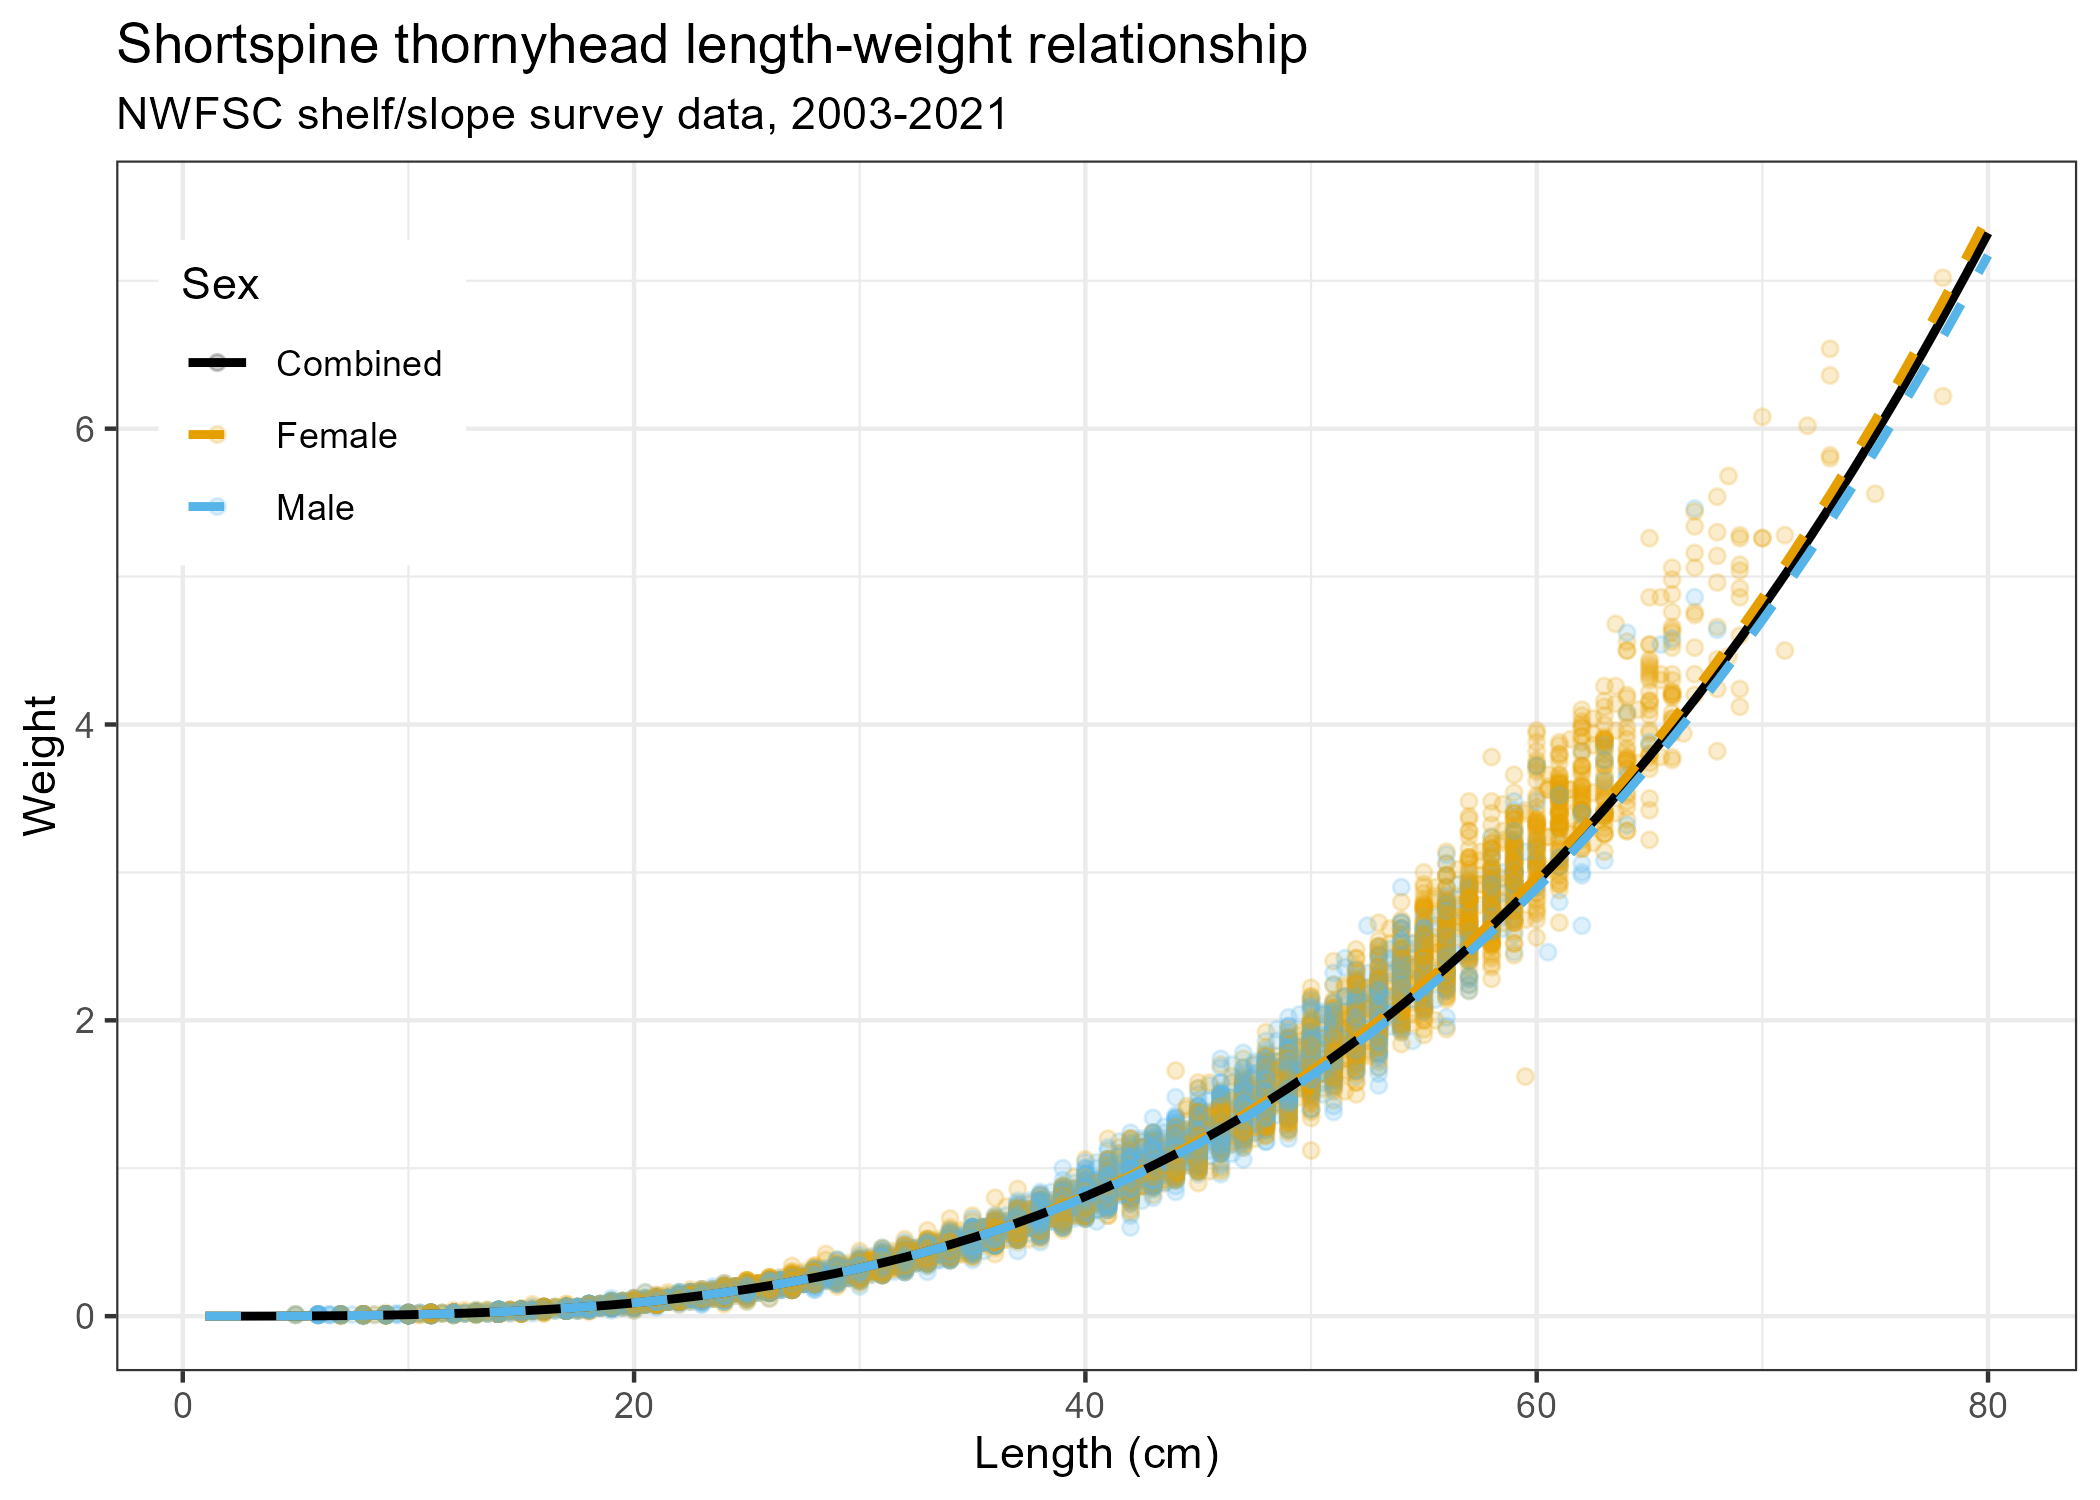
\includegraphics[width=1\textwidth,height=1\textheight]{C:/GitHub/Official_shortspine_thornyhead_2023/doc/FinalFigs/Data/lengthweight.png}
\caption{2023 length-weight relationship and fits to WCGBTS weight-length data.\label{fig:lengthweight}}
\end{figure}

\begin{figure}
\centering
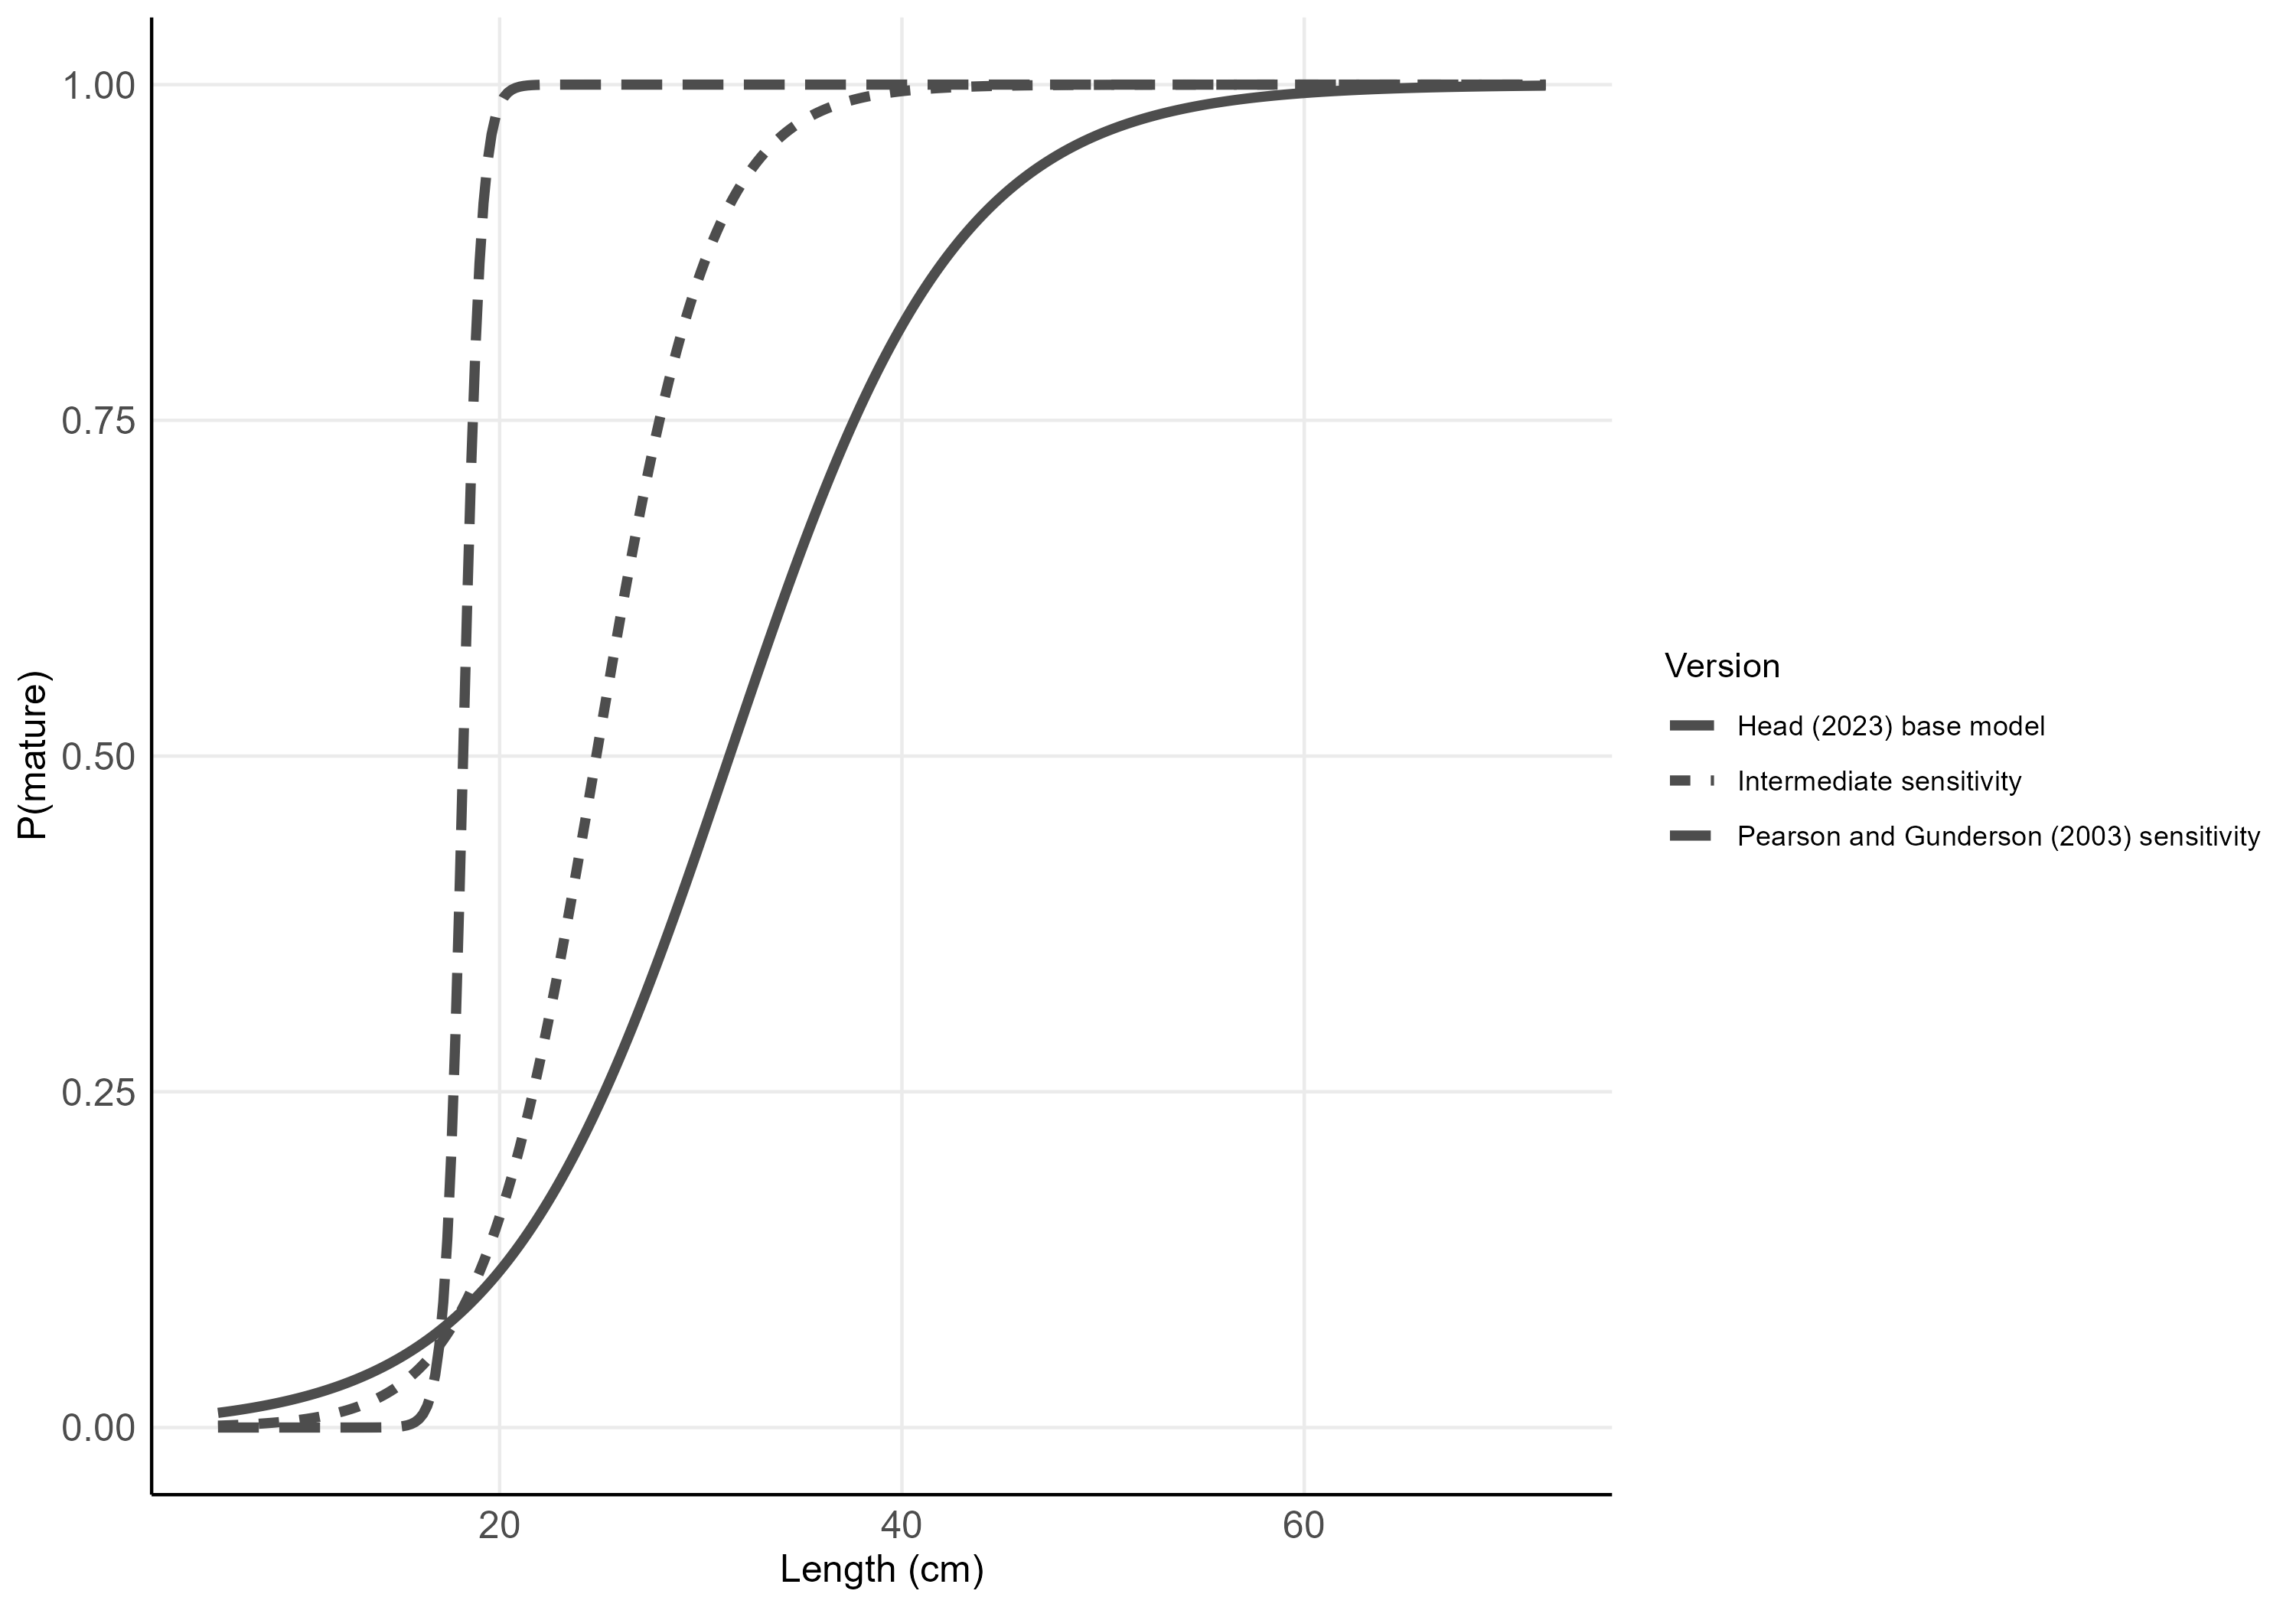
\includegraphics[width=1\textwidth,height=1\textheight]{C:/GitHub/Official_shortspine_thornyhead_2023/doc/FinalFigs/Data/comparison_alternative_maturity_curves.png}
\caption{Maturity curves considered in the present assessment (Head (2023)) and alternative versions considered in the sensitivity analysis.\label{fig:mat2}}
\end{figure}

\begin{figure}
\centering
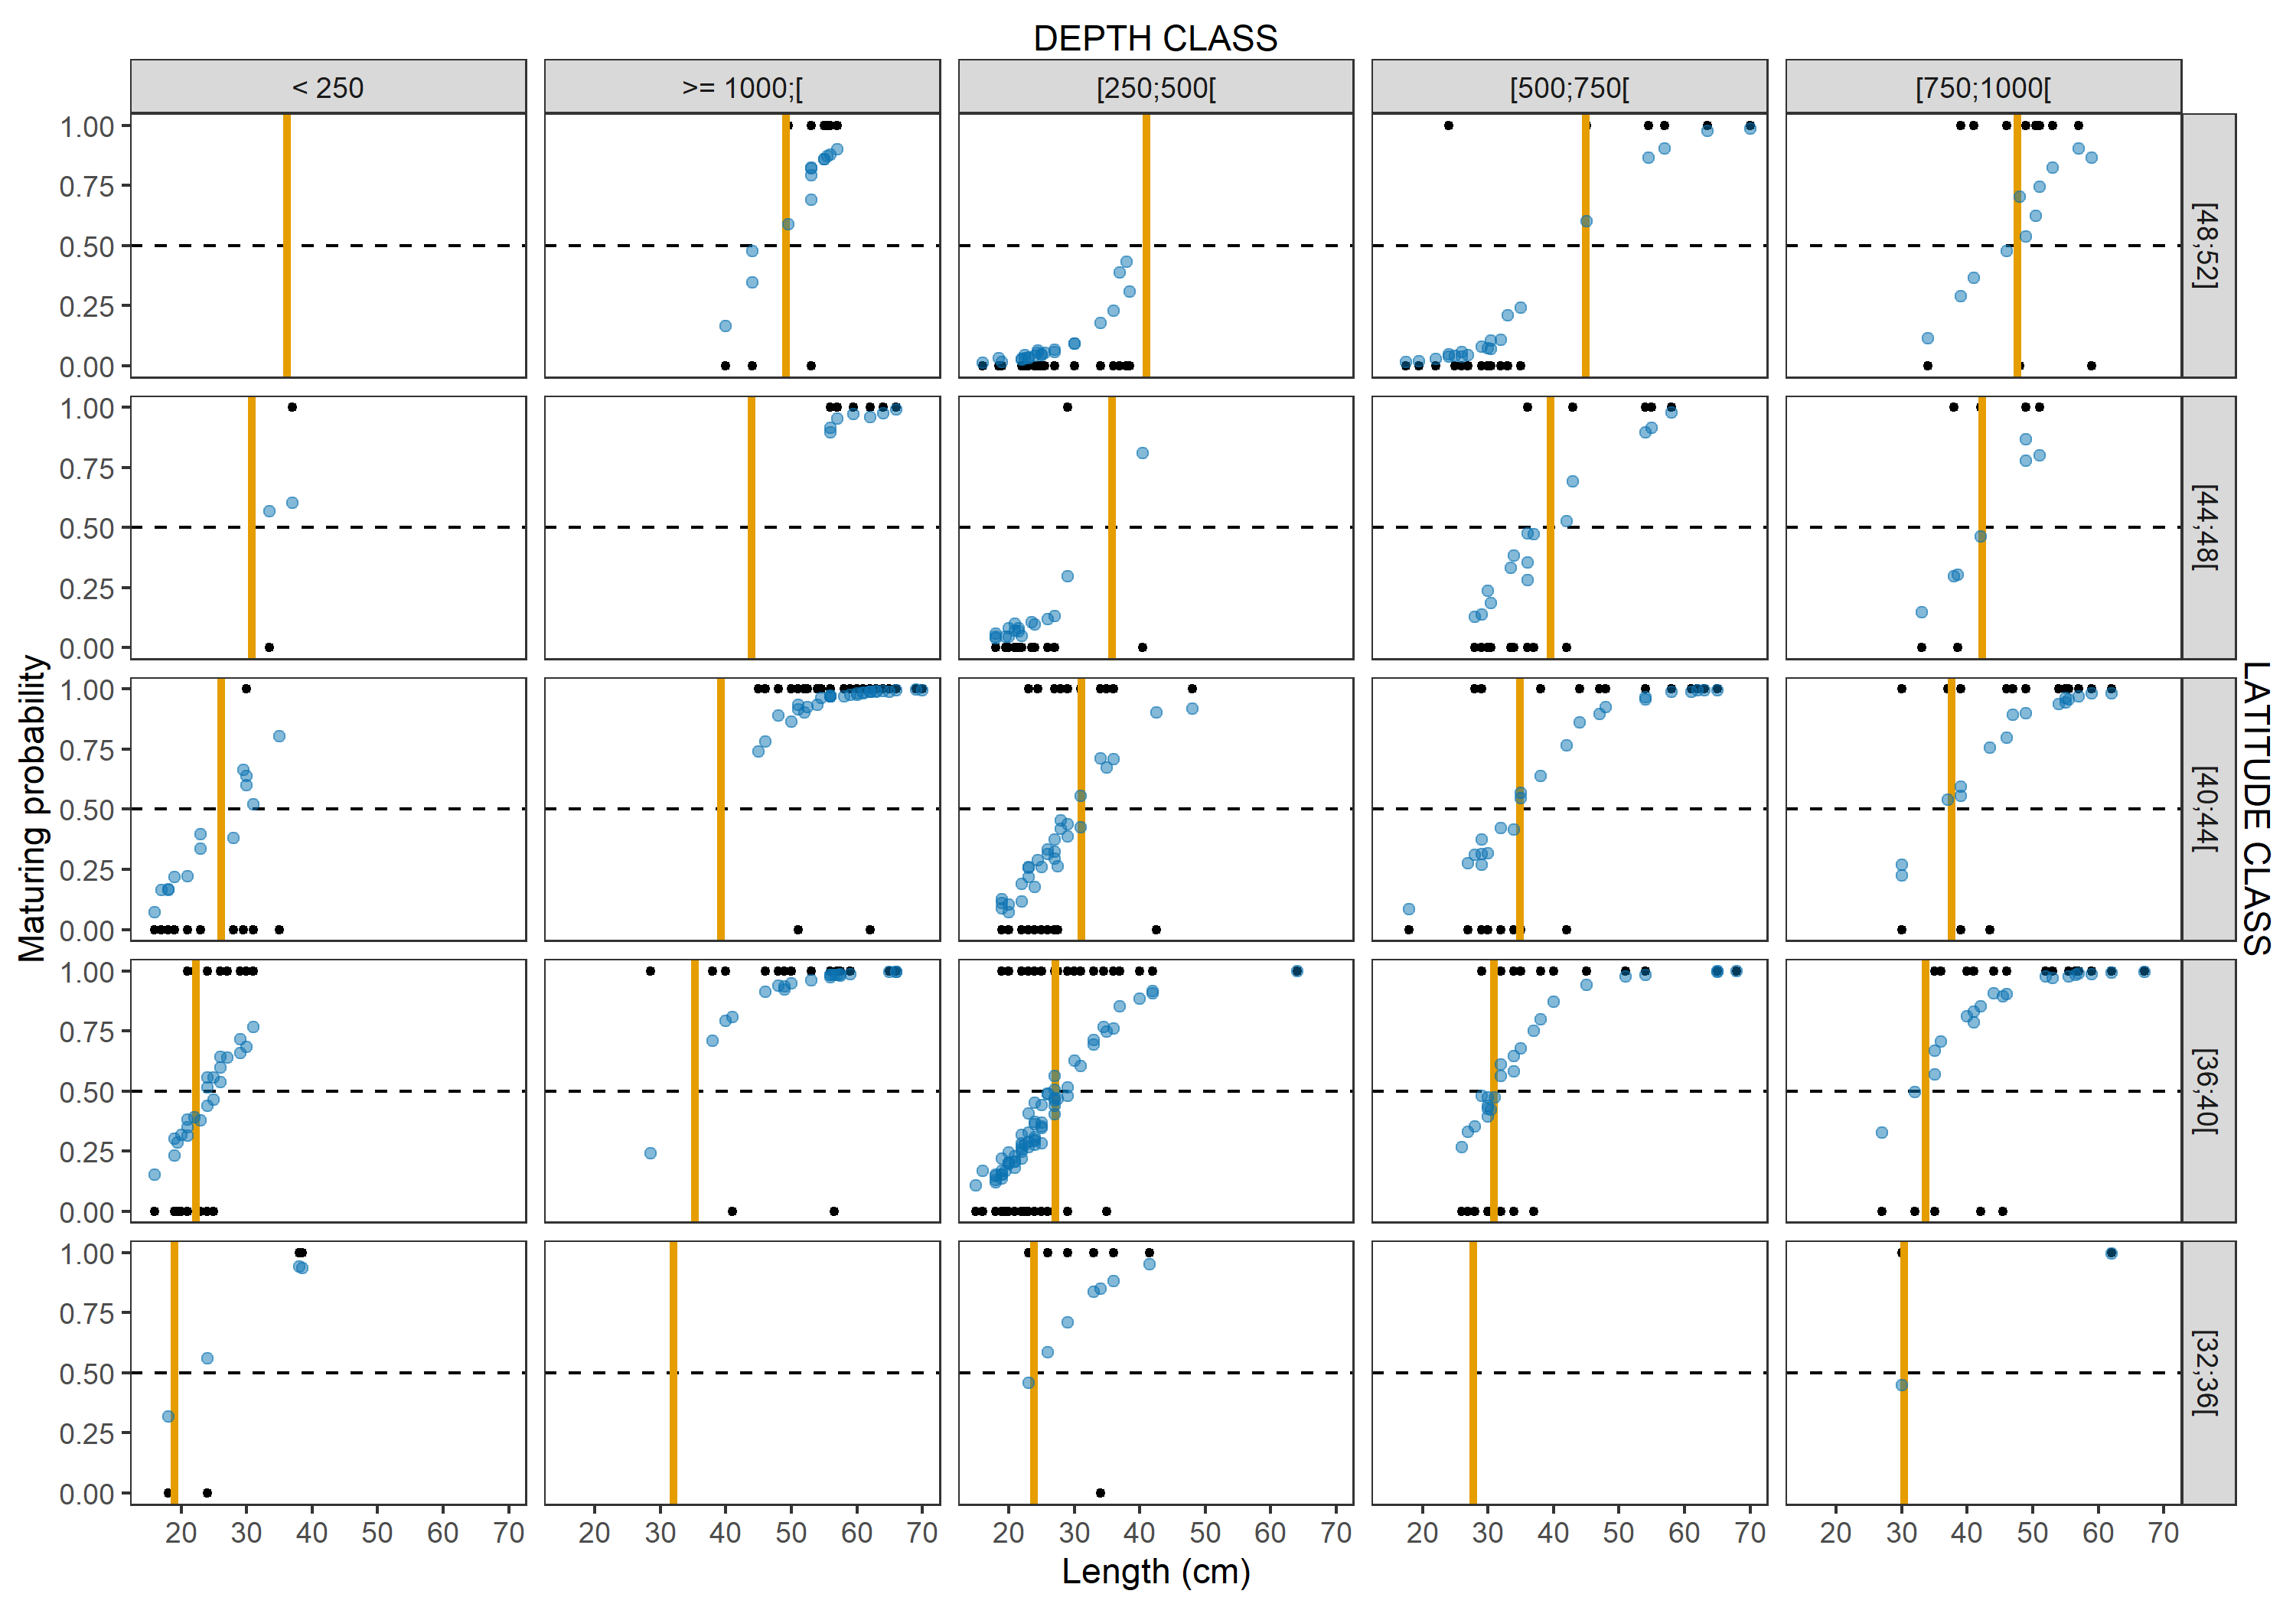
\includegraphics[width=1\textwidth,height=1\textheight]{C:/GitHub/Official_shortspine_thornyhead_2023/doc/FinalFigs/Data/head2023_maturity_latdepth_glm_fit.png}
\caption{Fit of the maturity curves per size and depth classes. Classes are designed for visual check of the model predictions only since the model assumes continuous and not categorical response to these variables.\label{fig:mat1}}
\end{figure}

\begin{figure}
\centering
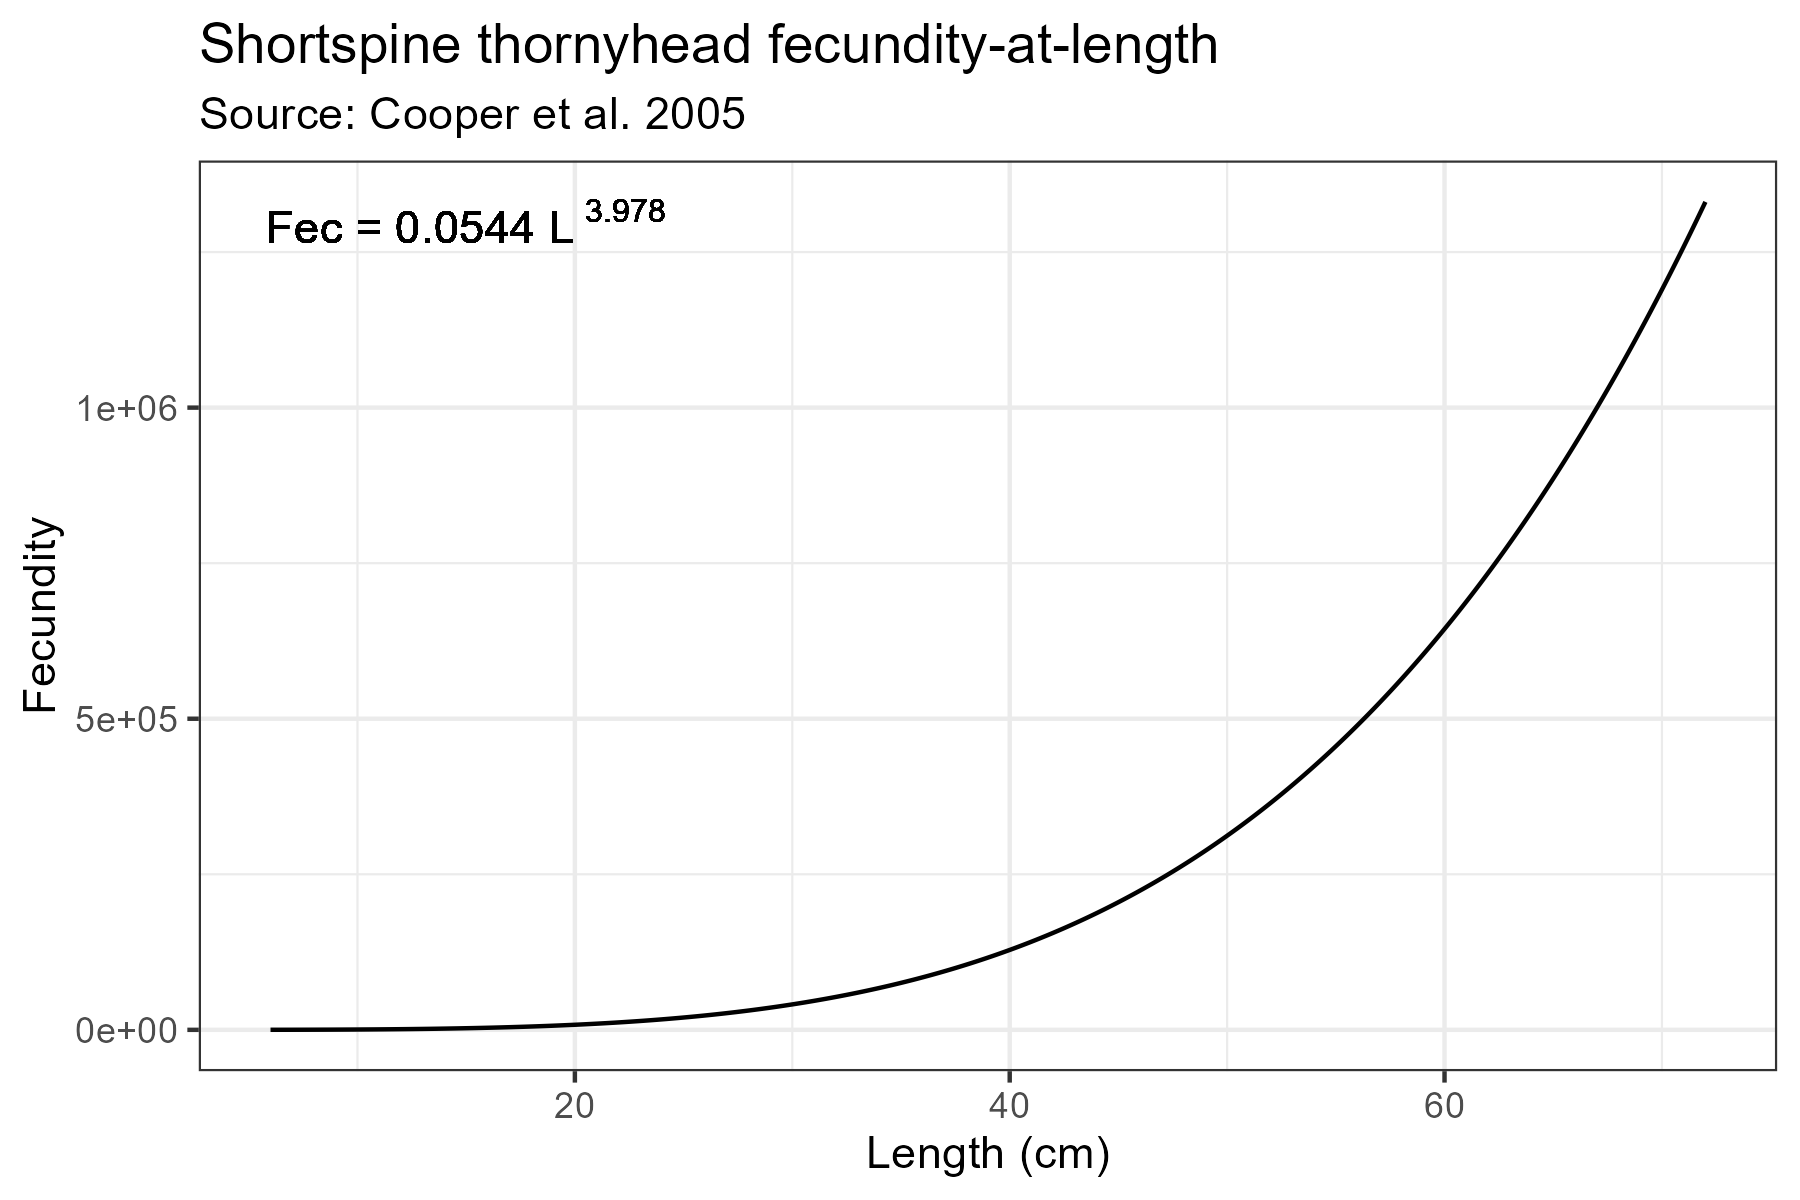
\includegraphics[width=1\textwidth,height=1\textheight]{C:/GitHub/Official_shortspine_thornyhead_2023/doc/FinalFigs/Data/fecundity.png}
\caption{Fecundity-at-length relationship.\label{fig:fec}}
\end{figure}

\clearpage

\hypertarget{bridging-analyses}{%
\subsection{Bridging Analyses}\label{bridging-analyses}}

\begin{figure}
\centering
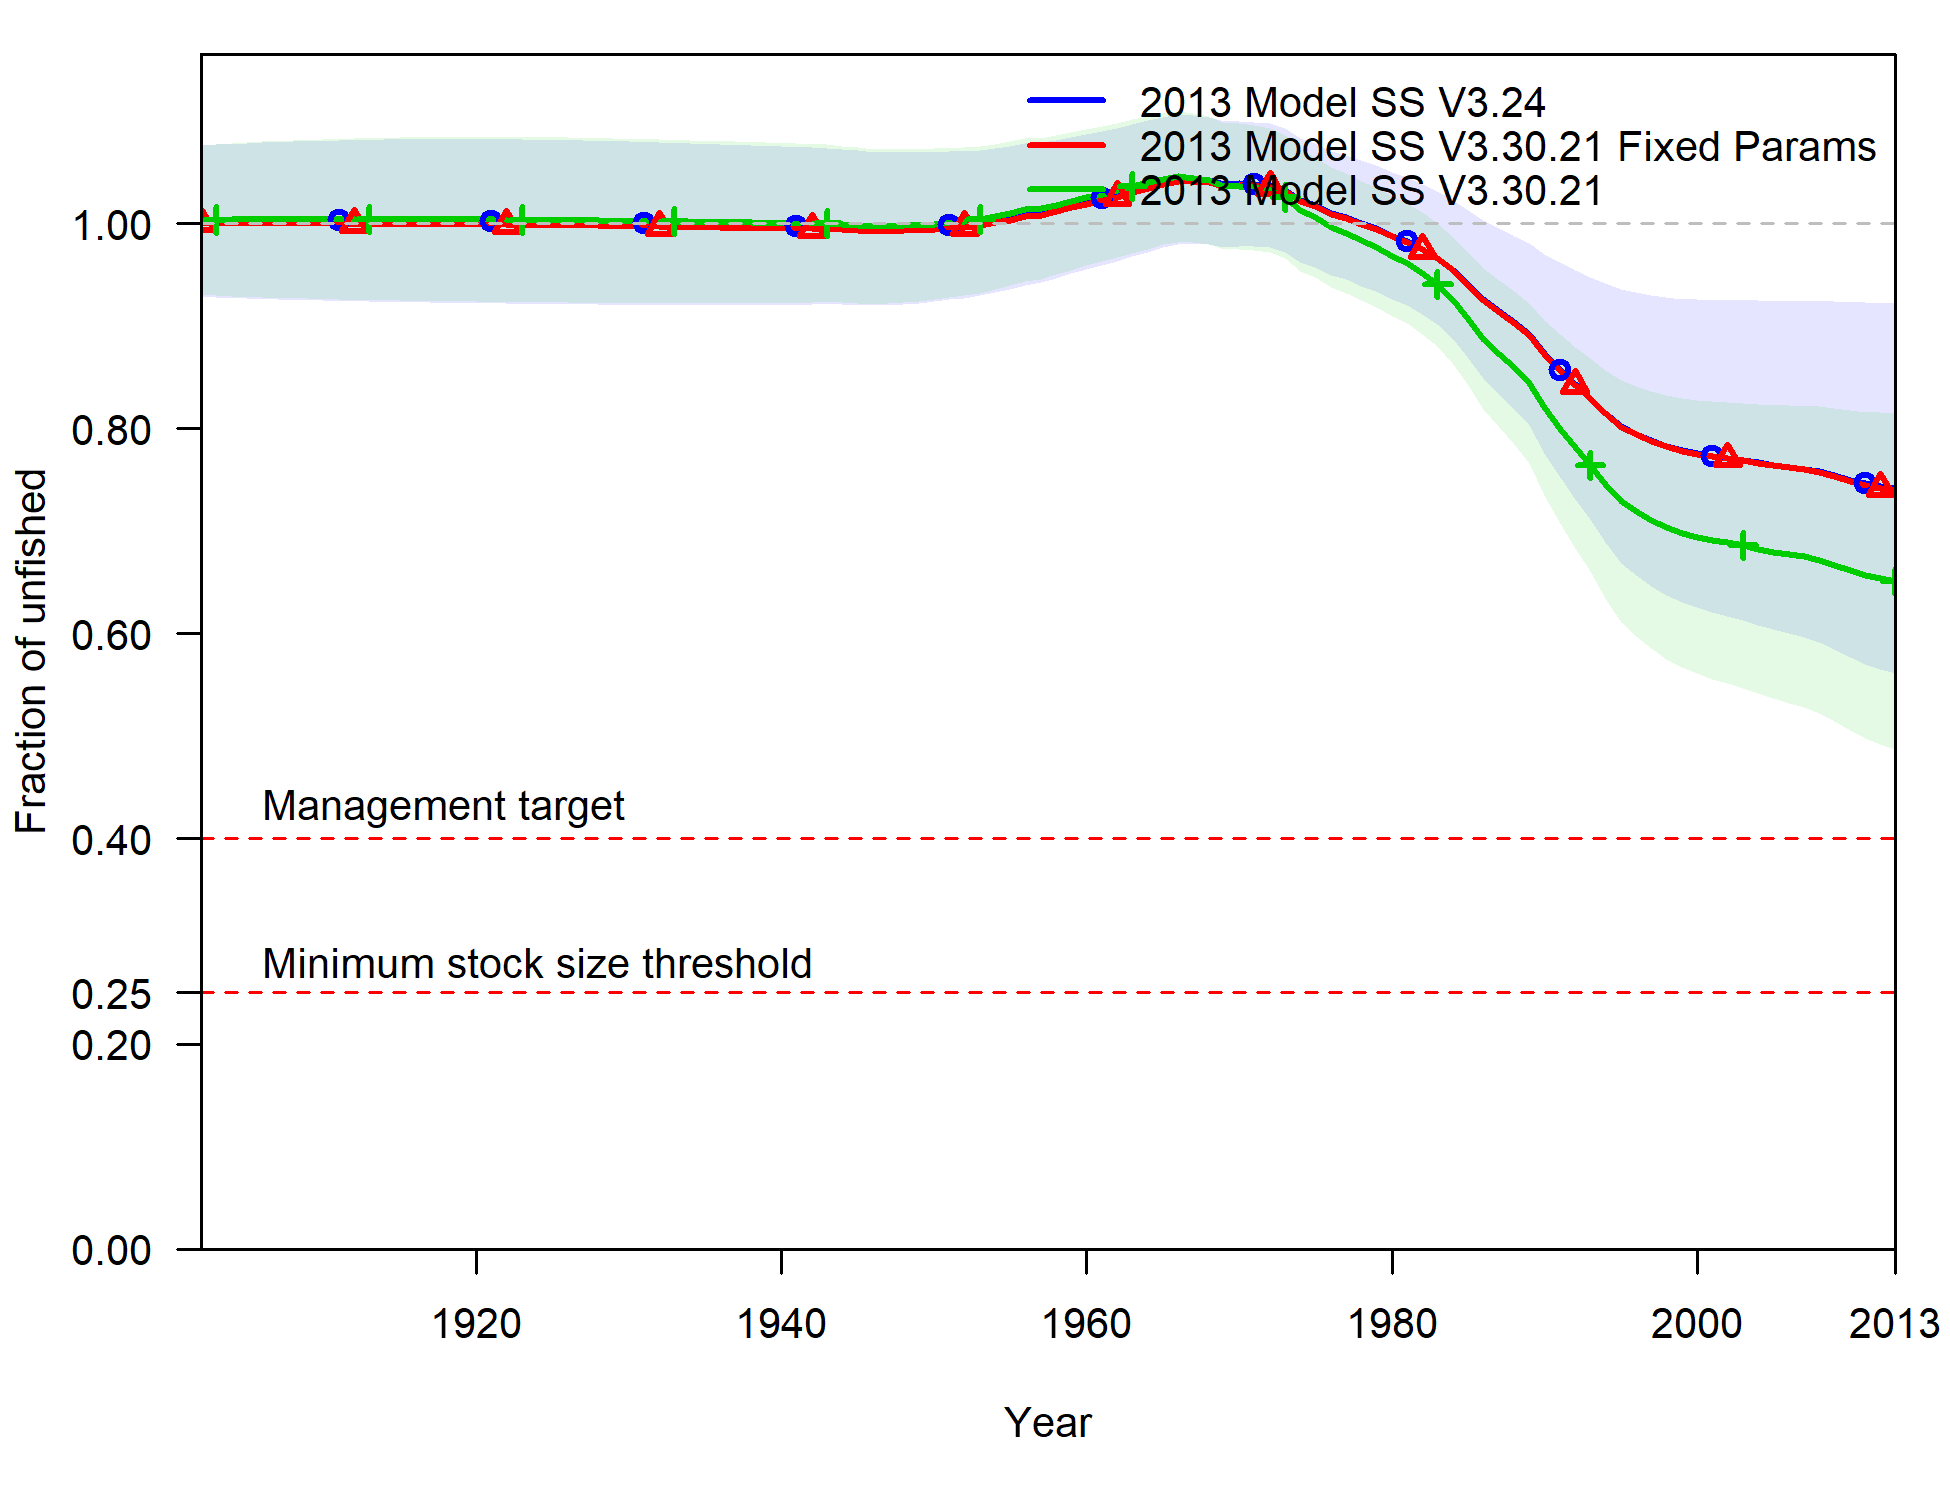
\includegraphics[width=1\textwidth,height=1\textheight]{C:/GitHub/Official_shortspine_thornyhead_2023/doc/FinalFigs/bridging/Bridg_ts2_Bratio.png}
\caption{Relative spawning biomass timeseries for models run on updated Stock Synthesis versions.\label{fig:bridge_bratio}}
\end{figure}

\begin{figure}
\centering
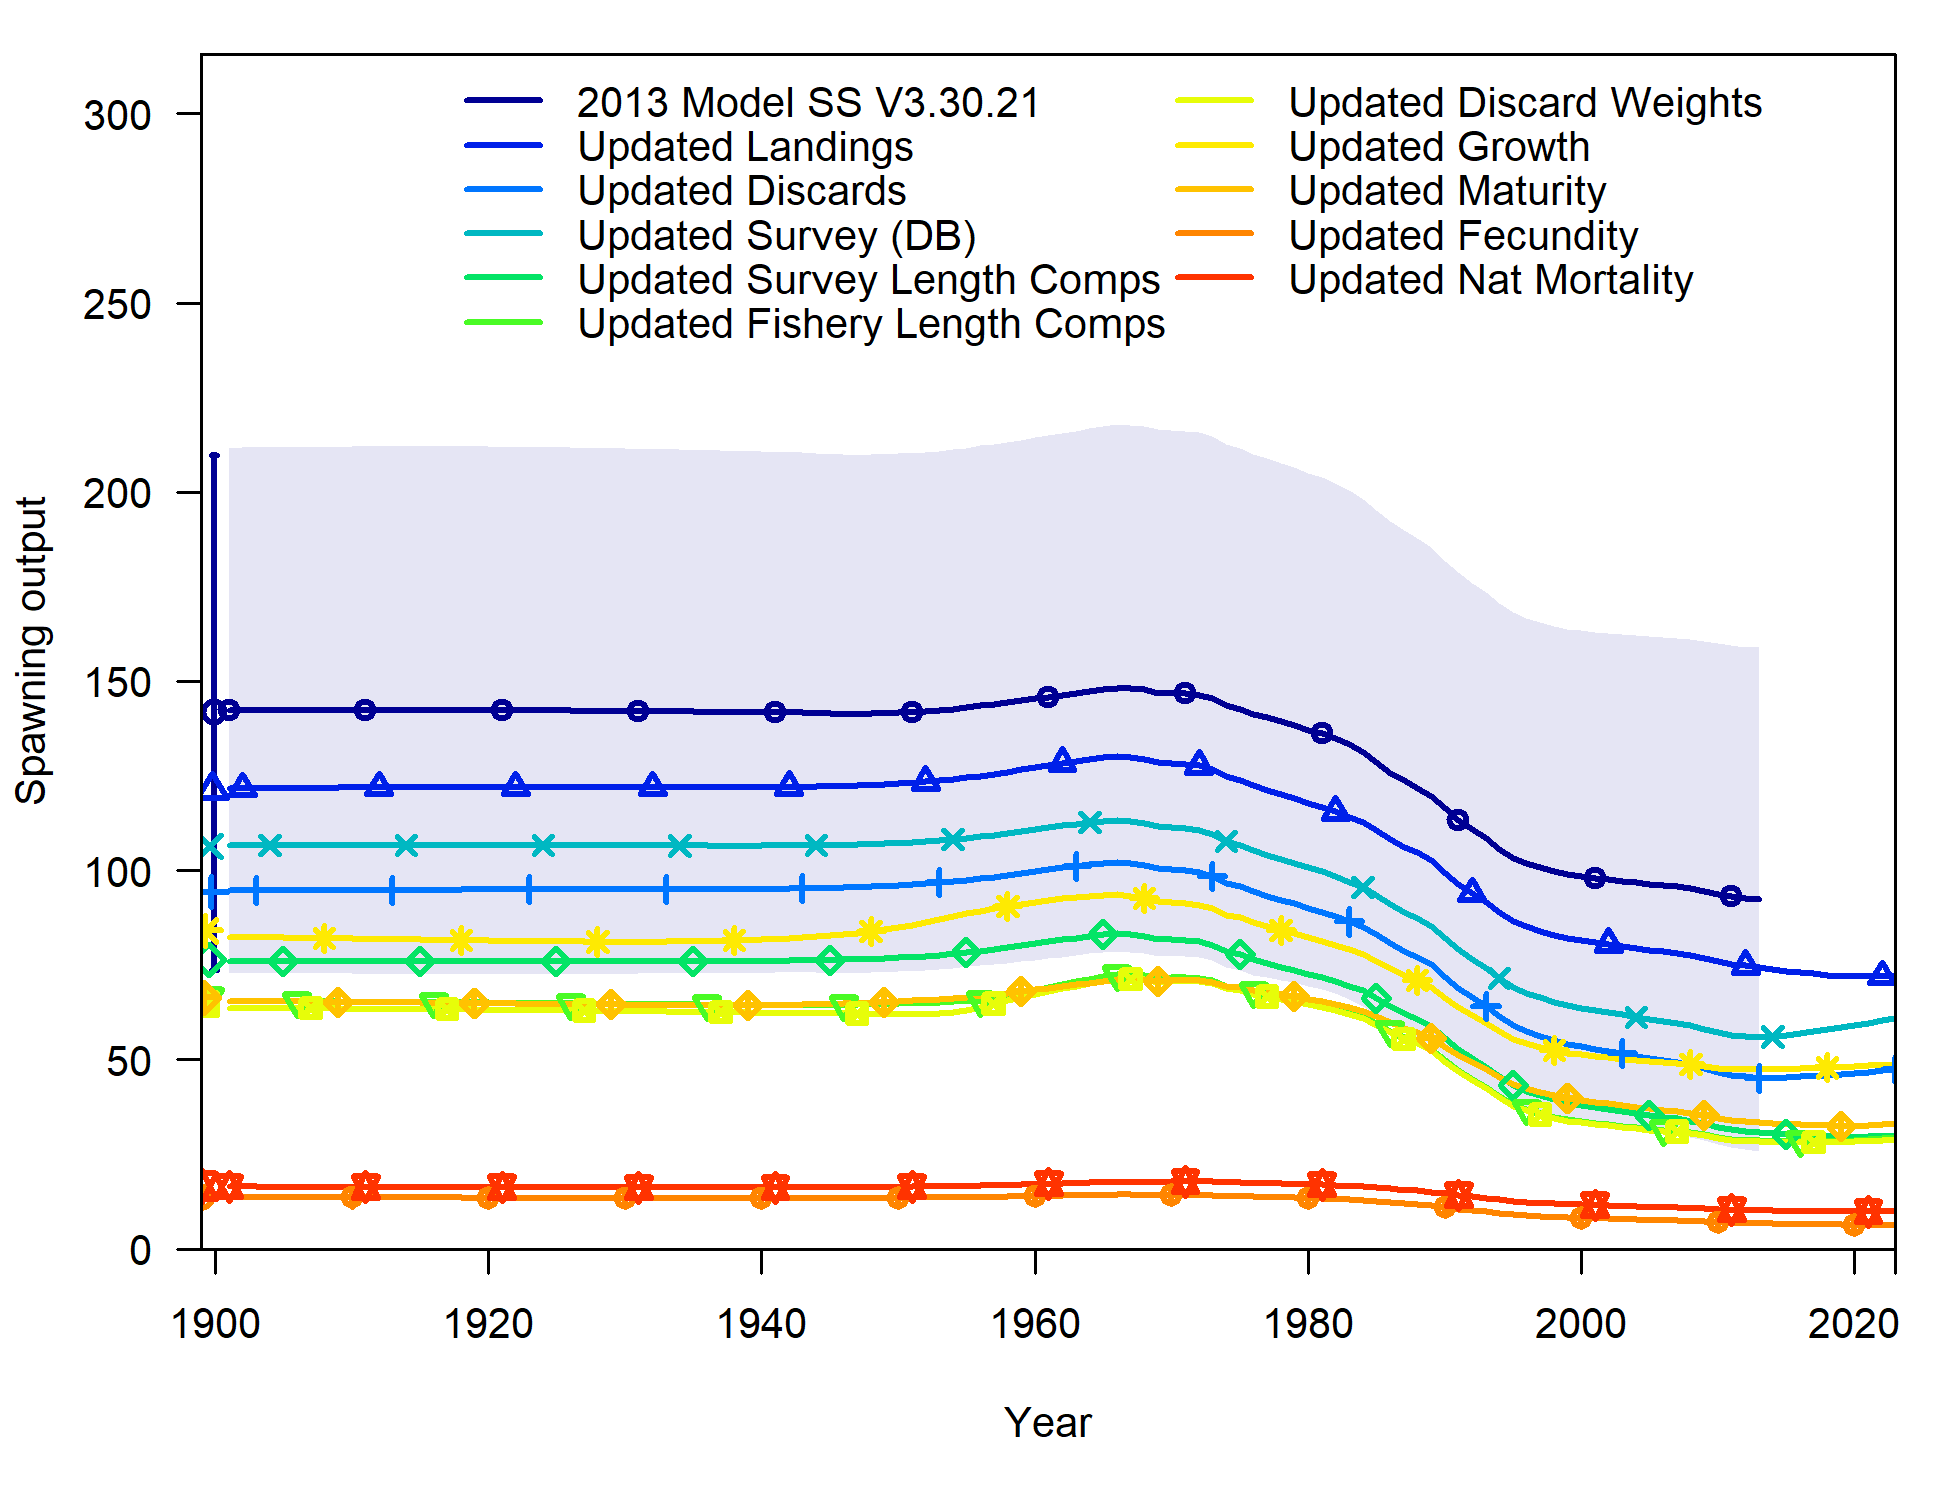
\includegraphics[width=1\textwidth,height=1\textheight]{C:/GitHub/Official_shortspine_thornyhead_2023/doc/FinalFigs/bridging/Bridg_ts3_Spawning_Output.png}
\caption{Spawning output timeseries for piecewise data updates.\label{fig:bridge_spawnout_data}}
\end{figure}

\begin{figure}
\centering
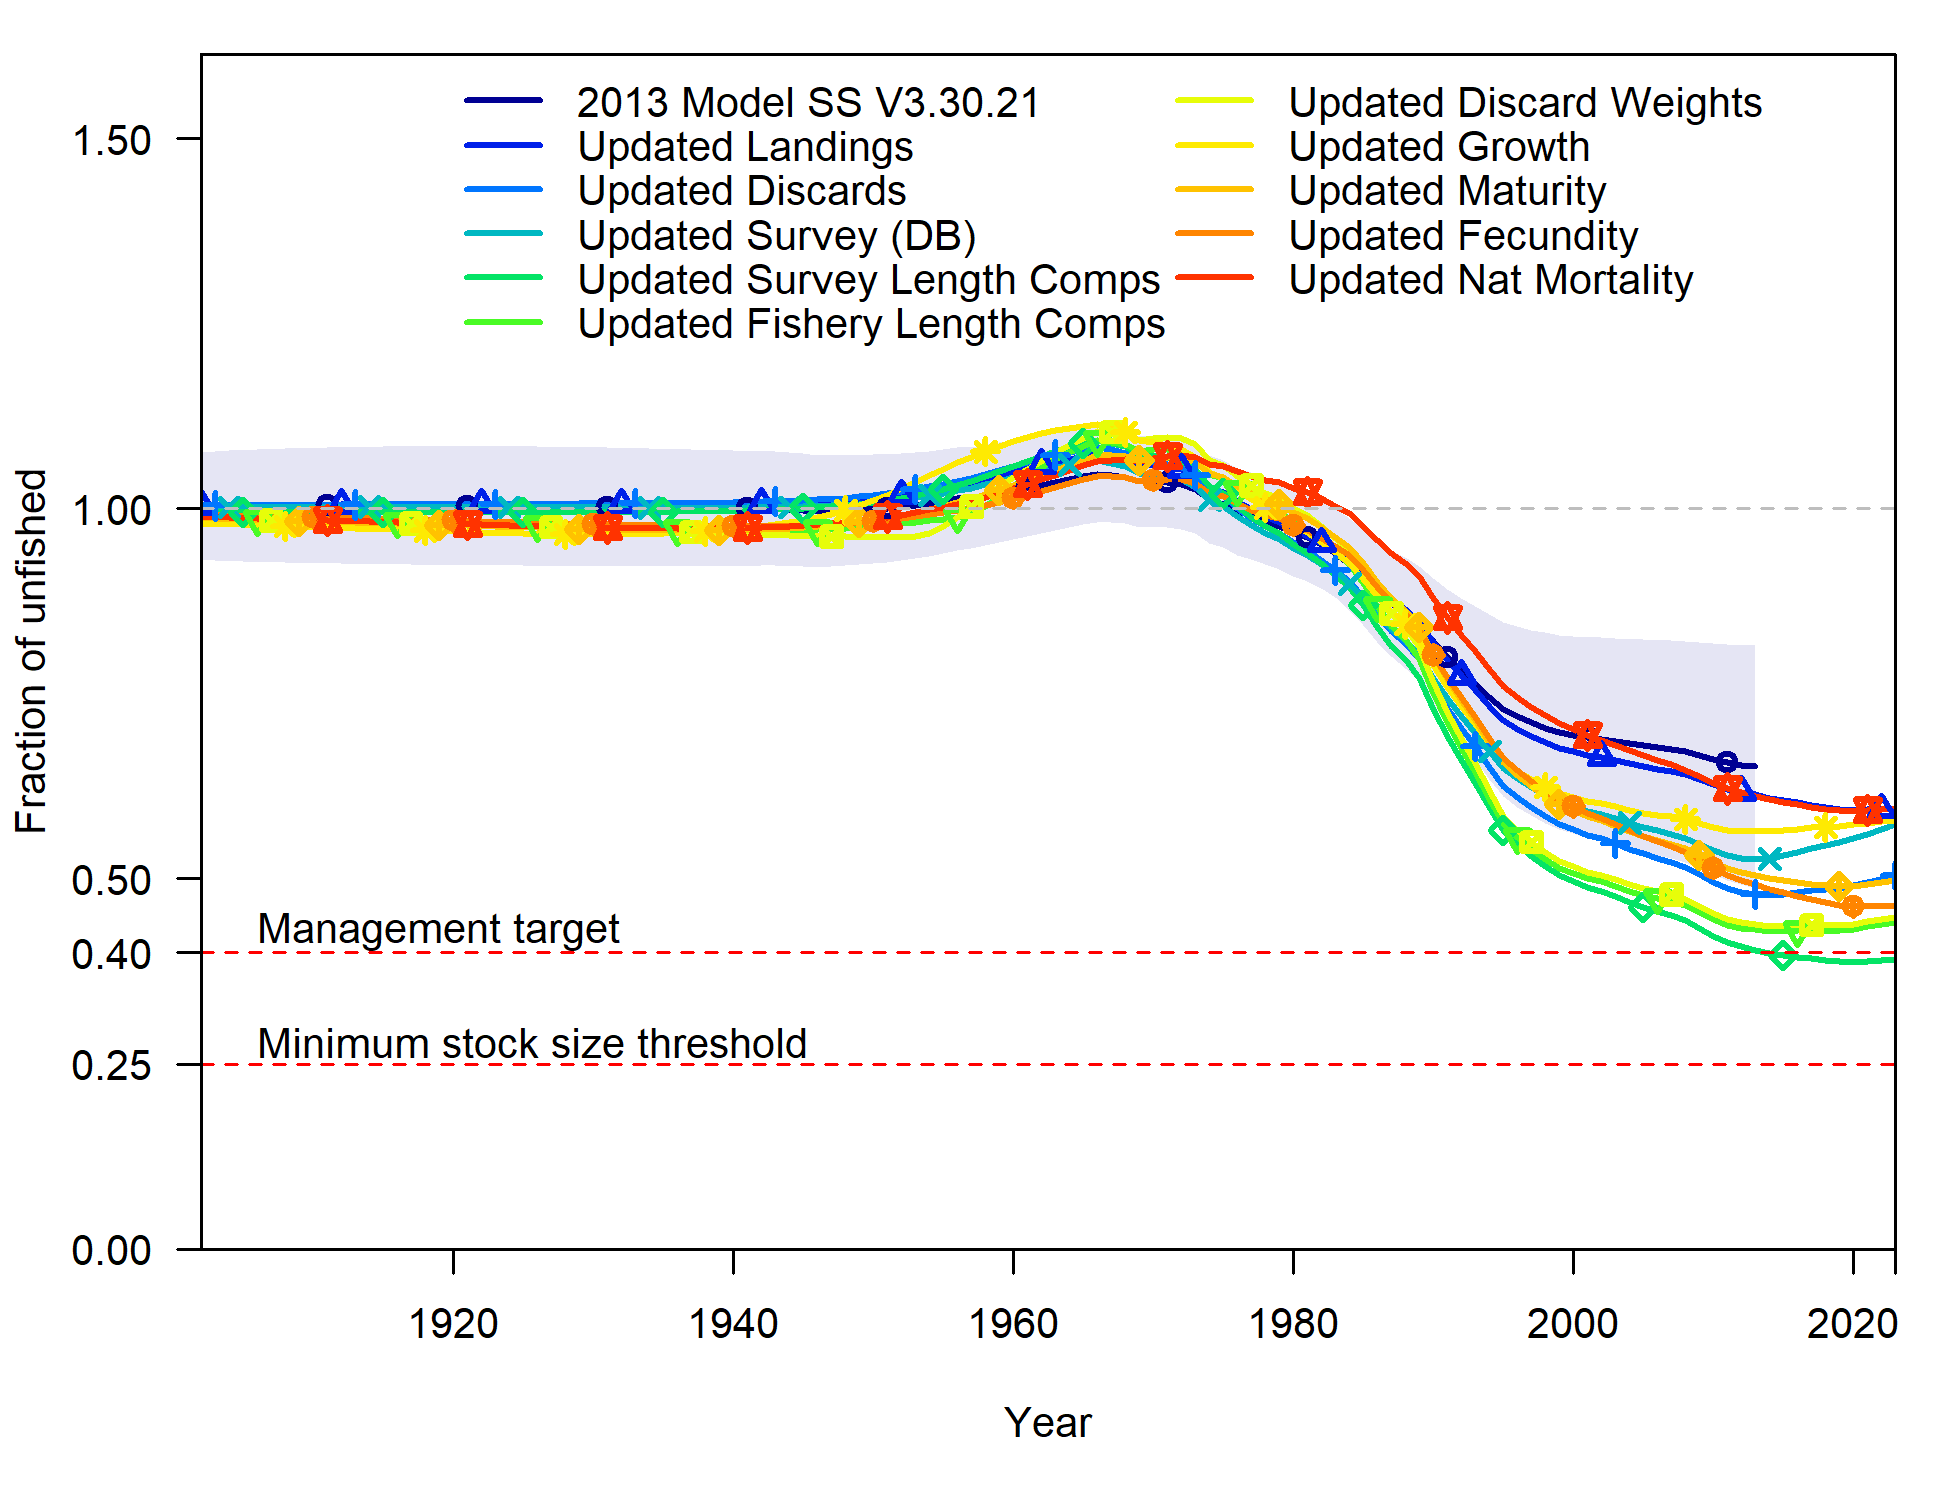
\includegraphics[width=1\textwidth,height=1\textheight]{C:/GitHub/Official_shortspine_thornyhead_2023/doc/FinalFigs/bridging/Bridg_ts4_Bratio.png}
\caption{Relative spawning biomass timeseries for piecewise data updates.\label{fig:bridge_bratio_data}}
\end{figure}

\clearpage

\hypertarget{base-model-results-and-fits}{%
\subsection{Base Model Results and Fits}\label{base-model-results-and-fits}}

\begin{figure}
\centering
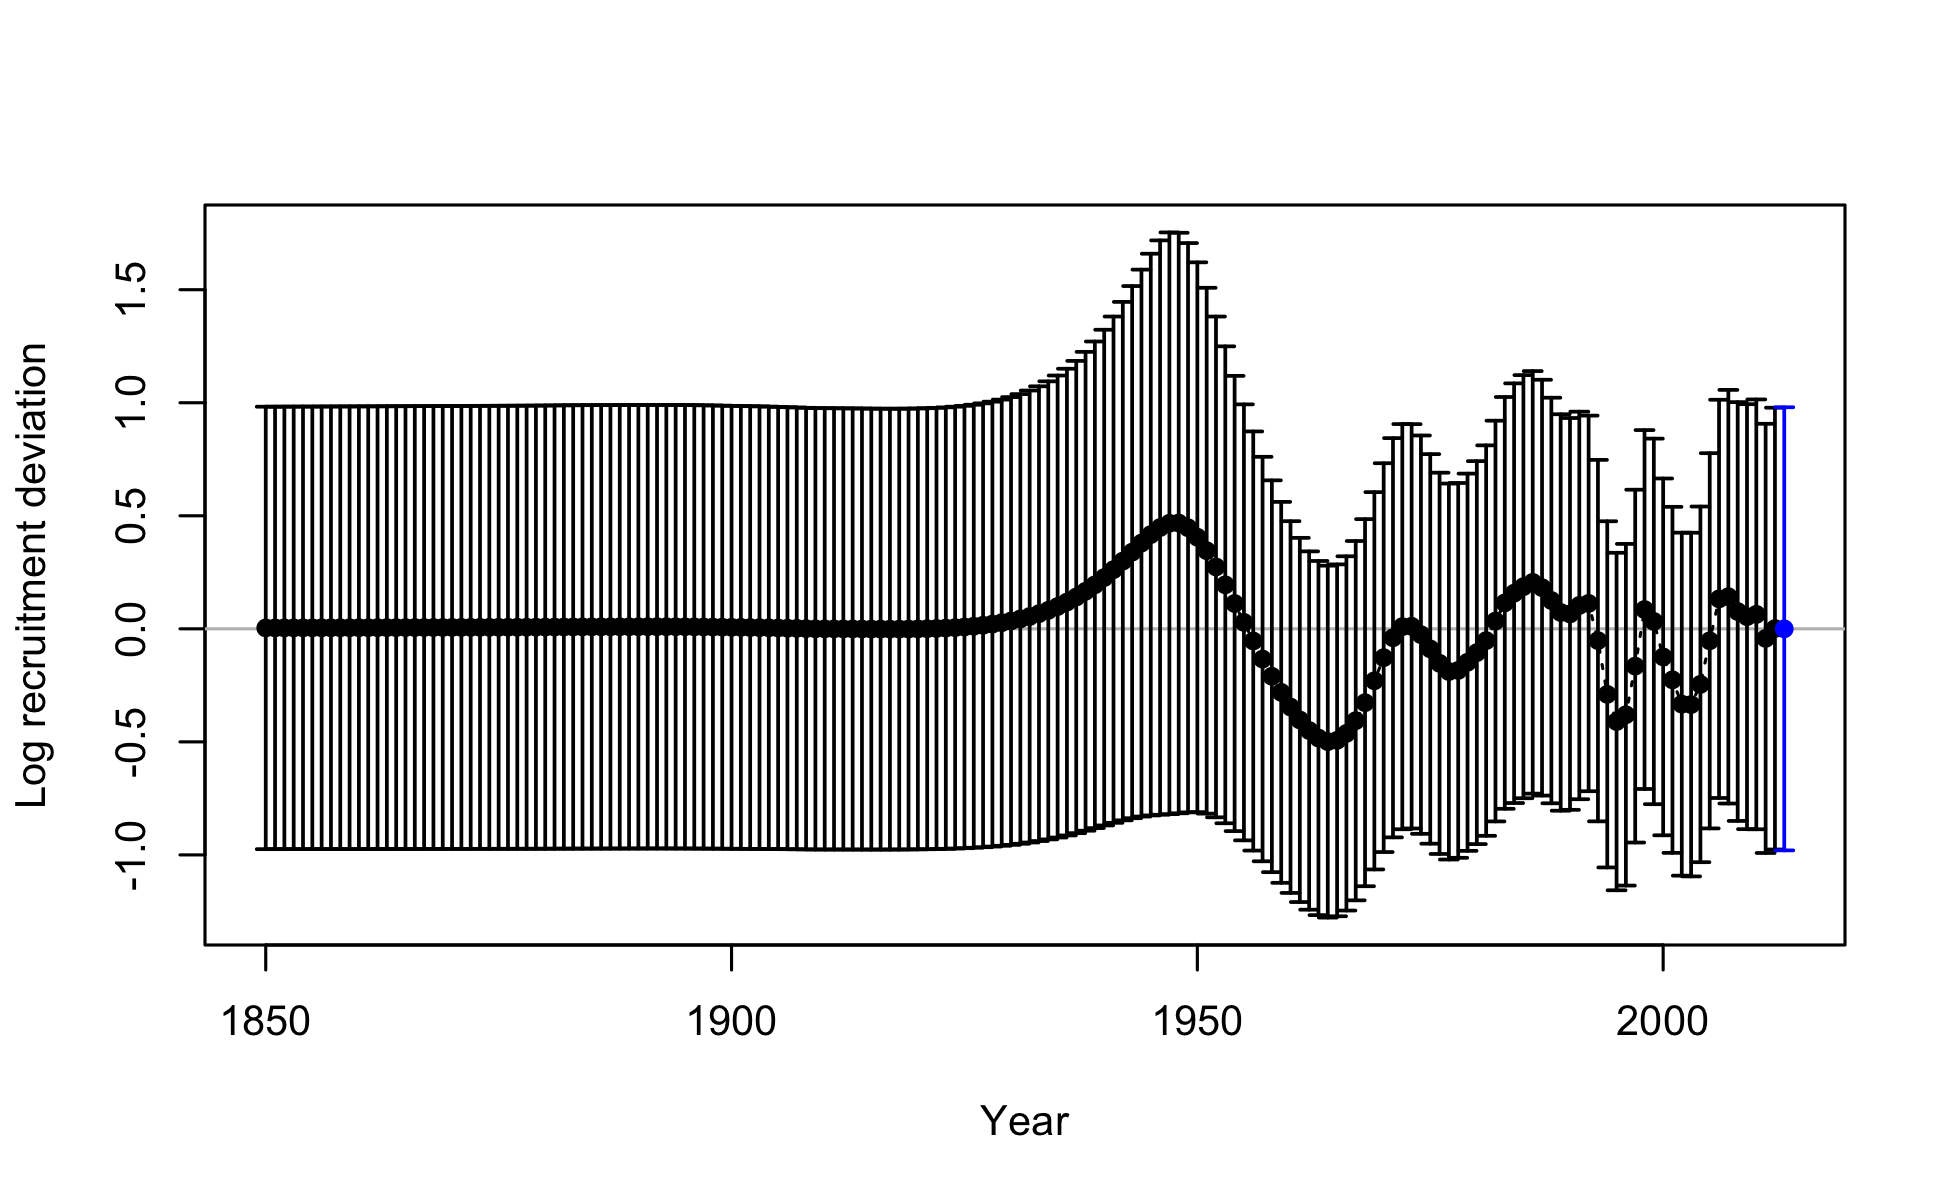
\includegraphics[width=1\textwidth,height=1\textheight]{C:/GitHub/Official_shortspine_thornyhead_2023/doc/FinalFigs/Base/recdevs2_withbars.png}
\caption{Annual recruitment deviations with 95\% intervals.\label{fig:recdevs}}
\end{figure}

\begin{figure}
\centering
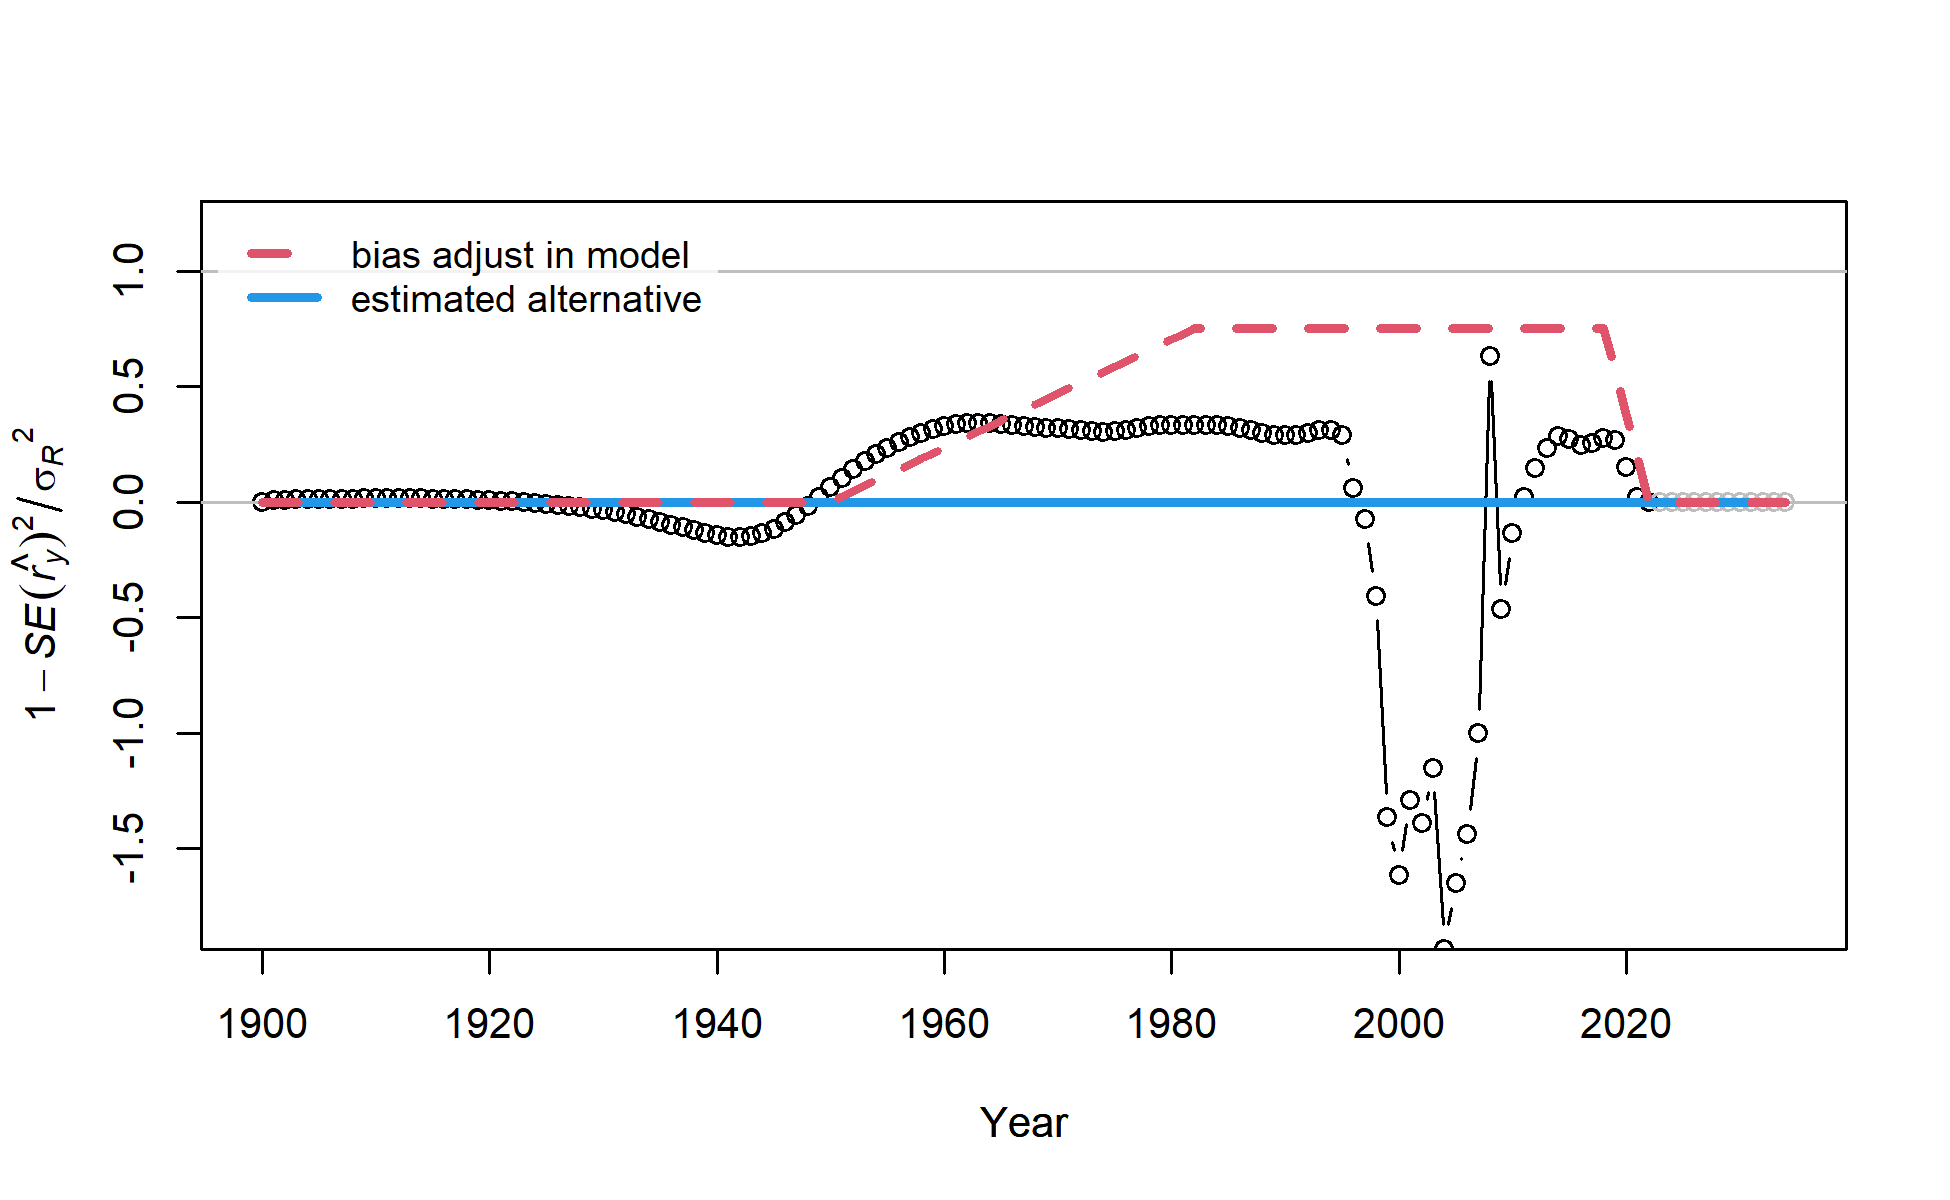
\includegraphics[width=1\textwidth,height=1\textheight]{C:/GitHub/Official_shortspine_thornyhead_2023/doc/FinalFigs/Base/recruit_fit_bias_adjust.png}
\caption{Recommended bias adjustment for recruitment deviations, from Hamel and Cope (2022).\label{fig:recdevs_bias_adjust}}
\end{figure}

\begin{figure}
\centering
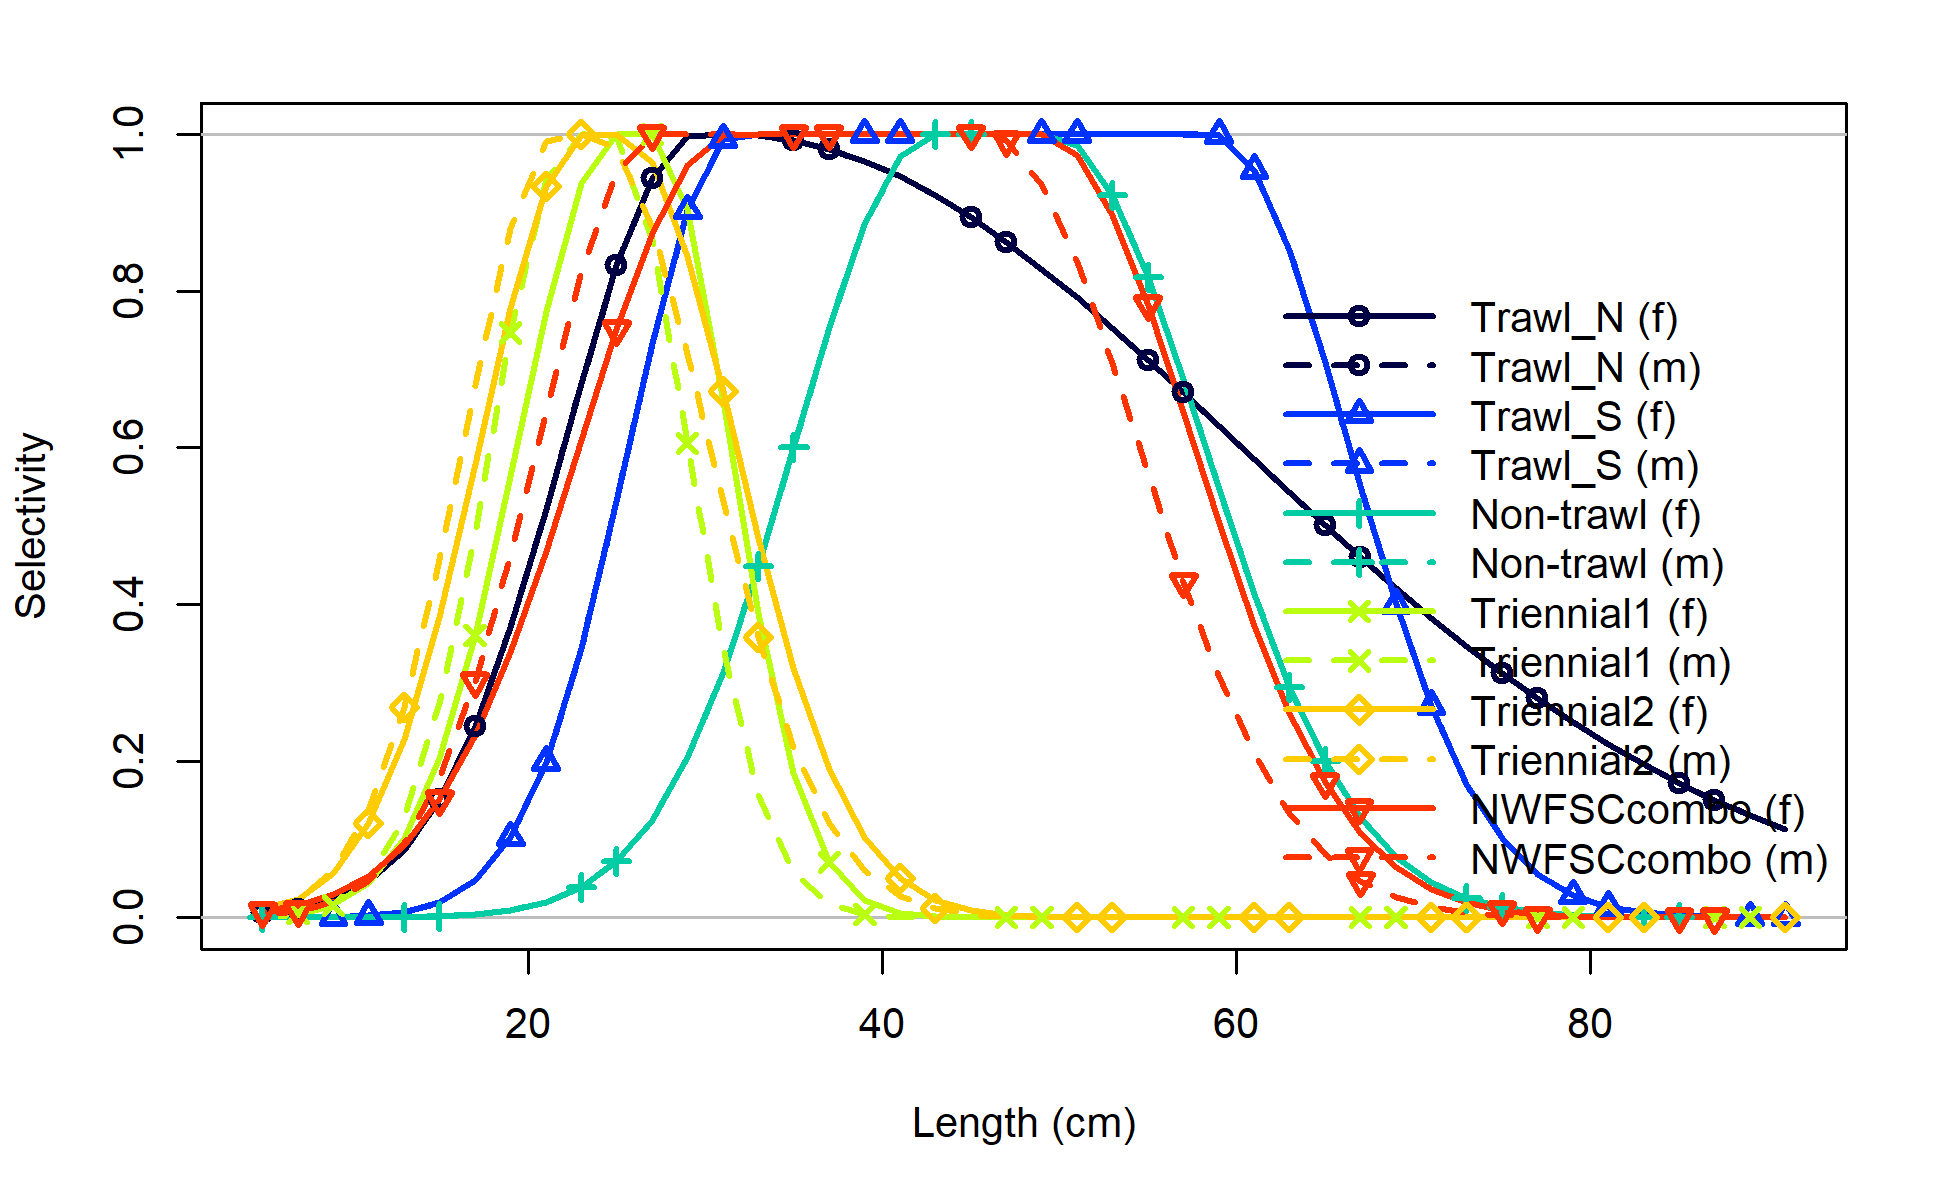
\includegraphics[width=1\textwidth,height=1\textheight]{C:/GitHub/Official_shortspine_thornyhead_2023/doc/FinalFigs/Base/sel01_multiple_fleets_length1.png}
\caption{Selectivity at length for each combination of sex and fleet. Note that the three commerical fishery fleets were not modeled as having sex-specific selectivity.\label{fig:selcurvs}}
\end{figure}

\begin{figure}
\centering
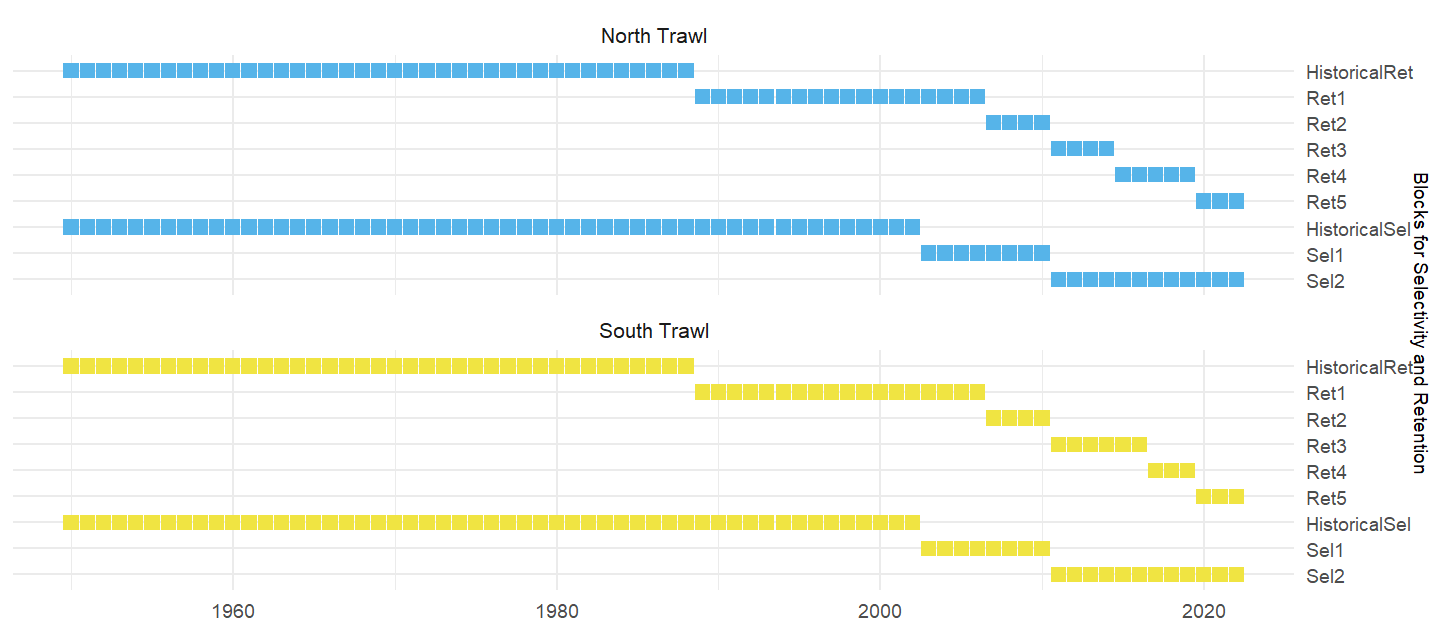
\includegraphics[width=1\textwidth,height=1\textheight]{C:/GitHub/Official_shortspine_thornyhead_2023/doc/FinalFigs/Sensitivities/Selectivity/timeblocks2.png}
\caption{Time blocking for selectivity and retention for North and South trawl fleets.\label{fig:timeblocks}}
\end{figure}

\begin{figure}
\centering
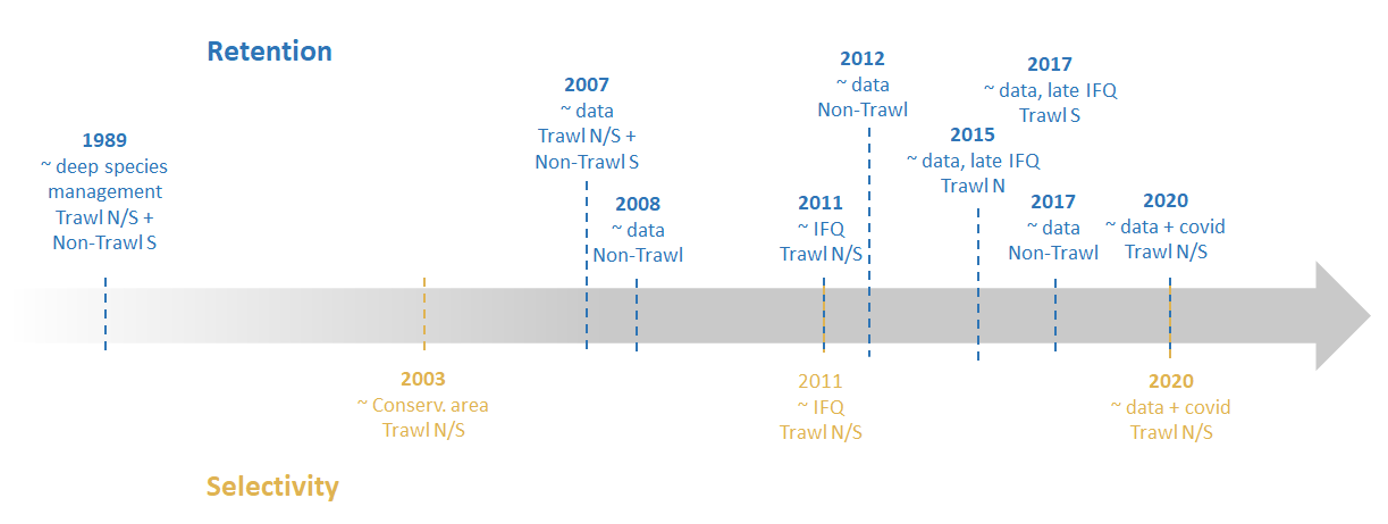
\includegraphics[width=1\textwidth,height=1\textheight]{C:/GitHub/Official_shortspine_thornyhead_2023/doc/FinalFigs/Base/blockingdiagram.png}
\caption{Timeline of management and fleet behavior changes associated with selectivity and retention blocks.\label{fig:diagram}}
\end{figure}

\begin{figure}
\centering
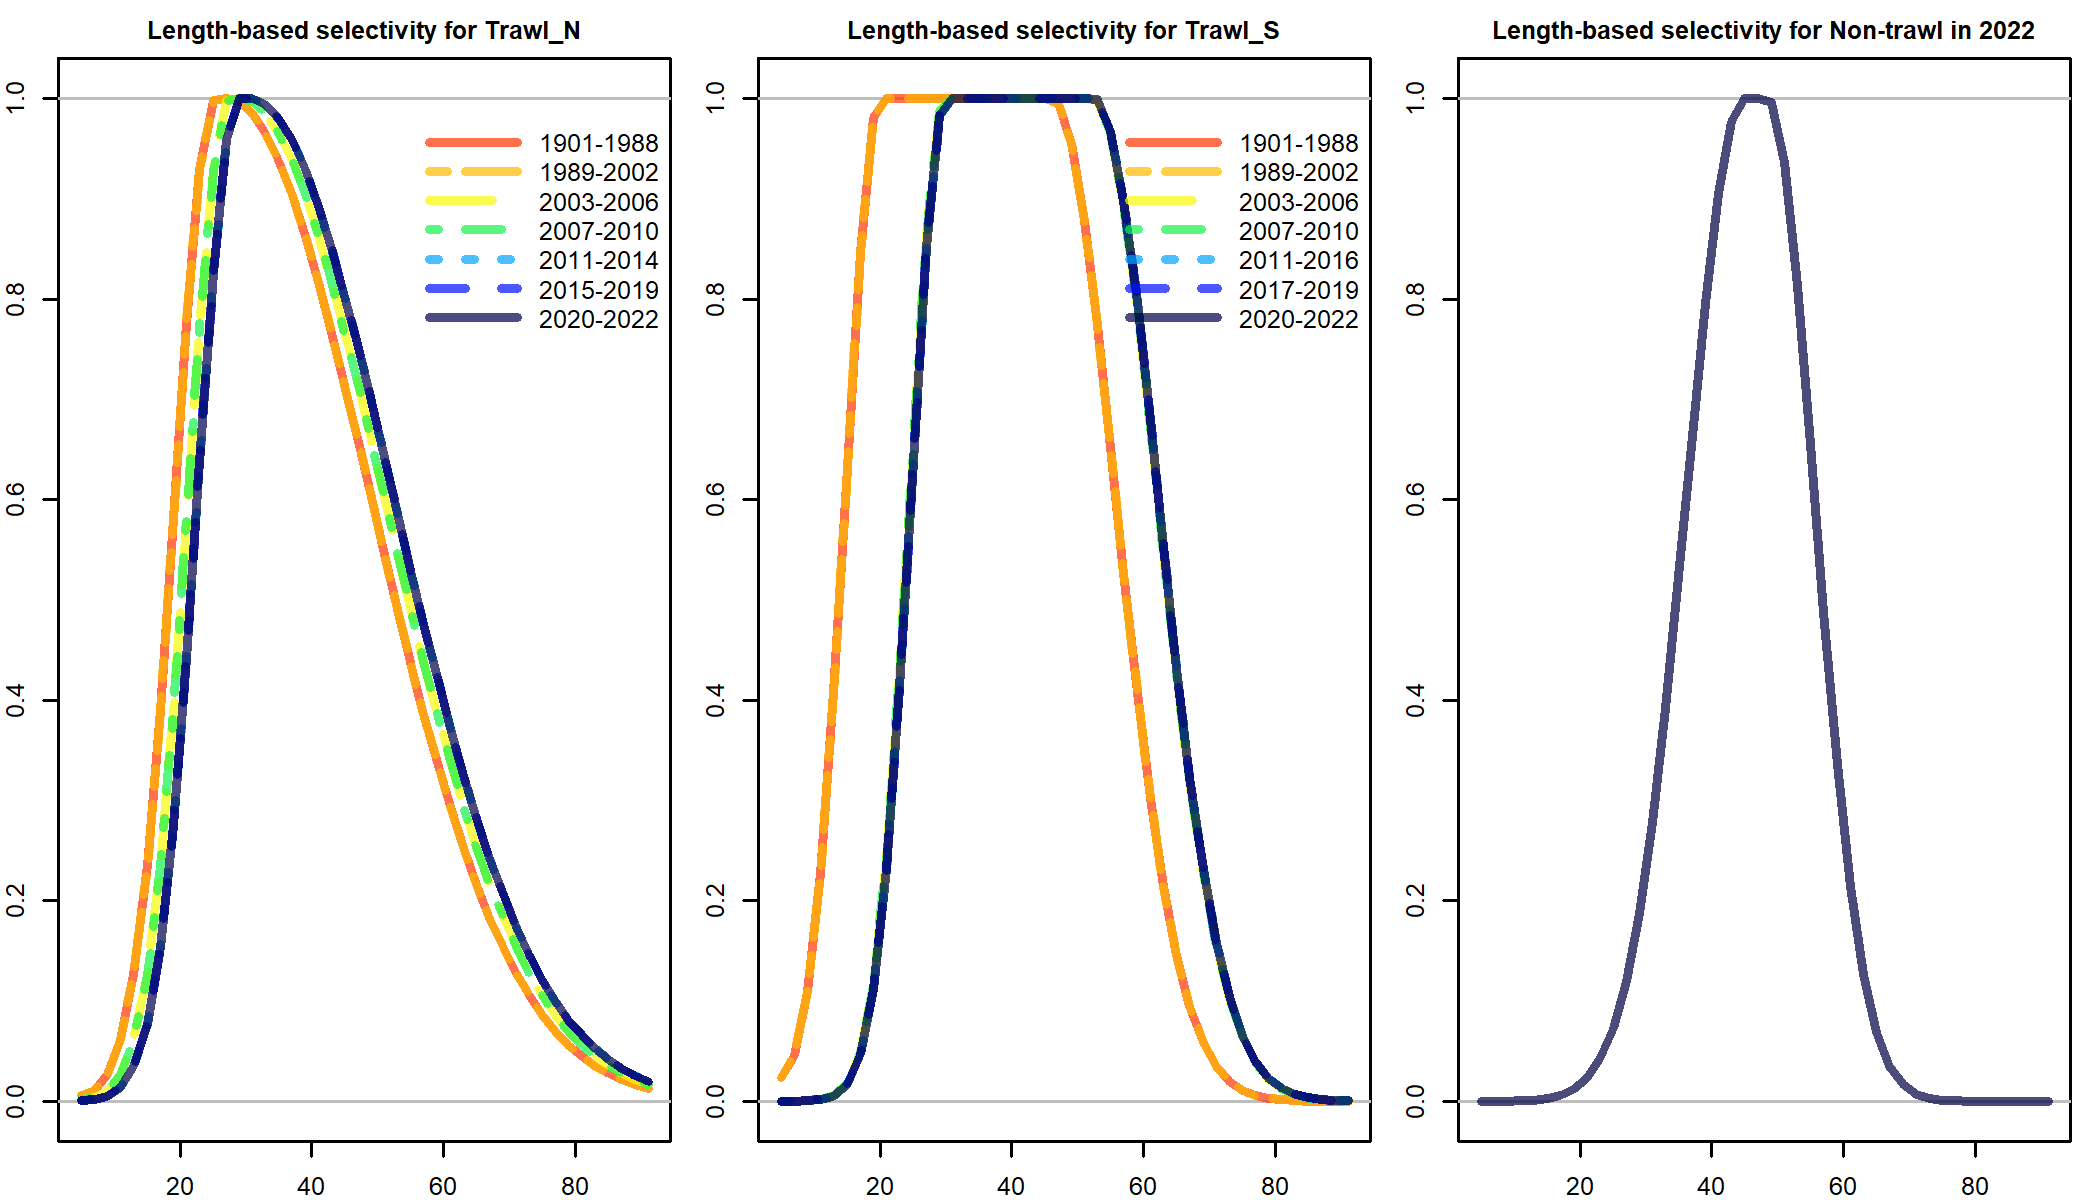
\includegraphics[width=1\textwidth,height=1\textheight]{C:/GitHub/Official_shortspine_thornyhead_2023/doc/FinalFigs/Base/selec_block.png}
\caption{Selectivity curves for time blocks in the North Trawl, South Trawl, and Non-Trawl fleets.\label{fig:selblocks}}
\end{figure}

\begin{figure}
\centering
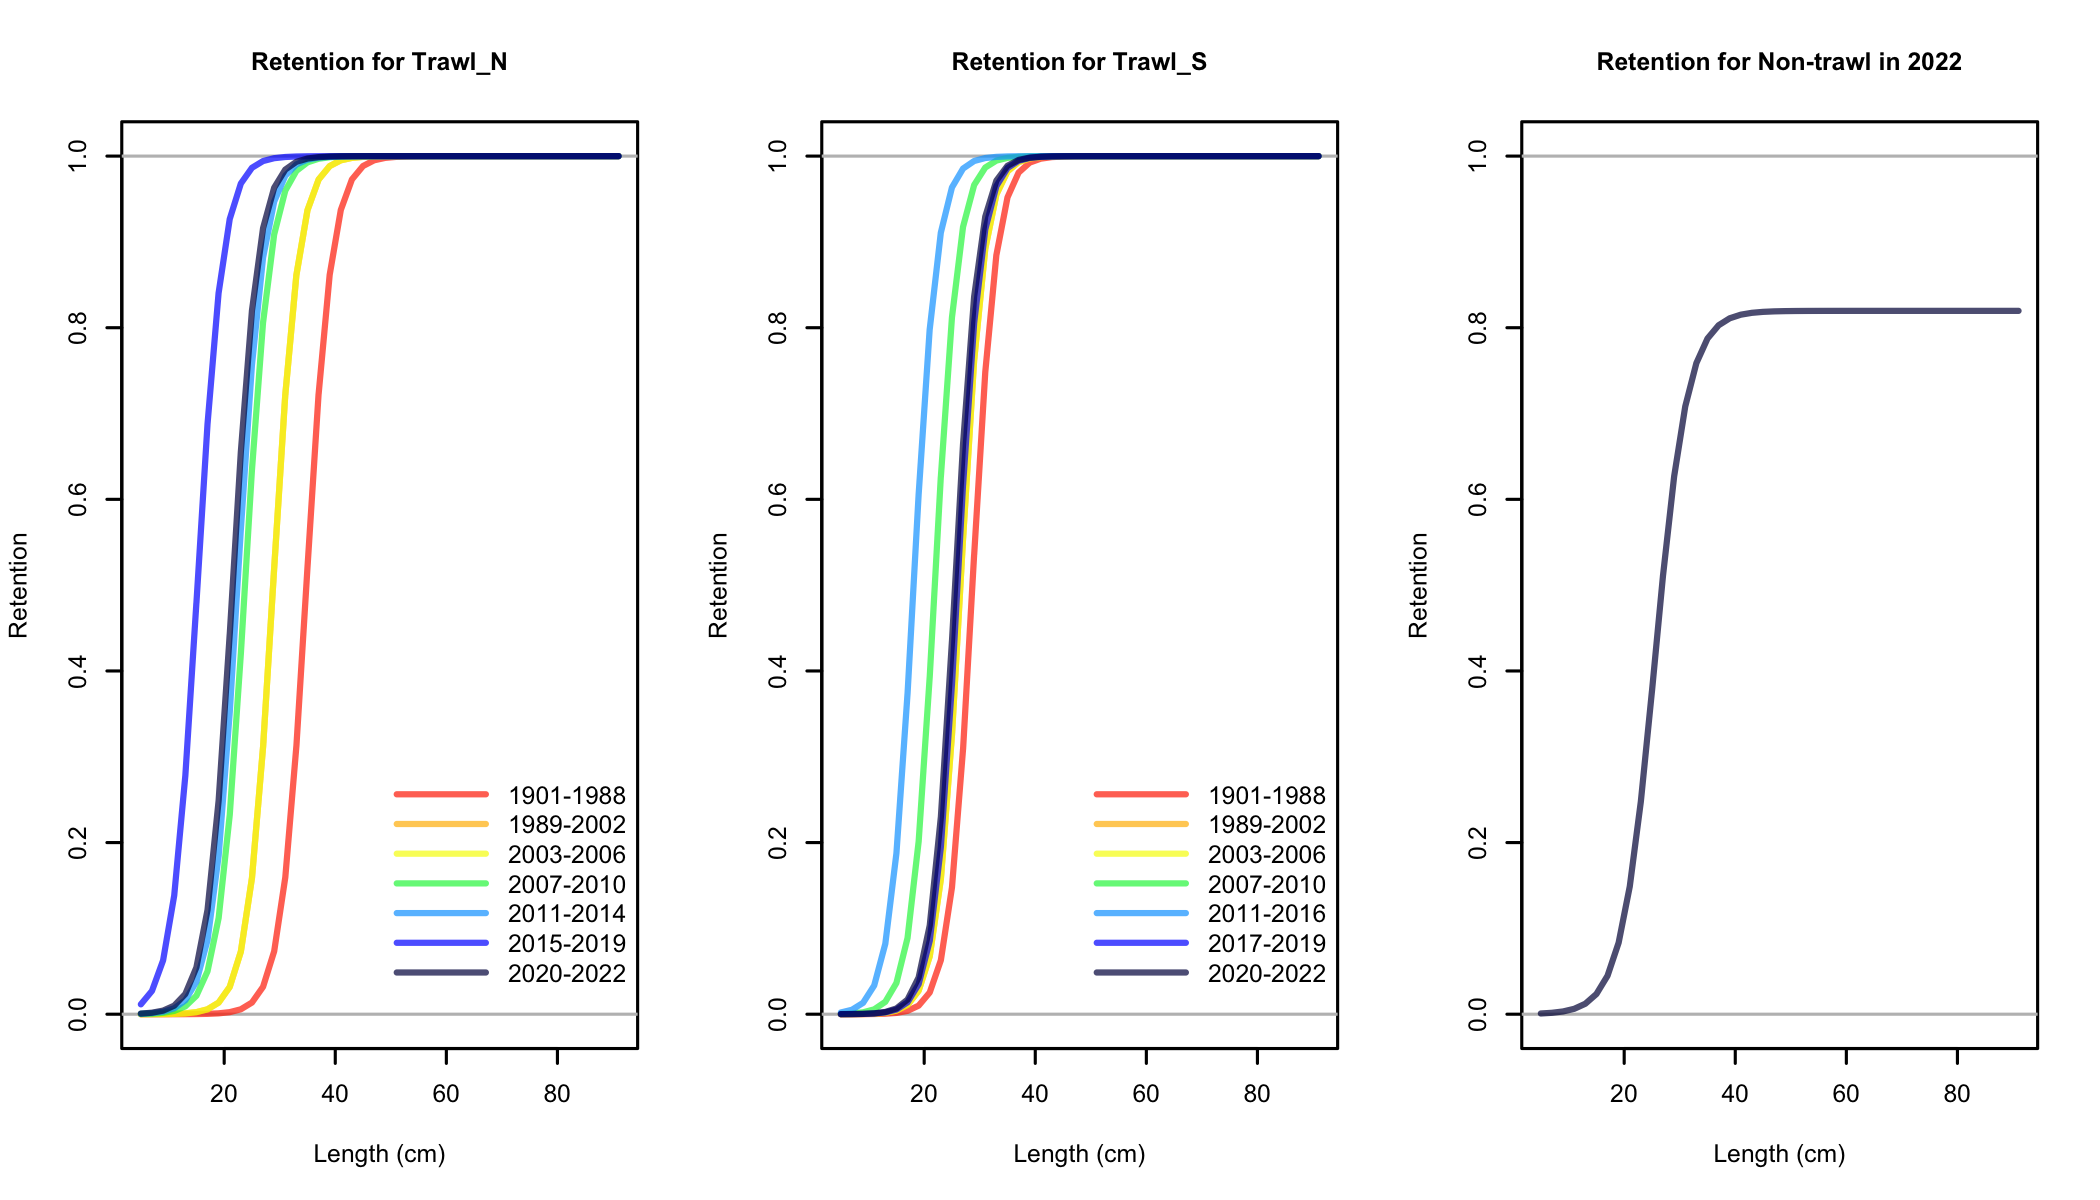
\includegraphics[width=1\textwidth,height=1\textheight]{C:/GitHub/Official_shortspine_thornyhead_2023/doc/FinalFigs/Base/retention_curves.png}
\caption{Retention curves for time blocks in the North Trawl, South Trawl, and Non-Trawl fleets.\label{fig:retblocks}}
\end{figure}

\begin{figure}
\centering
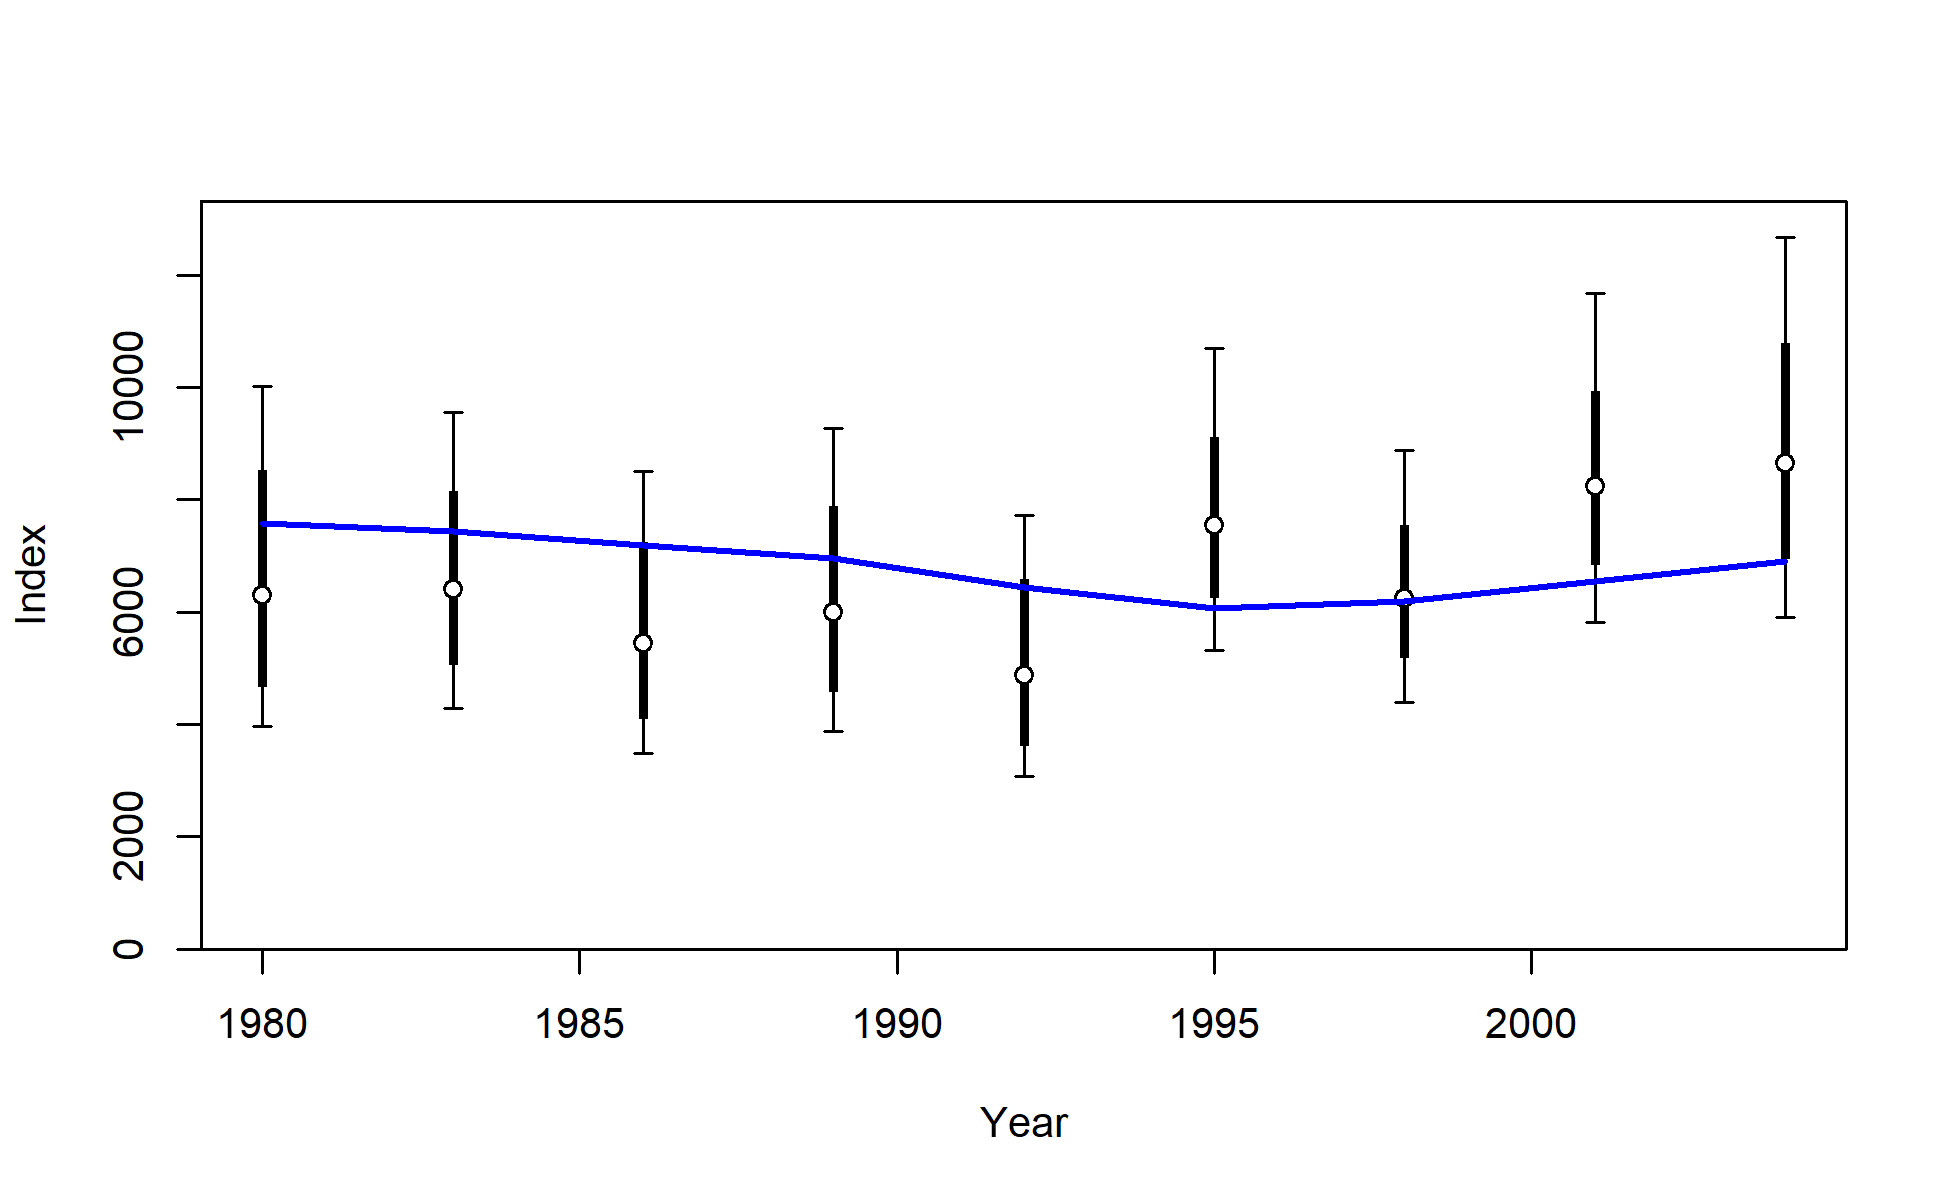
\includegraphics[width=1\textwidth,height=1\textheight]{C:/GitHub/Official_shortspine_thornyhead_2023/doc/FinalFigs/Base/index2_cpuefit_Triennial1.png}
\caption{Fit to index of abundance data for the Triennial Survey. Lines indicate 95\% uncertainty interval around index values based on the model assumption of lognormal error. Thicker lines indicate input uncertainty before addition of estimated additional uncertainty parameter.\label{fig:fitsTri1}}
\end{figure}

\begin{figure}
\centering
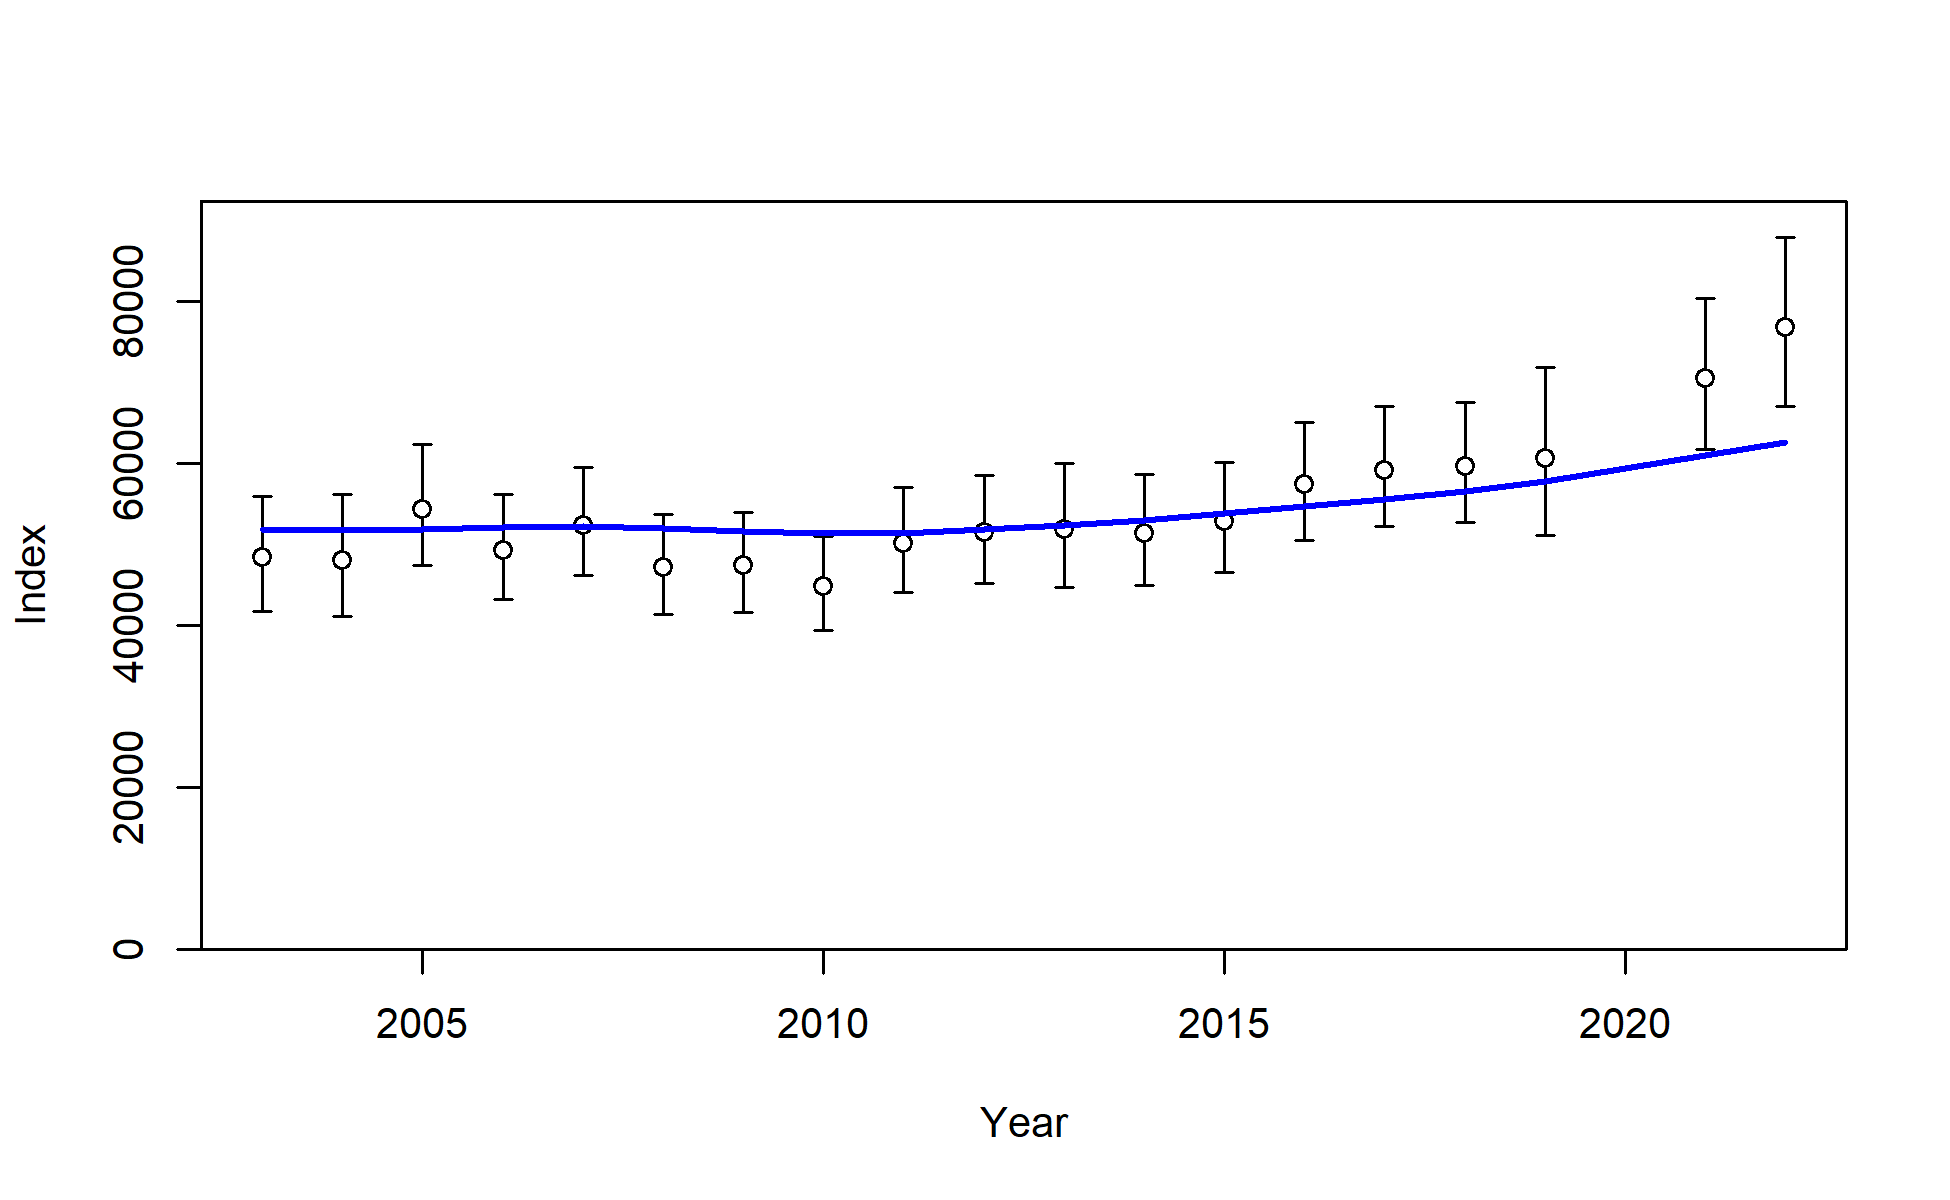
\includegraphics[width=1\textwidth,height=1\textheight]{C:/GitHub/Official_shortspine_thornyhead_2023/doc/FinalFigs/Base/index2_cpuefit_NWFSCcombo.png}
\caption{Fit to index of abundance data for the WCGBTS. Lines indicate 95\% uncertainty interval around index values based on the model assumption of lognormal error. Thicker lines indicate input uncertainty before addition of estimated additional uncertainty parameter.\label{fig:fitscombo}}
\end{figure}

\begin{figure}
\centering
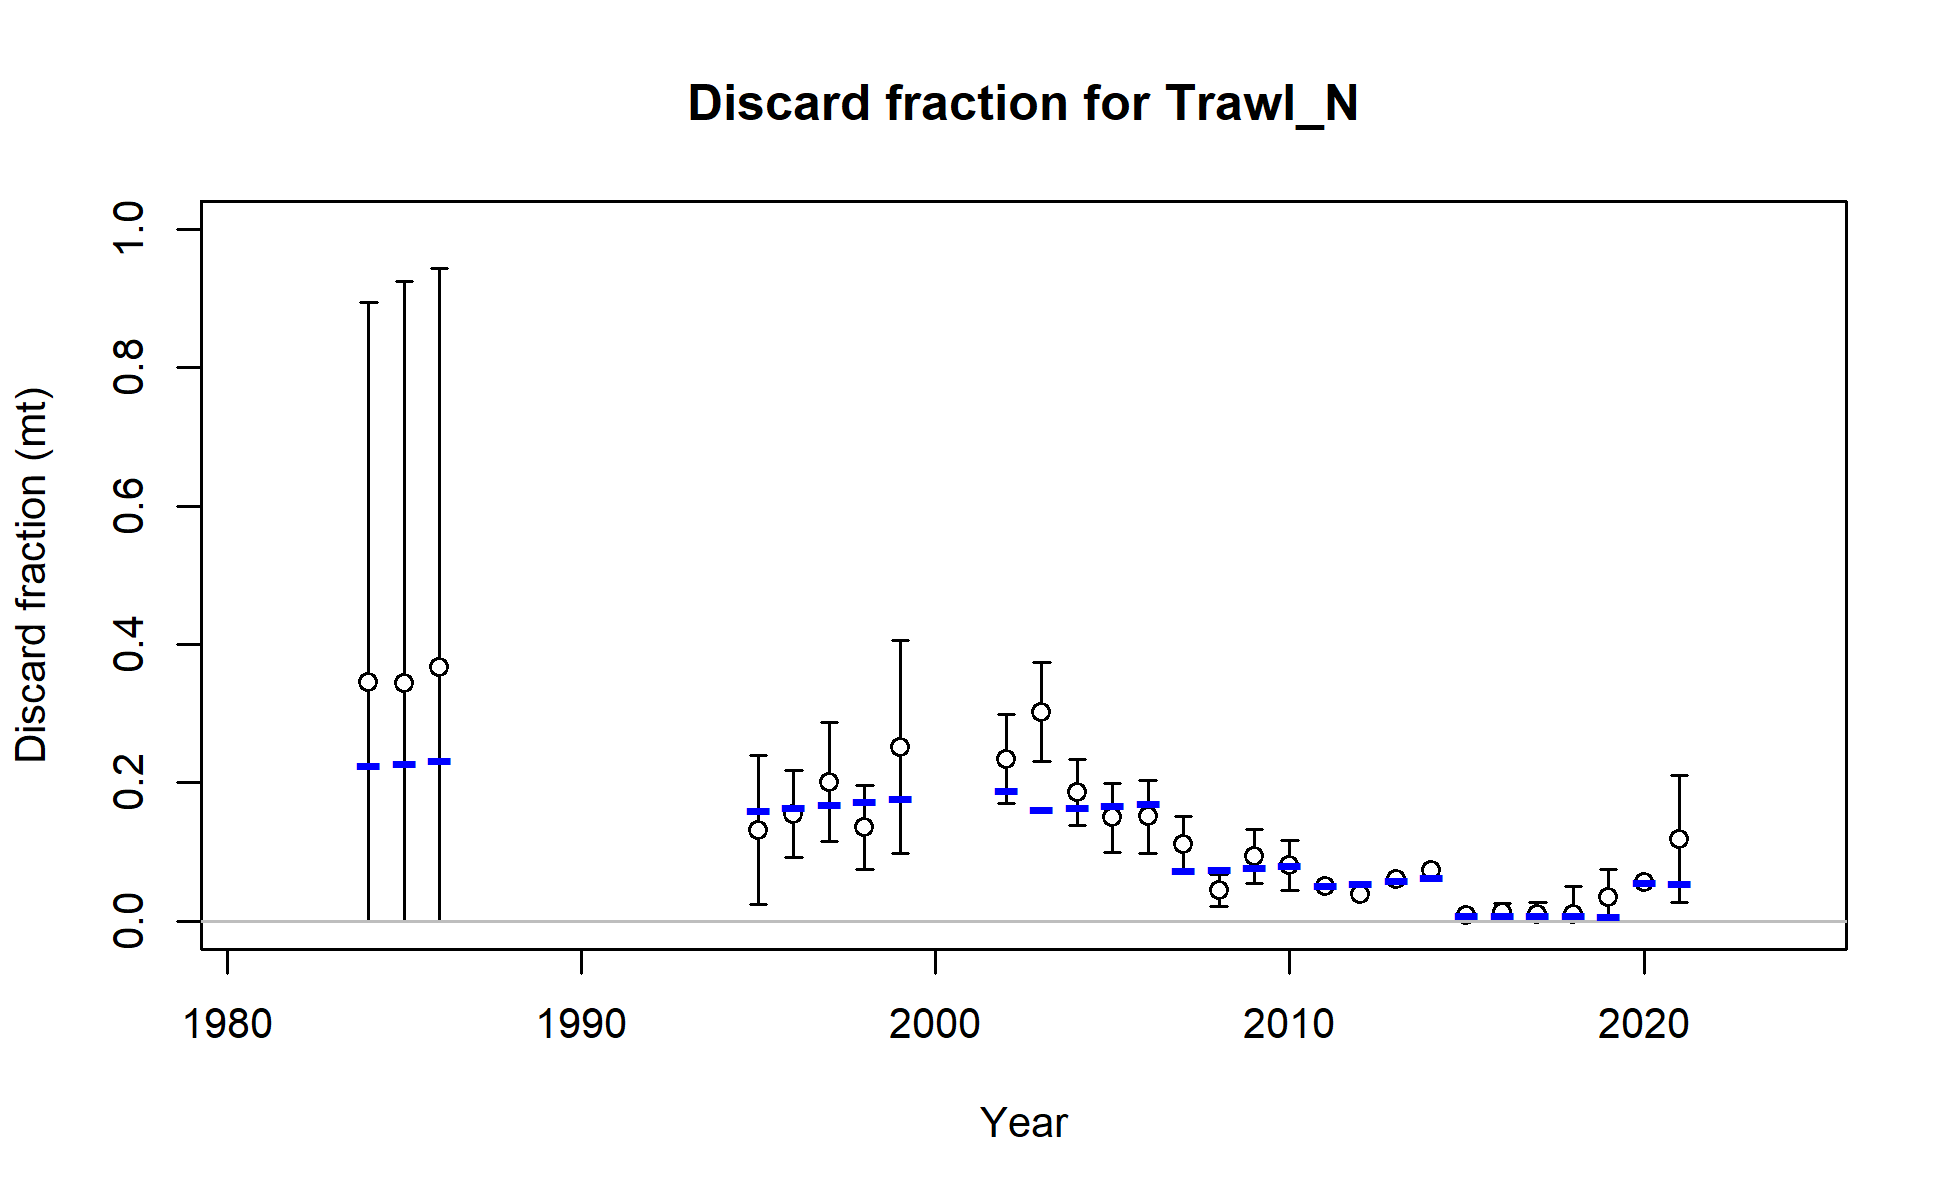
\includegraphics[width=1\textwidth,height=1\textheight]{C:/GitHub/Official_shortspine_thornyhead_2023/doc/FinalFigs/Base/discard_fitTrawl_N.png}
\caption{Discard fraction (percent of total catch that is not landed) for the North trawl fleet.\label{fig:northtrl_disc}}
\end{figure}

\begin{figure}
\centering
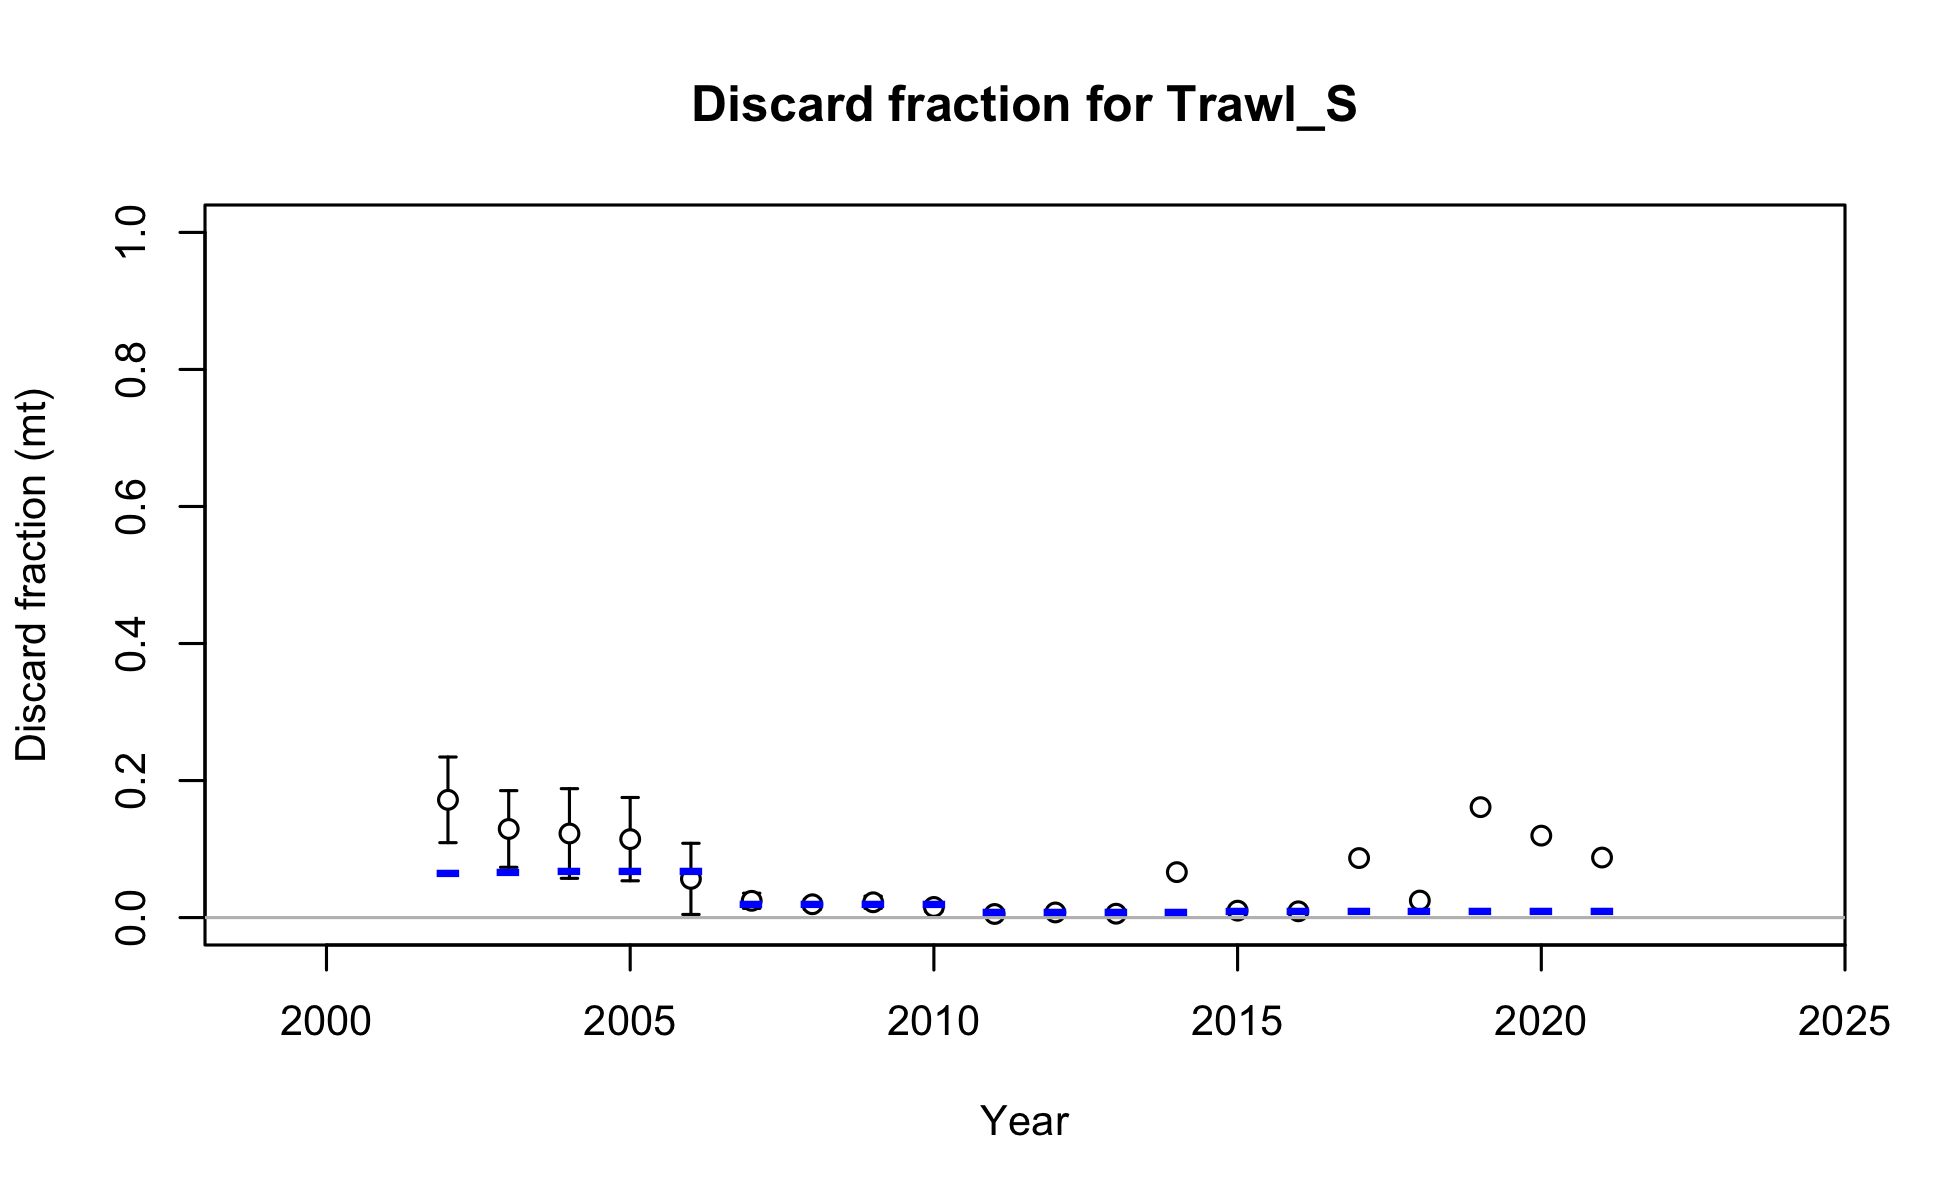
\includegraphics[width=1\textwidth,height=1\textheight]{C:/GitHub/Official_shortspine_thornyhead_2023/doc/FinalFigs/Base/discard_fitTrawl_S.png}
\caption{Discard fraction (percent of total catch that is not landed) for the South trawl fleet.\label{fig:southtrl_disc}}
\end{figure}

\begin{figure}
\centering
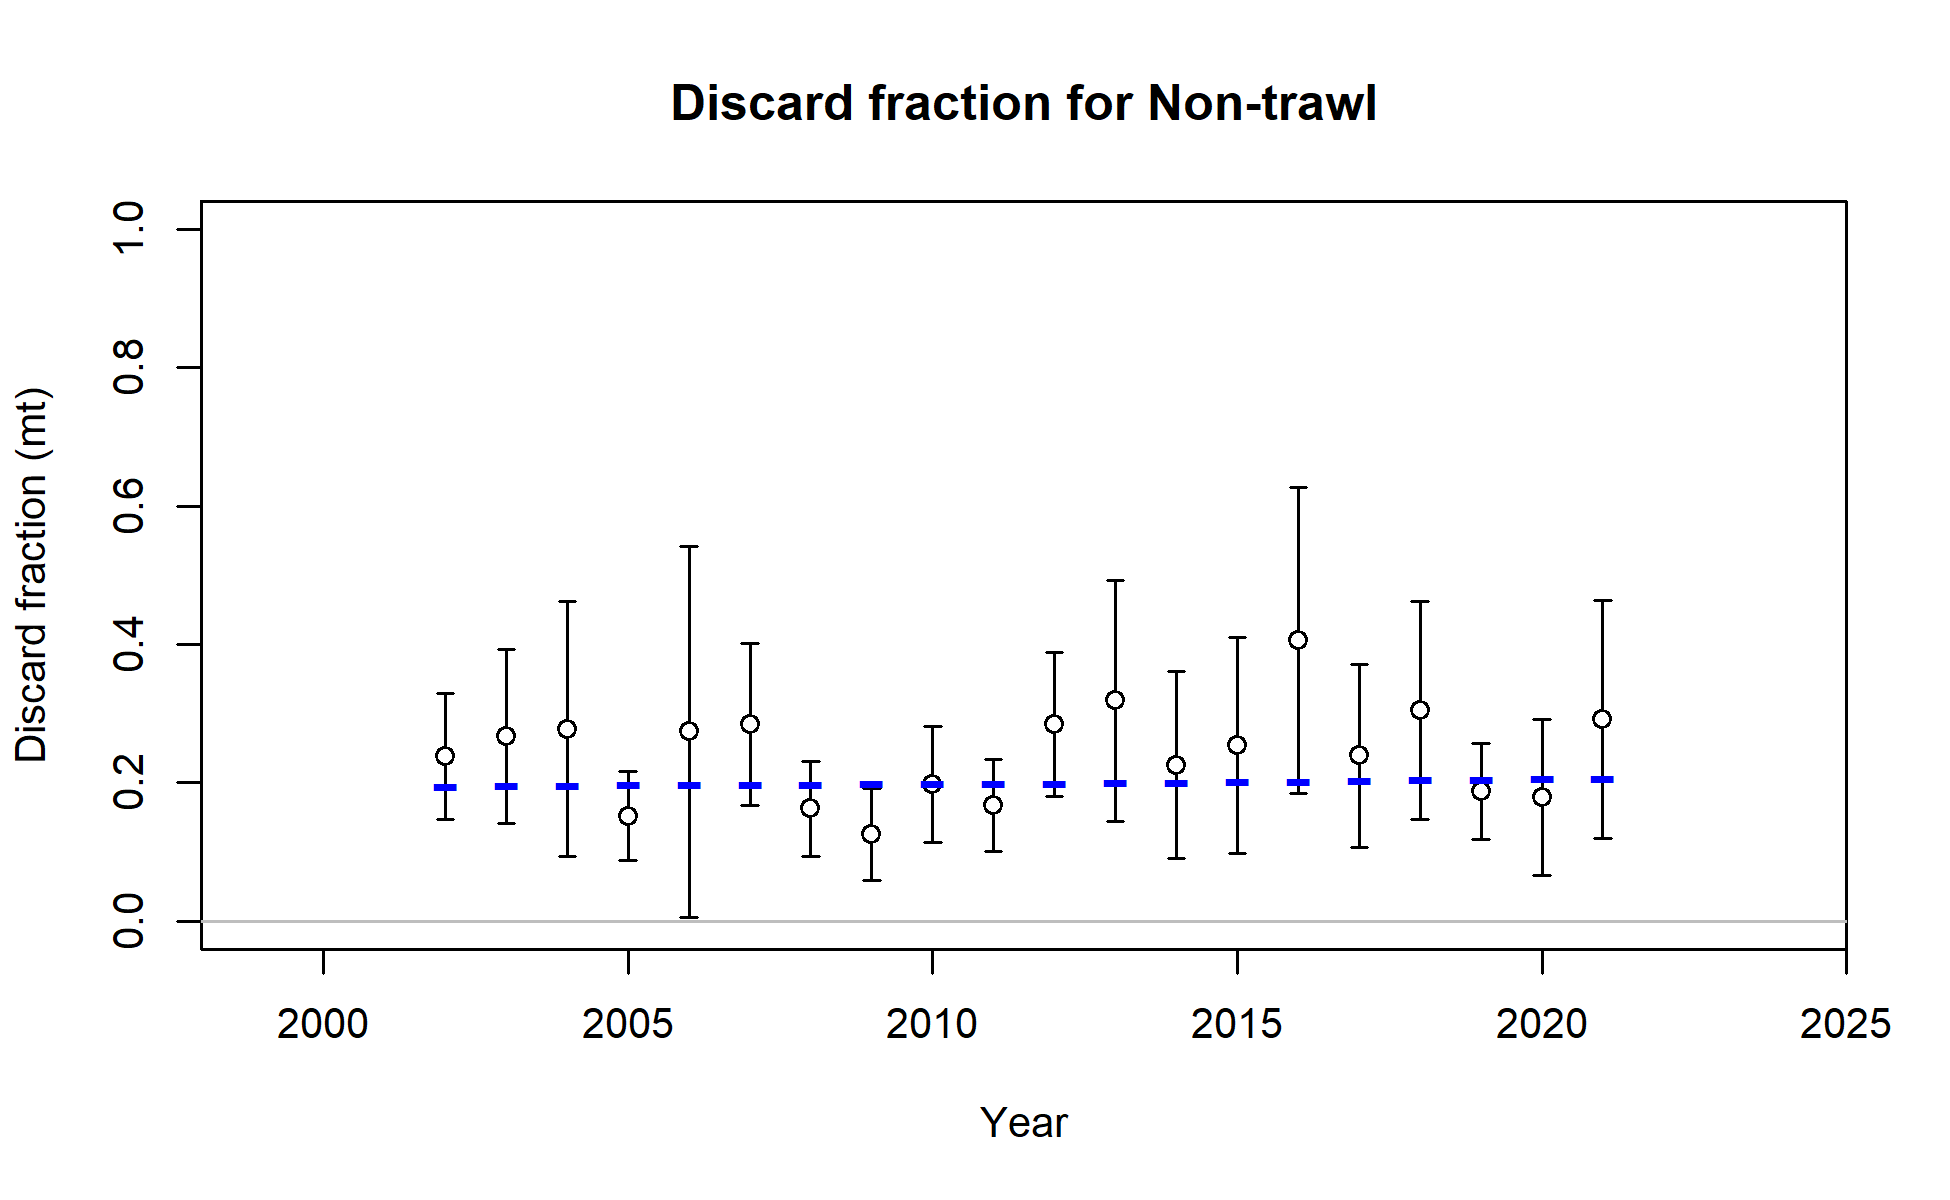
\includegraphics[width=1\textwidth,height=1\textheight]{C:/GitHub/Official_shortspine_thornyhead_2023/doc/FinalFigs/Base/discard_fitNon-trawl.png}
\caption{Discard fraction (percent of total catch that is not landed) for the Non-trawl fleet.\label{fig:nontrl_disc}}
\end{figure}

\begin{figure}
\centering
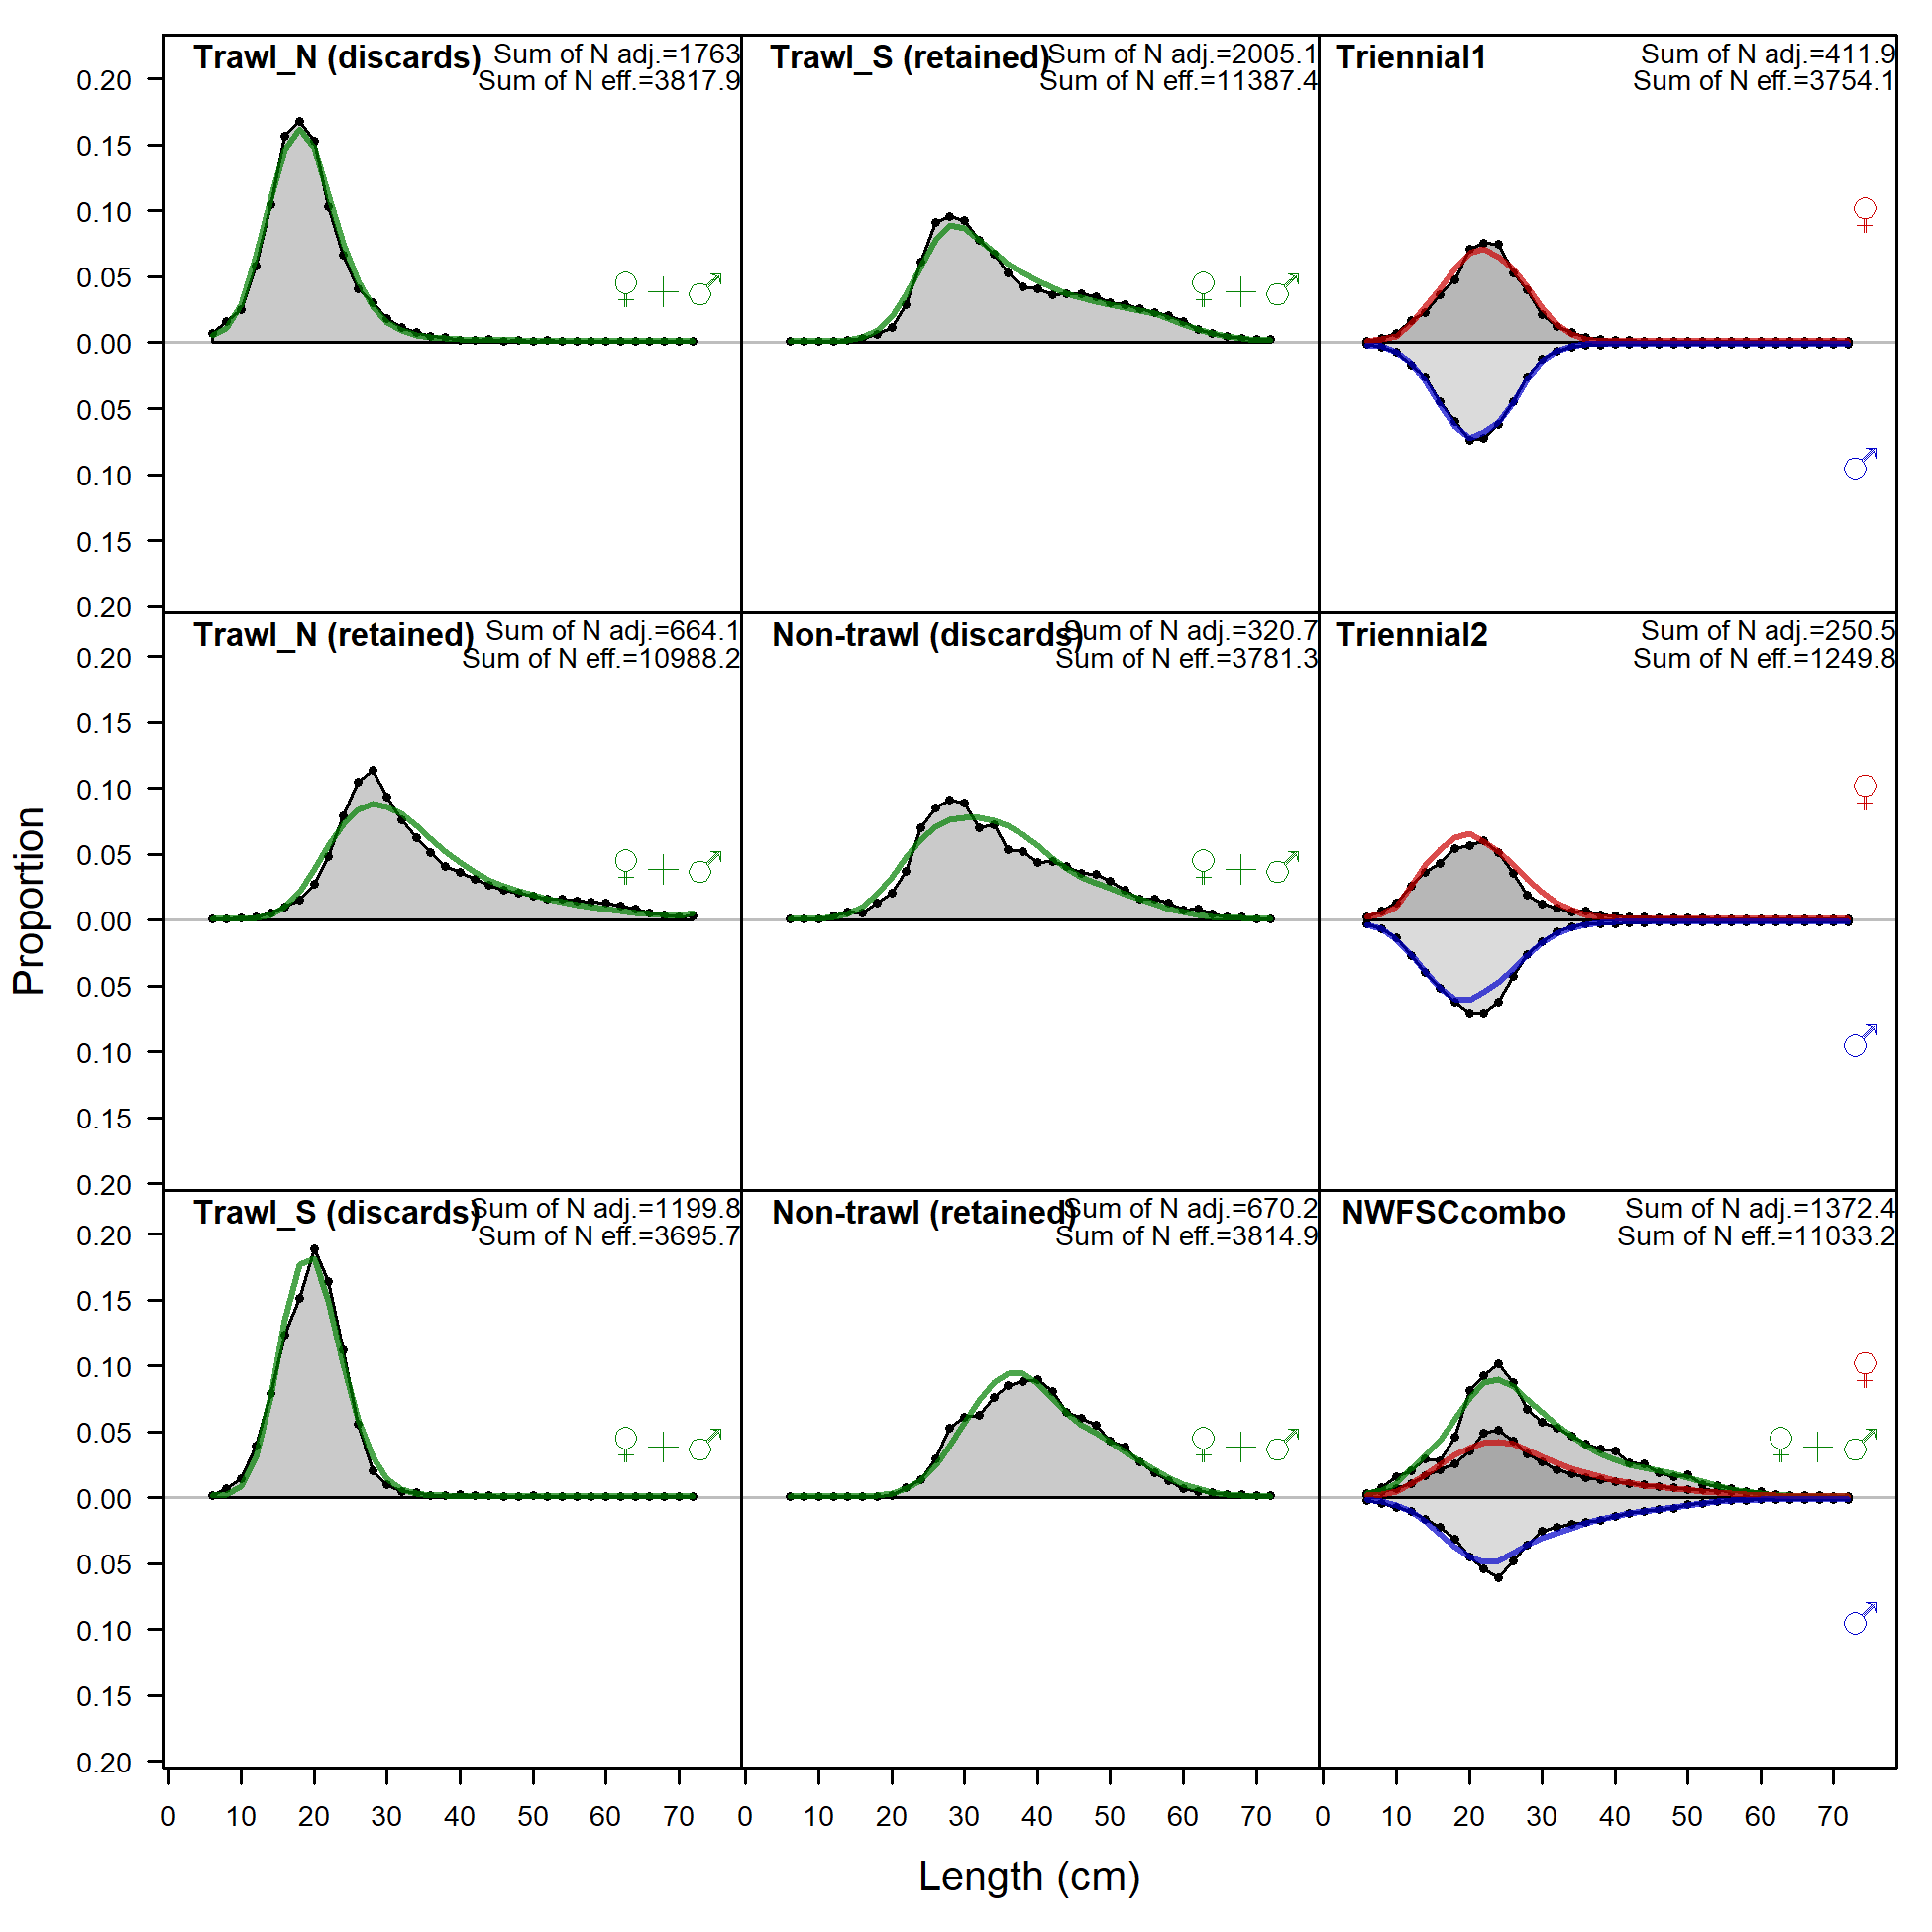
\includegraphics[width=1\textwidth,height=1\textheight]{C:/GitHub/Official_shortspine_thornyhead_2023/doc/FinalFigs/Base/comp_lenfit__aggregated_across_time.png}
\caption{Length comps, aggregated across time by fleet. Labels `retained' and `discard' indicate discarded or retained samples for each fleet. Panels without this designation represent the whole catch.\label{fig:lencomps_all}}
\end{figure}

\begin{figure}
\centering
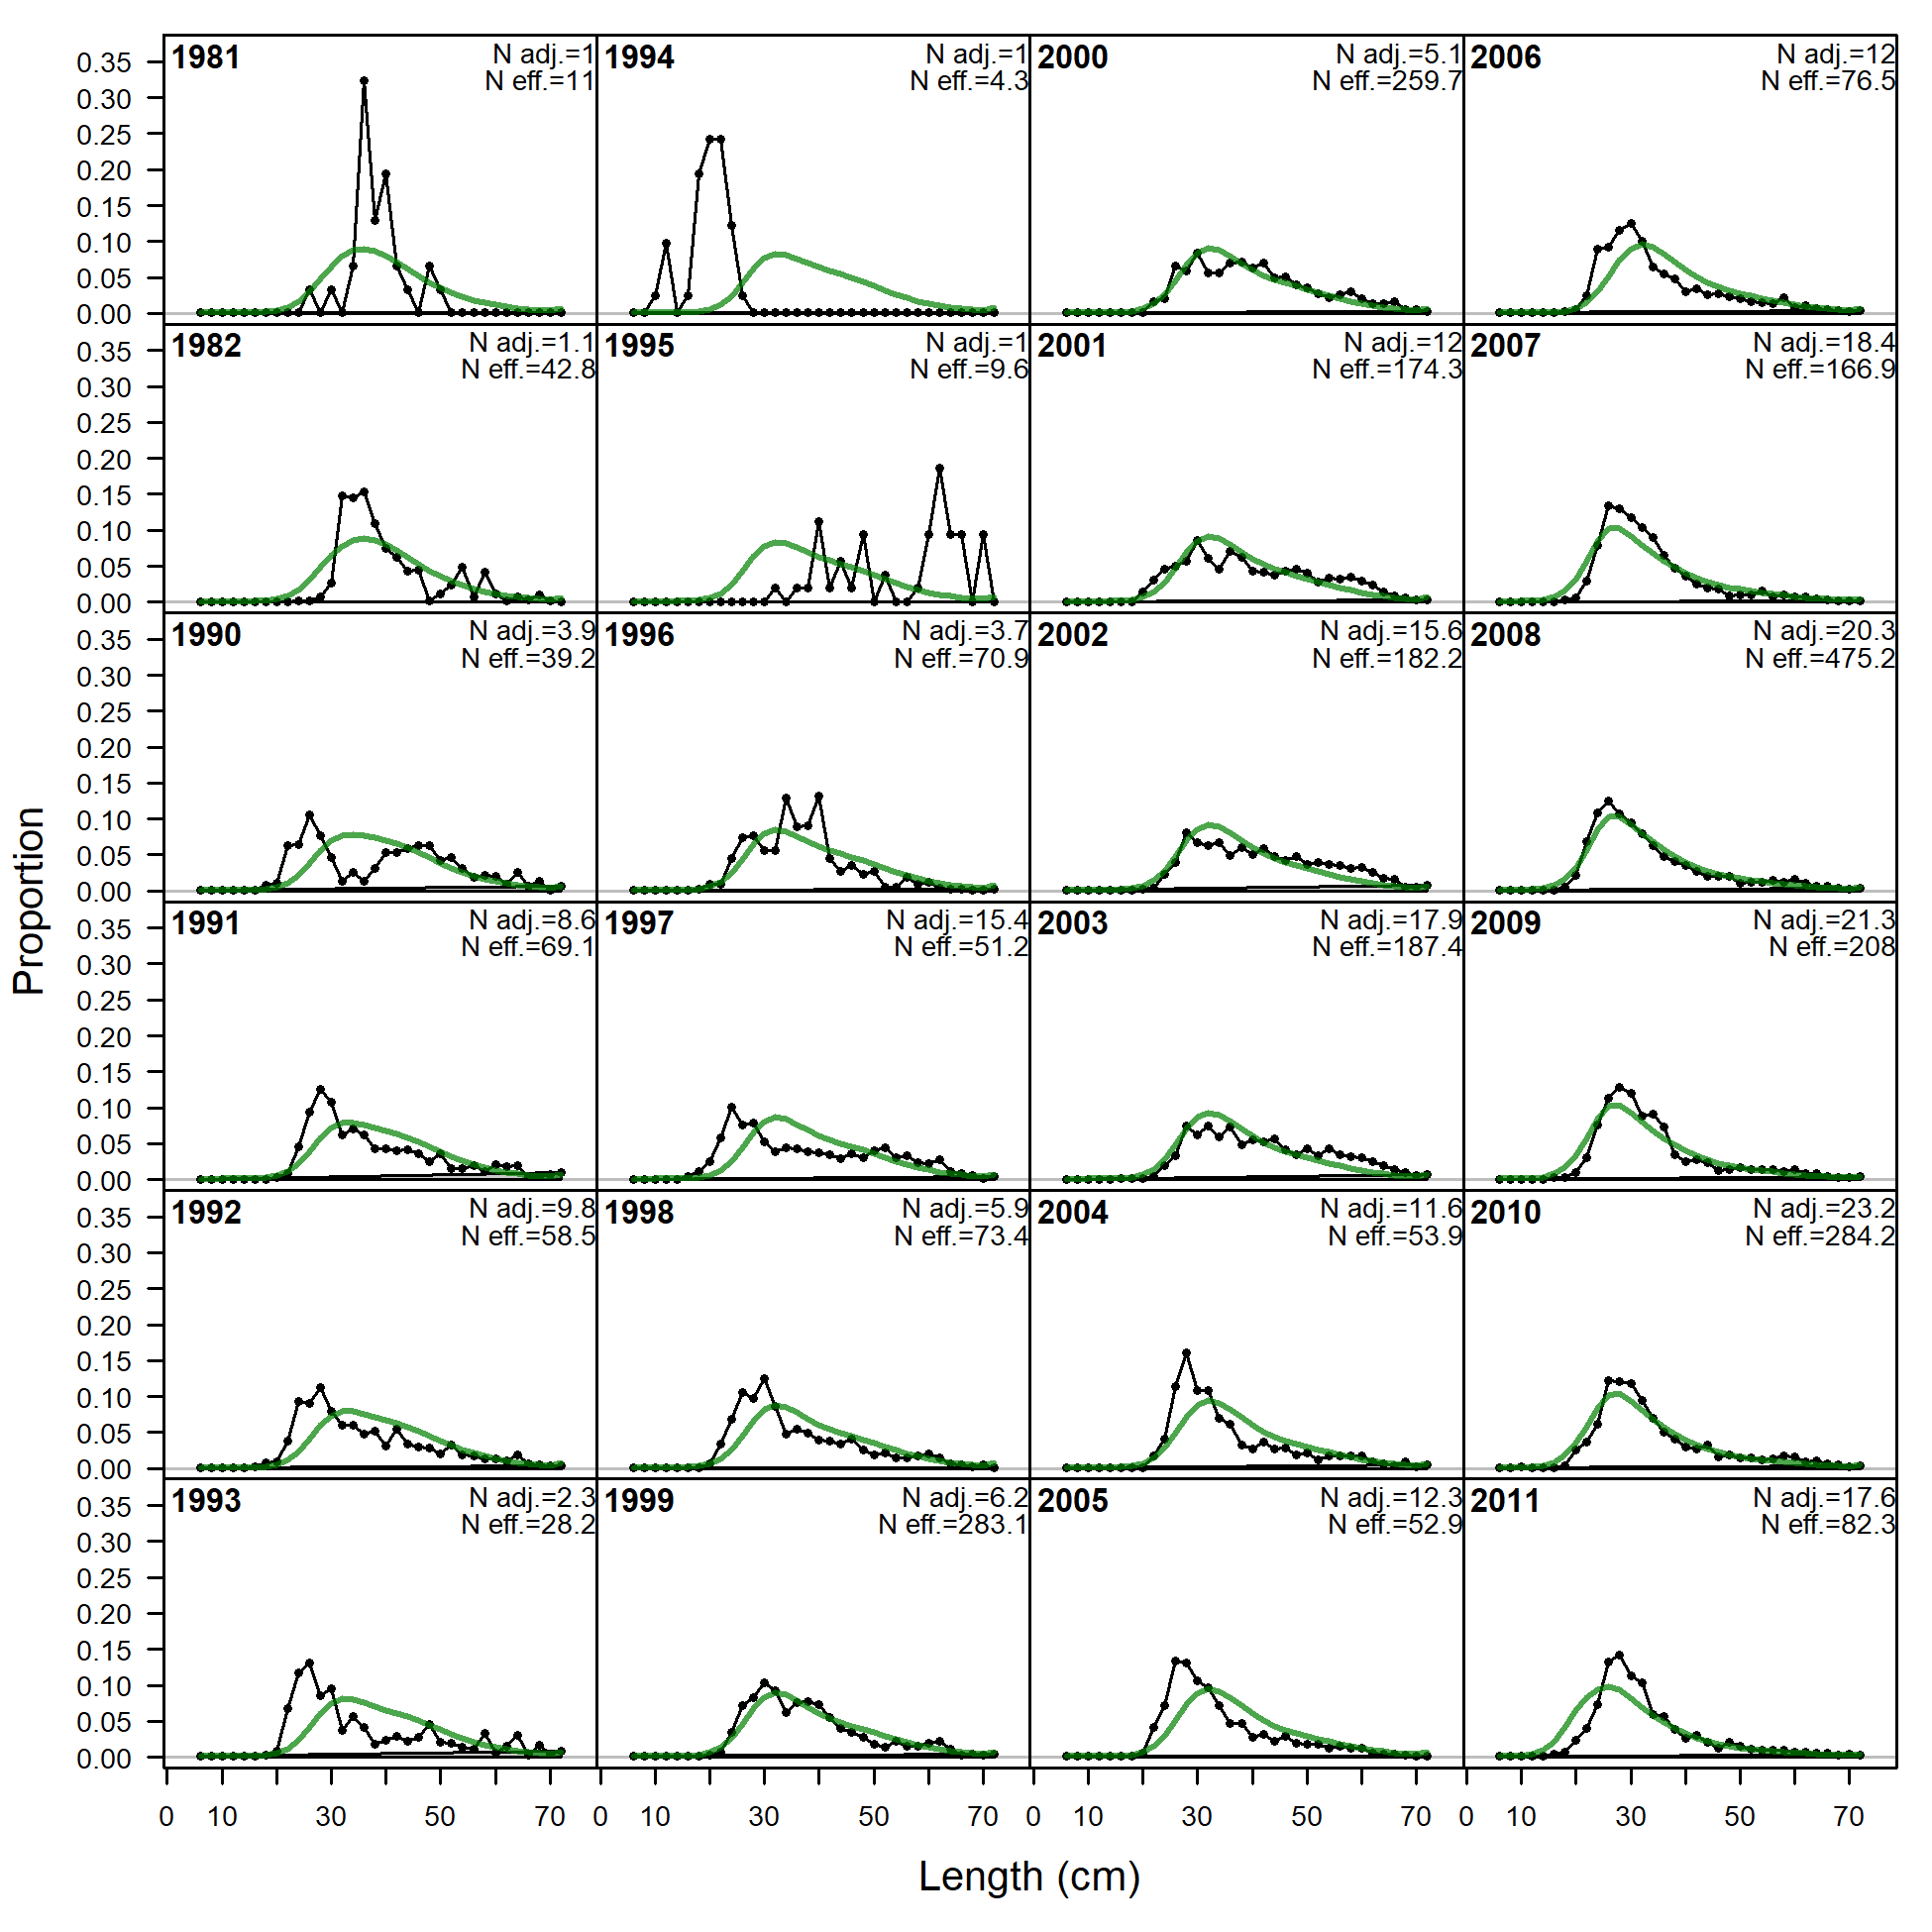
\includegraphics[width=1\textwidth,height=1\textheight]{C:/GitHub/Official_shortspine_thornyhead_2023/doc/FinalFigs/Base/comp_lenfit_flt1mkt2_page1.png}
\caption{Annual length comps and model fit for North trawl retained catch. `N adj.' is the input sample size after data-weighting adjustment. N eff. is the calculated effective sample size used in the McAllister-Ianelli tuning method.\label{fig:ntrawl_comps_1}}
\end{figure}

\begin{figure}
\centering
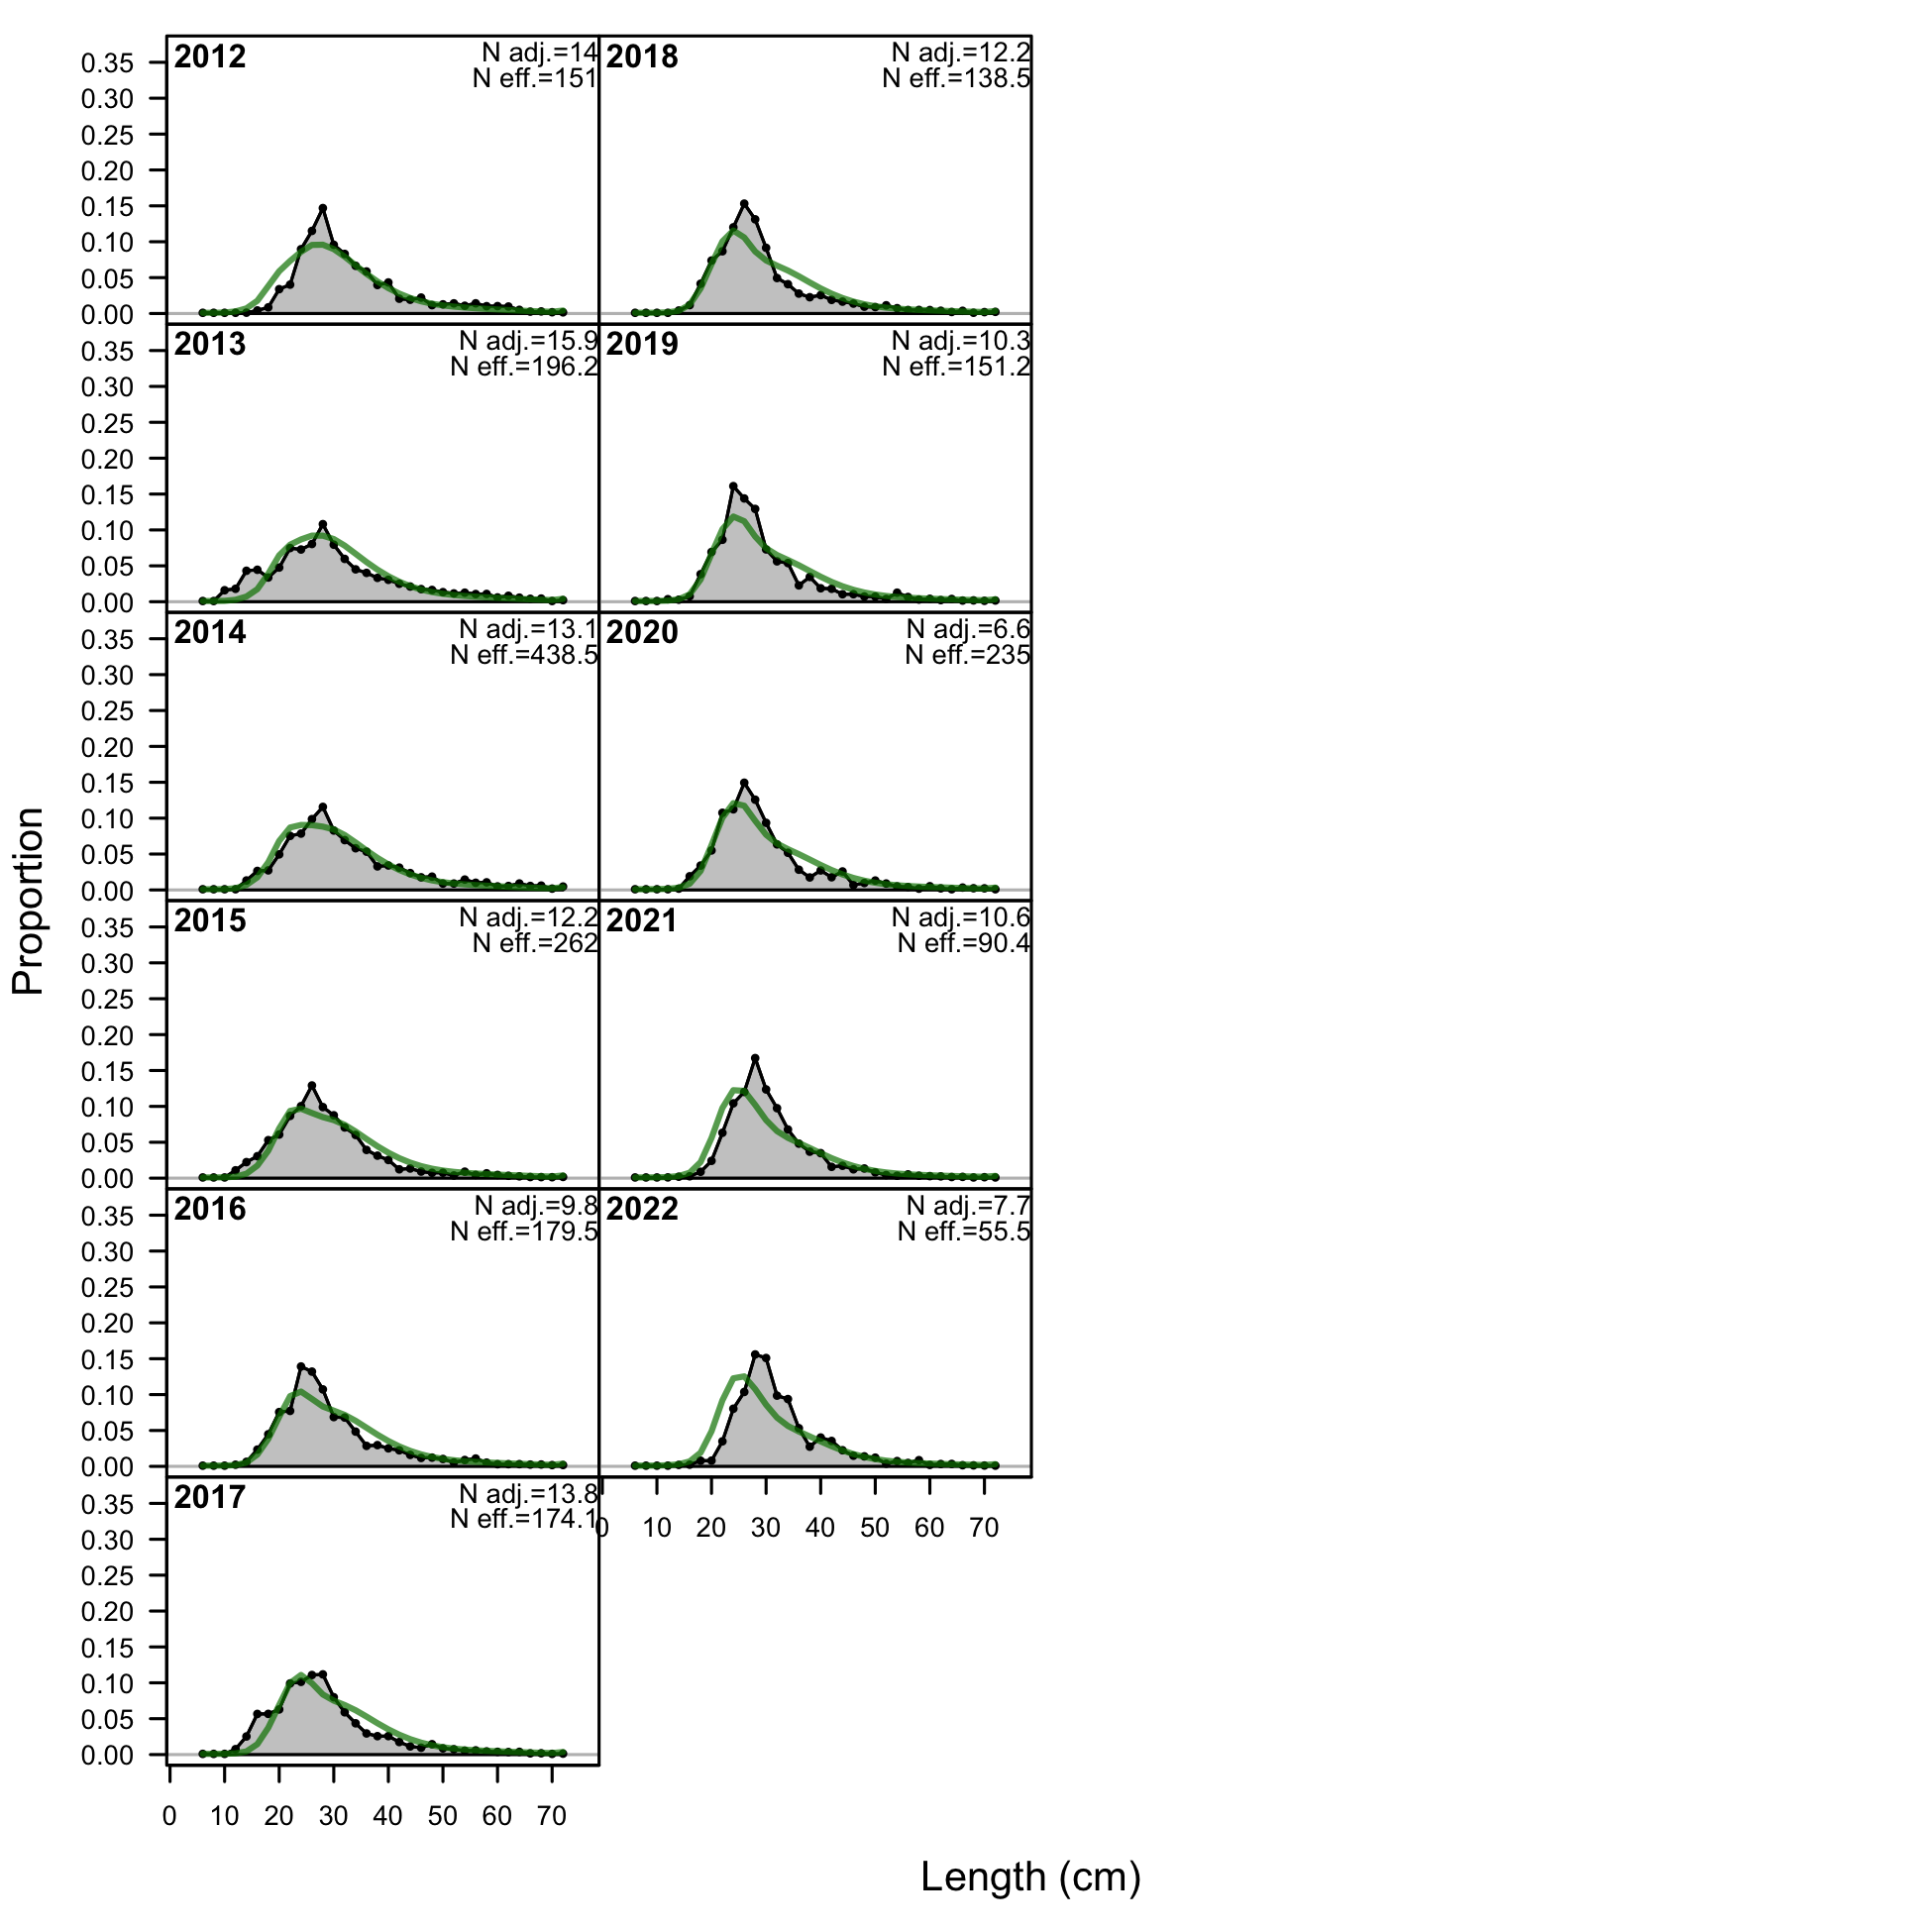
\includegraphics[width=1\textwidth,height=1\textheight]{C:/GitHub/Official_shortspine_thornyhead_2023/doc/FinalFigs/Base/comp_lenfit_flt1mkt2_page2.png}
\caption{Annual length comps and model fit for North trawl retained catch. `N adj.' is the input sample size after data-weighting adjustment. N eff. is the calculated effective sample size used in the McAllister-Ianelli tuning method.\label{fig:ntrawl_comps_2}}
\end{figure}

\begin{figure}
\centering
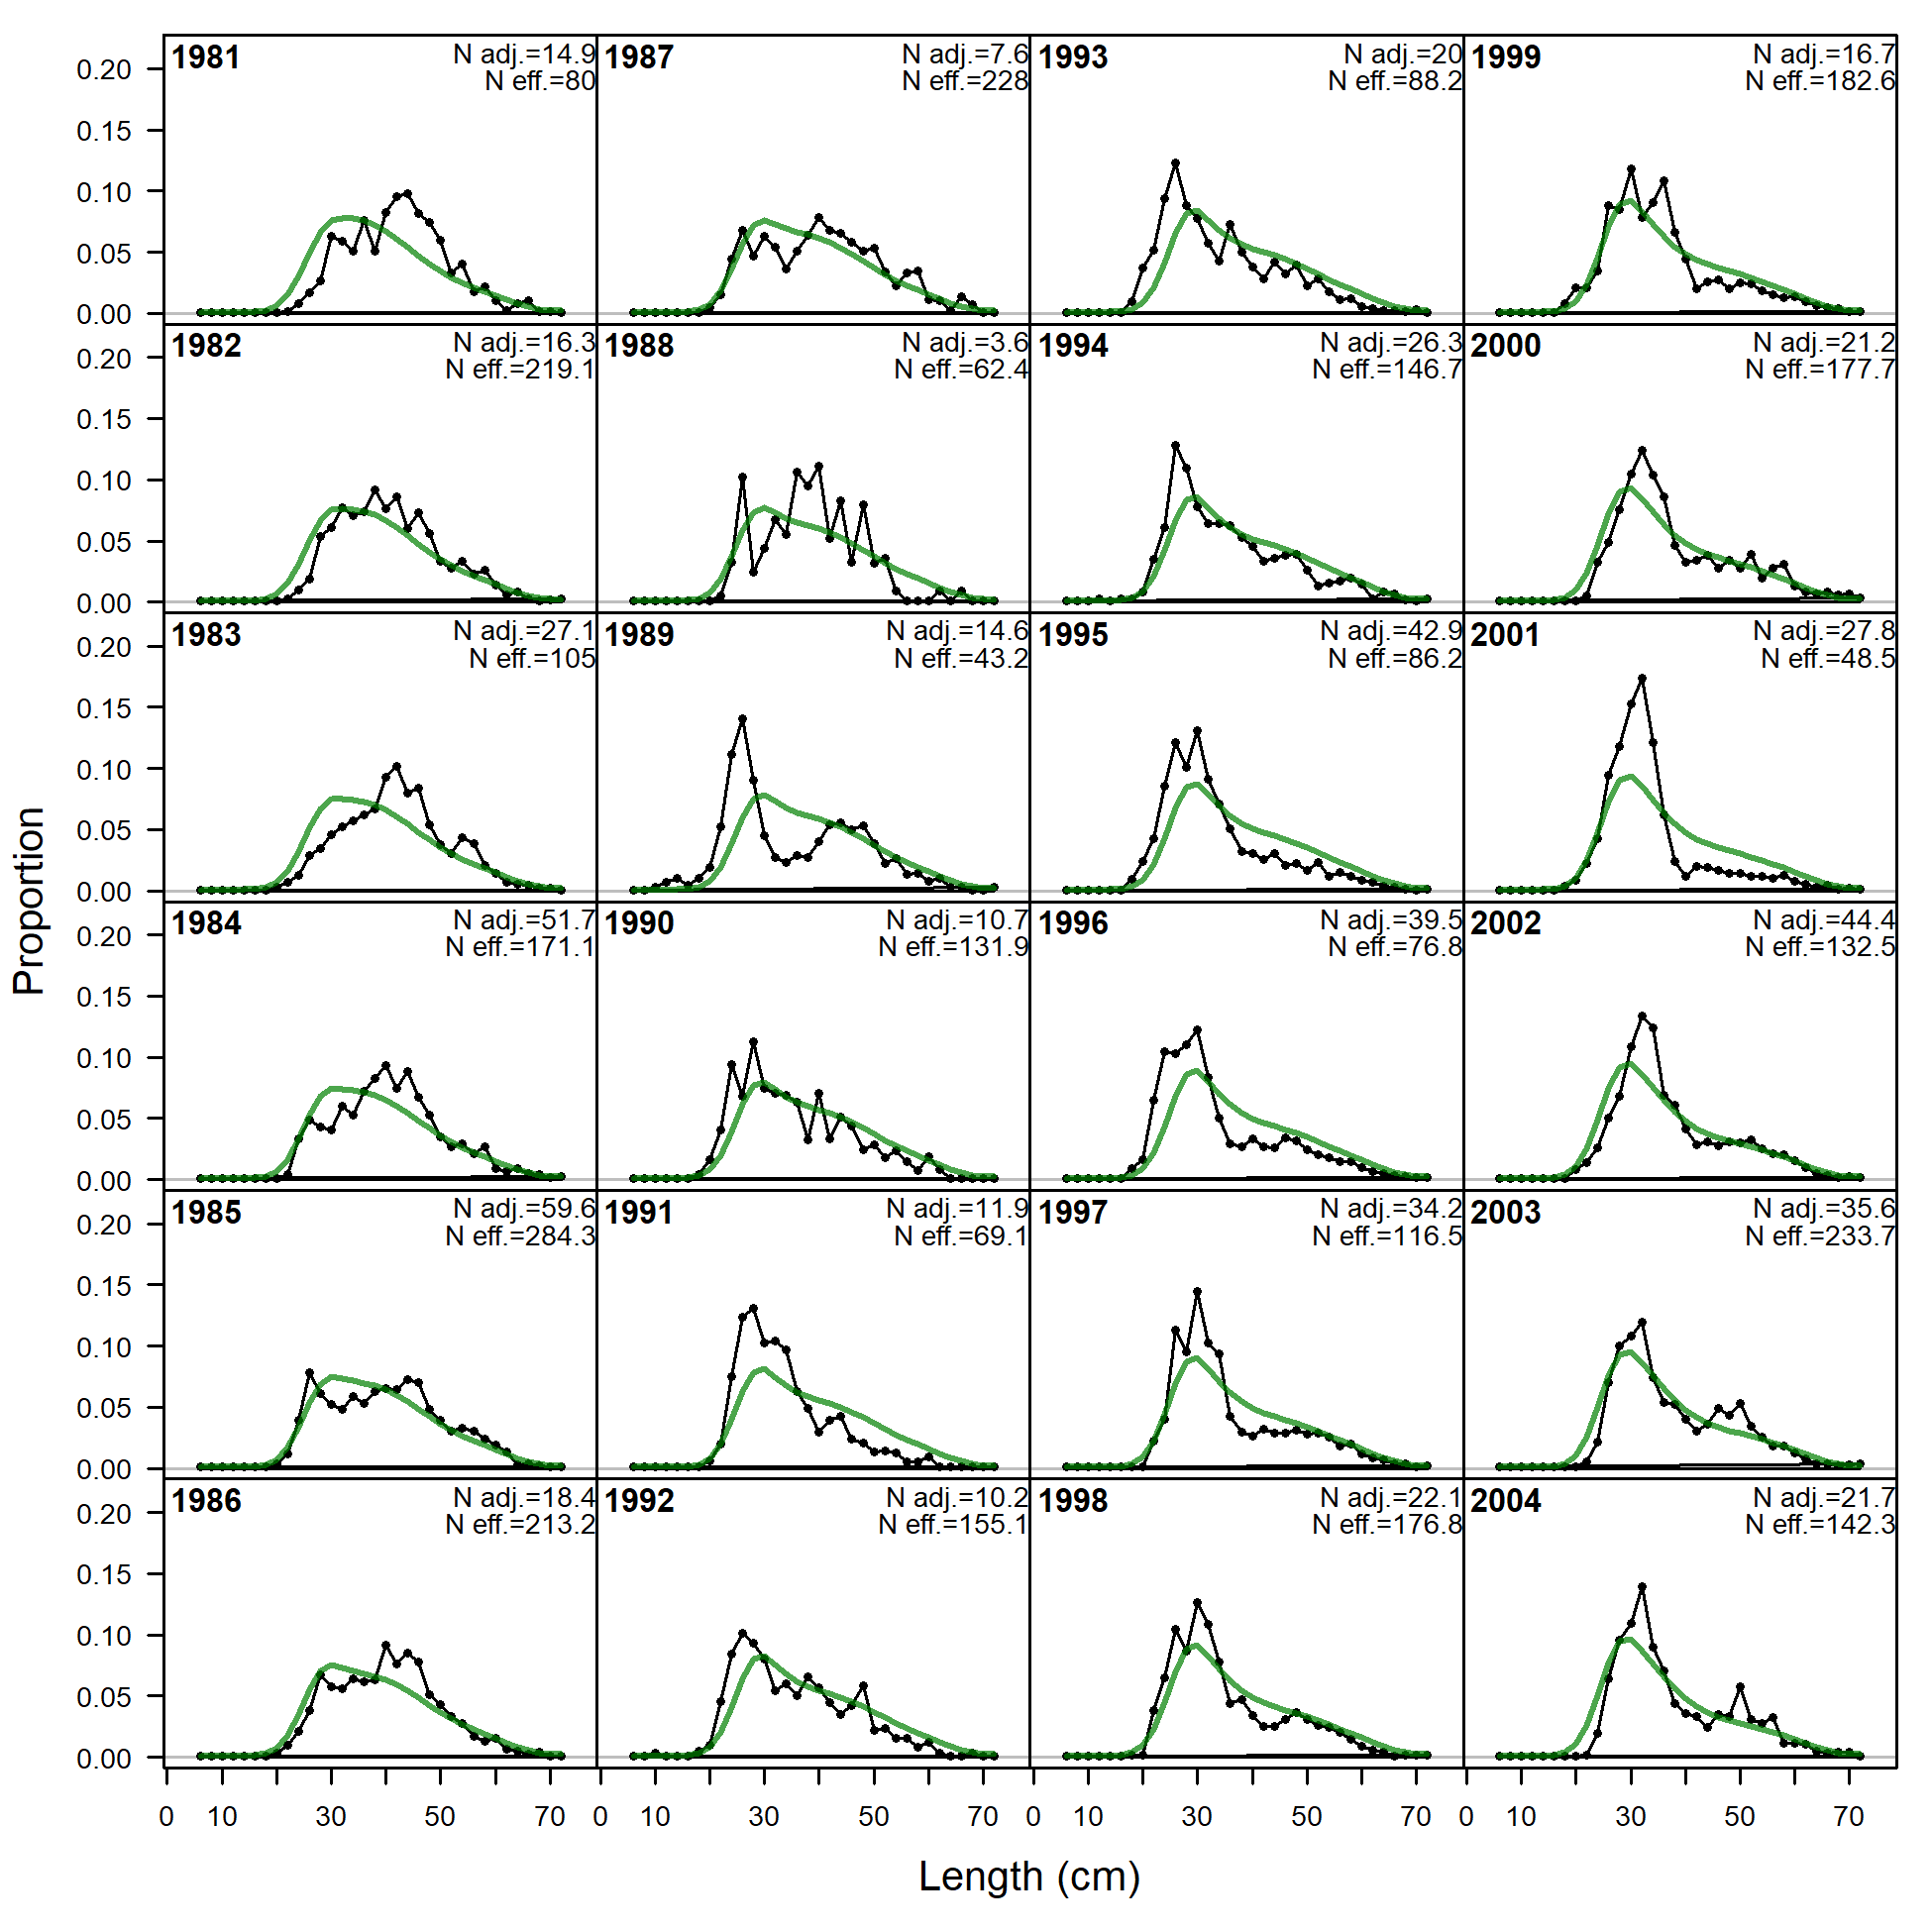
\includegraphics[width=1\textwidth,height=1\textheight]{C:/GitHub/Official_shortspine_thornyhead_2023/doc/FinalFigs/Base/comp_lenfit_flt2mkt2_page1.png}
\caption{Annual length comps and model fit for South trawl retained catch. `N adj.' is the input sample size after data-weighting adjustment. N eff. is the calculated effective sample size used in the McAllister-Ianelli tuning method.\label{fig:strawl_comps_1}}
\end{figure}

\begin{figure}
\centering
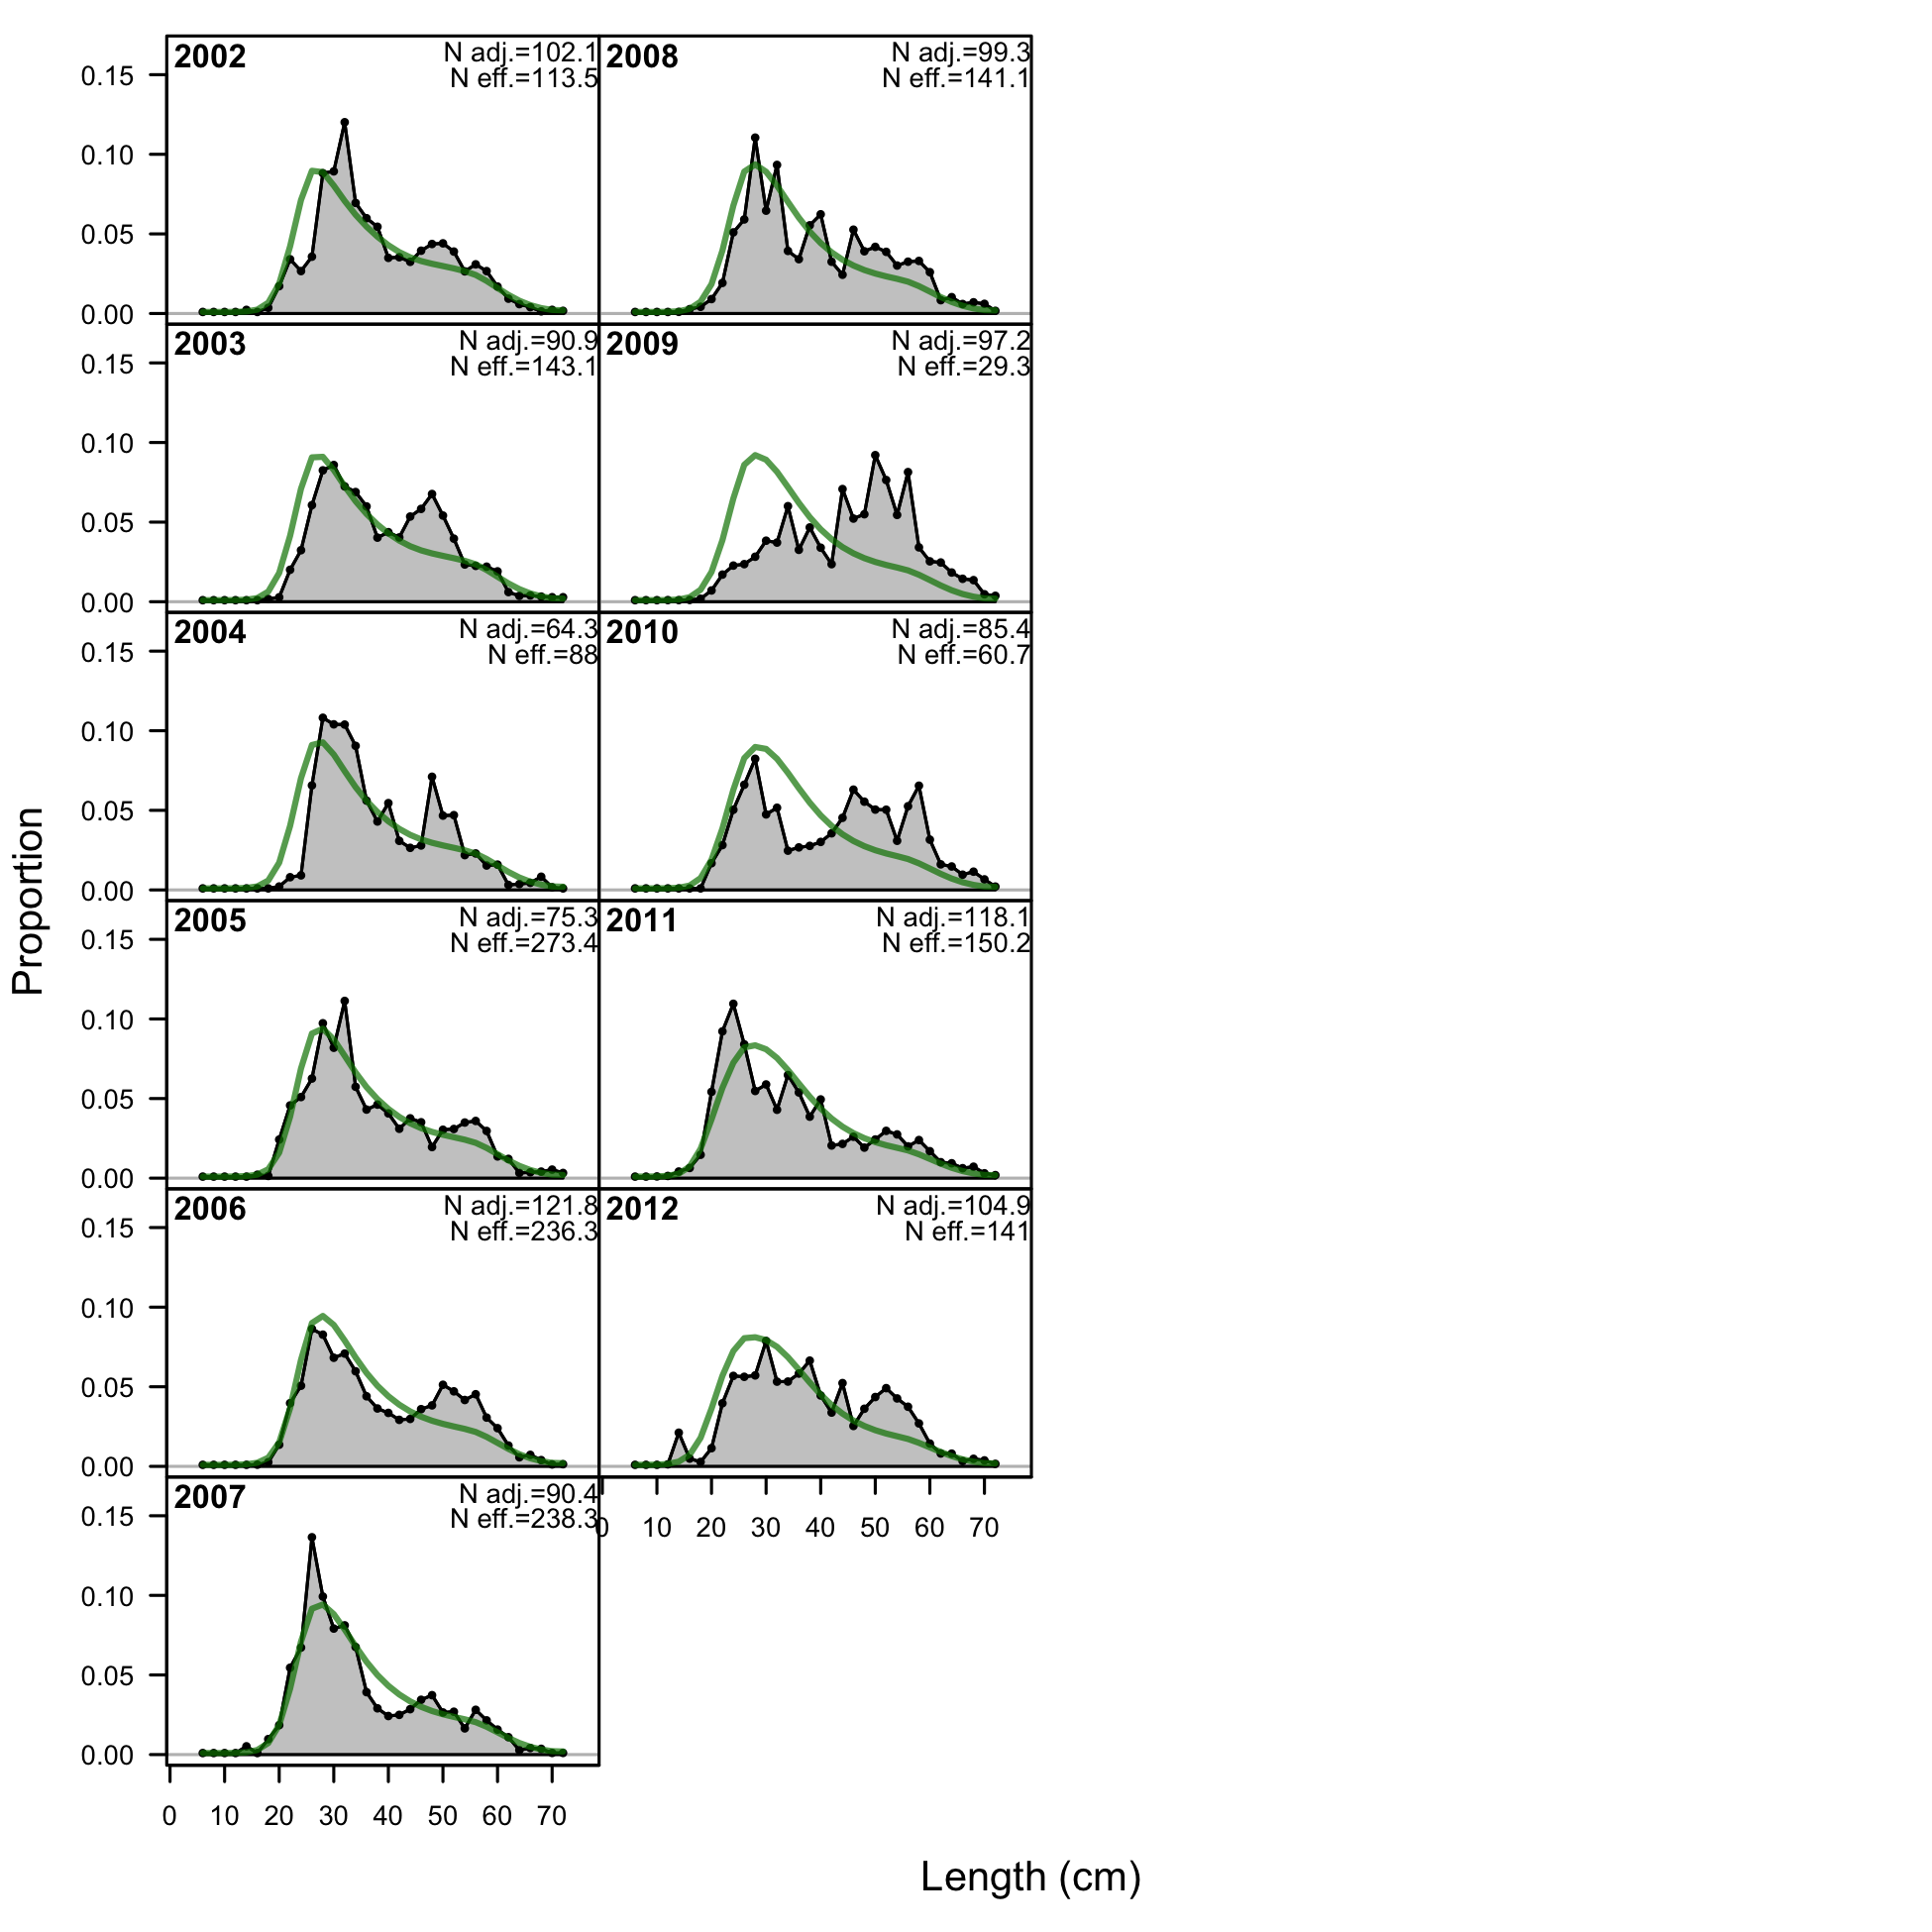
\includegraphics[width=1\textwidth,height=1\textheight]{C:/GitHub/Official_shortspine_thornyhead_2023/doc/FinalFigs/Base/comp_lenfit_flt2mkt2_page2.png}
\caption{Annual length comps and model fit for South trawl retained catch. `N adj.' is the input sample size after data-weighting adjustment. N eff. is the calculated effective sample size used in the McAllister-Ianelli tuning method.\label{fig:strawl_comps_2}}
\end{figure}

\begin{figure}
\centering
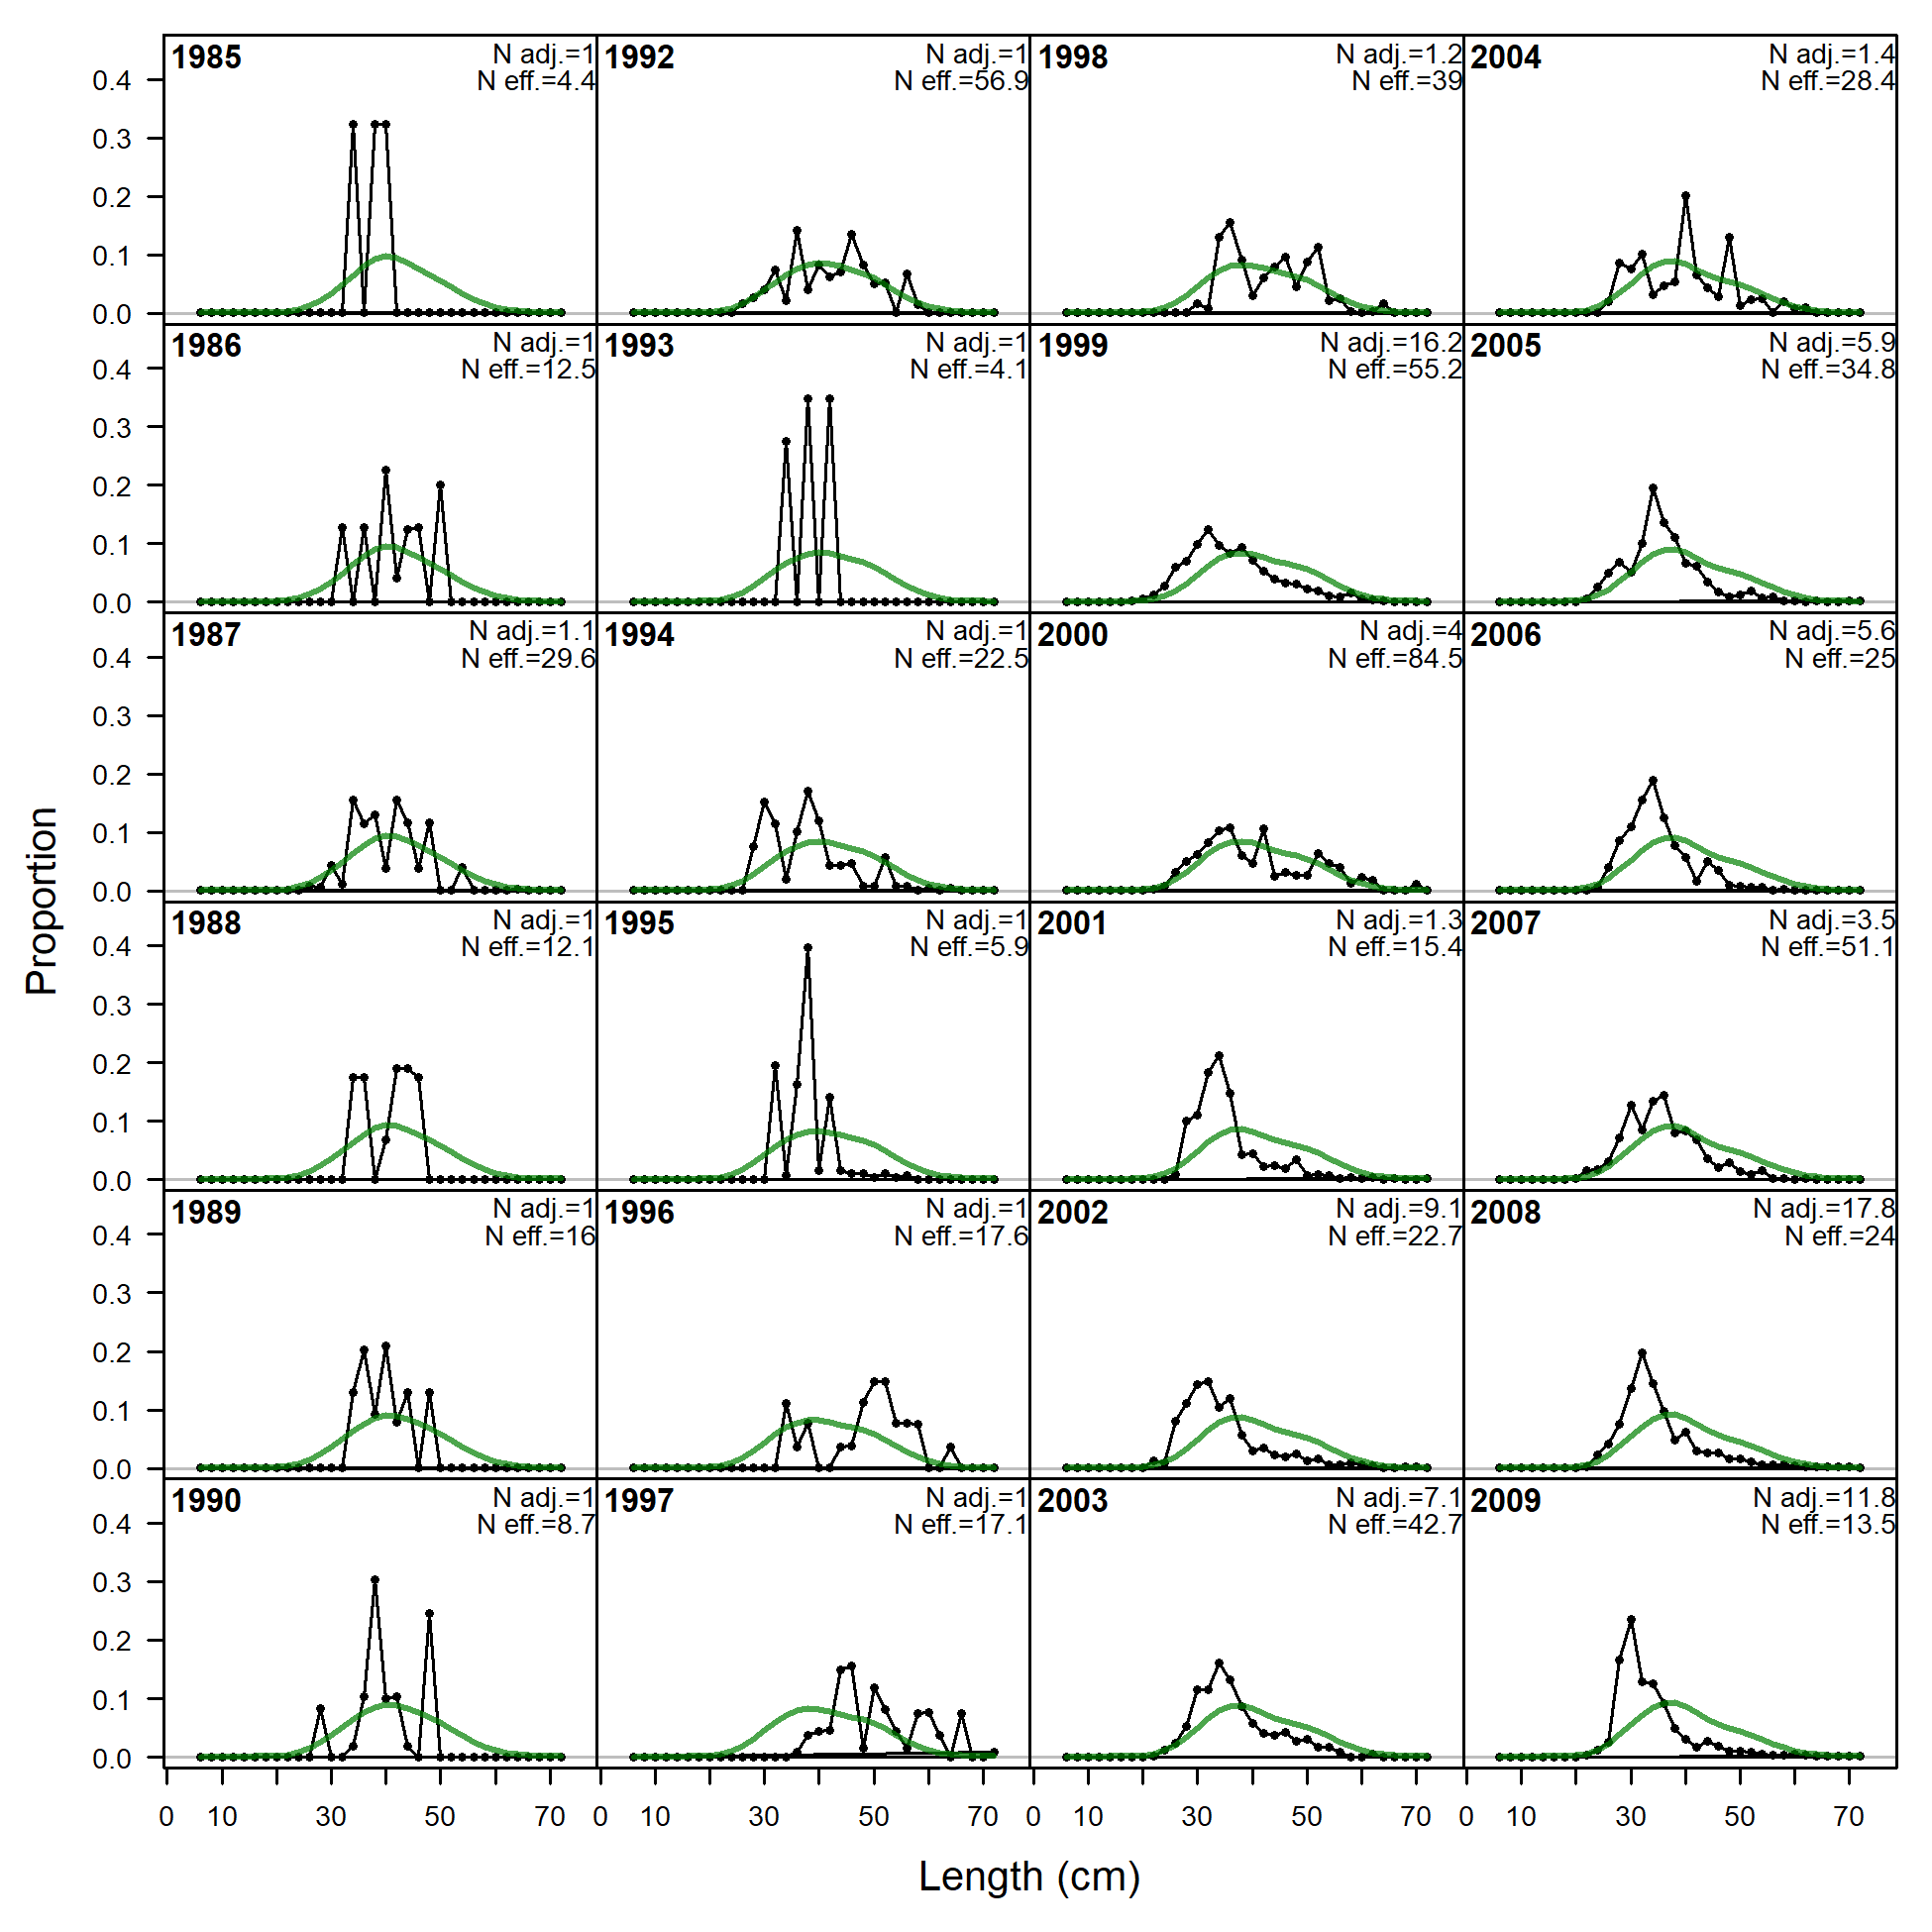
\includegraphics[width=1\textwidth,height=1\textheight]{C:/GitHub/Official_shortspine_thornyhead_2023/doc/FinalFigs/Base/comp_lenfit_flt3mkt2_page1.png}
\caption{Annual length comps and model fit for Non-trawl retained catch. `N adj.' is the input sample size after data-weighting adjustment. N eff. is the calculated effective sample size used in the McAllister-Ianelli tuning method.\label{fig:nontrawl_comps_1}}
\end{figure}

\begin{figure}
\centering
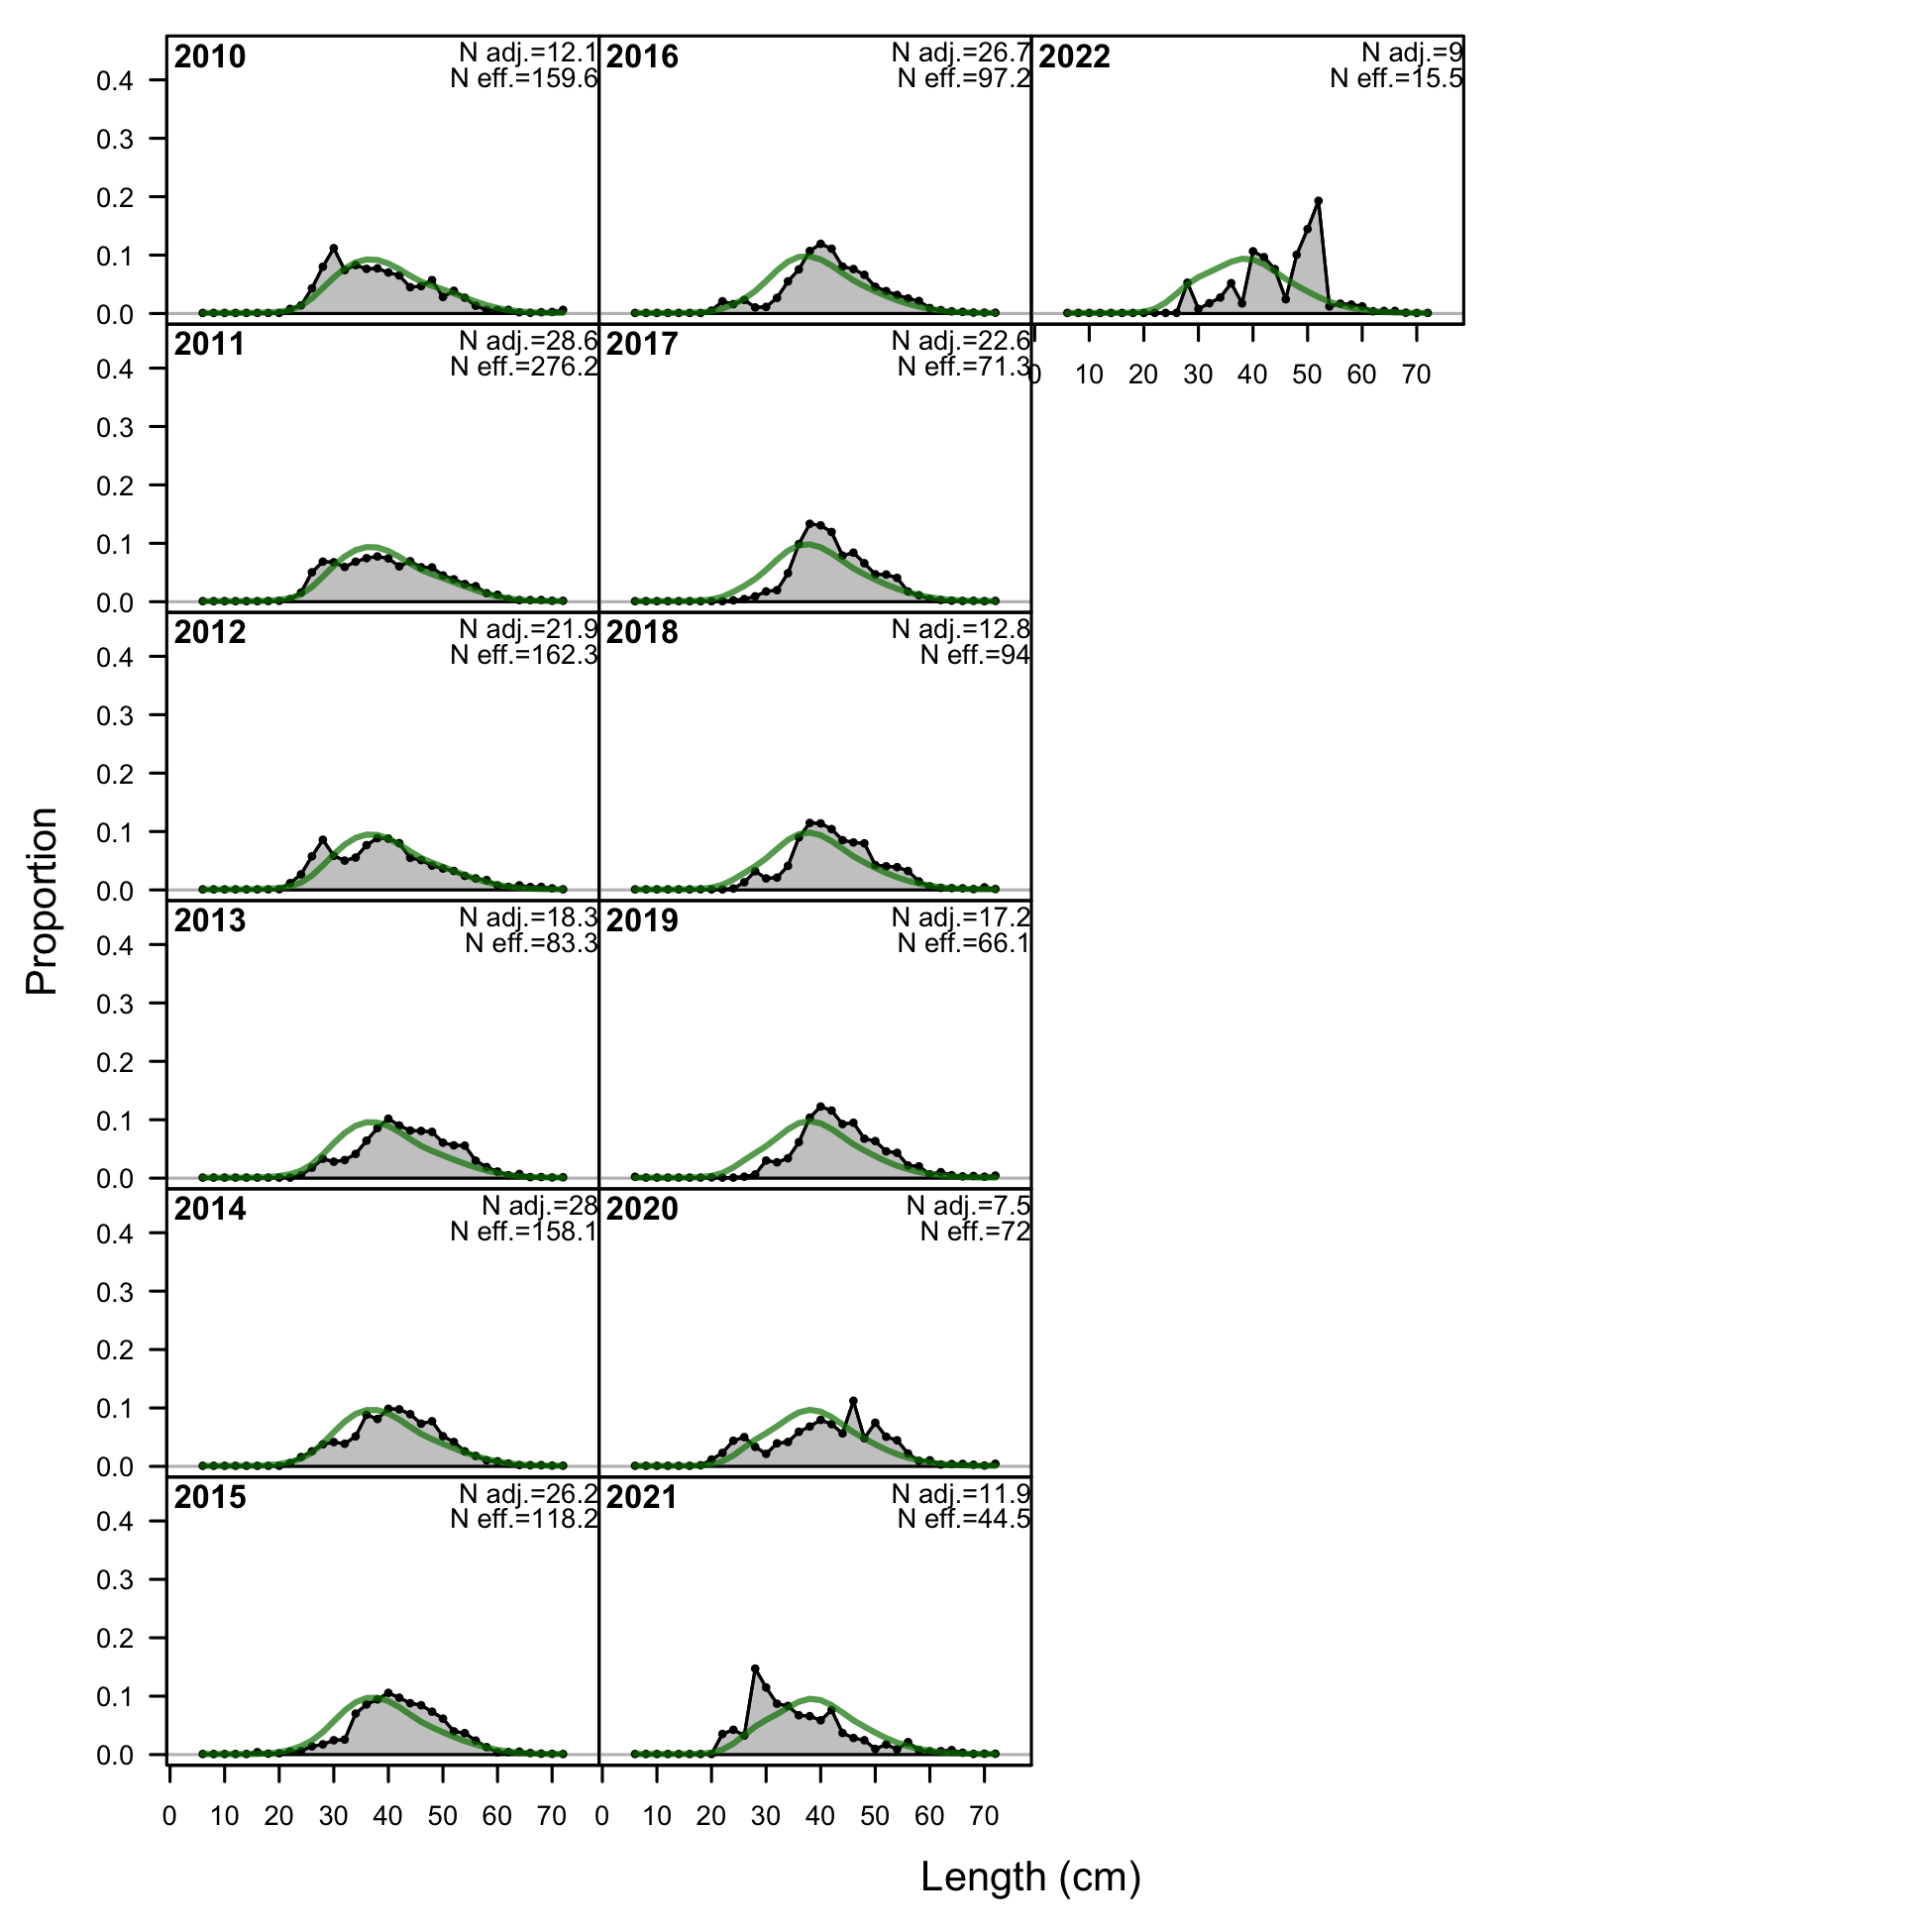
\includegraphics[width=1\textwidth,height=1\textheight]{C:/GitHub/Official_shortspine_thornyhead_2023/doc/FinalFigs/Base/comp_lenfit_flt3mkt2_page2.png}
\caption{Annual length comps and model fit for Non-trawl retained catch. `N adj.' is the input sample size after data-weighting adjustment. N eff. is the calculated effective sample size used in the McAllister-Ianelli tuning method.\label{fig:nontrawl_comps_2}}
\end{figure}

\begin{figure}
\centering
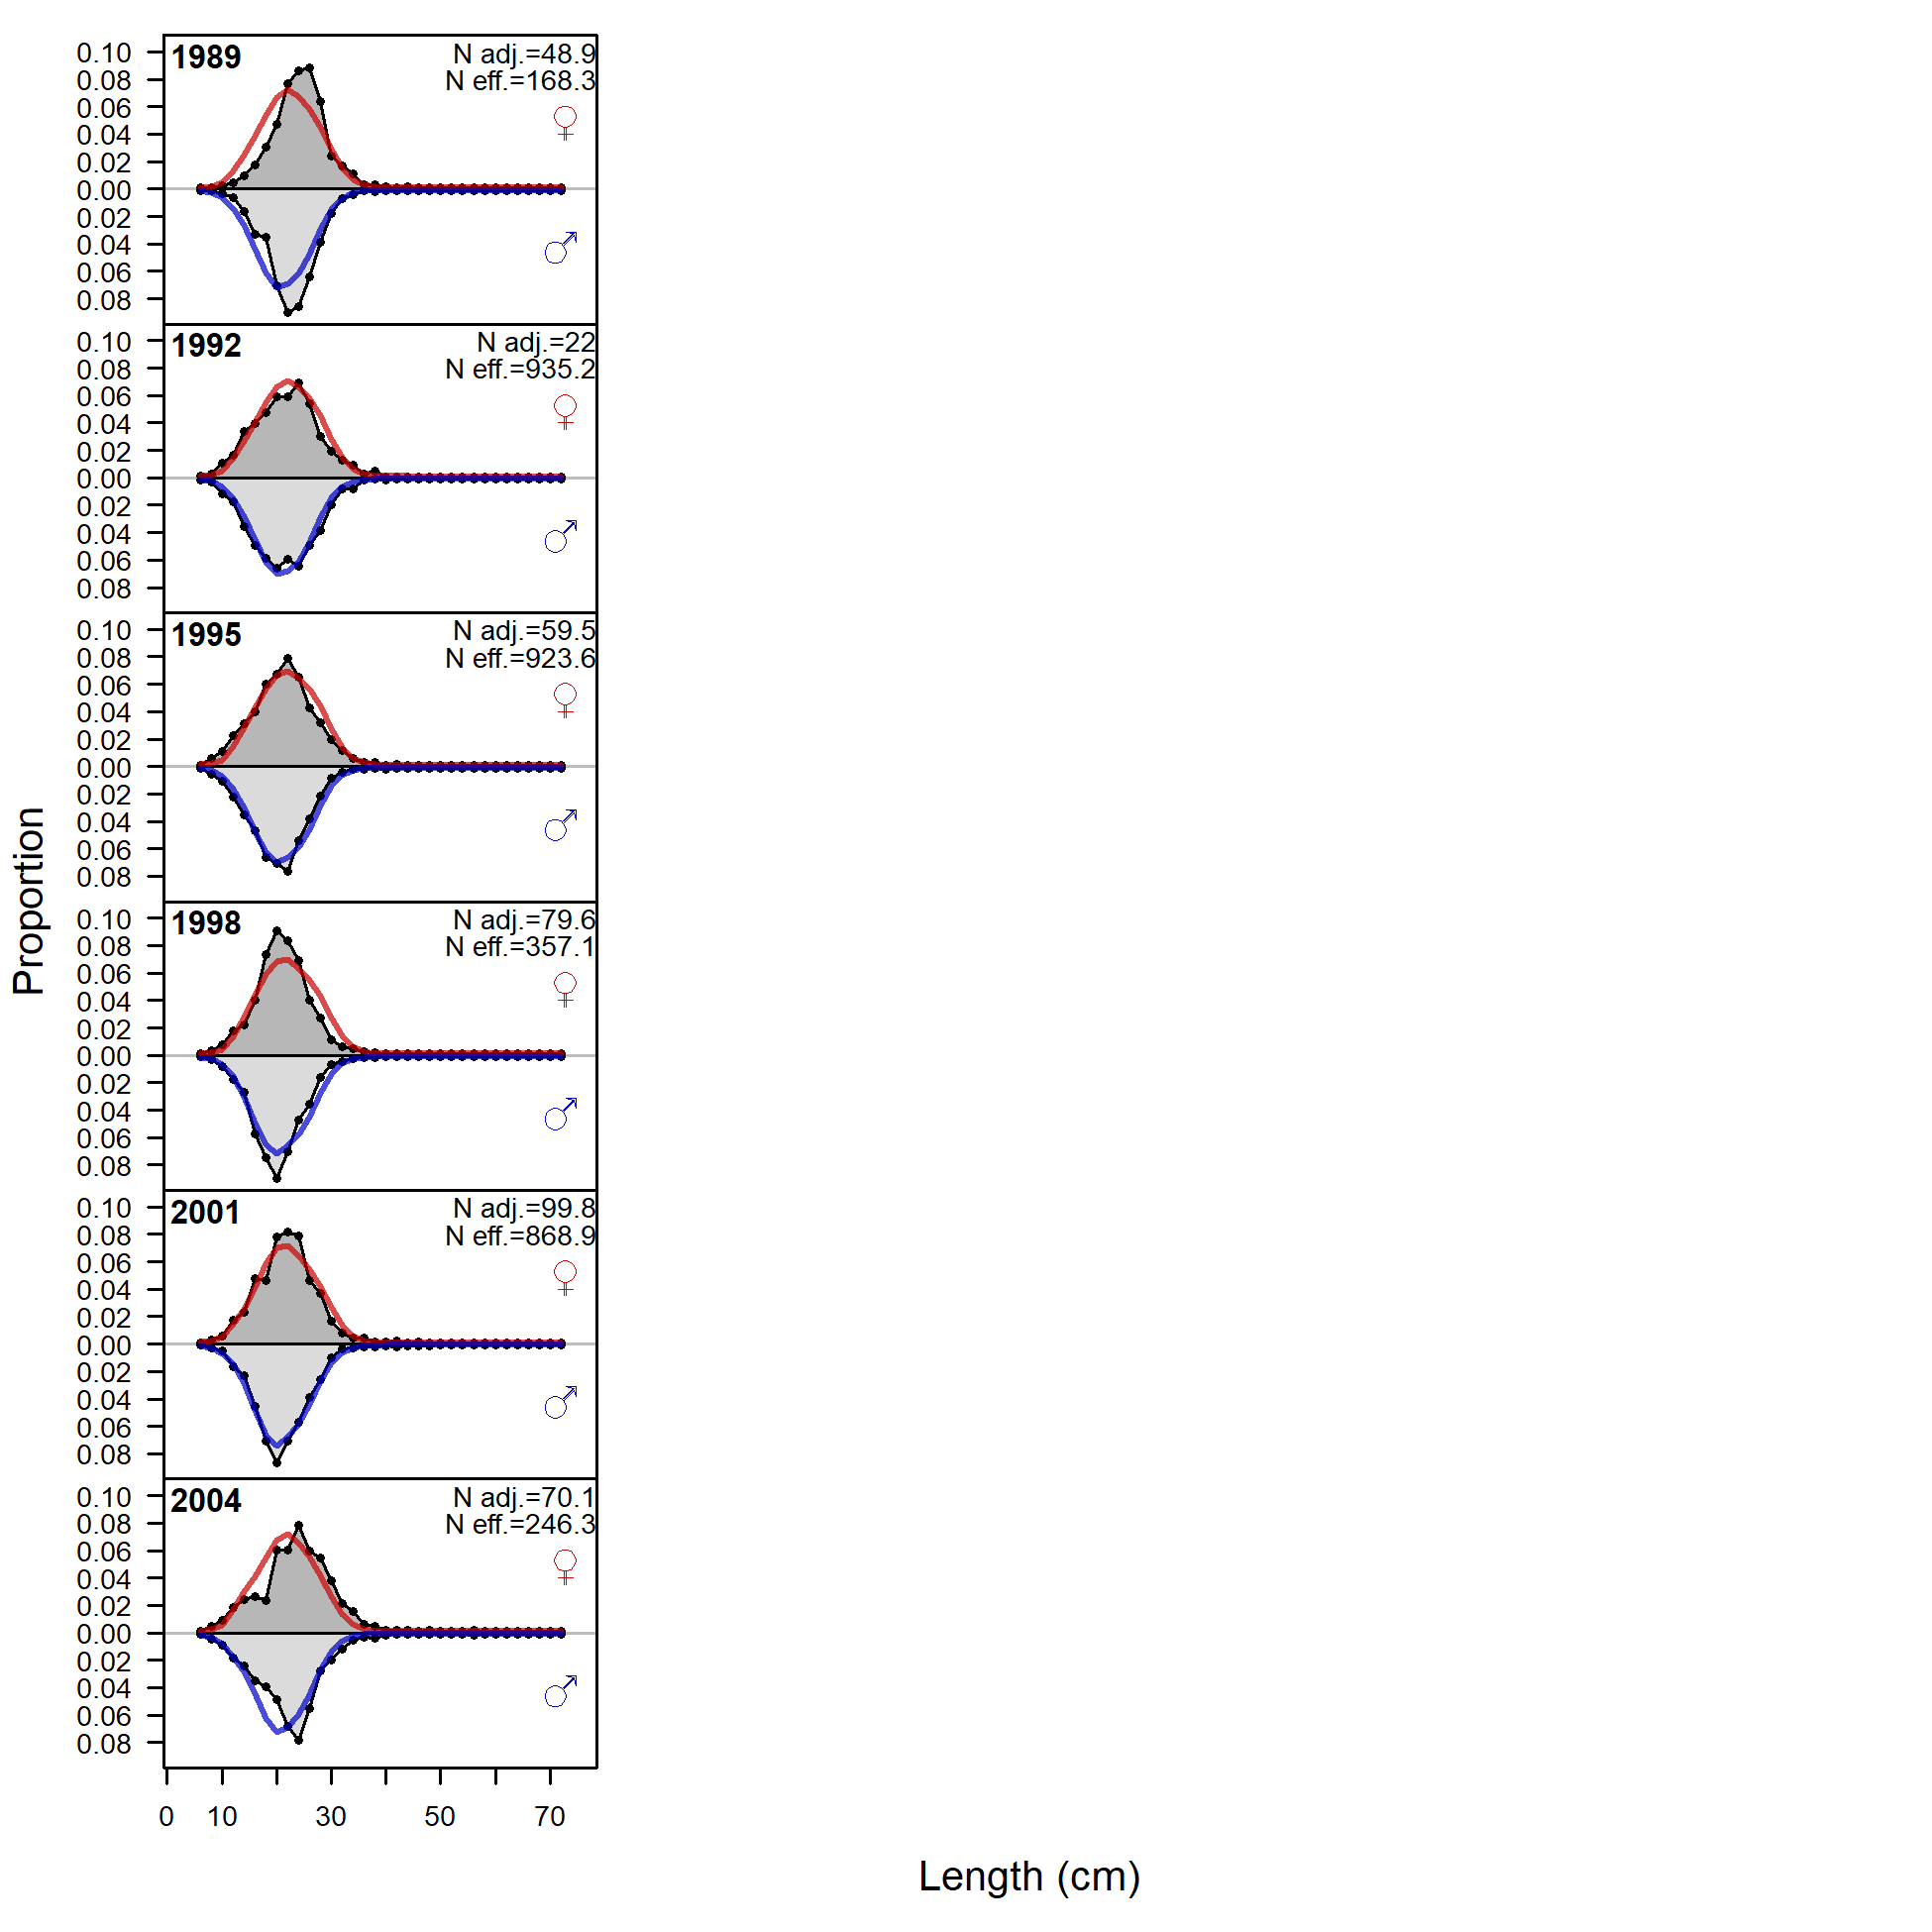
\includegraphics[width=1\textwidth,height=1\textheight]{C:/GitHub/Official_shortspine_thornyhead_2023/doc/FinalFigs/Base/comp_lenfit_flt4mkt0.png}
\caption{Length comps, whole catch, for the early-Triennial Survey (1980-1992). `N adj.' is the input sample size after data-weighting adjustment. N eff. is the calculated effective sample size used in the McAllister-Ianelli tuning method.\label{fig:fits_etri}}
\end{figure}

\begin{figure}
\centering
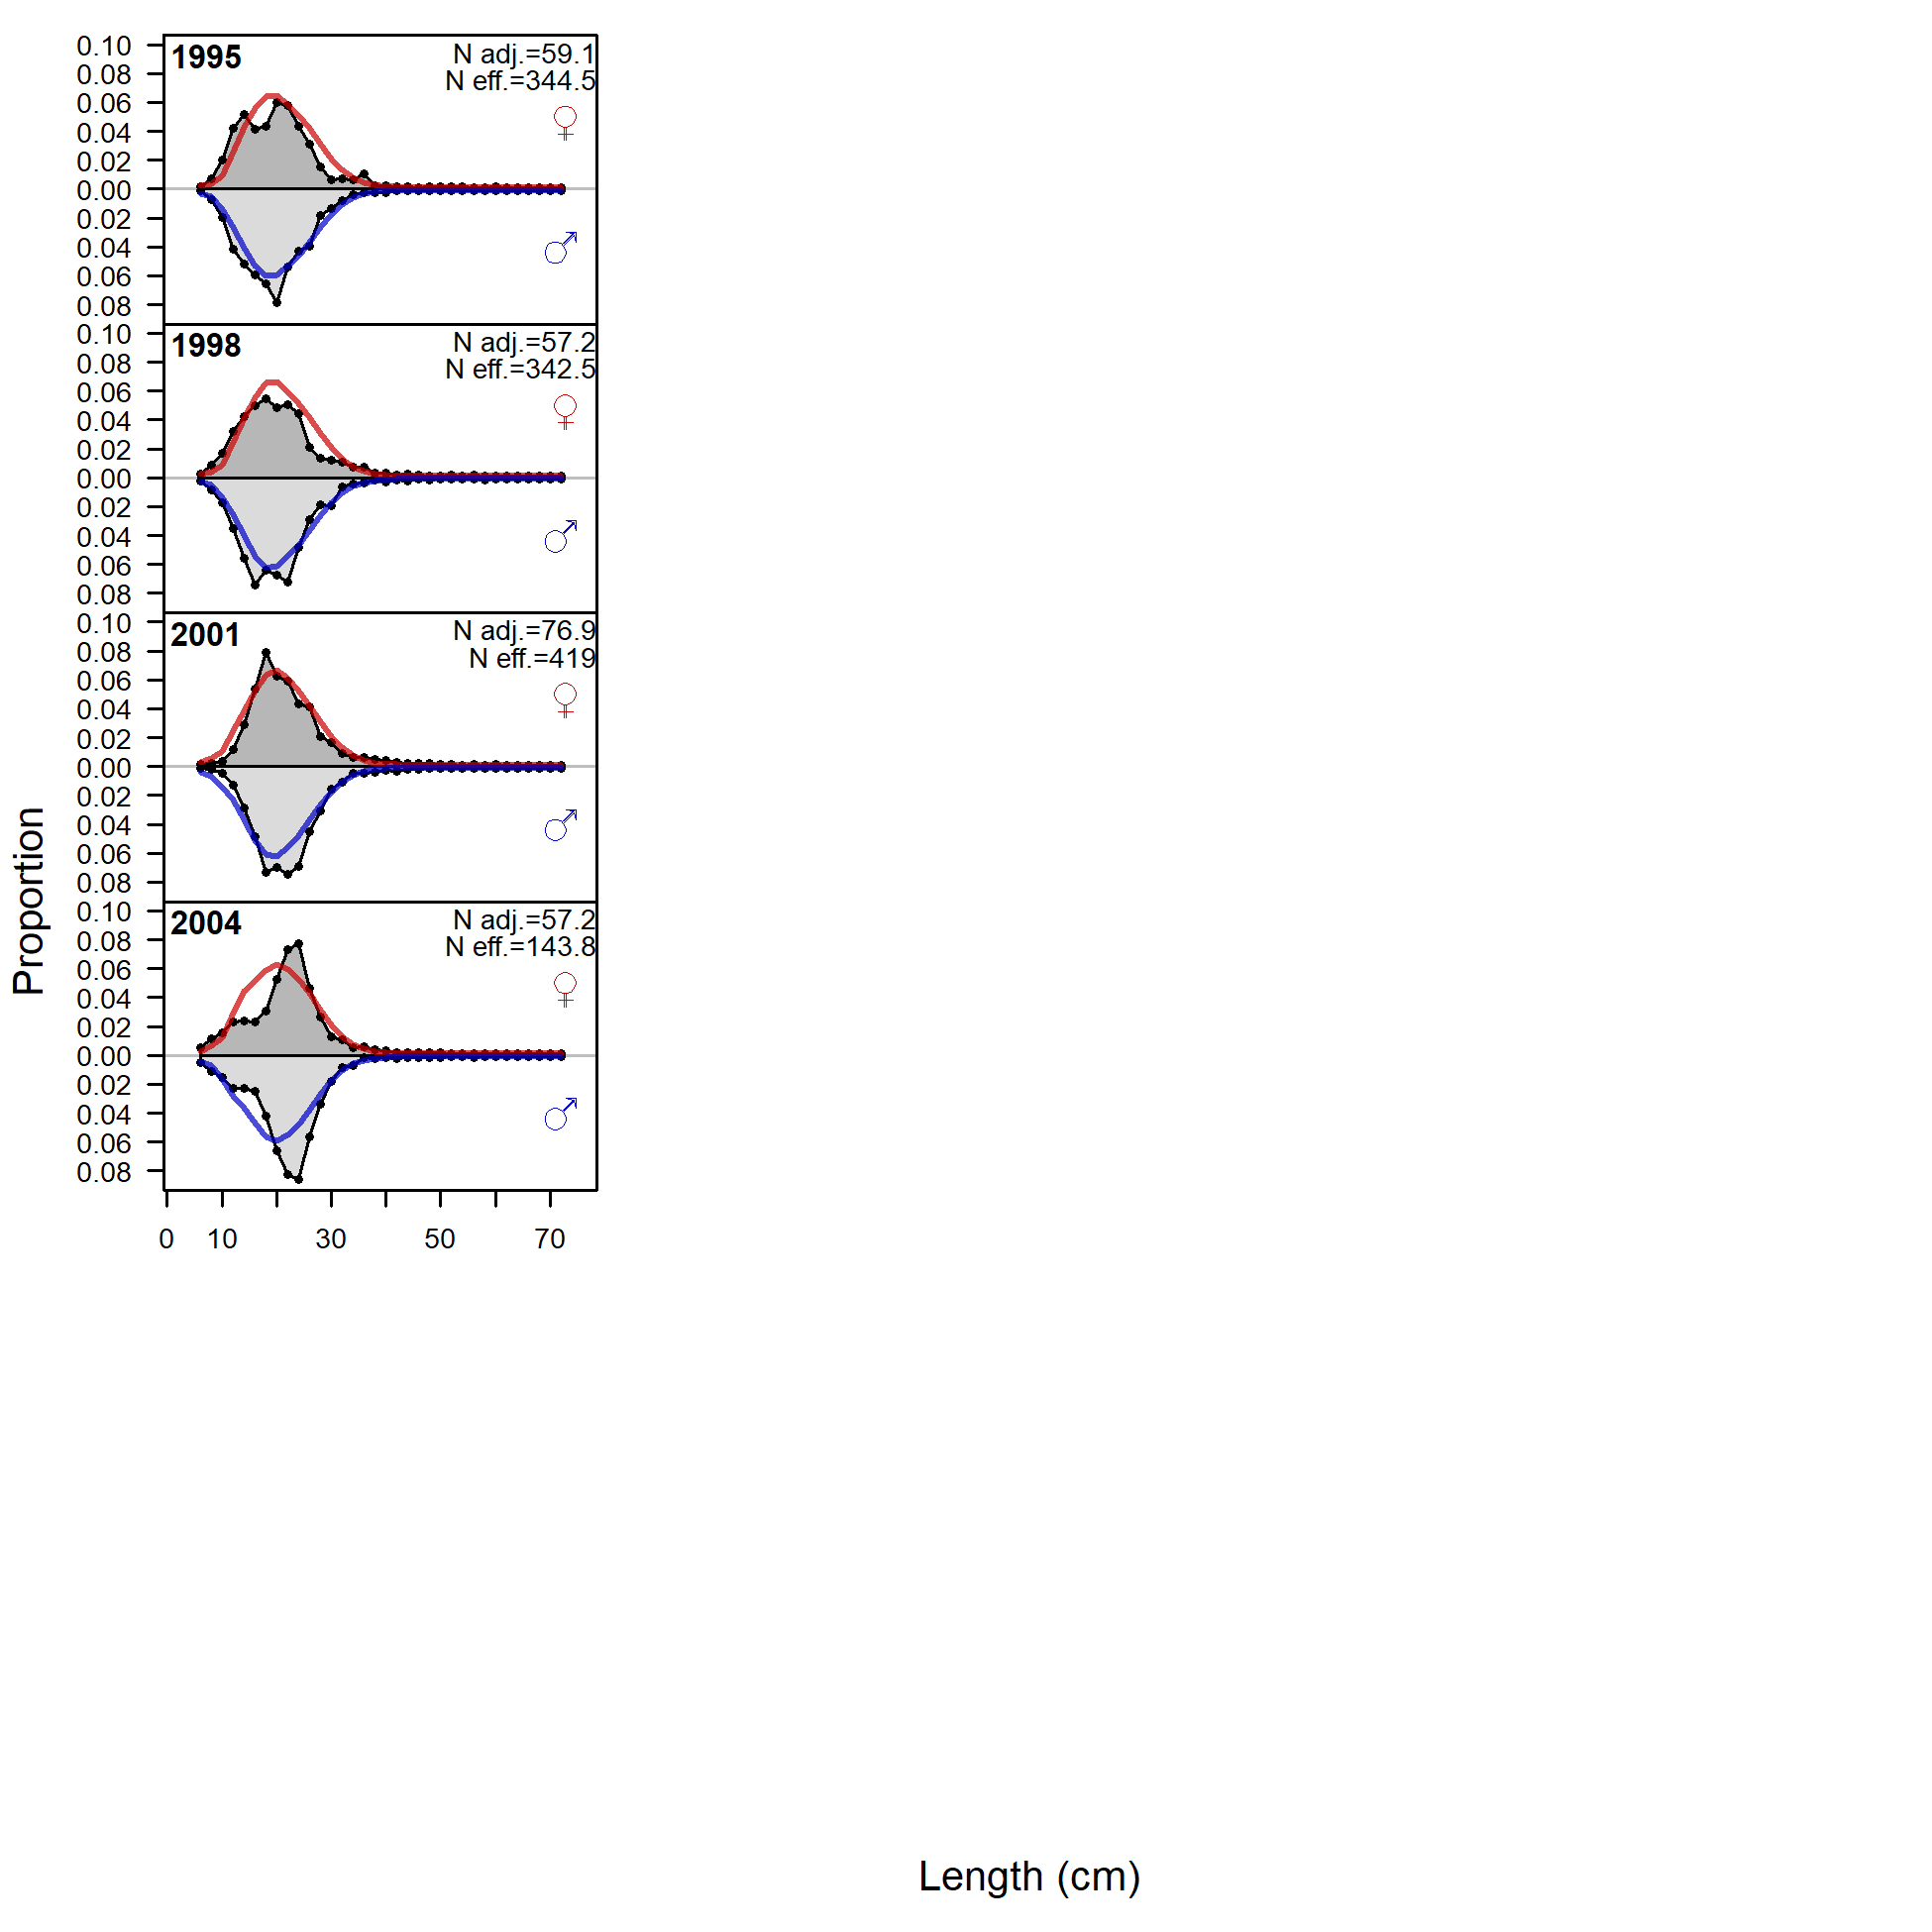
\includegraphics[width=1\textwidth,height=1\textheight]{C:/GitHub/Official_shortspine_thornyhead_2023/doc/FinalFigs/Base/comp_lenfit_flt5mkt0.png}
\caption{Length comps, whole catch, for the late-Triennial Survey (1995-2004). `N adj.' is the input sample size after data-weighting adjustment. N eff. is the calculated effective sample size used in the McAllister-Ianelli tuning method.\label{fig:fits_ltri}}
\end{figure}

\begin{figure}
\centering
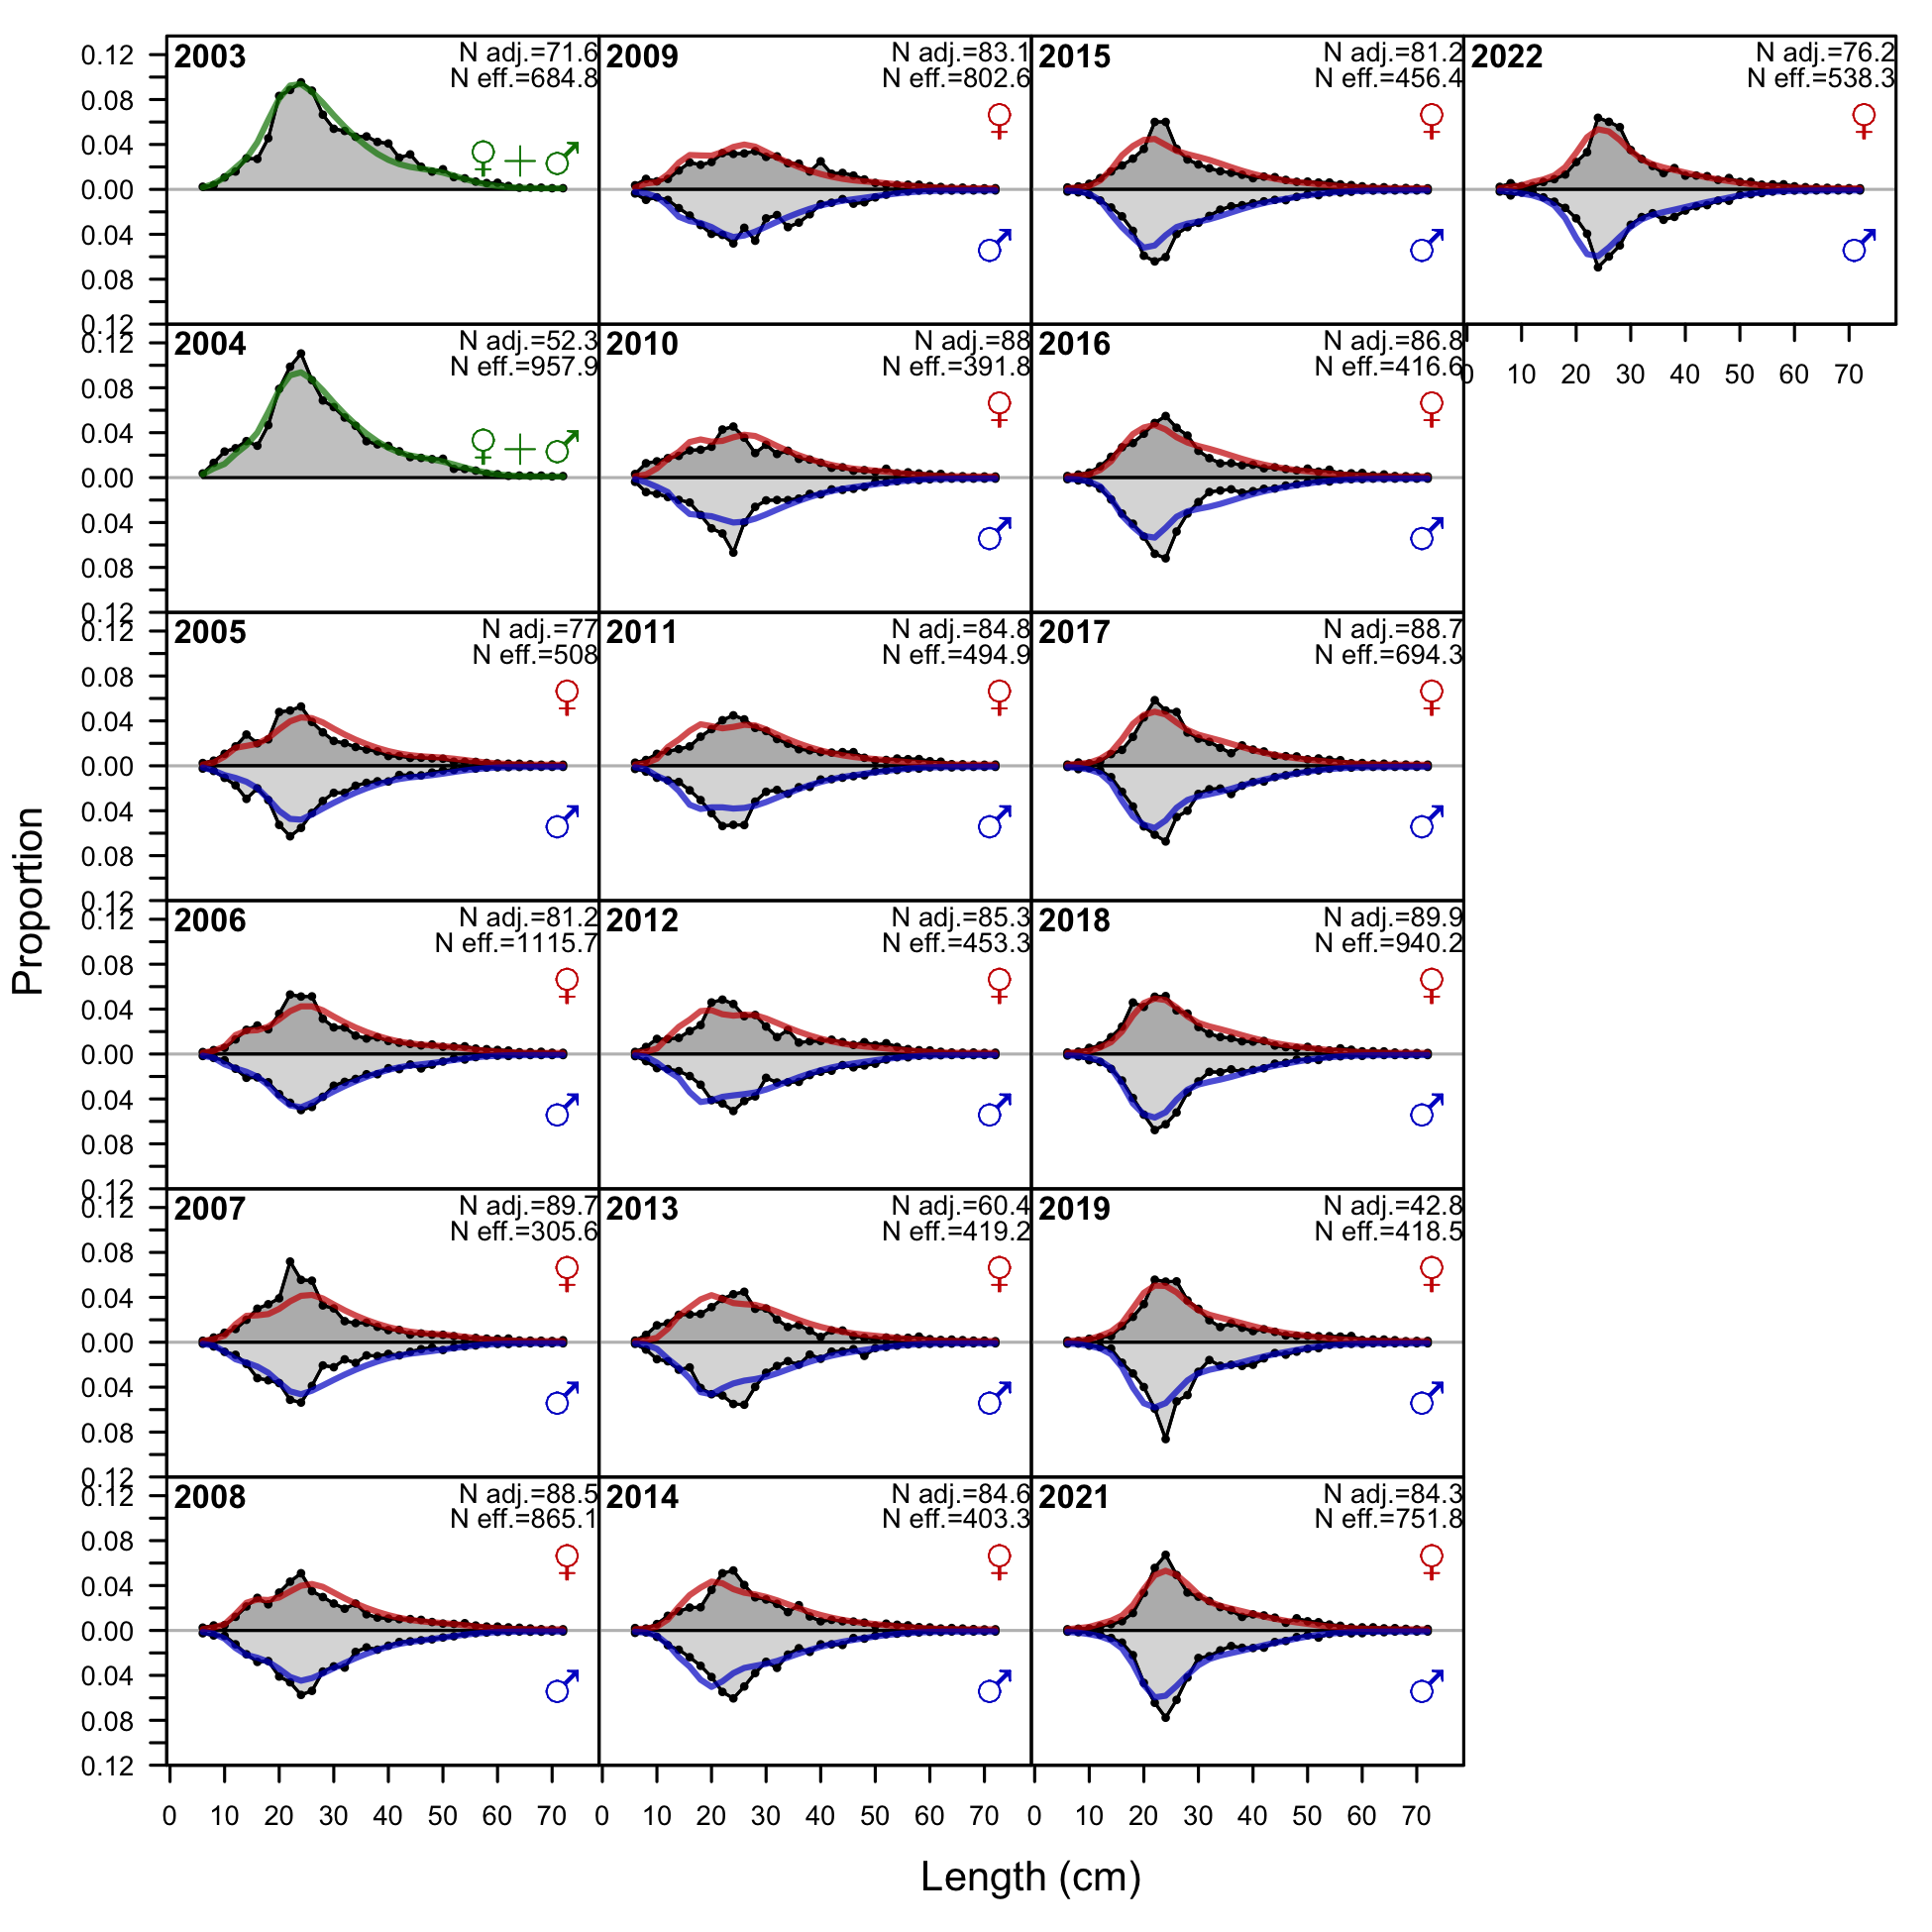
\includegraphics[width=1\textwidth,height=1\textheight]{C:/GitHub/Official_shortspine_thornyhead_2023/doc/FinalFigs/Base/comp_lenfit_flt6mkt0.png}
\caption{Length comps, whole catch, for the WCGBTS. `N adj.' is the input sample size after data-weighting adjustment. N eff. is the calculated effective sample size used in the McAllister-Ianelli tuning method.\label{fig:fits_wcgbts}}
\end{figure}

\begin{figure}
\centering
\includegraphics[width=1\textwidth,height=1\textheight]{C:/GitHub/Official_shortspine_thornyhead_2023/doc/FinalFigs/Base/comp_lenfit__page1_multi-fleet_comparison.png}
\caption{Pearson residuals, whole catch, for the three fisheries fleets. Closed bubbles are positive residuals (observed \textgreater{} expected) and open bubbles are negative residuals (observed \textless{} expected).\label{fig:resids_fisheries}}
\end{figure}

\begin{figure}
\centering
\includegraphics[width=1\textwidth,height=1\textheight]{C:/GitHub/Official_shortspine_thornyhead_2023/doc/FinalFigs/Base/comp_lenfit__page2_multi-fleet_comparison.png}
\caption{Pearson residuals, whole catch, for the three scientific surveys. Closed bubbles are positive residuals (observed \textgreater{} expected) and open bubbles are negative residuals (observed \textless{} expected). Red bubbles are female, blue bubbles are male, and grey bubble are unsexed.\label{fig:resids_survey}}
\end{figure}

\begin{figure}
\centering
\includegraphics[width=1\textwidth,height=1\textheight]{C:/GitHub/Official_shortspine_thornyhead_2023/doc/FinalFigs/Base/bodywt_fit_fltTrawl_N.png}
\caption{Mean individual body weight (kg) in discard for the North trawl fleet.\label{fig:weightNorthTrl}}
\end{figure}

\begin{figure}
\centering
\includegraphics[width=1\textwidth,height=1\textheight]{C:/GitHub/Official_shortspine_thornyhead_2023/doc/FinalFigs/Base/bodywt_fit_fltTrawl_S.png}
\caption{Mean individual body weight (kg) in discard for the South trawl fleet.\label{fig:weightSouthTrl}}
\end{figure}

\begin{figure}
\centering
\includegraphics[width=1\textwidth,height=1\textheight]{C:/GitHub/Official_shortspine_thornyhead_2023/doc/FinalFigs/Base/bodywt_fit_fltNon-trawl.png}
\caption{Mean individual body weight (kg) in discard for the Non-trawl fleet.\label{fig:weightNonTrl}}
\end{figure}

\begin{figure}
\centering
\includegraphics[width=1\textwidth,height=1\textheight]{C:/GitHub/Official_shortspine_thornyhead_2023/doc/FinalFigs/Base/ts7_Spawning_output_with_95_asymptotic_intervals_intervals.png}
\caption{Spawning output (eggs) with \textasciitilde95\% asymptotic intervals.\label{fig:spawnout}}
\end{figure}

\begin{figure}
\centering
\includegraphics[width=1\textwidth,height=1\textheight]{C:/GitHub/Official_shortspine_thornyhead_2023/doc/FinalFigs/Base/ts9_Relative_spawning_output_intervals.png}
\caption{Relative spawning output: \(B/B_0\) with \textasciitilde95\% asymptotic intervals.\label{fig:relspawnout}}
\end{figure}

\begin{figure}
\centering
\includegraphics[width=1\textwidth,height=1\textheight]{C:/GitHub/Official_shortspine_thornyhead_2023/doc/FinalFigs/Base/ts_summaryF.png}
\caption{Summary fishing mortality rate (total landings / summary biomass).\label{fig:summary_f}}
\end{figure}

\begin{figure}
\centering
\includegraphics[width=1\textwidth,height=1\textheight]{C:/GitHub/Official_shortspine_thornyhead_2023/doc/FinalFigs/Base/SPR3_ratiointerval.png}
\caption{Estimated relative fishing intensity as a function of spawning potential ratio (SPR).\label{fig:spr_trajectory}}
\end{figure}

\begin{figure}
\centering
\includegraphics[width=1\textwidth,height=1\textheight]{C:/GitHub/Official_shortspine_thornyhead_2023/doc/FinalFigs/Base/SPR4_phase.png}
\caption{Phase plot of biomass ratio vs.~spawning potential ratio (SPR) ratio. Points represent the annual biomass ratio and SPR ratio. Lines through the final point show 95\% intervals based on the asymptotic uncertainty for each dimension, while the shaded ellipse is a 95\% region accoutninf for estimated correlation between the two quantities.\label{fig:phase_diagram}}
\end{figure}

\clearpage

\hypertarget{likelihood-profiles-retrospectives-and-sensitivity-analyses}{%
\subsection{Likelihood Profiles, Retrospectives, and Sensitivity Analyses}\label{likelihood-profiles-retrospectives-and-sensitivity-analyses}}

\begin{figure}
\centering
\includegraphics[width=1\textwidth,height=1\textheight]{C:/GitHub/Official_shortspine_thornyhead_2023/doc/FinalFigs/Profiles/piner_panel_SR_LN(R0).png}
\caption{Piner panel plot showing the impact of changing \(R_0\) on the overall (top), length composition (middle), and survy (bottom) likeihoods.\label{fig:R0_prof}}
\end{figure}

\begin{figure}
\centering
\includegraphics[width=1\textwidth,height=1\textheight]{C:/GitHub/Official_shortspine_thornyhead_2023/doc/FinalFigs/Profiles/SR_LN(R0)_trajectories_compare3_Bratio.png}
\caption{High to low values of \(R_0\) and impact on spawning output.\label{fig:R0_spawnout}}
\end{figure}

\begin{figure}
\centering
\includegraphics[width=1\textwidth,height=1\textheight]{C:/GitHub/Official_shortspine_thornyhead_2023/doc/FinalFigs/Profiles/piner_panel_SR_BH_steep.png}
\caption{Piner panel plot showing the impact of changing \(h\) on the overall (top), length composition (middle), and survy (bottom) likeihoods.\label{fig:h_piner_prof}}
\end{figure}

\begin{figure}
\centering
\includegraphics[width=1\textwidth,height=1\textheight]{C:/GitHub/Official_shortspine_thornyhead_2023/doc/FinalFigs/Profiles/SR_BH_steep_trajectories_compare3_Bratio.png}
\caption{High to low values of \(h\) and impact on relative spawning output.\label{fig:h_spawnout}}
\end{figure}

\begin{figure}
\centering
\includegraphics[width=1\textwidth,height=1\textheight]{C:/GitHub/Official_shortspine_thornyhead_2023/doc/FinalFigs/Profiles/piner_panel_NatM_break_1_Fem_GP_1.png}
\caption{Piner panel plot showing the impact of changing natural mortality (\(M\)) on the overall (top), length composition (middle), and survy (bottom) likeihoods.\label{fig:M_prof}}
\end{figure}

\begin{figure}
\centering
\includegraphics[width=1\textwidth,height=1\textheight]{C:/GitHub/Official_shortspine_thornyhead_2023/doc/FinalFigs/Profiles/NatM_break_1_Fem_GP_1_trajectories_compare1_spawnbio.png}
\caption{High to low values of \(M\) and impact on spawning output.\label{fig:M_spawnout}}
\end{figure}

\begin{figure}
\centering
\includegraphics[width=1\textwidth,height=1\textheight]{C:/GitHub/Official_shortspine_thornyhead_2023/doc/FinalFigs/Profiles/NatM_break_1_Fem_GP_1_trajectories_compare3_Bratio.png}
\caption{High to low values of \(M\) and impact on relative spawning output.\label{fig:M_relspawnout}}
\end{figure}

\clearpage

\begin{figure}
\centering
\includegraphics[width=1\textwidth,height=1\textheight]{C:/GitHub/Official_shortspine_thornyhead_2023/doc/FinalFigs/Retros/compare1_spawnbio.png}
\caption{Impact of removing 1-5 years of data on estimated spawning output from retrospective analysis.\label{fig:retros_spawnbio}}
\end{figure}

\begin{figure}
\centering
\includegraphics[width=1\textwidth,height=1\textheight]{C:/GitHub/Official_shortspine_thornyhead_2023/doc/FinalFigs/Retros/compare4_Bratio_uncertainty.png}
\caption{Impact of removing 1-5 years of data on estimated relative sapwning output from retrospective analysis. Blue shaded region is the 95\% confidence interval around the estimated timeseries from the 2023 base model.\label{fig:retros_bratio_uncertainty}}
\end{figure}

\begin{figure}
\centering
\includegraphics[width=1\textwidth,height=1\textheight]{C:/GitHub/Official_shortspine_thornyhead_2023/doc/FinalFigs/Retros/compare13_indices_flt6.png}
\caption{Impact of removing 1-5 years of data on model fit to the WCGBTS indices of abundance.\label{fig:retros_indices}}
\end{figure}

\begin{figure}
\centering
\includegraphics[width=1\textwidth,height=1\textheight]{C:/GitHub/Official_shortspine_thornyhead_2023/doc/FinalFigs/Sensitivities/Growth/compare2_spawnbio_uncertainty.png}
\caption{Spawning output comparisons of the base model and high growth and low growth assumptions.\label{fig:growth_sensitiv_spawning}}
\end{figure}

\begin{figure}
\centering
\includegraphics[width=1\textwidth,height=1\textheight]{C:/GitHub/Official_shortspine_thornyhead_2023/doc/FinalFigs/Sensitivities/Growth/compare4_Bratio_uncertainty.png}
\caption{Relative spawning output comparisons of the base model and high growth and low growth assumptions.\label{fig:growth_sensitiv_mngmt}}
\end{figure}

\begin{figure}
\centering
\includegraphics[width=1\textwidth,height=1\textheight]{C:/GitHub/Official_shortspine_thornyhead_2023/doc/FinalFigs/Sensitivities/Growth/compare13_indices_flt6.png}
\caption{Comparison of fits to combo survey data between the base model and high growth and low growth sensitivities.\label{fig:growth_sensitiv_indx}}
\end{figure}

\begin{figure}
\centering
\includegraphics[width=1\textwidth,height=1\textheight]{C:/GitHub/Official_shortspine_thornyhead_2023/doc/FinalFigs/Sensitivities/Maturity/compare2_spawnbio_uncertainty.png}
\caption{Spawning output comparisons of the base model and maturity sensitivities.\label{fig:mat_sensitiv_spawning}}
\end{figure}

\begin{figure}
\centering
\includegraphics[width=1\textwidth,height=1\textheight]{C:/GitHub/Official_shortspine_thornyhead_2023/doc/FinalFigs/Sensitivities/Maturity/compare4_Bratio_uncertainty.png}
\caption{Relative spawning output comparisons of the base model and maturity sensitivities.\label{fig:mat_sensitiv_mngmt}}
\end{figure}

\begin{figure}
\centering
\includegraphics[width=1\textwidth,height=1\textheight]{C:/GitHub/Official_shortspine_thornyhead_2023/doc/FinalFigs/Sensitivities/Landings/compare2_spawnbio_uncertainty.png}
\caption{Spawning output comparisons of the base model and landing sensitivities.\label{fig:land_sensitiv_spawning}}
\end{figure}

\begin{figure}
\centering
\includegraphics[width=1\textwidth,height=1\textheight]{C:/GitHub/Official_shortspine_thornyhead_2023/doc/FinalFigs/Sensitivities/Landings/compare4_Bratio_uncertainty.png}
\caption{Relative spawning output comparisons of the base model and landing sensitivities.\label{fig:land_sensitiv_mngmt}}
\end{figure}

\begin{figure}
\centering
\includegraphics[width=1\textwidth,height=1\textheight]{C:/GitHub/Official_shortspine_thornyhead_2023/doc/FinalFigs/Sensitivities/Surveys/compare2_spawnbio_uncertainty.png}
\caption{Spawning output comparisons of the base model and survey sensitivities.\label{fig:surv_sensitiv_spawning}}
\end{figure}

\begin{figure}
\centering
\includegraphics[width=1\textwidth,height=1\textheight]{C:/GitHub/Official_shortspine_thornyhead_2023/doc/FinalFigs/Sensitivities/Surveys/compare4_Bratio_uncertainty.png}
\caption{Relative spawning output comparisons of the base model and survey sensitivities.\label{fig:surv_sensitiv_mngmt}}
\end{figure}
\end{document}
